% Options for packages loaded elsewhere
\PassOptionsToPackage{unicode}{hyperref}
\PassOptionsToPackage{hyphens}{url}
%
\documentclass[
]{book}
\usepackage{amsmath,amssymb}
\usepackage{iftex}
\ifPDFTeX
  \usepackage[T1]{fontenc}
  \usepackage[utf8]{inputenc}
  \usepackage{textcomp} % provide euro and other symbols
\else % if luatex or xetex
  \usepackage{unicode-math} % this also loads fontspec
  \defaultfontfeatures{Scale=MatchLowercase}
  \defaultfontfeatures[\rmfamily]{Ligatures=TeX,Scale=1}
\fi
\usepackage{lmodern}
\ifPDFTeX\else
  % xetex/luatex font selection
\fi
% Use upquote if available, for straight quotes in verbatim environments
\IfFileExists{upquote.sty}{\usepackage{upquote}}{}
\IfFileExists{microtype.sty}{% use microtype if available
  \usepackage[]{microtype}
  \UseMicrotypeSet[protrusion]{basicmath} % disable protrusion for tt fonts
}{}
\makeatletter
\@ifundefined{KOMAClassName}{% if non-KOMA class
  \IfFileExists{parskip.sty}{%
    \usepackage{parskip}
  }{% else
    \setlength{\parindent}{0pt}
    \setlength{\parskip}{6pt plus 2pt minus 1pt}}
}{% if KOMA class
  \KOMAoptions{parskip=half}}
\makeatother
\usepackage{xcolor}
\usepackage{color}
\usepackage{fancyvrb}
\newcommand{\VerbBar}{|}
\newcommand{\VERB}{\Verb[commandchars=\\\{\}]}
\DefineVerbatimEnvironment{Highlighting}{Verbatim}{commandchars=\\\{\}}
% Add ',fontsize=\small' for more characters per line
\usepackage{framed}
\definecolor{shadecolor}{RGB}{248,248,248}
\newenvironment{Shaded}{\begin{snugshade}}{\end{snugshade}}
\newcommand{\AlertTok}[1]{\textcolor[rgb]{0.94,0.16,0.16}{#1}}
\newcommand{\AnnotationTok}[1]{\textcolor[rgb]{0.56,0.35,0.01}{\textbf{\textit{#1}}}}
\newcommand{\AttributeTok}[1]{\textcolor[rgb]{0.13,0.29,0.53}{#1}}
\newcommand{\BaseNTok}[1]{\textcolor[rgb]{0.00,0.00,0.81}{#1}}
\newcommand{\BuiltInTok}[1]{#1}
\newcommand{\CharTok}[1]{\textcolor[rgb]{0.31,0.60,0.02}{#1}}
\newcommand{\CommentTok}[1]{\textcolor[rgb]{0.56,0.35,0.01}{\textit{#1}}}
\newcommand{\CommentVarTok}[1]{\textcolor[rgb]{0.56,0.35,0.01}{\textbf{\textit{#1}}}}
\newcommand{\ConstantTok}[1]{\textcolor[rgb]{0.56,0.35,0.01}{#1}}
\newcommand{\ControlFlowTok}[1]{\textcolor[rgb]{0.13,0.29,0.53}{\textbf{#1}}}
\newcommand{\DataTypeTok}[1]{\textcolor[rgb]{0.13,0.29,0.53}{#1}}
\newcommand{\DecValTok}[1]{\textcolor[rgb]{0.00,0.00,0.81}{#1}}
\newcommand{\DocumentationTok}[1]{\textcolor[rgb]{0.56,0.35,0.01}{\textbf{\textit{#1}}}}
\newcommand{\ErrorTok}[1]{\textcolor[rgb]{0.64,0.00,0.00}{\textbf{#1}}}
\newcommand{\ExtensionTok}[1]{#1}
\newcommand{\FloatTok}[1]{\textcolor[rgb]{0.00,0.00,0.81}{#1}}
\newcommand{\FunctionTok}[1]{\textcolor[rgb]{0.13,0.29,0.53}{\textbf{#1}}}
\newcommand{\ImportTok}[1]{#1}
\newcommand{\InformationTok}[1]{\textcolor[rgb]{0.56,0.35,0.01}{\textbf{\textit{#1}}}}
\newcommand{\KeywordTok}[1]{\textcolor[rgb]{0.13,0.29,0.53}{\textbf{#1}}}
\newcommand{\NormalTok}[1]{#1}
\newcommand{\OperatorTok}[1]{\textcolor[rgb]{0.81,0.36,0.00}{\textbf{#1}}}
\newcommand{\OtherTok}[1]{\textcolor[rgb]{0.56,0.35,0.01}{#1}}
\newcommand{\PreprocessorTok}[1]{\textcolor[rgb]{0.56,0.35,0.01}{\textit{#1}}}
\newcommand{\RegionMarkerTok}[1]{#1}
\newcommand{\SpecialCharTok}[1]{\textcolor[rgb]{0.81,0.36,0.00}{\textbf{#1}}}
\newcommand{\SpecialStringTok}[1]{\textcolor[rgb]{0.31,0.60,0.02}{#1}}
\newcommand{\StringTok}[1]{\textcolor[rgb]{0.31,0.60,0.02}{#1}}
\newcommand{\VariableTok}[1]{\textcolor[rgb]{0.00,0.00,0.00}{#1}}
\newcommand{\VerbatimStringTok}[1]{\textcolor[rgb]{0.31,0.60,0.02}{#1}}
\newcommand{\WarningTok}[1]{\textcolor[rgb]{0.56,0.35,0.01}{\textbf{\textit{#1}}}}
\usepackage{longtable,booktabs,array}
\usepackage{calc} % for calculating minipage widths
% Correct order of tables after \paragraph or \subparagraph
\usepackage{etoolbox}
\makeatletter
\patchcmd\longtable{\par}{\if@noskipsec\mbox{}\fi\par}{}{}
\makeatother
% Allow footnotes in longtable head/foot
\IfFileExists{footnotehyper.sty}{\usepackage{footnotehyper}}{\usepackage{footnote}}
\makesavenoteenv{longtable}
\usepackage{graphicx}
\makeatletter
\newsavebox\pandoc@box
\newcommand*\pandocbounded[1]{% scales image to fit in text height/width
  \sbox\pandoc@box{#1}%
  \Gscale@div\@tempa{\textheight}{\dimexpr\ht\pandoc@box+\dp\pandoc@box\relax}%
  \Gscale@div\@tempb{\linewidth}{\wd\pandoc@box}%
  \ifdim\@tempb\p@<\@tempa\p@\let\@tempa\@tempb\fi% select the smaller of both
  \ifdim\@tempa\p@<\p@\scalebox{\@tempa}{\usebox\pandoc@box}%
  \else\usebox{\pandoc@box}%
  \fi%
}
% Set default figure placement to htbp
\def\fps@figure{htbp}
\makeatother
\setlength{\emergencystretch}{3em} % prevent overfull lines
\providecommand{\tightlist}{%
  \setlength{\itemsep}{0pt}\setlength{\parskip}{0pt}}
\setcounter{secnumdepth}{5}
% definitions for citeproc citations
\NewDocumentCommand\citeproctext{}{}
\NewDocumentCommand\citeproc{mm}{%
  \begingroup\def\citeproctext{#2}\cite{#1}\endgroup}
\makeatletter
 % allow citations to break across lines
 \let\@cite@ofmt\@firstofone
 % avoid brackets around text for \cite:
 \def\@biblabel#1{}
 \def\@cite#1#2{{#1\if@tempswa , #2\fi}}
\makeatother
\newlength{\cslhangindent}
\setlength{\cslhangindent}{1.5em}
\newlength{\csllabelwidth}
\setlength{\csllabelwidth}{3em}
\newenvironment{CSLReferences}[2] % #1 hanging-indent, #2 entry-spacing
 {\begin{list}{}{%
  \setlength{\itemindent}{0pt}
  \setlength{\leftmargin}{0pt}
  \setlength{\parsep}{0pt}
  % turn on hanging indent if param 1 is 1
  \ifodd #1
   \setlength{\leftmargin}{\cslhangindent}
   \setlength{\itemindent}{-1\cslhangindent}
  \fi
  % set entry spacing
  \setlength{\itemsep}{#2\baselineskip}}}
 {\end{list}}
\usepackage{calc}
\newcommand{\CSLBlock}[1]{\hfill\break\parbox[t]{\linewidth}{\strut\ignorespaces#1\strut}}
\newcommand{\CSLLeftMargin}[1]{\parbox[t]{\csllabelwidth}{\strut#1\strut}}
\newcommand{\CSLRightInline}[1]{\parbox[t]{\linewidth - \csllabelwidth}{\strut#1\strut}}
\newcommand{\CSLIndent}[1]{\hspace{\cslhangindent}#1}

\usepackage{booktabs}
\usepackage{array}

\usepackage{tikz, pgf}
\usepackage{bm}
\usepackage{graphicx}
\usetikzlibrary{fit,positioning,arrows.meta}
\usepackage{multicol}
\usepackage{multirow}
\usepackage{xcolor}

\tikzset{
connect/.style={arrows=-{Triangle}, black, thick},
main/.style={circle, minimum size = 10mm, thick, draw =black!80, node distance = 16mm},
plate/.style={draw, shape=rectangle,  thick, minimum width=3.1cm, text width=3.1cm, align=right,inner sep=10pt, inner ysep=10pt, append after command={node[above left= 3pt of \tikzlastnode.south east] {#1}}}
}

\usetikzlibrary{shapes.geometric, arrows.meta, positioning,arrows,calc,intersections,shapes,backgrounds,chains, positioning,decorations.pathreplacing,angles,quotes}

\tikzstyle{block}=[rectangle, minimum height=3.5em, minimum width=6.5em]
\tikzstyle{block2}=[rectangle, minimum height=3.5em, minimum width=6.0em, text width=4.5em,align=center]
\tikzstyle{block3}=[rectangle, minimum height=3.5em, minimum width=7.0em, text width=5em,align=center]
\tikzstyle{block4}=[rectangle, minimum height=3.5em, minimum width=6.8em, text width=6.8em,align=center]
\def\sub{(0,0) circle (1.5cm)}
\def\mid{(-60:2cm) circle (1.5cm)}
\def\pred{(0:2cm) circle (1.5cm)}
\definecolor{xdxdff}{rgb}{0.49019607843137253,0.49019607843137253,1.}
\definecolor{qqqqff}{rgb}{0.,0.,1.}

\definecolor{goetheblue}{cmyk}{1, 0.2, 0, 0.4}
\definecolor{hellgrau}{cmyk}{0.04, 0.04, 0.05, 0.02}
\definecolor{sandgrau}{cmyk}{0.12, 0.09, 0.13, 0}
\definecolor{dunkelgrau}{cmyk}{0.25, 0.25, 0.30, 0.75}
\definecolor{purple}{cmyk}{0.08, 1, 0.30, 0.36}
\definecolor{emorot}{cmyk}{0.04, 1, 0.80, 0.07}
\definecolor{emorotlight}{cmyk}{0.00, 0.05, 0.11, 0.00}
\definecolor{senfgelb}{cmyk}{0.01, 0.25, 1, 0.05}
\definecolor{grun}{cmyk}{0.62, 0.40, 0.87, 0.09}
\definecolor{magenta}{cmyk}{0.08, 0.86, 0.12, 0.12}
\definecolor{orange}{cmyk}{0, 0.70, 1, 0.04}
\definecolor{sonnengelb}{cmyk}{0, 0.12, 0.95, 0}
\definecolor{hellesgrun}{cmyk}{0.40, 0.17, 0.81, 0.07}
\definecolor{lichtblau}{cmyk}{0.80, 0, 0.06, 0.04}
\usepackage{bookmark}
\IfFileExists{xurl.sty}{\usepackage{xurl}}{} % add URL line breaks if available
\urlstyle{same}
\hypersetup{
  pdftitle={Introduction to Quantitative Text Analysis},
  pdfauthor={Kostas Gemenis and Bastiaan Bruinsma},
  hidelinks,
  pdfcreator={LaTeX via pandoc}}

\title{Introduction to Quantitative Text Analysis}
\author{Kostas Gemenis and Bastiaan Bruinsma}
\date{}

\begin{document}
\maketitle

{
\setcounter{tocdepth}{1}
\tableofcontents
}
\chapter*{Welcome!}\label{welcome}
\addcontentsline{toc}{chapter}{Welcome!}

Welcome to our textbook on quantitative text analysis! This book originated as a collection of assignments and lecture slides we prepared for the ECPR Winter and Summer Schools in Methods and Techniques. Later, as we taught the Introduction to Quantitative Analysis course at the ECPR Schools, the MethodsNET Summer School, and seminars at the Max Planck Institute for the Study of Societies, Goethe University Frankfurt, Chalmers University, and the Cyprus University of Technology, we added more and more material and text, resulting in this book. We have updated the version you see today with the help of a grant from the \href{https://ldn.cut.ac.cy/}{Learning Development Network} at the Cyprus University of Technology. For now, the book focuses on some of the best-known quantitative text analysis methods in the field, showing what they are and how to run them in R.

So why bother with quantitative content analysis? Over the last twenty years, developments have made research using quantitative text analysis a fascinating proposition. First, the massive increase in computing power has made it possible to work with large amounts of text. Second, there is the development of R -- a free, open-source, cross-platform statistical software. This development has enabled many researchers and programmers to develop packages for statistical methods for working with text. In addition, the spread of the internet has made many interesting sources of textual data available in digital form.

However, quantitative text analysis can be daunting for someone unfamiliar with quantitative methods or programming. Therefore, in this book, we aim to guide you through it, combining theoretical explanations with step-by-step explanations of the code. We also designed several exercises to practise for those with little or no experience in text analysis, R, or quantitative methods. Ultimately, we hope this book is informative, engaging, and educational.

This book has 8 chapters, each of which focuses on a specific aspect of quantitative text analysis in R. While we wrote them with the idea that you will read them in sequence, you are, of course, free to skip to any chapter you like.

\begin{center}\rule{0.5\linewidth}{0.5pt}\end{center}

\begin{enumerate}
\def\labelenumi{\arabic{enumi}.}
\item
  \textbf{Chapter} \ref{preliminaries} will discuss all the preliminaries and tell you how to install R, download and write packages, and what to do when encountering an error.
\item
  \textbf{Chapter} \ref{background} discusses the basics and background of quantitative text analysis and looks at the various steps of the average analysis. Besides, we briefly discuss the concepts of validity, reliability and validation and why they are essential for quantitative text analysis.
\item
  \textbf{Chapter} \ref{import} looks at how to import textual data into R. We will look at how R handles data in general, how we can import files such as .txt, .pdf, and .csv, and how we can use an API, JSON, or databases such as MySQL or SQLite.
\item
  \textbf{Chapter} \ref{describe} shows the different ways we can use to understand what the texts in our data are about. We will also introduce the idea of the \emph{corpus} as the central element of most QTA analyses and the \emph{Data Frequency Matrix} (\emph{DFM}), which we derive from it. We will also look at pre-processing, descriptives and various text statistics such as keyness and entropy.
\item
  \textbf{Chapter} \ref{dictionary-analysis} introduces dictionaries, including classical dictionary analysis, sentiment analysis and dictionary analysis using VADER.
\item
  \textbf{Chapter} \ref{scaling} looks at methods to scale texts on one or more dimensions. We look at three of the most popular methods to do so: \emph{Wordscores}, \emph{Wordfish}, and \emph{Correspondence Analysis}.
\item
  \textbf{Chapter} \ref{supervised-methods} discusses methods for supervised analysis, where we train an algorithm on a particular set of texts to classify others. We look at \emph{Support Vector Machines (SVMs)}, \emph{Regularised Logistic Regression}, and \emph{Naive Bayes (NB)}. In addition, we also discuss how to evaluate and validate our classifications and several other points we should keep in mind.
\item
  \textbf{Chapter} \ref{unsupervised-methods} is about unsupervised methods, where we have an algorithm to find categories and structure in our texts. Here, we look at the most popular way to do so -- \emph{Latent Dirichlet Analysis (LDA)} -- its \emph{seeded LDA} form, the \emph{Structural Topic Model} derived from it, and \emph{Latent Semantic Analysis (LSA)}. Again, we will also look at various ways to validate our findings.
\end{enumerate}

\begin{center}\rule{0.5\linewidth}{0.5pt}\end{center}

If you want to learn more about text analysis, there is no shortage of good introductions available these days. Which book is best for you, therefore, depends mainly on your focus. For a traditional (more qualitative) introduction, \emph{Content Analysis - an Introduction to Its Methodology} by Klaus Krippendorff (currently in its 4th edition) is a good place to start (\citeproc{ref-Krippendorff2019a}{Krippendorff, 2019}). For a more quantitative approach, \emph{Text as Data: A New Framework for Machine Learning and the Social Sciences} by Grimmer, Roberts, and Stewart from 2022 is the latest in combining machine learning with text analysis (\citeproc{ref-Grimmer2022a}{Grimmer et al., 2022}). Finally, for another qualitative approach, \emph{The Content Analysis Guidebook} by Kimberly Neuendorf (currently in its 2nd edition) delves deeper into the underlying theory (which we discuss here in passing) (\citeproc{ref-Neuendorf2017a}{Neuendorf, 2016}). These texts, among others, form the bedrock of the field and offer different perspectives on the theory and practice of making sense of texts using quantitative methods.

\chapter{Preliminaries}\label{preliminaries}

As all the analyses in this book will be carried out using R, this chapter will discuss what R is, how to install it and which packages are required. If you already have a functioning R environment on your system, you can safely skip this chapter, though be sure to check Section \ref{required} to ensure that you have all the necessary packages.

\section{Installing R}\label{installing-r}

\textbf{R} is free, open-source, maintained by a large \href{https://cran.r-project.org/}{community}, available for all major operating systems, including Windows, macOS, and Linux, and receives regular updates. In its most basic form, it runs in a simple command-line interface (CLI) that, while functional, can be less than intuitive. As a result, integrated development environments (IDEs) are popular, providing a graphical interface with helpful features such as code highlighting, auto-completion, built-in help, plotting windows, and file management. Several IDEs are available for R, including \href{https://jupyter.org/}{Jupyter} (popular for notebooks), \href{https://socialsciences.mcmaster.ca/jfox/Misc/Rcmdr/}{R Commander}, and \href{https://posit.co/products/rstudio/}{RStudio}, the latter being the most popular and the one we recommend you use. In fact, we wrote this book with RStudio in mind, and wrote the book using it.

The way you install R and RStudio depends on your system. Note that these instructions may change in the future (especially when it comes to dependencies).

\subsection{Windows}\label{windows}

\textbf{Install R:}

\begin{itemize}
\tightlist
\item
  Go to the \href{https://cran.r-project.org/bin/windows/base/}{CRAN download} page for Windows.
\item
  Click the link to download the latest version of R.
\item
  Run the downloaded \texttt{.exe} installer file.
\item
  Accept the default installation settings regarding components and the destination folder, as this makes it easier for other programs (like RStudio) to find R. Modern R installers for Windows are 64-bit versions (as most modern Windows systems are 64-bit). If you want a 32-bit version, R Version 4.2.0 is the last that supported it, which you can download from the page containing all the \href{https://cran.r-project.org/bin/windows/base/old/}{previous releases}.
\end{itemize}

\textbf{Install RStudio:}

\begin{itemize}
\tightlist
\item
  Go to the \href{https://posit.co/download/rstudio-desktop/}{RStudio Desktop} download page.
\item
  Scroll down to the \emph{Installers for Supported Platforms} section.
\item
  Download the version for Windows.
\item
  Run the downloaded \texttt{.exe} installer file. Again, it is best to accept the default installation settings. RStudio should automatically detect your R installation.
\end{itemize}

\textbf{A Note on File Paths in Windows:} Unlike Windows, which uses backslashes (\texttt{\textbackslash{}}) in file paths (e.g., \texttt{C:\textbackslash{}Users\textbackslash{}Documents\textbackslash{}data.csv}), R (like most Unix systems) uses forward slashes (\texttt{/}) (e.g., \texttt{C:/Users/Documents/data.csv}). Remember to use forward slashes when specifying file paths within R code, regardless of how they appear in your Windows file explorer.

\subsection{Linux}\label{linux}

\textbf{Install R:}

In most cases, R is already part of your Linux distribution. You can check this by opening a terminal and typing \texttt{R}, which will launch it in the terminal if installed. If R is not part of your system, you can install it using your distribution's package manager (such as APT or snap). However, the version of R in these default repositories may not be the latest. To get the latest version (recommended for compatibility with the latest packages), it's often best to add the official CRAN repository to your system's update sources (see \href{https://cran.r-project.org/bin/linux/ubuntu/fullREADME.html}{here} for detailed instructions on how to do so). Alternatively, if you prefer a GUI, you can use the Synaptic Package Manager and look for the \texttt{r-base-dev} and \texttt{r-base} packages, select them, and install them.

\textbf{Install RStudio:}

\begin{itemize}
\tightlist
\item
  Go to the \href{https://posit.co/download/rstudio-desktop/}{RStudio Desktop} download page.
\item
  Scroll down to the \emph{Installers for Supported Platforms} section.
\item
  Download the installer package appropriate for your distribution (e.g., \texttt{.deb} for Debian/Ubuntu, \texttt{.rpm} for Fedora/CentOS).
\item
  Install the downloaded file using your distribution's package installer (e.g., double-clicking the \texttt{.deb} file or using \texttt{sudo\ install\ rstudio-*-amd64.deb} in the terminal, followed by \texttt{sudo\ apt\ -\/-fix-broken\ install} if there are dependency issues).
\end{itemize}

Once installed, you should find RStudio in your application menu or by typing \texttt{rstudio} in the terminal.

\subsection{macOS}\label{macos}

\textbf{Install R:}

\begin{itemize}
\tightlist
\item
  Go to the \href{https://cran.r-project.org/}{CRAN download} page for macOS.
\item
  Download the latest \texttt{R-x.y.z.pkg} file.
\item
  Run the downloaded \texttt{.pkg} installer file. Follow the prompts, and accept the default installation location.
\item
  Go to the \href{https://cran.r-project.org/bin/macosx/tools/}{CRAN macOS tools page}.
\item
  Download and install the recommended \textbf{Clang} compiler tools.
\item
  Download and install the recommended \textbf{GNU Fortran} compiler tools.
\item
  You may also need to install the \textbf{Xcode Command Line Tools}. Open the Terminal application (found in \texttt{/Applications/Utilities/}) and run \texttt{xcode-select\ -\/-install}. Install all of these \emph{after} installing R but \emph{before} attempting to install packages that might require compilation (especially those from GitHub).
\end{itemize}

\textbf{Install RStudio:}

\begin{itemize}
\tightlist
\item
  Go to the \href{https://posit.co/download/rstudio-desktop/}{RStudio Desktop} download page.
\item
  Scroll down to the \emph{Installers for Supported Platforms} section.
\item
  Download the recommended version for macOS (\texttt{.dmg} file).
\item
  Open the downloaded \texttt{.dmg} file and drag the RStudio application icon into your Applications folder.
\item
  You can then launch RStudio from your Applications folder or Launchpad.
\end{itemize}

\subsection{Cloud}\label{cloud}

An alternative to installing R and RStudio on your computer is a cloud-based service like \textbf{Posit Cloud} (formerly RStudio Cloud). This service provides access to an RStudio environment directly through your web browser.

\begin{enumerate}
\def\labelenumi{\arabic{enumi}.}
\tightlist
\item
  \textbf{Access Posit Cloud:} Go to \url{https://posit.cloud/}.
\item
  \textbf{Sign Up/Log In:} Click the \emph{Sign Up} or \emph{Login} button. You can sign up for a free tier account using your Google or GitHub credentials or an email address.
\item
  \textbf{Create a Project:} Once logged in, you'll typically start by creating a \emph{New Project}, which allocates a virtual machine instance running R and RStudio for you.
\item
  \textbf{Working in the Cloud:} The interface is essentially the same as the desktop version of RStudio. You can write code, install packages, and manage files within your project.
\end{enumerate}

Posit Cloud can be a good option for getting started quickly, working on projects that don't require extensive computing resources, or collaborating with others. However, a local installation is a better choice if you have adequate hardware, especially for more intensive tasks or long-term projects.

\section{Installing Packages}\label{installing-packages}

One of the strengths of R is its packages. Being bare bones on its own, these packages extend R's capabilities to virtually any task imaginable. These packages generally come in three forms: those with an official stable release hosted on the \href{https://cran.r-project.org/}{\emph{Comprehensive R Archive Network} (CRAN)}, those still in development, often found on platforms like GitHub, and those we write ourselves. We will look at each of these in turn.

\subsection{CRAN}\label{cran}

CRAN is the principal repository for stable, official R packages and is essentially a distributed network of servers hosting R distributions, contributed packages, documentation, and related materials. Before a package appears here, it has gone through a review process that helps ensure that it is stable, free of critical bugs, adheres to certain coding standards, includes essential documentation (such as README and NEWS files), and has a unique version number. Also, many of the packages here come with an accompanying article in journals like \href{https://journal.r-project.org/}{\emph{The R Journal}} or \href{https://www.jstatsoft.org/index}{\emph{The Journal of Statistical Software}}, which provide the logic behind the package, practical explanations of the code, and illustrative examples.

The standard function for installing packages from CRAN is \texttt{install.packages()}. To install a single package, provide its name within double quotes:

\begin{Shaded}
\begin{Highlighting}[]
\FunctionTok{install.packages}\NormalTok{(}\StringTok{"ggplot2"}\NormalTok{)}
\end{Highlighting}
\end{Shaded}

You can install multiple packages simultaneously by providing a character vector of package names using \texttt{c} and separating them with commas. Note that we also include \texttt{dependencies\ =\ TRUE} here. Doing so makes R automatically check for any other packages (dependencies) we need for our package to work correctly. We highly recommend including this to avoid errors caused by missing dependencies:

\begin{Shaded}
\begin{Highlighting}[]
\FunctionTok{install.packages}\NormalTok{(}\FunctionTok{c}\NormalTok{(}\StringTok{"dplyr"}\NormalTok{, }\StringTok{"tidyr"}\NormalTok{, }\StringTok{"readr"}\NormalTok{), }\AttributeTok{dependencies =} \ConstantTok{TRUE}\NormalTok{)}
\end{Highlighting}
\end{Shaded}

By default, R installs packages in a standard library location on our system. Use \texttt{.libPaths()} to see where this is. The default location is usually fine, but you can specify another location using the \texttt{lib} argument if needed.

We should also keep our packages updated, as newer versions often provide us with new features, bug fixes, and performance enhancements. To check for and install updates for all our installed packages, run:

\begin{Shaded}
\begin{Highlighting}[]
\FunctionTok{update.packages}\NormalTok{()}
\end{Highlighting}
\end{Shaded}

This will scan all installed packages, compare their versions with those available from CRAN, and present us with a list of packages we can update. In RStudio, we can also click the \emph{Update} button in the \emph{Packages} tab, which will open a window listing all packages with available updates. It is good practice to update packages regularly (e.g.~monthly) to minimise the chance of encountering bugs already fixed in newer versions. To see which packages are outdated without starting the update process, type \texttt{old.packages()} in the console.

\subsection{GitHub}\label{github}

If a package is still under active development or has not yet gone through the CRAN submission process, we can download it from platforms like GitHub. In addition, GitHub also hosts the latest versions of official packages before their official release, giving us access to the latest features and bug fixes, with the caveat that they may be less stable or more prone to problems than their CRAN counterparts. We cannot install these packages directly, but must use the \texttt{devtools} package to install them, which also allows us to install packages from other sources such as Bioconductor or GitLab:

\begin{Shaded}
\begin{Highlighting}[]
\FunctionTok{install.packages}\NormalTok{(}\StringTok{"devtools"}\NormalTok{, }\AttributeTok{dependencies =} \ConstantTok{TRUE}\NormalTok{)}
\end{Highlighting}
\end{Shaded}

As we are now installing packages from ``source'' (that is, they are not on CRAN), we need to have the necessary tools to build them before we can use them (compilers, libraries, etc.). What you need varies by operating system:

\begin{itemize}
\item
  \textbf{Windows}: From the \href{https://cran.r-project.org/bin/windows/Rtools/}{CRAN RTools} page, download the latest recommended version of RTools that matches your R version and run it, making sure that you add RTools to your system's PATH.
\item
  \textbf{macOS}: You need the Xcode Command Line Tools. To install this, open the Terminal application (found in \texttt{/Applications/Utilities/}) and enter \texttt{xcode-select\ -\/-install.}A software update window should appear. Follow the prompts to install the tools and accept the license agreement.
\item
  \textbf{Linux}: Depending on our Linux flavour, you need several development libraries and compilers. To install them, run the following in your console:

  \texttt{sudo\ apt-get\ update}

  \texttt{sudo\ apt-get\ upgrade}

  \texttt{sudo\ apt\ install\ build-essential\ libcurl4-gnus-dev\ libxml2-dev\ libssl-dev}

  These commands update the package lists, upgrade existing software, and install essential build tools (\texttt{build-essential}) and libraries (\texttt{libcurl}, \texttt{libxml2}, \texttt{libssl}) needed for compiling R packages from source. The package names can differ slightly between Linux distributions (like Fedora, CentOS, etc.).
\end{itemize}

Once you have \texttt{devtools} and the necessary build tools, you can use \texttt{install\_github()} to install the packages. You can find the \emph{github\_username} and \emph{repository\_name} on the GitHub page that hosts the package:

\begin{Shaded}
\begin{Highlighting}[]
\FunctionTok{library}\NormalTok{(devtools) }\CommentTok{\# Loads the devtools package}
\FunctionTok{install\_github}\NormalTok{(}\StringTok{"github\_username/repository\_name"}\NormalTok{, }\AttributeTok{dependencies =} \ConstantTok{TRUE}\NormalTok{)}
\end{Highlighting}
\end{Shaded}

\subsection{Writing Packages}\label{writing-packages}

If no package does exactly what we need, we can write it ourselves. This can be a good idea if there are certain pieces of code that we need to run multiple times, or that we want to share with others. As the name suggests, packages are collections of \emph{functions}, pieces of code that we define using the \texttt{function()} command:

\begin{Shaded}
\begin{Highlighting}[]
\NormalTok{my\_function\_name }\OtherTok{\textless{}{-}} \ControlFlowTok{function}\NormalTok{(argument1, argument2, ...) \{}
\NormalTok{  result }\OtherTok{\textless{}{-}} \CommentTok{\# Commands to be executed using the arguments}
  \FunctionTok{return}\NormalTok{(result)   }\CommentTok{\# Returns the result}
\NormalTok{\}}
\end{Highlighting}
\end{Shaded}

Functions are invaluable for making your code modular and repeatable, and you will use them often while using R. However, once you have a collection of related functions (and possibly data) that you use frequently or want to share with others, you should consider organising them into a \emph{package}. This involves structuring your code and documentation in a particular directory layout and including specific metadata files (such as \texttt{DESCRIPTION} and \texttt{NAMESPACE}) that aim to make your code easily installable, loadable, and discoverable by others. For more information, see Hadley Wickham's book \href{https://r-pkgs.org/}{R Packages} or the guide by \href{https://hilaryparker.com/2014/04/29/writing-an-r-package-from-scratch/}{Hilary Parker}.

\section{Required Packages}\label{required}

R has several packages for text analysis, including \texttt{tm}, \texttt{tidytext}, \texttt{RTextTools}, \texttt{corpus} and \texttt{koRpus}. While each of these packages offers its own special features that may be useful in certain contexts, we will primarily rely on the \texttt{quanteda} package here (\citeproc{ref-Benoit2018a}{Benoit et al., 2018}). We do so because it is efficient, has a logical design, and communicates well with other packages. Although already hosted on CRAN, it is still under active development (see \url{https://quanteda.io/}) and has a well-maintained website with extensive documentation, tutorials and vignettes. To install it, run:

\begin{Shaded}
\begin{Highlighting}[]
\FunctionTok{install.packages}\NormalTok{(}\StringTok{"quanteda"}\NormalTok{, }\AttributeTok{dependencies =} \ConstantTok{TRUE}\NormalTok{)}
\end{Highlighting}
\end{Shaded}

The main idea of \texttt{quanteda} is that the package itself contains the basic tools, and other ``helper'' packages provide more specialised tasks. These are either already released on CRAN or are still under development:

\begin{Shaded}
\begin{Highlighting}[]
\FunctionTok{install.packages}\NormalTok{(}\StringTok{"quanteda.textmodels"}\NormalTok{, }\AttributeTok{dependencies =} \ConstantTok{TRUE}\NormalTok{)}
\FunctionTok{install.packages}\NormalTok{(}\StringTok{"quanteda.textstats"}\NormalTok{, }\AttributeTok{dependencies =} \ConstantTok{TRUE}\NormalTok{)}
\FunctionTok{install.packages}\NormalTok{(}\StringTok{"quanteda.textplots"}\NormalTok{, }\AttributeTok{dependencies =} \ConstantTok{TRUE}\NormalTok{)}

\FunctionTok{library}\NormalTok{(devtools)}

\FunctionTok{install\_github}\NormalTok{(}\StringTok{"quanteda/quanteda.classifiers"}\NormalTok{, }\AttributeTok{dependencies =} \ConstantTok{TRUE}\NormalTok{)}
\FunctionTok{install\_github}\NormalTok{(}\StringTok{"kbenoit/quanteda.dictionaries"}\NormalTok{, }\AttributeTok{dependencies =} \ConstantTok{TRUE}\NormalTok{) }
\FunctionTok{install\_github}\NormalTok{(}\StringTok{"quanteda/quanteda.corpora"}\NormalTok{, }\AttributeTok{dependencies =} \ConstantTok{TRUE}\NormalTok{) }
\end{Highlighting}
\end{Shaded}

Besides \texttt{quanteda}, we need several other packages before we can start. Note that writing \texttt{devtools::} is another way of telling R to load this package and run the command that follows it (which can be useful if we have several packages with the same commands):

\begin{Shaded}
\begin{Highlighting}[]
\CommentTok{\# Install from GitHub}

\NormalTok{devtools}\SpecialCharTok{::}\FunctionTok{install\_github}\NormalTok{(}\StringTok{"mikegruz/kripp.boot"}\NormalTok{, }\AttributeTok{dependencies =} \ConstantTok{TRUE}\NormalTok{)}
\NormalTok{devtools}\SpecialCharTok{::}\FunctionTok{install\_github}\NormalTok{(}\StringTok{"matthewjdenny/preText"}\NormalTok{, }\AttributeTok{dependencies =} \ConstantTok{TRUE}\NormalTok{)}

\CommentTok{\# Install from CRAN}
\FunctionTok{install.packages}\NormalTok{(}\FunctionTok{c}\NormalTok{(}
  \StringTok{"ca"}\NormalTok{,           }\CommentTok{\# Correspondence Analysis}
  \StringTok{"caret"}\NormalTok{,        }\CommentTok{\# Machine Learning}
  \StringTok{"combinat"}\NormalTok{,     }\CommentTok{\# Combinatorics}
  \StringTok{"coop"}\NormalTok{,         }\CommentTok{\# Cosine Similarity}
  \StringTok{"DescTools"}\NormalTok{,    }\CommentTok{\# Descriptive Statistics}
  \StringTok{"ggdendro"}\NormalTok{,     }\CommentTok{\# Dendrograms}
  \StringTok{"FactoMineR"}\NormalTok{,   }\CommentTok{\# Correspondence Analysis}
  \StringTok{"factoextra"}\NormalTok{,   }\CommentTok{\# Visualisations for FactoMineR}
  \StringTok{"Factoshiny"}\NormalTok{,   }\CommentTok{\# Shiny app for FactoMineR}
  \StringTok{"Hmisc"}\NormalTok{,        }\CommentTok{\# Collection of useful functions}
  \StringTok{"httr"}\NormalTok{,         }\CommentTok{\# Tools for working with URLs and HTTP}
  \StringTok{"irr"}\NormalTok{,          }\CommentTok{\# For Krippendorff\textquotesingle{}s alpha}
  \StringTok{"jsonlite"}\NormalTok{,     }\CommentTok{\# Tools for working with JSON}
  \StringTok{"lsa"}\NormalTok{,          }\CommentTok{\# Latent Semantic Analysis}
  \StringTok{"manifestoR"}\NormalTok{,   }\CommentTok{\# Access Manifesto Project data}
  \StringTok{"readr"}\NormalTok{,        }\CommentTok{\# Read .csv files}
  \StringTok{"readtext"}\NormalTok{,     }\CommentTok{\# Read .txt files}
  \StringTok{"reshape2"}\NormalTok{,     }\CommentTok{\#  Reshape Data}
  \StringTok{"R.temis"}\NormalTok{,      }\CommentTok{\# Text Mining}
  \StringTok{"rvest"}\NormalTok{,        }\CommentTok{\# Scrape Web Pages}
  \StringTok{"seededlda"}\NormalTok{,    }\CommentTok{\# Semi{-}supervised Latent Dirichlet Allocation}
  \StringTok{"stm"}\NormalTok{,          }\CommentTok{\# Structural Topic Models}
  \StringTok{"tidyverse"}\NormalTok{,    }\CommentTok{\# Tools for data science}
  \StringTok{"topicmodels"}\NormalTok{,  }\CommentTok{\# Topic Models}
  \StringTok{"magick"}\NormalTok{,       }\CommentTok{\# Advanced Graphics}
  \StringTok{"vader"}         \CommentTok{\# Vader Sentiment Analysis}
\NormalTok{), }\AttributeTok{dependencies =} \ConstantTok{TRUE}\NormalTok{)}
\end{Highlighting}
\end{Shaded}

After successfully installing a package, we can find it in RStudio under the Packages tab. To use it, we can either select it there or run the \texttt{library()} command:

\begin{Shaded}
\begin{Highlighting}[]
\FunctionTok{library}\NormalTok{(quanteda)}
\end{Highlighting}
\end{Shaded}

\begin{verbatim}
## Package version: 4.3.0
## Unicode version: 15.1
## ICU version: 74.2
\end{verbatim}

\begin{verbatim}
## Parallel computing: 8 of 8 threads used.
\end{verbatim}

\begin{verbatim}
## See https://quanteda.io for tutorials and examples.
\end{verbatim}

\section{Troubleshooting}\label{troubleshooting}

It is perfectly normal to encounter errors when writing and running R code. First of all, \textbf{do not be discouraged!} Errors are just R's way of telling us that it could not understand or execute a command, and the error messages (often displayed in red text in the console) give us clues as to what went wrong. Sometimes the message is straightforward, telling us about a missing package or that we made a typo. Other times, it may be more cryptic. In this case, after carefully reading the error message (which, although technical, is essential as it is our primary source of information), we can ask ourselves the following questions:

\begin{enumerate}
\def\labelenumi{\arabic{enumi}.}
\item
  \textbf{Are the necessary packages installed?} If the error says something like \texttt{Error:\ could\ not\ find\ function\ "some\_function"}, this is a strong indication that the package containing some\_function is not on our system. We can solve this by installing these packages using \texttt{install.packages()} or \texttt{devtools::install\_github()}.
\item
  \textbf{Are the required packages loaded?} Even if we have installed all the required packages, we still need to load them with \texttt{library(packageName)} before R can use them. Forgetting to do this is one of the most common mistakes.
\item
  \textbf{Are the commands, function names and object names spelt correctly?} Remember that R is case-sensitive and \texttt{mydata} is different from \texttt{myData}. Typos in function names (\texttt{intall.packages} instead of \texttt{install.packages}) are also common.
\item
  \textbf{Is the data in the correct format?} Many R functions expect input data in a particular structure (e.g.~a data frame, a vector, a matrix, or an object class such as a \texttt{quanteda} corpus or DFM). Use functions such as \texttt{class(),\ str(),\ summary()} or \texttt{dplyr::glimpse()} to inspect a data object and confirm that it matches what the function expects.
\item
  \textbf{Are the packages up-to-date?} Sometimes bugs are present in older versions of packages. Updating packages with \texttt{update.packages()} can fix these problems. We can also check if the bug occurred after updating R, as older packages may not be compatible with the latest version of R.
\end{enumerate}

If none of this works, it is time to look for help online. Copying the exact error message and pasting it into a search engine is often the quickest way to find solutions, as many other R users have probably encountered and solved the same problem. If that does not work, there are several other options:

\begin{itemize}
\item
  \textbf{Stack Overflow:} A widely used question-and-answer site for programmers. Search for any problem or error message. If you need to ask a new question, try to make it as easy as possible for others to help by providing a clear description, the code you ran, the exact error message, and a reproducible example.
\item
  \textbf{RStudio Community}: This is mainly for problems with RStudio itself, although there are also many threads for package issues.
\item
  \textbf{Package documentation and vignettes}: The official documentation for packages (accessible via \texttt{?functionName} or \texttt{help(packageName)}) and longer tutorials called ``vignettes'' (accessible via \texttt{vignette(package\ =\ "packageName")}) often contain solutions or examples that clarify how to use functions correctly.
\item
  \textbf{Package websites and GitHub pages}: Many packages have dedicated websites or detailed READMEs on GitHub that provide additional information and troubleshooting tips.
\end{itemize}

When asking for help online, the most helpful thing you can do is to provide a reproducible example. This example, or reprex, is a small, self-contained piece of code that produces the same error or unexpected behaviour you see when run by someone else. This allows others to understand your problem immediately, without needing access to your data or the whole project. The reprex package makes it easy to create these examples in three steps:

\begin{enumerate}
\def\labelenumi{\arabic{enumi}.}
\tightlist
\item
  Install and load the \texttt{reprex} package
\item
  Write the minimal code that causes your problem.
\item
  Wrap your code inside the \texttt{reprex()} function and run it. The result (code, output, and error message) will be copied to your clipboard and formatted for pasting into forums like Stack Overflow.
\end{enumerate}

\begin{Shaded}
\begin{Highlighting}[]
\CommentTok{\# 1. Install and load the reprex package.}

\FunctionTok{install.packages}\NormalTok{(}\StringTok{"reprex"}\NormalTok{) }
\FunctionTok{library}\NormalTok{(reprex)}

\CommentTok{\# 2. Write the code that demonstrates your problem. Example: You are trying to use a function from a package that is not loaded.}

\NormalTok{my\_problem\_code }\OtherTok{\textless{}{-}}\NormalTok{ \{}
\NormalTok{  df }\OtherTok{\textless{}{-}} \FunctionTok{data.frame}\NormalTok{(}\AttributeTok{a =} \DecValTok{1}\SpecialCharTok{:}\DecValTok{3}\NormalTok{, }\AttributeTok{b =} \FunctionTok{c}\NormalTok{(}\StringTok{"X"}\NormalTok{, }\StringTok{"Y"}\NormalTok{, }\StringTok{"Z"}\NormalTok{))}
\NormalTok{  dplyr}\SpecialCharTok{::}\FunctionTok{filter}\NormalTok{(df, a }\SpecialCharTok{\textgreater{}} \DecValTok{1}\NormalTok{)   }\CommentTok{\# The issue occurs here as dplyr::filter requires library(dplyr)}
\NormalTok{\}}

\CommentTok{\# 3. Run the problematic code inside the reprex() function.}

\FunctionTok{reprex}\NormalTok{(\{}
\NormalTok{  df }\OtherTok{\textless{}{-}} \FunctionTok{data.frame}\NormalTok{(}\AttributeTok{a =} \DecValTok{1}\SpecialCharTok{:}\DecValTok{3}\NormalTok{, }\AttributeTok{b =} \FunctionTok{c}\NormalTok{(}\StringTok{"X"}\NormalTok{, }\StringTok{"Y"}\NormalTok{, }\StringTok{"Z"}\NormalTok{))}
\NormalTok{  dplyr}\SpecialCharTok{::}\FunctionTok{filter}\NormalTok{(df, a }\SpecialCharTok{\textgreater{}} \DecValTok{1}\NormalTok{)}
\NormalTok{\})}
\end{Highlighting}
\end{Shaded}

You can also include your \texttt{sessionInfo()} output at the end of your reprex or question. This command shows your version of R, your operating system, and the versions of all packages currently loaded, helping others to identify possible compatibility issues.

Finally, before you ask, it is always a good idea to see if the problem has already been discussed. Searching Stack Overflow or other forums before posting can save time and help keep the community tidy.

\chapter{Background}\label{background}

Before we look at the different applications of Quantitative Text Analysis (QTA), it is a good idea to discuss the basics. This will help us later to understand what we are doing, why, and what QTA can do. In this chapter, we will discuss the basic concepts of QTA, the standard workflow, the concepts of validity and reliability and why they are so important to us.

\section{Concepts}\label{concepts}

First of all, let us define what Quantitative Text Analysis actually \emph{is}. While there are various definitions, all agree that with QTA, we focus on \emph{text as data}. Rather than taking the word as it is, we transform it (and other textual features) into numerical representations, which we then use as the input for various applications. Although this transformation means that we have to abstract the meaning of a word into numerical values, by doing so, we can easily examine (very) large collections of documents -- better known as corpora -- and can test pre-defined hypotheses, generalise findings across large datasets, synthesise information, and uncover broad trends that might not be apparent from close reading alone. This ability to work with large datasets is one of the reasons for the explosive growth and interest in QTA in recent years.

We can divide the different applications of QTA into four groups, each with its own focus and preferred techniques:

\textbf{Describe:} What are the characteristics of our corpus? In other words, how many documents do we have? What is their word count and vocabulary size? What are the most common terms, and how are they distributed? And what about the metadata - who are the authors of our texts, and when were they written? This descriptive information is crucial for familiarising ourselves with the data, identifying areas for further research and spotting anomalies early on.

\textbf{Explore:} What are the main ideas, opinions, perspectives and themes embedded in our texts? Methods such as topic modelling can reveal the underlying thematic structure of a corpus; dictionary-based approaches, machine learning classifiers or sentiment analysis can quantify emotional tone; and readability statistics can provide insights into the complexity and accessibility of the language used. All of these can improve our understanding of the content of the texts and reveal unexpected relationships between them.

\textbf{Measure:} Can we measure or create (latent) concepts with our texts? For example, we can use codes from dictionary-based approaches to measure the political left-right position of a party manifesto, or use the frequency of topics in the texts to reveal the agenda priorities of authors or organisations.

\textbf{Predict:} How can our data predict future events or test hypotheses about causal effects? Because we see our texts as data, we can use our texts as part of statistical models, such as a regression, to predict outcomes. For example, we could analyse how much a new party manifesto is likely to change the behaviour of voters or legislators, or whether debates on social media affected a previous election.

Note that in most cases, a single research study will combine them to answer its research question. They also build on each other. For example, a descriptive analysis usually precedes an exploratory one, and both are needed to measure or predict.

Often, \emph{Quantitative} Text Analysis is contrasted with \emph{Qualitative} Text Analysis, which focuses on the in-depth interpretation and nuanced understanding of texts, typically working with smaller numbers of documents. Compared to its quantitative counterpart, it emphasises deep immersion in the texts in order to understand their meaning, context and subtleties, allowing us to explore complex phenomena, develop new theoretical insights and provide rich and thick descriptions of our texts. Central to this approach are techniques such as coding to identify key concepts, thematic analysis to uncover recurring patterns of meaning, discourse analysis to study language in its social context, and narrative analysis to understand stories and accounts. Thus, while QTA often focuses on the `what' aspect of a text, the qualitative approach focuses on answering the `how' and `why' questions related to a text.

However, rather than seeing them as opposing methodologies, we should see them as complementary. That is, we can use the two approaches to inform and enrich each other in many ways. For example, a deep qualitative understanding of the context and nuances of a text is invaluable in developing a robust coding scheme or specialised dictionaries that we can use in a quantitative analysis, while quantitative methods can efficiently scan large corpora to find overarching patterns, anomalies or specific subsets of texts that deserve more focused, in-depth qualitative study. As a result, combining the two approaches can lead to more convincing and interesting research and help to address the shortcomings of the other.

\(~\)

\begin{longtable}[]{@{}
  >{\raggedright\arraybackslash}p{(\linewidth - 4\tabcolsep) * \real{0.0526}}
  >{\raggedright\arraybackslash}p{(\linewidth - 4\tabcolsep) * \real{0.4702}}
  >{\raggedright\arraybackslash}p{(\linewidth - 4\tabcolsep) * \real{0.4737}}@{}}
\caption{Table 1 - Differences between Quantitative and Qualitative Text Analysis}\tabularnewline
\toprule\noalign{}
\begin{minipage}[b]{\linewidth}\raggedright
Aspect
\end{minipage} & \begin{minipage}[b]{\linewidth}\raggedright
Quantitative Text Analysis
\end{minipage} & \begin{minipage}[b]{\linewidth}\raggedright
Qualitative Text Analysis
\end{minipage} \\
\midrule\noalign{}
\endfirsthead
\toprule\noalign{}
\begin{minipage}[b]{\linewidth}\raggedright
Aspect
\end{minipage} & \begin{minipage}[b]{\linewidth}\raggedright
Quantitative Text Analysis
\end{minipage} & \begin{minipage}[b]{\linewidth}\raggedright
Qualitative Text Analysis
\end{minipage} \\
\midrule\noalign{}
\endhead
\bottomrule\noalign{}
\endlastfoot
\textbf{Goal} & To measure, count, and identify patterns, frequencies, and statistical relationships. To test hypotheses. & To understand, interpret, and explore meanings, themes, and context. To generate hypotheses or theories. \\
\textbf{Data} & Numerical data derived from text (e.g., word counts, frequencies, coded categories represented numerically). & Textual data (e.g., interview transcripts, documents, open-ended survey responses, field notes). \\
\textbf{Approach} & Objective; aims for generalizability; deductive (tests pre-defined hypotheses). & Subjective; focuses on depth and richness of specific cases; inductive (develops understanding from the data). \\
\textbf{Methods} & Statistical analysis, content analysis (frequency-based), computational linguistics, automated sentiment analysis, topic modelling. & Thematic analysis, discourse analysis, narrative analysis, interpretative phenomenological analysis, grounded theory, close reading. \\
\textbf{Analysis} & Statistical tests, identifying correlations, creating visualisations of numerical patterns. & Coding (assigning labels to text segments), identifying themes, interpreting meanings, and building narratives. \\
\textbf{Size} & Large datasets to ensure statistical significance and generalizability. & Small, purposefully selected datasets to allow for in-depth analysis. \\
\textbf{Focus} & Breadth of information across many texts; identifying \emph{what} and \emph{how much/often}. & Depth of understanding within texts; exploring \emph{why} and \emph{how}. \\
\textbf{Outcomes} & Summaries, statistical significance, generalisable findings, identification of trends. & Rich descriptions, in-depth understanding of context, identification of themes, and development of concepts or theories. \\
\end{longtable}

\(~\)

For now, let us return to QTA. As we have already noted, the increased availability of (digital) texts and advances in computing power have led to a sharp increase in the popularity of QTA. As a result, there has also been a growing interest in its theoretical underpinnings, such as the work of Grimmer \& Stewart (\citeproc{ref-Grimmer2013a}{2013}) and Grimmer et al. (\citeproc{ref-Grimmer2022a}{2022}). They have sought to identify what QTA can (and cannot) do, and how best to do it. Overall, they stress the importance of six points:

\begin{enumerate}
\def\labelenumi{\arabic{enumi}.}
\tightlist
\item
  \textbf{Theory}: Although QTA is data-driven, theory is inevitable. Thus, any QTA needs some form of theoretical guidance to tell us which texts to choose, how many features to extract, and what questions to ask. Indeed, the question of which method to use depends on our theoretical framework, and any findings we make will only make sense within a particular theoretical context.
\item
  \textbf{Models are models}: Language is complex. Models, no matter how elaborate and well-constructed, will always be simplifications. As such, we must always remember that we are not working with a text, but with a model of that text.
\item
  \textbf{Augmentation}: Computers - and thus QTA methods - are very good at organising, calculating and processing large amounts of text quickly, but not so good at understanding, interpreting and reasoning, which is where humans excel. So, a good QTA does not replace us, but complements us.
\item
  \textbf{No best method}: Our method will always depend on our research question, theoretical framework, and the type of data we are working with. This means that it is perfectly acceptable to choose a simpler method over a more complicated and complex one, as long as it is the right choice for our problem.
\item
  \textbf{Iteration}: A QTA analysis is rarely straightforward. Instead, the process is often iterative, where we explore the data, apply methods, evaluate results, and frequently return to earlier steps to try other ideas.
\item
  \textbf{Validation}: Because we are dealing with models, validation is essential to avoid misleading conclusions. We should validate as often and in as many ways as possible, including comparing automated results with human judgment, checking the face validity of results, and testing the predictive power of our measures.
\end{enumerate}

\section{Workflow}\label{workflow}

Now that we have seen what QTA is and what we can do with it, let us turn to how we actually go about it. Typically, whatever our objective (describe, explore, measure or predict), we will have a workflow consisting of 10 steps, from defining our research question to interpreting the results, although the exact implementation of each step will vary from project to project:

\begin{enumerate}
\def\labelenumi{\arabic{enumi}.}
\item
  \textbf{Questioning:} We determine what we want to know. What questions do we want to answer? What are our theoretical assumptions?
\item
  \textbf{Selecting:} We define the scope of the corpus by setting clear criteria for which texts to include and which not to include. We do this by clearly defining our target audience and arguing why we include one text and not another.
\item
  \textbf{Collecting:} We collect our selected texts to build our corpus. This may involve manual collection, web scraping or using existing text archives and databases. We also need to ensure the texts are in a usable format (e.g.~.txt, .pdf, .doc) and have the correct versions.
\item
  \textbf{Cleaning:} We check our corpus for errors or inconsistencies that may have occurred during collection or conversion. Common problems include incorrect character encoding (e.g.~displaying ``™'' instead of ``Ü''). Raw text data is often messy and requires careful inspection and cleaning to avoid later errors. Remember that even text contained in databases usually involves some form of cleaning.
\item
  \textbf{Transforming:} We transform our corpus into a structured format suitable for analysis. The most common choice is the document-feature matrix (DFM), where rows represent documents, columns represent features (typically words, but can be n-grams or other units), and cell values indicate the frequency of each feature in each document.
\item
  \textbf{Pre-processing:} We refine our DFM by removing (or at least reducing) noise and irrelevant features. This can include removing stopwords, numbers, and punctuation and applying stemming (reducing words to their root form) or lemmatisation (reducing words to their dictionary form). We can also use weights to emphasise or de-emphasise certain terms.
\item
  \textbf{Describing:} We describe what our data look like. This may involve calculating descriptive statistics (e.g.~word frequencies, document lengths) or creating visualisations (e.g.~word clouds, distributions). This allows us to understand the structure of the data, identify patterns and check for any remaining problems.
\item
  \textbf{Modelling:} We select and apply the method or model of our choice based on our research question. This could be topic modelling, sentiment analysis, classification, or supervised learning techniques. We often have to iterate until we find the correct parameters to achieve optimal performance.
\item
  \textbf{Interpretating:} We analyse the results using tables, graphs and other visualisations and ask ourselves what our results \emph{mean}. We then relate our findings to our theoretical framework and try to answer our research question.
\item
  \textbf{Validating:} We validate our results. Do the results make sense? Are they logical and expected, and if not, why? We need to validate not only here but at every stage, and we may need to revisit a previous step, e.g., refine corpus selection, improve data cleaning, adjust pre-processing steps, or try different models.
\end{enumerate}

While the time spent on each step may vary, and some steps may occasionally be combined or adapted, this workflow provides a general roadmap for quantitative text analysis. We will follow a similar approach in this book, going through these steps in the next chapters.

\section{Validation}\label{validation}

Of all the steps involved in the QTA workflow, validation is often the one that receives the least attention. However, given that each method is based on some form of machine learning, it is also the most important. In fact, Grimmer \& Stewart (\citeproc{ref-Grimmer2013a}{2013}) advised to ``validate, validate, validate!''. The reason is simple. With the large amount of data and the fact that we are simply counting numbers, it is very easy to find evidence for something, especially when it is (very) large data. We should therefore be very sure of what we are doing and whether it makes sense. For this reason, it is a good idea to take a closer look at what validation actually means and how to go about it.

Validation involves two related concepts: reliability and validity. Here, \emph{reliability} refers to our measure's \emph{consistency} (or \emph{stability}). If we have a measure with high reliability, this means that we should get the same results each time we run it - it is stable and not prone to random error or variation. \emph{Validity,} on the other hand, refers to the accuracy or appropriateness of our measure. In other words, if our measure is valid, we measure what we want to measure. If you want to think about it in statistical terms, reliability is the proportion of non-random variance, while validity is the proportion of variance that the observed scores share with the true scores.

\begin{figure}
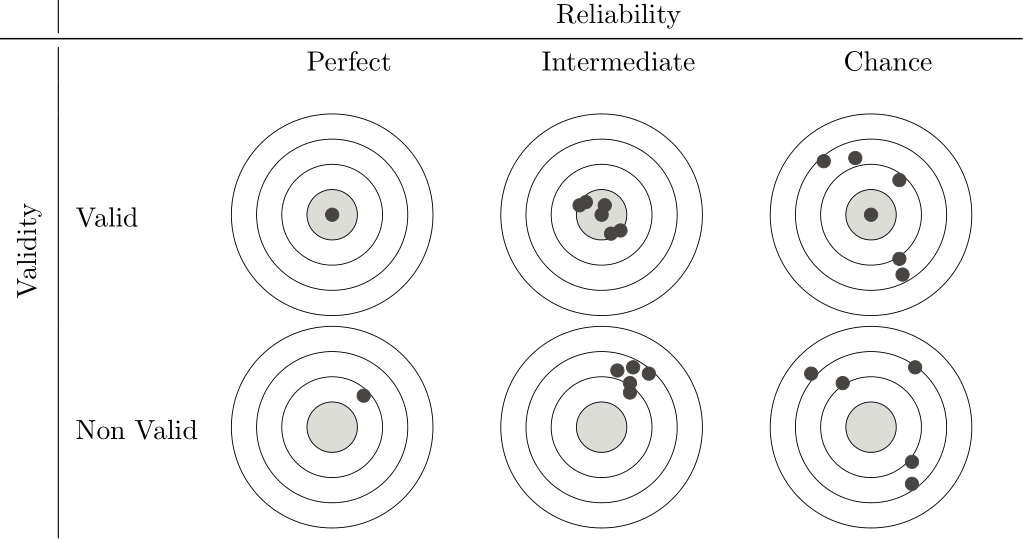
\includegraphics[width=1\linewidth]{figure/validity-reliability} \caption{Validity and Reliability}\label{fig:validity}
\end{figure}

Note that reliability and validity are not mutually exclusive. There is no point in having a highly valid measure that is not reliable, or a highly reliable measure that is not valid. Figure \ref{fig:validity}, after Krippendorff (\citeproc{ref-Krippendorff2019a}{2019}), shows this nicely by comparing our measure with a target, with the hits (the black dots) representing individual measures. What we are aiming for is at the top left: a measurement that hits the target perfectly every time. However, as our reliability decreases, more and more often we are not only hitting the target, but also hovering around it. As a result, high validity but low reliability means that sometimes we hit the target, but whether we do so is a matter of chance. At the same time, high reliability but low validity means that we hit the same spot every time, but always miss the target. So we never measure what we want to measure. So we want our measure to be both valid and reliable if it is to be of any use. Now, let's look at both concepts in a little more detail.

\subsection{Validity}\label{validity}

Of the two concepts, validity is the more difficult. To understand it a little better, we can divide it into three subtypes: content, criterion, and construct validity (\citeproc{ref-Carmines1979a}{Carmines \& Zeller, 1979}). Each of these focuses on a different aspect of validity and has different issues associated with it.

\begin{longtable}[]{@{}
  >{\raggedright\arraybackslash}p{(\linewidth - 2\tabcolsep) * \real{0.0538}}
  >{\raggedright\arraybackslash}p{(\linewidth - 2\tabcolsep) * \real{0.9462}}@{}}
\toprule\noalign{}
\endhead
\bottomrule\noalign{}
\endlastfoot
\textbf{Content Validity} & \emph{Does our measure cover all the aspects or dimensions of the concept we are studying?}

For example, if we design a coding scheme to measure `political ideology', have we included all the different attitudes to existing economic, social and foreign policy issues? To see if this is the case, we often rely on expert judgement and our own theoretical understanding of the concept. \\
\textbf{Criterion Validity} & \emph{How well does our measure correlate with other established measures of the same concept?}

For example, we might test whether a sentiment score we get from social media texts agrees with the results of a public opinion poll on the same topic. Another way might be to use our measure to predict a future outcome and then check that the prediction is correct. For example, we could see if the amount of attention given to specific policies in legislative debates could help us predict future budget allocations for those policies. \\
\textbf{Construct Validity} & \emph{How well does our measure operationalise our concept?}

If it does, we would expect the measure to behave in the same way as the concept. For example, if we develop a measure of ``economic uncertainty'' from news articles, we would expect it to be negatively correlated with measures of consumer confidence. \\
\end{longtable}

So, how do we put this into practice? One aspect that generally makes validity more difficult than reliability is that there is very little we can measure. Instead, we have to argue and prove, using a variety of methods, that our measure and overall analysis are indeed valid.

The most common approach is to compare against a \emph{gold standard}. For example, suppose we have access to a human-coded dataset for a subset of our data. In this case, we can compare the output of our (computational) method with these human judgments. Indeed, this is what we will do in Chapter \ref{supervised-methods}, where we will use this to calculate metrics such as accuracy, precision, recall and F1 scores. Related to this is when we use our data to predict other (external) data. For example, we might build a model to explain the overall economy of a country, and then relate this to the country's actual GDP. Somewhat more complicated is when we focus on our analysis's actual \emph{meaning}. This involves asking whether the results generated by our method are conceptually meaningful and make sense to people. In sentiment analysis, for example, we could manually review examples where our model gives strong positive or negative sentiment scores and see if they make sense. Preferably, we would have more than one person do this to avoid being too lenient on the model.

Ideally, we would use as many validation options as possible (a technique also known as triangulation). This way, with each validation, we build confidence and strengthen our argument that our approach is valid.

\subsection{Reliability}\label{reliability}

Reliability, as we saw above, is whether our measurement measures the same thing each time we do it, or, more broadly, whether our analysis would lead us to the same conclusions each time. One thing that helps us here is that reliability is something we can measure (unlike validity). It often comes in three forms: stability, reproducibility and accuracy. The first, \emph{Stability}, refers to how consistent a measurement is over time. For example, if we asked a coder to code the same text on different occasions, we would expect them to code it the same way (also known as within-coder consistency). The second, \emph{Reproducibility} (also known as inter-coder reliability), extends this to multiple coders. This means that independent coders, given the same coding instructions, should produce the same code for the same text. Finally, the third, \emph{Accuracy} (which we also use for validity), compares our coders' codes to a known standard or ``true'' value. The better the comparison, the more reliable our measure.

The first type - stability - is easy to measure: just repeat the analysis and compare the results. The second - reproducibility - is more complicated. This is because there are several things we want to be able to take into account, such as the ability to account for the categories our coders actually use, a standardised scale for interpretation, appropriateness to the level of measurement of our data (e.g.~nominal, ordinal, interval, ratio), correction for chance agreement, and the ability to handle missing data. There are several measures of reproducibility, each with its own strengths and limitations. The simplest and most straightforward is \emph{Percentage Agreement}, where we divide the number of codes the coders agree on by the total number of codes coded. However, this does not consider agreement that could occur purely by chance, therefore overestimates reliability.

Another way of doing this is to use Pearson's correlation coefficient (\emph{r}), as we would assume that we are correlating the codes of one or more coders. However, Pearson's \emph{r} measures linear association, not agreement. Thus, two coders can be in perfect disagreement and still show a strong positive or negative correlation if their disagreements follow a consistent linear pattern.

\begin{figure}
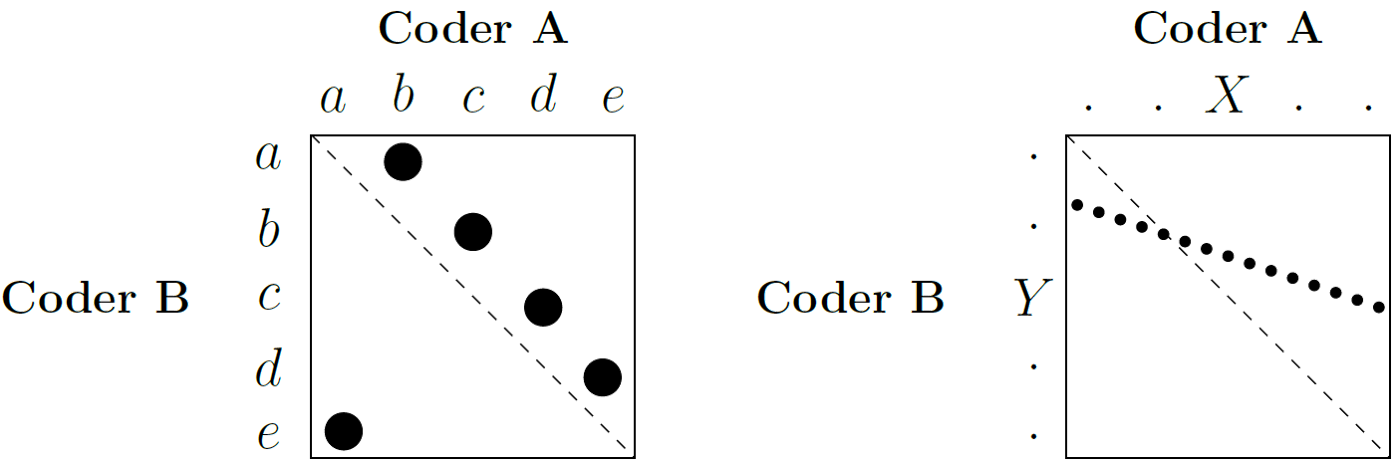
\includegraphics[width=1\linewidth]{figure/observers} \caption{Perfect agreement between two coders}\label{fig:coders}
\end{figure}

Consider Figure \ref{fig:coders}, which is an example adapted from Krippendorff (\citeproc{ref-Krippendorff2019a}{2019}) to illustrate this. Suppose we have two coders, A and B, each assigning sentences to five categories, labelled `a' to `e'. If, for example, whenever Coder A assigns `a', Coder B assigns `e'; and whenever Coder A assigns `b', Coder B assigns `a', and so on, they are in perfect disagreement (the example on the right). However, if we calculated Pearson's \emph{r}, we might still find a high correlation. This is because Pearson's \emph{r} only looks at the distances between the values, regardless of their location. For there to be a correlation, it is only necessary for increases or decreases in the category values assigned by one coder to be mirrored by similar directional changes in the other's assignments, a condition that can be met even when there is complete disagreement about the actual categories assigned. For this reason, we generally do not recommend it. Instead, we have the following options:

\textbf{Cohen's} \(\kappa\) is useful for assessing agreement between \emph{two coders} on \emph{nominal} (categorical) data. It improves on percent agreement because it corrects for chance agreement, based on each coder's individual marginal distributions of codes.

\textbf{Scott's} \(\pi\) is similar to Cohen's \(\kappa\), but we use it when we assume that the two coders are drawing from the same underlying distribution of codes. Consequently, it calculates the chance agreement based on the pooled marginal distribution of codes. Like Cohen's \(\kappa\), we use it with two coders and nominal data.

\textbf{Fleiss'} \(\kappa\) is an extension of Scott's \(\pi\) . We use it when assessing the agreement between \emph{multiple coders} (more than two) on \emph{nominal} data. A key requirement for Fleiss' \(\kappa\) is that each unit (e.g.~document, sentence) must be coded by the same number of coders, although it does not necessarily have to be the exact same set of coders for each unit.

Since each of these three measures has its drawbacks, we will use \textbf{Krippendorff's} \(\alpha\) here. It improves on the other measures by handling any number of coders, allowing for missing data, and applying to any level of measurement - nominal, ordinal, interval, and ratio. In addition, it calculates the random agreement based on the observed data, rather than assuming any distribution.

We can calculate Krippendorff's \(\alpha\) using the formula:

\[\alpha = 1 - \frac{D_o}{D_e}\]

Where \(D_o\) is the disagreement we observe between the coders, determined by the distance function we choose to be appropriate for the level of measurement of our data. \(D_e\) represents the disagreement we would expect by chance, calculated from the distribution of codes assigned by our coders. Thus, if we obtain a \(\alpha\) value of \(1.0\), this indicates perfect agreement; \(0.0\) indicates agreement at the level of chance alone; and a value below \(0.0\) indicates systematic disagreement between our coders. For interpretation, we follow Krippendorff's suggestion that a \(\alpha \ge 0.800\) indicates good reliability, while values between \(0.667 \le \alpha < 0.800\) may allow us to draw tentative conclusions. We usually consider alpha values below \(0.667\) to indicate poor reliability.

However, even \(\alpha\) has its limitations, the most problematic being when coders agree on only a few categories and use those categories very often. This inflates the value of \(\alpha\), making it higher than it should be.

\begin{figure}
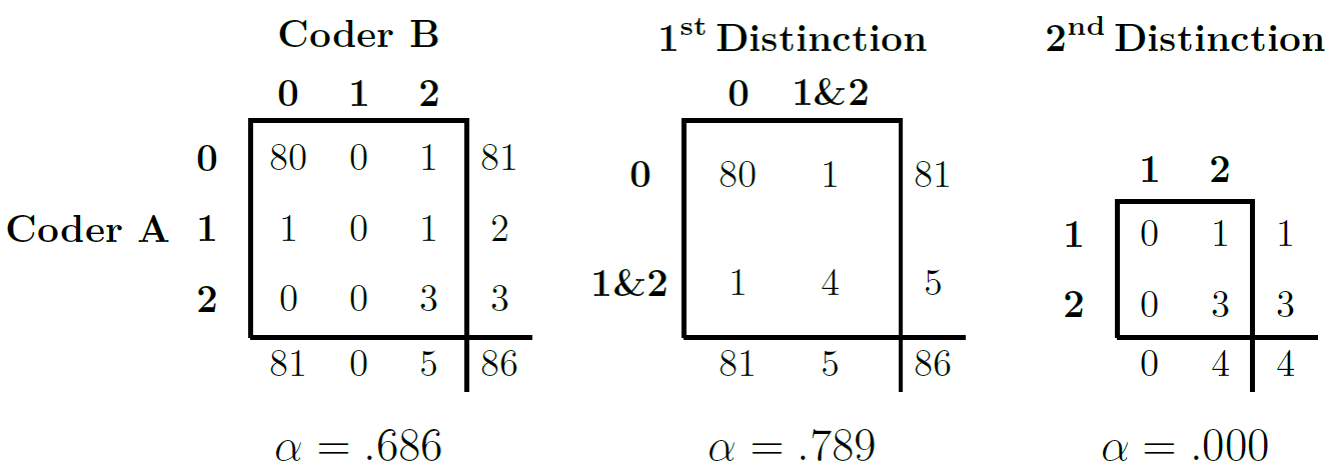
\includegraphics[width=1\linewidth]{figure/kripp} \caption{Inflation caused by use of a limited number of categories}\label{fig:kripp}
\end{figure}

Figure \ref{fig:kripp} (based on Krippendorff (\citeproc{ref-Krippendorff2019a}{2019})) illustrates this point. Imagine a coding task with three categories (\(0\), \(1\) and \(2\)). Category \(0\) indicates that the coders could not assign a more specific code, while categories \(1\) and \(2\) represent meaningful codes. If, out of a large number of cases (e.g.~\(86\)), both coders assign category \(0\) to the majority (e.g.~\(80\) cases), this leaves very few cases for us to observe agreement or disagreement on the meaningful categories \(1\) and \(2\). If we then calculate \(\alpha\) over all three categories, we get a moderate value (\(0.686\)). However, if we then collapse categories \(1\) and \(2\) into a single category `meaningful code', distinguishing only between `meaningful code' and `no meaningful code' (category \(0\)), the agreement on this broader distinction suddenly becomes very high, leading to a higher \(\alpha\) (\(0.789\)). On the other hand, if we remove the dominant \(0\) category and calculate \(\alpha\) only on categories \(1\) and \(2\) (for the few cases where they were used), the resulting \(\alpha\) could be very low (almost \(0\)). This could happen if a coder did not use one of these categories at all, even if they agreed on the other meaningful category in the remaining cases. This shows how our choice of categories to include in the calculation, and their observed distribution, can significantly influence the resulting \(\alpha\) value.

Finally, \(\alpha\) depends on our chosen metric (e.g.~nominal, ordinal, interval, ratio). If we use an inappropriate metric, such as a nominal metric for data that is actually ordinal, we may ignore valuable information about the ordered nature of the categories, leading us to misunderstand the actual level of agreement achieved by our coders.

To calculate \(\alpha\) in R, we use the \texttt{irr} package, which provides the \texttt{kripp.alpha()} function. To see how this works, we simulate a case where \(12\) coders code \(10\) sentences into \(3\) categories:

\begin{Shaded}
\begin{Highlighting}[]
\FunctionTok{library}\NormalTok{(irr)  }\CommentTok{\# Load the library}
\FunctionTok{set.seed}\NormalTok{(}\DecValTok{24}\NormalTok{)  }\CommentTok{\# Setting a seed makes our example reproducible}

\CommentTok{\# We create a matrix with 10 coders (rows) coding 12 sentences (columns) into 3}
\CommentTok{\# categories (1, 2, or 3)}

\NormalTok{reliability\_matrix }\OtherTok{\textless{}{-}} \FunctionTok{matrix}\NormalTok{(}\FunctionTok{sample}\NormalTok{(}\DecValTok{1}\SpecialCharTok{:}\DecValTok{3}\NormalTok{, }\DecValTok{10} \SpecialCharTok{*} \DecValTok{12}\NormalTok{, }\AttributeTok{replace =} \ConstantTok{TRUE}\NormalTok{), }\AttributeTok{nrow =} \DecValTok{10}\NormalTok{, }\AttributeTok{ncol =} \DecValTok{12}\NormalTok{)}

\CommentTok{\# Now, we calculate Krippendorff\textquotesingle{}s alpha, specifying the data and method (level}
\CommentTok{\# of measurement). For this example, we assume nominal data.}

\NormalTok{k\_alpha\_nominal }\OtherTok{\textless{}{-}} \FunctionTok{kripp.alpha}\NormalTok{(reliability\_matrix, }\AttributeTok{method =} \StringTok{"nominal"}\NormalTok{)}
\FunctionTok{print}\NormalTok{(k\_alpha\_nominal)}
\end{Highlighting}
\end{Shaded}

\begin{verbatim}
##  Krippendorff's alpha
## 
##  Subjects = 12 
##    Raters = 10 
##     alpha = 0.0106
\end{verbatim}

When we run \texttt{kripp.alpha}, the output typically includes the calculated \(\alpha\) value, the number of units (which it refers to as subjects), the number of coders (raters), and the level of measurement we specified for the calculation (e.g.~``nominal''). We then compare this resulting \(\alpha\) value with established thresholds (e.g.~\(0.67\) or \(0.80\), as Krippendorff suggests) to assess our coding reliability. For a more nuanced understanding of the stability of our estimate, we can obtain bootstrapped confidence intervals for \(\alpha\) using packages such as \texttt{kripp.boot} (see \href{https://github.com/MikeGruz/kripp.boot}{here}).

In addition, we can also visualise our reliability. One way of doing this, adapted from Benoit et al. (\citeproc{ref-Benoit2009a}{2009}) and Lowe \& Benoit (\citeproc{ref-Lowe2011a}{2011}), is to use bootstrapping to estimate and visualise the uncertainty around each coder's distribution of codes across the different categories. To do this, we first obtain the number of times each coder used each specific category. Then, for each coder, we use their observed coding patterns (i.e., the proportion of times they used each category) to repeatedly resample their codings, typically using a multinomial distribution. From these numerous bootstrapped samples, we compute summary statistics such as the mean percentage and standard error for each category for each coder. Finally, we plot these mean percentages along with their confidence intervals. This allows us to visually represent the consistency of each coder and identify any significant variation in their application of the coding scheme. As before, let's simulate the coding output of 12 coders across 3 categories and see how this works:

\begin{Shaded}
\begin{Highlighting}[]
\FunctionTok{library}\NormalTok{(dplyr)}
\FunctionTok{library}\NormalTok{(tidyr)}
\FunctionTok{library}\NormalTok{(ggplot2)}

\FunctionTok{set.seed}\NormalTok{(}\DecValTok{48}\NormalTok{)}

\CommentTok{\# Create placeholder data to simulate coder output. This tibble will have coder IDs and counts for three hypothetical categories (c00, c01, c02)}

\NormalTok{data\_uncertainty }\OtherTok{\textless{}{-}} \FunctionTok{tibble}\NormalTok{(}
  \AttributeTok{coderid =} \DecValTok{1}\SpecialCharTok{:}\DecValTok{12}\NormalTok{,}
  \AttributeTok{c00 =} \FunctionTok{rpois}\NormalTok{(}\DecValTok{12}\NormalTok{, }\DecValTok{50}\NormalTok{), }\CommentTok{\# Simulating counts for category 0}
  \AttributeTok{c01 =} \FunctionTok{rpois}\NormalTok{(}\DecValTok{12}\NormalTok{, }\DecValTok{20}\NormalTok{), }\CommentTok{\# Simulating counts for category 1}
  \AttributeTok{c02 =} \FunctionTok{rpois}\NormalTok{(}\DecValTok{12}\NormalTok{, }\DecValTok{10}\NormalTok{)  }\CommentTok{\# Simulating counts for category 2}
\NormalTok{) }\SpecialCharTok{\%\textgreater{}\%}
  \FunctionTok{mutate}\NormalTok{(}\AttributeTok{n =}\NormalTok{ c00 }\SpecialCharTok{+}\NormalTok{ c01 }\SpecialCharTok{+}\NormalTok{ c02) }\CommentTok{\# Total codes per coder}

\NormalTok{category\_cols\_id }\OtherTok{\textless{}{-}} \FunctionTok{c}\NormalTok{(}\StringTok{"c00"}\NormalTok{, }\StringTok{"c01"}\NormalTok{, }\StringTok{"c02"}\NormalTok{)}

\CommentTok{\# Now, we perform the bootstrap}
\NormalTok{n\_coders }\OtherTok{\textless{}{-}} \FunctionTok{nrow}\NormalTok{(data\_uncertainty)}
\NormalTok{n\_repl }\OtherTok{\textless{}{-}} \DecValTok{2000} \CommentTok{\# We set the number of bootstraps}
\NormalTok{n\_categories }\OtherTok{\textless{}{-}} \FunctionTok{length}\NormalTok{(category\_cols\_id)}

\CommentTok{\# We prepare an array to store our bootstrap results: coder x category x replicate}
\NormalTok{bootstrap\_results\_array }\OtherTok{\textless{}{-}} \FunctionTok{array}\NormalTok{(}
  \ConstantTok{NA}\NormalTok{,}
  \AttributeTok{dim =} \FunctionTok{c}\NormalTok{(n\_coders, n\_categories, n\_repl),}
  \AttributeTok{dimnames =} \FunctionTok{list}\NormalTok{(data\_uncertainty}\SpecialCharTok{$}\NormalTok{coderid, category\_cols\_id, }\DecValTok{1}\SpecialCharTok{:}\NormalTok{n\_repl)}
\NormalTok{)}

\CommentTok{\# We loop through each coder to resample their codings.}
\ControlFlowTok{for}\NormalTok{ (coder\_idx }\ControlFlowTok{in} \DecValTok{1}\SpecialCharTok{:}\NormalTok{n\_coders) \{}
\NormalTok{  observed\_counts }\OtherTok{\textless{}{-}} \FunctionTok{as.numeric}\NormalTok{(data\_uncertainty[coder\_idx, category\_cols\_id])}
\NormalTok{  total\_codes\_n }\OtherTok{\textless{}{-}}\NormalTok{ data\_uncertainty}\SpecialCharTok{$}\NormalTok{n[coder\_idx]}
  
\NormalTok{  observed\_probs }\OtherTok{\textless{}{-}}\NormalTok{ observed\_counts }\SpecialCharTok{/}\NormalTok{ total\_codes\_n}
  \CommentTok{\# We ensure probabilities sum to 1}
  \ControlFlowTok{if}\NormalTok{ (}\FunctionTok{abs}\NormalTok{(}\FunctionTok{sum}\NormalTok{(observed\_probs) }\SpecialCharTok{{-}} \DecValTok{1}\NormalTok{) }\SpecialCharTok{\textgreater{}} \FloatTok{1e{-}6}\NormalTok{) \{}
\NormalTok{    observed\_probs }\OtherTok{\textless{}{-}}\NormalTok{ observed\_probs }\SpecialCharTok{/} \FunctionTok{sum}\NormalTok{(observed\_probs)}
\NormalTok{  \}}
  
  \CommentTok{\# We perform multinomial resampling}
\NormalTok{  resampled\_counts\_matrix }\OtherTok{\textless{}{-}} \FunctionTok{rmultinom}\NormalTok{(}\AttributeTok{n =}\NormalTok{ n\_repl, }\AttributeTok{size =}\NormalTok{ total\_codes\_n, }\AttributeTok{prob =}\NormalTok{ observed\_probs)}
\NormalTok{  bootstrap\_results\_array[coder\_idx, , ] }\OtherTok{\textless{}{-}}\NormalTok{ resampled\_counts\_matrix}
  
\NormalTok{\}}

\CommentTok{\# We convert counts to percentages}
\NormalTok{bootstrap\_percentages\_array }\OtherTok{\textless{}{-}} \FunctionTok{sweep}\NormalTok{(}
\NormalTok{  bootstrap\_results\_array,}
  \AttributeTok{MARGIN =} \FunctionTok{c}\NormalTok{(}\DecValTok{1}\NormalTok{, }\DecValTok{3}\NormalTok{),}
\NormalTok{  data\_uncertainty}\SpecialCharTok{$}\NormalTok{n,}
  \AttributeTok{FUN =} \StringTok{"/"}
\NormalTok{) }\SpecialCharTok{*} \DecValTok{100}
\CommentTok{\# Handle potential NaN if a coder had 0 codes for \textquotesingle{}n\textquotesingle{}}
\NormalTok{bootstrap\_percentages\_array[}\FunctionTok{is.nan}\NormalTok{(bootstrap\_percentages\_array)] }\OtherTok{\textless{}{-}} \DecValTok{0}

\CommentTok{\# Calculate summary statistics}
\NormalTok{mean\_perc }\OtherTok{\textless{}{-}} \FunctionTok{apply}\NormalTok{(bootstrap\_percentages\_array, }\FunctionTok{c}\NormalTok{(}\DecValTok{1}\NormalTok{, }\DecValTok{2}\NormalTok{), mean, }\AttributeTok{na.rm =} \ConstantTok{TRUE}\NormalTok{)}
\CommentTok{\# Use the SD of the bootstrapped means as an estimate of the standard error}
\NormalTok{sd\_perc }\OtherTok{\textless{}{-}} \FunctionTok{apply}\NormalTok{(bootstrap\_percentages\_array, }\FunctionTok{c}\NormalTok{(}\DecValTok{1}\NormalTok{, }\DecValTok{2}\NormalTok{), sd, }\AttributeTok{na.rm =} \ConstantTok{TRUE}\NormalTok{)}

\NormalTok{mean\_perc\_df }\OtherTok{\textless{}{-}} \FunctionTok{as.data.frame.table}\NormalTok{(mean\_perc, }\AttributeTok{responseName =} \StringTok{"mean\_p"}\NormalTok{) }\SpecialCharTok{\%\textgreater{}\%}
  \FunctionTok{rename}\NormalTok{(}\AttributeTok{coderid =}\NormalTok{ Var1, }\AttributeTok{category =}\NormalTok{ Var2)}
\NormalTok{sd\_perc\_df }\OtherTok{\textless{}{-}} \FunctionTok{as.data.frame.table}\NormalTok{(sd\_perc, }\AttributeTok{responseName =} \StringTok{"se\_p"}\NormalTok{) }\SpecialCharTok{\%\textgreater{}\%}
  \FunctionTok{rename}\NormalTok{(}\AttributeTok{coderid =}\NormalTok{ Var1, }\AttributeTok{category =}\NormalTok{ Var2)}

\NormalTok{vis\_data }\OtherTok{\textless{}{-}} \FunctionTok{full\_join}\NormalTok{(mean\_perc\_df, sd\_perc\_df, }\AttributeTok{by =} \FunctionTok{c}\NormalTok{(}\StringTok{"coderid"}\NormalTok{, }\StringTok{"category"}\NormalTok{)) }\SpecialCharTok{\%\textgreater{}\%}
  \FunctionTok{mutate}\NormalTok{(}
    \AttributeTok{lower\_ci =}\NormalTok{ mean\_p }\SpecialCharTok{{-}} \FloatTok{1.96} \SpecialCharTok{*}\NormalTok{ se\_p, }\CommentTok{\# 95\% CI lower bound}
    \AttributeTok{upper\_ci =}\NormalTok{ mean\_p }\SpecialCharTok{+} \FloatTok{1.96} \SpecialCharTok{*}\NormalTok{ se\_p, }\CommentTok{\# 95\% CI upper bound}
    \AttributeTok{lower\_ci =} \FunctionTok{pmax}\NormalTok{(}\DecValTok{0}\NormalTok{, lower\_ci), }\CommentTok{\# Ensure CI doesn\textquotesingle{}t go below 0\%}
    \AttributeTok{upper\_ci =} \FunctionTok{pmin}\NormalTok{(}\DecValTok{100}\NormalTok{, upper\_ci), }\CommentTok{\# Ensure CI doesn\textquotesingle{}t exceed 100\%}
    \AttributeTok{coderid =} \FunctionTok{factor}\NormalTok{(coderid)        }\CommentTok{\# Treat coderid as a factor for plotting}
\NormalTok{  )}

\CommentTok{\# Finally, we plot the three categories:}

\NormalTok{categories\_to\_plot }\OtherTok{\textless{}{-}}\NormalTok{ category\_cols\_id[}\DecValTok{1}\SpecialCharTok{:}\FunctionTok{min}\NormalTok{(}\DecValTok{3}\NormalTok{, }\FunctionTok{length}\NormalTok{(category\_cols\_id))]}
\NormalTok{plots\_list }\OtherTok{\textless{}{-}} \FunctionTok{list}\NormalTok{() }\CommentTok{\# To store plots if we generate multiple}

\ControlFlowTok{for}\NormalTok{ (cat\_to\_plot }\ControlFlowTok{in}\NormalTok{ categories\_to\_plot) \{}
\NormalTok{  plot\_data\_subset }\OtherTok{\textless{}{-}} \FunctionTok{filter}\NormalTok{(vis\_data, category }\SpecialCharTok{==}\NormalTok{ cat\_to\_plot)}
  
\NormalTok{  p }\OtherTok{\textless{}{-}} \FunctionTok{ggplot}\NormalTok{(plot\_data\_subset, }\FunctionTok{aes}\NormalTok{(}\AttributeTok{x =}\NormalTok{ mean\_p, }\AttributeTok{y =}\NormalTok{ coderid)) }\SpecialCharTok{+}
    \FunctionTok{geom\_point}\NormalTok{(}\AttributeTok{size =} \DecValTok{2}\NormalTok{) }\SpecialCharTok{+}
    \FunctionTok{geom\_errorbarh}\NormalTok{(}\FunctionTok{aes}\NormalTok{(}\AttributeTok{xmin =}\NormalTok{ lower\_ci, }\AttributeTok{xmax =}\NormalTok{ upper\_ci),}
                   \AttributeTok{height =} \FloatTok{0.2}\NormalTok{,}
                   \AttributeTok{na.rm =} \ConstantTok{TRUE}\NormalTok{) }\SpecialCharTok{+}
    \FunctionTok{scale\_x\_continuous}\NormalTok{(}\AttributeTok{name =} \StringTok{"Mean Percentage Coded (\%) with 95\% CI"}\NormalTok{, }\AttributeTok{limits =} \FunctionTok{c}\NormalTok{(}\DecValTok{0}\NormalTok{, }\ConstantTok{NA}\NormalTok{)) }\SpecialCharTok{+}
    \FunctionTok{scale\_y\_discrete}\NormalTok{(}\AttributeTok{name =} \StringTok{"Coder ID"}\NormalTok{) }\SpecialCharTok{+}
    \FunctionTok{ggtitle}\NormalTok{(}\FunctionTok{paste}\NormalTok{(}\StringTok{"Our Analysis of Coder Usage for Category:"}\NormalTok{, cat\_to\_plot)) }\SpecialCharTok{+}
    \FunctionTok{theme\_classic}\NormalTok{()}
  
\NormalTok{  plots\_list[[cat\_to\_plot]] }\OtherTok{\textless{}{-}}\NormalTok{ p}
  \FunctionTok{print}\NormalTok{(p) }\CommentTok{\# Display the plot}
\NormalTok{\}}
\end{Highlighting}
\end{Shaded}

\pandocbounded{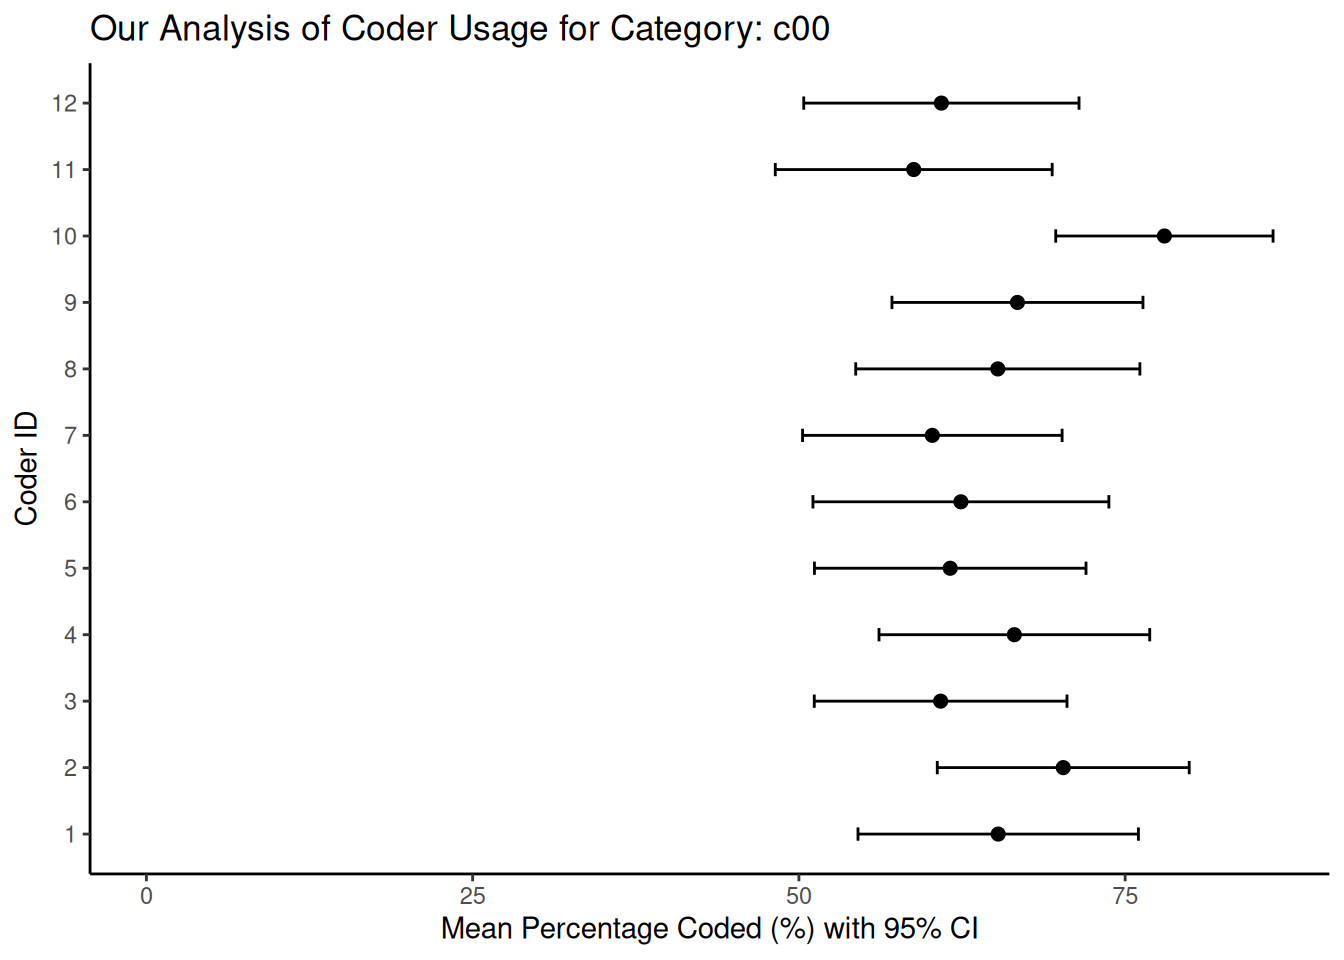
\includegraphics[keepaspectratio]{Introduction-to-Quantitative-Text-Analysis_files/figure-latex/reliability-bootstrap-1.pdf}} \pandocbounded{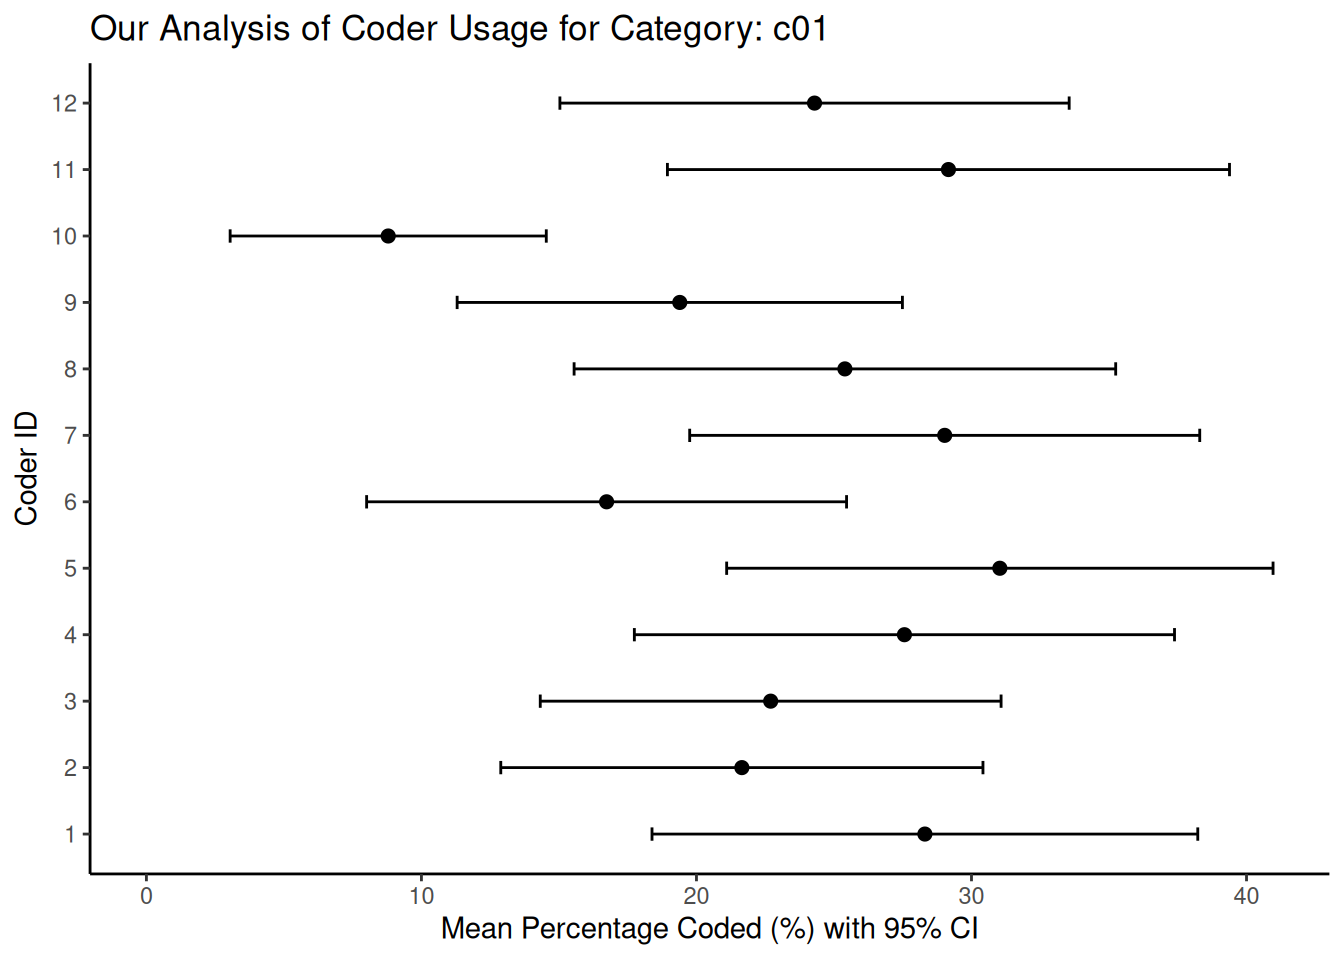
\includegraphics[keepaspectratio]{Introduction-to-Quantitative-Text-Analysis_files/figure-latex/reliability-bootstrap-2.pdf}} \pandocbounded{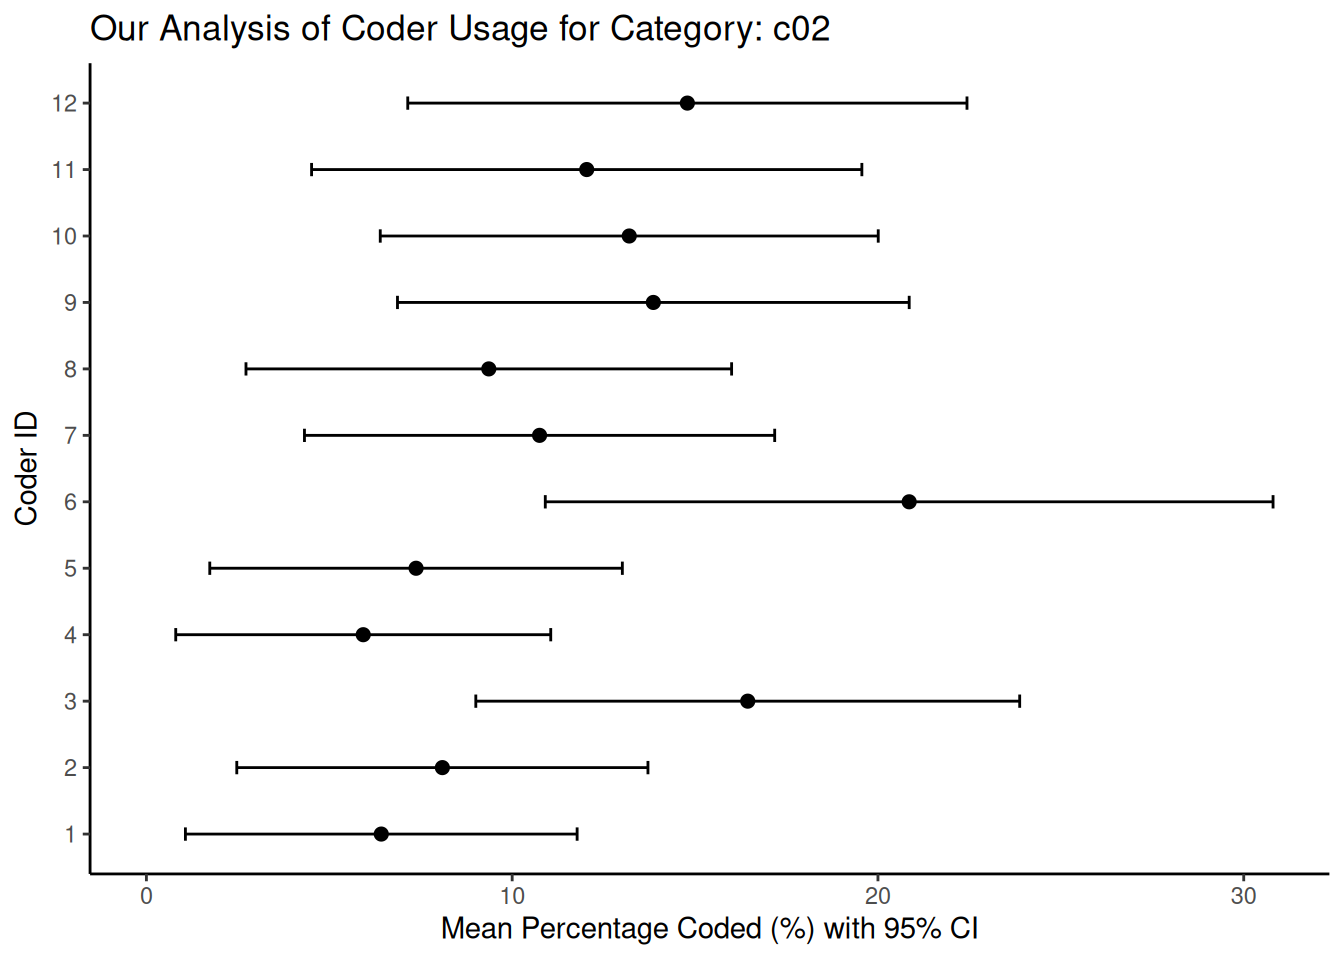
\includegraphics[keepaspectratio]{Introduction-to-Quantitative-Text-Analysis_files/figure-latex/reliability-bootstrap-3.pdf}}

In these plots, the horizontal bars represent the 95\% confidence intervals we derived from the bootstrap resampling process. When we see shorter bars around a coder's mean percentage, this indicates high consistency (low uncertainty) in that coder's use of that category relative to their overall coding activity. On the other hand, longer bars indicate greater uncertainty, which could be due to the coder's less frequent or less consistent use of that particular category. When comparing between coders, overlapping confidence intervals indicate that the coders used the category at statistically similar rates. However, non-overlapping intervals may indicate systematic differences in how a particular coder interpreted or applied a category compared to their peers. Graphs such as these can help us identify specific categories or coders that contribute most to disagreement, and we can use them to improve our coder training or refine our coding scheme.

\chapter{Text in R}\label{import}

No analysis is possible unless we have some data to work with. In this chapter, we will look at seven different ways of getting textual data into R: a) using .txt files, b) using .pdf files, c) using .csv files, d) using an API, e) using web scraping, f) using structured files such as JSON and XML, and g) importing from a database. However, before we look at these methods, let us first look at how R understands text and how we can work with it.

\section{Basics}\label{basics}

R treats text as a \emph{string} or \emph{character vector}, making it one of R's basic data structures, the others being logical, integer, real (numeric), complex, and raw. A character vector can contain a single string (such as a single word or phrase), while more complex character vectors can contain multiple strings, which could represent a collection of sentences, paragraphs, or even entire documents. Because character vectors are vectors, we can perform many of the same operations on them as we can on other vector types, such as calculations or checking their properties. For example, the \texttt{nchar()} function returns the number of characters \emph{within} each string element, while \texttt{length()} returns the number of \emph{elements} (or individual strings) contained in the vector.

Let's start by defining a character vector containing a single string and examining its properties using these two functions. Note that in R, we must enclose our strings in either double quotes (\texttt{"}) or single quotes (``\,`):

\begin{Shaded}
\begin{Highlighting}[]
\NormalTok{vector1 }\OtherTok{\textless{}{-}} \StringTok{"This is the first of our character vectors"}
\FunctionTok{nchar}\NormalTok{(vector1)  }\CommentTok{\# Number of characters in the string}
\FunctionTok{length}\NormalTok{(vector1)  }\CommentTok{\# Number of elements (strings) in the vector}
\end{Highlighting}
\end{Shaded}

As you can see from the output of the above code, the \texttt{nchar()} function tells us that the string has \(42\) characters. However, \texttt{length()} tells us the vector contains only \(1\) element. This is because \texttt{vector1} contains only a single string, even though that string is quite long. To illustrate a vector with multiple strings, we use the \texttt{c()} function (short for ``combine''). When used with strings, \texttt{c()} combines multiple individual strings into a single character vector. Let's create a vector with three different strings and see how \texttt{length()} and \texttt{nchar()} behave:

\begin{Shaded}
\begin{Highlighting}[]
\NormalTok{vector2 }\OtherTok{\textless{}{-}} \FunctionTok{c}\NormalTok{(}\StringTok{"This is one example"}\NormalTok{, }\StringTok{"This is another"}\NormalTok{, }\StringTok{"And so we can continue."}\NormalTok{)}
\FunctionTok{length}\NormalTok{(vector2)  }\CommentTok{\# Number of elements in vector}
\FunctionTok{nchar}\NormalTok{(vector2)  }\CommentTok{\# Returns characters for each element}
\FunctionTok{sum}\NormalTok{(}\FunctionTok{nchar}\NormalTok{(vector2))  }\CommentTok{\# Total number of characters in all elements}
\end{Highlighting}
\end{Shaded}

When we run this code, \texttt{length(vector2)} will return \(3\) because the vector contains three separate strings. As a result, \texttt{nchar(vector2)} now has multiple elements (3), and \texttt{nchar()} returns a vector of results, one for each string. To get the total number of characters in all three strings, we can wrap (or nest) \texttt{nchar(vector2)} inside the \texttt{sum()} function. Note that R typically evaluates commands from the inside out. So, it will first calculate the number of characters for each string in \texttt{vector2} (producing an intermediate numeric vector), after which the \texttt{sum()} function will calculate the sum of this intermediate vector.

The next step is to modify our vectors. For example, we can extract specific parts of a string and create substrings using the \texttt{substr(text,\ start\_position,\ end\_position)} function. To do so, we specify the starting and ending character positions. Note that the positions are counted from the beginning of the string, starting at 1 (and thus not 0):

\begin{Shaded}
\begin{Highlighting}[]
\FunctionTok{substr}\NormalTok{(vector1, }\DecValTok{1}\NormalTok{, }\DecValTok{5}\NormalTok{)  }\CommentTok{\# Extracts characters from position 1 to 5}
\FunctionTok{substr}\NormalTok{(vector1, }\DecValTok{7}\NormalTok{, }\DecValTok{11}\NormalTok{)  }\CommentTok{\# Extracts characters from position 7 to 11}
\end{Highlighting}
\end{Shaded}

Another thing we can do is combine multiple strings into a single one. The first way to do this is to use the \texttt{paste()} function and concatenate multiple strings into a single one. By default, \texttt{paste()} concatenates strings with a space in between, but we can change this using the \texttt{sep} argument. Another approach is to use a vector of multiple strings. In this case, we still use \texttt{paste()}, but now with the \texttt{collapse} argument:

\begin{Shaded}
\begin{Highlighting}[]
\NormalTok{fruits }\OtherTok{\textless{}{-}} \FunctionTok{paste}\NormalTok{(}\StringTok{"oranges"}\NormalTok{, }\StringTok{"lemons"}\NormalTok{, }\StringTok{"pears"}\NormalTok{, }\AttributeTok{sep =} \StringTok{"{-}"}\NormalTok{)}
\NormalTok{fruits}

\FunctionTok{paste}\NormalTok{(vector2, }\AttributeTok{collapse =} \StringTok{""}\NormalTok{)}
\end{Highlighting}
\end{Shaded}

We can also change the text itself, for example, changing its case (lowercase or uppercase) using \texttt{tolower()} (which converts all characters to lowercase) and \texttt{toupper()} (which converts them to uppercase):

\begin{Shaded}
\begin{Highlighting}[]
\NormalTok{sentences2 }\OtherTok{\textless{}{-}} \FunctionTok{c}\NormalTok{(}\StringTok{"This is a piece of example text"}\NormalTok{, }\StringTok{"This is another piece of example text"}\NormalTok{)}
\FunctionTok{tolower}\NormalTok{(sentences2)}
\FunctionTok{toupper}\NormalTok{(sentences2)}
\end{Highlighting}
\end{Shaded}

Another (and powerful) feature of R is its ability to find specific patterns within strings. These functions are especially powerful when combined with regular expressions (see for more on that \href{https://en.wikipedia.org/wiki/Regular_expression}{here}):

\begin{itemize}
\tightlist
\item
  \texttt{grep(pattern,\ x)}: This function searches for the specified \texttt{pattern} within each string element of the character vector \texttt{x}. It returns a vector of the \emph{indices} (positions) of the elements in \texttt{x} that contain a match for the pattern.
\item
  \texttt{grepl(pattern,\ x)}: Similar to \texttt{grep}, but instead of returning indices, it returns a \emph{logical vector} of the same length as \texttt{x}. Each element in the resulting vector is \texttt{TRUE} if the corresponding string in \texttt{x} matches the pattern and \texttt{FALSE} otherwise. This is useful for filtering or sub setting.
\item
  \texttt{sub(pattern,\ replacement,\ x)}: This function finds the specified \texttt{pattern} in each string element of \texttt{x} and replaces it with the \texttt{replacement} string. Importantly, \texttt{sub()} only replaces the \emph{first} occurrence of the pattern found within each string.
\item
  \texttt{gsub(pattern,\ replacement,\ x)}: This function is identical to \texttt{sub()}, but with one key difference: it replaces \emph{all} occurrences of the pattern found within each string element, not just the first one.
\end{itemize}

Let's see these pattern-matching and replacement functions in action:

\begin{Shaded}
\begin{Highlighting}[]
\NormalTok{text\_vector }\OtherTok{\textless{}{-}} \FunctionTok{c}\NormalTok{(}\StringTok{"This is a test sentence."}\NormalTok{, }\StringTok{"Another test here."}\NormalTok{, }\StringTok{"No match in this one."}\NormalTok{)}

\FunctionTok{grep}\NormalTok{(}\StringTok{"test"}\NormalTok{, text\_vector)  }\CommentTok{\# Find elements containing the exact word \textquotesingle{}test\textquotesingle{}}
\FunctionTok{grepl}\NormalTok{(}\StringTok{"test"}\NormalTok{, text\_vector)  }\CommentTok{\# Check which elements contain the word \textquotesingle{}test\textquotesingle{}}
\FunctionTok{sub}\NormalTok{(}\StringTok{"test"}\NormalTok{, }\StringTok{"sample"}\NormalTok{, text\_vector)  }\CommentTok{\# Replace the first instance of \textquotesingle{}test\textquotesingle{} with \textquotesingle{}sample\textquotesingle{} in each string}
\FunctionTok{gsub}\NormalTok{(}\StringTok{" "}\NormalTok{, }\StringTok{"\_"}\NormalTok{, text\_vector)  }\CommentTok{\# Replace all spaces \textquotesingle{} \textquotesingle{} with underscores \textquotesingle{}\_\textquotesingle{}}
\end{Highlighting}
\end{Shaded}

The opposite of pasting strings together is splitting them apart. The \texttt{strsplit(x,\ split)} function is designed to break down the elements of a character vector \texttt{x} into smaller pieces based on a specified \texttt{split} pattern (often a single character like a space, comma, or dash). Because each string in the input vector \texttt{x} might be split into a different number of resulting pieces, \texttt{strsplit()} returns a \emph{list}. Each element of this list corresponds to an original string from \texttt{x}, and within each list element is a character vector containing the substrings that resulted from the split.

\begin{Shaded}
\begin{Highlighting}[]
\NormalTok{sentence }\OtherTok{\textless{}{-}} \StringTok{"This sentence will be split into words"}
\FunctionTok{strsplit}\NormalTok{(sentence, }\StringTok{" "}\NormalTok{)  }\CommentTok{\# Splits the single string by spaces, returns a list with one element (a vector of words)}

\NormalTok{dates }\OtherTok{\textless{}{-}} \FunctionTok{c}\NormalTok{(}\StringTok{"2023{-}01{-}15"}\NormalTok{, }\StringTok{"2024{-}11{-}01"}\NormalTok{)}
\FunctionTok{strsplit}\NormalTok{(dates, }\StringTok{"{-}"}\NormalTok{)  }\CommentTok{\# Splits each date string by the dash, returns a list with two elements (vectors of year, month, day)}
\end{Highlighting}
\end{Shaded}

While basic functions like \texttt{print()} and \texttt{cat()} are sufficient for simple output, \texttt{sprintf()} provides much finer control over how numbers, strings, and other data types are formatted within a string, similar to the \texttt{printf} function found in C. You construct a format string containing placeholders (like \texttt{\%\ d\textquotesingle{}\ for\ integers,}\%s\texttt{for\ strings,}\%.2f\texttt{for\ floating-point\ numbers\ with\ two\ decimal\ places),\ and}sprintf()` replaces these placeholders with the values of subsequent arguments, respecting the specified formatting rules. This is particularly useful for creating consistent output or messages.

\begin{Shaded}
\begin{Highlighting}[]
\NormalTok{my\_var }\OtherTok{\textless{}{-}} \StringTok{"Hello"}
\FunctionTok{print}\NormalTok{(my\_var)  }\CommentTok{\# Prints the variable\textquotesingle{}s value, often with quotes for strings}
\FunctionTok{cat}\NormalTok{(my\_var, }\StringTok{"world!}\SpecialCharTok{\textbackslash{}n}\StringTok{"}\NormalTok{)  }\CommentTok{\# Concatenates and prints, useful for console output}

\NormalTok{value }\OtherTok{\textless{}{-}} \FloatTok{42.567}
\FunctionTok{sprintf}\NormalTok{(}\StringTok{"The value is \%.2f"}\NormalTok{, value)  }\CommentTok{\# Formats\textquotesingle{} value\textquotesingle{} to 2 decimal places within the string}
\FunctionTok{sprintf}\NormalTok{(}\StringTok{"Integer: \%d, String: \%s"}\NormalTok{, }\DecValTok{100}\NormalTok{, }\StringTok{"example"}\NormalTok{)  }\CommentTok{\# Inserts an integer and a string into the format string}
\end{Highlighting}
\end{Shaded}

While base R provides these essential tools for working with text, specialised packages such as \texttt{quanteda}, \texttt{tm}, \texttt{stringr}, or \texttt{tidytext} offer more comprehensive, efficient, and often more user-friendly functions for complex text processing and analysis tasks. These packages typically build upon the fundamental vector concepts and functions available in base R, providing extended capabilities that include more powerful regular expression handling, tokenisation, stemming, stop-word removal, and advanced text manipulation tools.

\section{Import .txt}\label{import-.txt}

Plain text (.txt) files are a standard, simple format for storing text due to their lack of formatting, small size, and cross-platform compatibility. The \texttt{readtext} package provides a convenient way to read text files. It automatically creates a data frame with text content and associated metadata, such as filenames. First, ensure the \texttt{readtext} package is installed (\texttt{install.packages("readtext")}) and loaded. Then, specify the directory containing your .txt files. It is good practice to use relative paths or R projects to manage file locations.

\begin{Shaded}
\begin{Highlighting}[]
\FunctionTok{library}\NormalTok{(readtext)}

\NormalTok{txt\_directory }\OtherTok{\textless{}{-}} \StringTok{"folder/txt"}  \CommentTok{\# Address of folder with the TXT files}

\CommentTok{\# The pattern \textquotesingle{}*\textquotesingle{} reads all files Encoding specifies the encoding the TXT}
\CommentTok{\# documents are in}

\NormalTok{data\_texts }\OtherTok{\textless{}{-}} \FunctionTok{readtext}\NormalTok{(}\FunctionTok{paste0}\NormalTok{(txt\_directory, }\StringTok{"/*.txt"}\NormalTok{), }\AttributeTok{docvarsfrom =} \StringTok{"filenames"}\NormalTok{,}
    \AttributeTok{encoding =} \StringTok{"UTF{-}8"}\NormalTok{)}
\end{Highlighting}
\end{Shaded}

In the last line, we set \texttt{docvarsfrom\ =\ "filenames"}. This creates a variable that stores the filenames alongside the text, allowing us to identify them later easily. In addition to \texttt{readtext}, base R functions like \texttt{readLines()} or \texttt{scan()} can also read .txt files, often line by line or into a single character vector, which may require further processing to organise by document.

\section{Import .pdf}\label{import-.pdf}

Importing PDF files is a bit more challenging than importing TXT files, as they often contain not only text but also complex formatting, images, and tables. To import them into R, we again use the \texttt{readtext} package (though, in this case, it will use \texttt{pdftools} in the background). Note that this only works with readable PDFs (where text can be selected/copied), not image-based scans. In case you have an image-based scan (basically a picture stored as a PDF), you first need to use Optical Character Recognition (OCR) to retrieve the text from it (there are various ways to do this, with \texttt{tesseract} being the most popular -- see for more on that \href{https://github.com/tesseract-ocr/tesseract}{here}).

\begin{Shaded}
\begin{Highlighting}[]
\FunctionTok{library}\NormalTok{(readtext)}

\NormalTok{pdf\_directory }\OtherTok{\textless{}{-}} \StringTok{"folder/pdf"}  \CommentTok{\# Address of folder with the PDF files}
\NormalTok{data\_pdf\_texts }\OtherTok{\textless{}{-}} \FunctionTok{readtext}\NormalTok{(}\FunctionTok{paste0}\NormalTok{(pdf\_files, }\StringTok{"/*.pdf"}\NormalTok{), }\AttributeTok{docvarsfrom =} \StringTok{"filenames"}\NormalTok{)}
\end{Highlighting}
\end{Shaded}

Also, remember that PDF text extraction is imperfect. Formatting, tables, headers/footers, and multi-column layouts can lead to jumbled text. Manual inspection and cleaning are often required.

\section{Import .csv}\label{import-.csv}

Sometimes, text data comes pre-processed as a document-term matrix (DTM) or term-frequency matrix stored in a CSV file. A DTM typically has documents as rows, terms (or words) as columns, and cell values representing the word counts. There are two main ways we can import CSV files: using R's inbuilt \texttt{read.csv()} or the \texttt{read\_csv} function from the \texttt{readr} package:

\begin{Shaded}
\begin{Highlighting}[]
\NormalTok{data\_dtm }\OtherTok{\textless{}{-}} \FunctionTok{read.csv}\NormalTok{(}\StringTok{"your\_dtm\_file.csv"}\NormalTok{)  }\CommentTok{\# In case the first row is NOT the column names}
\NormalTok{data\_dtm }\OtherTok{\textless{}{-}} \FunctionTok{read.csv}\NormalTok{(}\StringTok{"your\_dtm\_file.csv"}\NormalTok{, }\AttributeTok{header =} \ConstantTok{TRUE}\NormalTok{)}
\NormalTok{data\_dtm }\OtherTok{\textless{}{-}}\NormalTok{ readr}\SpecialCharTok{::}\FunctionTok{read\_csv}\NormalTok{(}\StringTok{"your\_dtm\_file.csv"}\NormalTok{, }\AttributeTok{col\_names =} \ConstantTok{FALSE}\NormalTok{)  }\CommentTok{\# In case the first row are NOT the column names}
\NormalTok{data\_dtm }\OtherTok{\textless{}{-}}\NormalTok{ readr}\SpecialCharTok{::}\FunctionTok{read\_csv}\NormalTok{(}\StringTok{"your\_dtm\_file.csv"}\NormalTok{)}
\end{Highlighting}
\end{Shaded}

Remember that importing a pre-computed matrix means you inherit the pre-processing choices made when it was created. Also, take into account that in some cases, the CSV is not delimited by a comma but by a semicolon (;) or tab. In that case, we have to import it as a delimited object:

\begin{Shaded}
\begin{Highlighting}[]
\NormalTok{data\_dtm }\OtherTok{\textless{}{-}} \FunctionTok{read\_delim}\NormalTok{(}\ConstantTok{NULL}\NormalTok{, }\AttributeTok{delim =} \StringTok{";"}\NormalTok{, }\AttributeTok{escape\_double =} \ConstantTok{FALSE}\NormalTok{)}
\NormalTok{data\_dtm }\OtherTok{\textless{}{-}} \FunctionTok{read\_delim}\NormalTok{(}\ConstantTok{NULL}\NormalTok{, }\AttributeTok{delim =} \StringTok{"}\SpecialCharTok{\textbackslash{}t}\StringTok{"}\NormalTok{, }\AttributeTok{escape\_double =} \ConstantTok{FALSE}\NormalTok{)}
\end{Highlighting}
\end{Shaded}

\section{Import from an API}\label{import-from-an-api}

Application Programming Interfaces (APIs) provide structured ways to request and receive data directly from web services (e.g., social media platforms, news organisations, databases). When available, using an API is generally more reliable and efficient than web scraping. There are some considerations to keep in mind:

\begin{itemize}
\tightlist
\item
  \textbf{Registration/Authentication}: Most APIs require registration to obtain an API key or token for authentication.
\item
  \textbf{Rate Limits}: APIs usually limit the requests allowed within a specific period.
\item
  \textbf{Terms of Service}: Always review the API's terms of service regarding data usage and restrictions.
\item
  \textbf{API Changes \& Restrictions}: APIs can change. Notably, access to platforms like Twitter/X and Facebook has become significantly restricted and often requires payment or enhanced verification. For instance, the \texttt{Rfacebook} package is no longer actively maintained. Always check the current status and documentation.
\item
  \textbf{R Packages}: Specific R packages often exist to simplify interaction with popular APIs (e.g., \texttt{rtweet} for Twitter/X, \texttt{RedditExtractoR} for Reddit, \texttt{WikipediR} for Wikipedia, \texttt{manifestoR} for the Manifesto Project corpus). If no dedicated package exists, you can use general HTTP packages like \texttt{httr} or \texttt{httr2} combined with \texttt{jsonlite} to handle requests and responses.
\end{itemize}

To demonstrate how this works, let us have a look at the New York Times Movie Reviews API (requires registering for an API key at \url{https://developer.nytimes.com/}):

\begin{Shaded}
\begin{Highlighting}[]
\FunctionTok{library}\NormalTok{(httr)}
\FunctionTok{library}\NormalTok{(jsonlite)}
\FunctionTok{library}\NormalTok{(tidyverse)}

\NormalTok{nyt\_api\_key }\OtherTok{\textless{}{-}} \StringTok{"[YOUR\_API\_KEY\_HERE]"}  \CommentTok{\# Replace \textquotesingle{}[YOUR\_API\_KEY\_HERE]\textquotesingle{} with your actual key}

\CommentTok{\# Construct the API request URL}
\NormalTok{base\_url }\OtherTok{\textless{}{-}} \StringTok{"[https://api.nytimes.com/svc/movies/v2/reviews/search.json](https://api.nytimes.com/svc/movies/v2/reviews/search.json)"}
\NormalTok{query\_params }\OtherTok{\textless{}{-}} \FunctionTok{list}\NormalTok{(}\AttributeTok{query =} \StringTok{"love"}\NormalTok{, }\StringTok{\textasciigrave{}}\AttributeTok{opening{-}date}\StringTok{\textasciigrave{}} \OtherTok{=} \StringTok{"2000{-}01{-}01:2020{-}01{-}01"}\NormalTok{, }\StringTok{\textasciigrave{}}\AttributeTok{api{-}key}\StringTok{\textasciigrave{}} \OtherTok{=}\NormalTok{ nyt\_api\_key)}

\NormalTok{response }\OtherTok{\textless{}{-}} \FunctionTok{GET}\NormalTok{(base\_url, }\AttributeTok{query =}\NormalTok{ query\_params)  }\CommentTok{\# Make the API request using httr::GET()}

\CommentTok{\# Parse the JSON content}
\NormalTok{content\_json }\OtherTok{\textless{}{-}} \FunctionTok{content}\NormalTok{(response, }\AttributeTok{as =} \StringTok{"text"}\NormalTok{, }\AttributeTok{encoding =} \StringTok{"UTF{-}8"}\NormalTok{)}
\NormalTok{reviews\_list }\OtherTok{\textless{}{-}} \FunctionTok{fromJSON}\NormalTok{(content\_json, }\AttributeTok{flatten =} \ConstantTok{TRUE}\NormalTok{)}
\NormalTok{reviews\_df }\OtherTok{\textless{}{-}} \FunctionTok{as\_tibble}\NormalTok{(reviews\_list}\SpecialCharTok{$}\NormalTok{results)  }\CommentTok{\# Convert the relevant part of the list (results) to a data frame}
\end{Highlighting}
\end{Shaded}

This example retrieves movie reviews published between 2000 and 2020 containing the word ``love''. The response is in JSON format, which \texttt{jsonlite::fromJSON()} converts into an R list, which is subsequently transformed into a \texttt{tibble} (a type of data frame).

\section{Import using Web Scraping}\label{import-using-web-scraping}

When an API is unavailable, web scraping---extracting data directly from the HTML structure of web pages---can be an alternative. Again, there are a few things to keep in mind:

\begin{itemize}
\tightlist
\item
  \textbf{Legality/Ethics}: Always check the website's \texttt{robots.txt} file (e.g., \texttt{www.example.com/robots.txt}) and Terms of Service before scraping. Many sites prohibit or restrict scraping. Respect website resources; avoid overly aggressive scraping that could overload servers.
\item
  \textbf{Website Structure}: Scraping relies on the stability of a website's HTML structure. If the site changes, your scraper might break.
\item
  \textbf{Static or Dynamic Content}: Simple websites with content loaded directly in the initial HTML are easier to scrape (using packages like \texttt{rvest}). Websites that load content dynamically using JavaScript after the initial page load often require browser automation tools, such as \texttt{RSelenium}.
\item
  \textbf{Complexity}: Scraping can be complex and requires knowledge of HTML and CSS selectors (or XPath).
\end{itemize}

To see how scraping works, let us scrape the page on the Cold War from Wikipedia using \texttt{rvest}:

\begin{Shaded}
\begin{Highlighting}[]
\CommentTok{\# Load necessary libraries}
\FunctionTok{library}\NormalTok{(rvest)}
\FunctionTok{library}\NormalTok{(dplyr)}
\FunctionTok{library}\NormalTok{(stringr)}
\FunctionTok{library}\NormalTok{(tibble)}

\CommentTok{\# Define the URL of the Wikipedia page}
\NormalTok{url }\OtherTok{\textless{}{-}} \StringTok{"https://en.wikipedia.org/wiki/Cold\_War"}

\CommentTok{\# Read the HTML content from the page}
\NormalTok{html\_content }\OtherTok{\textless{}{-}} \FunctionTok{read\_html}\NormalTok{(url)}
\end{Highlighting}
\end{Shaded}

Now, we need to identify the HTML elements containing the desired text. Using browser developer tools (often opened with F12 or Cmd+Shift+C) helps inspect the page structure. The main content paragraphs for Wikipedia articles are typically within \texttt{\textless{}p\textgreater{}}tags inside a main content \texttt{div}:

\begin{Shaded}
\begin{Highlighting}[]
\CommentTok{\# Extract paragraph text from the content section}
\NormalTok{paragraphs }\OtherTok{\textless{}{-}}\NormalTok{ html\_content }\SpecialCharTok{\%\textgreater{}\%}
    \FunctionTok{html\_nodes}\NormalTok{(}\StringTok{"\#mw{-}content{-}text .mw{-}parser{-}output p"}\NormalTok{) }\SpecialCharTok{\%\textgreater{}\%}
    \FunctionTok{html\_text2}\NormalTok{()  }\CommentTok{\# Extract text, attempting to preserve formatting like line breaks}

\NormalTok{coldwar\_text\_df }\OtherTok{\textless{}{-}} \FunctionTok{tibble}\NormalTok{(}\AttributeTok{paragraph =}\NormalTok{ paragraphs)  }\CommentTok{\# Convert to a tibble/data frame}
\NormalTok{coldwar\_text\_df }\OtherTok{\textless{}{-}}\NormalTok{ coldwar\_text\_df }\SpecialCharTok{\%\textgreater{}\%}
    \FunctionTok{filter}\NormalTok{(}\FunctionTok{nchar}\NormalTok{(}\FunctionTok{trimws}\NormalTok{(paragraph)) }\SpecialCharTok{\textgreater{}} \DecValTok{0}\NormalTok{)  }\CommentTok{\# Remove empty or whitespace{-}only paragraphs}

\CommentTok{\# Extract paragraph text from the content section}
\NormalTok{paragraphs }\OtherTok{\textless{}{-}}\NormalTok{ html\_content }\SpecialCharTok{\%\textgreater{}\%}
    \FunctionTok{html\_nodes}\NormalTok{(}\StringTok{"\#mw{-}content{-}text .mw{-}parser{-}output p"}\NormalTok{) }\SpecialCharTok{\%\textgreater{}\%}
    \FunctionTok{html\_text2}\NormalTok{()  }\CommentTok{\# Extracts text while preserving formatting}

\CommentTok{\# Convert to a tibble and remove empty/whitespace{-}only paragraphs}
\NormalTok{coldwar\_text\_df }\OtherTok{\textless{}{-}} \FunctionTok{tibble}\NormalTok{(}\AttributeTok{paragraph =}\NormalTok{ paragraphs) }\SpecialCharTok{\%\textgreater{}\%}
    \FunctionTok{filter}\NormalTok{(}\FunctionTok{nchar}\NormalTok{(}\FunctionTok{trimws}\NormalTok{(paragraph)) }\SpecialCharTok{\textgreater{}} \DecValTok{0}\NormalTok{)}

\CommentTok{\# Display the first few rows}
\FunctionTok{print}\NormalTok{(}\FunctionTok{head}\NormalTok{(coldwar\_text\_df))}
\end{Highlighting}
\end{Shaded}

For more complex scraping involving logins, button clicks, or dynamically loaded content, explore the \texttt{RSelenium} package, which programmatically controls a web browser. For more on web scraping, see Wickham et al. (\citeproc{ref-Wickham2023a}{2023}), with the book being available \href{https://r4ds.hadley.nz/webscraping.html}{here}.

\section{Import JSON and XML}\label{import-json-and-xml}

JSON (JavaScript Object Notation) and XML (eXtensible Markup Language) are standard hierarchical data formats often obtained from APIs or other data sources. For JSON, we use the \texttt{jsonlite} package. Here, \texttt{fromJSON()} reads JSON files or text into R lists or data frames. Note that the path does not need to refer to a place on your computer but can also be an address to an online API:

\begin{Shaded}
\begin{Highlighting}[]
\FunctionTok{library}\NormalTok{(jsonlite)}
\NormalTok{my\_data\_df }\OtherTok{\textless{}{-}} \FunctionTok{fromJSON}\NormalTok{(}\StringTok{"path/to/your/data.json"}\NormalTok{, }\AttributeTok{flatten =} \ConstantTok{TRUE}\NormalTok{)  }\CommentTok{\# Here, \textasciigrave{}\textasciigrave{}flatten = TRUE\textasciigrave{}\textasciigrave{} flattens the object into a data frame}
\end{Highlighting}
\end{Shaded}

For XML, we use the \texttt{xml2} package. It provides functions like \texttt{read\_xml()} or \texttt{read\_html()} to parse files/URLs, and \texttt{xml\_find\_all()} (with XPath expressions), \texttt{xml\_text()}, \texttt{xml\_attr()} etc., to navigate and extract data:

\begin{Shaded}
\begin{Highlighting}[]
\FunctionTok{library}\NormalTok{(xml2)}
\NormalTok{xml\_doc }\OtherTok{\textless{}{-}} \FunctionTok{read\_xml}\NormalTok{(}\StringTok{"path/to/your/data.xml"}\NormalTok{)}
\NormalTok{titles }\OtherTok{\textless{}{-}} \FunctionTok{xml\_find\_all}\NormalTok{(xml\_doc, }\StringTok{".//title"}\NormalTok{) }\SpecialCharTok{\%\textgreater{}\%}
    \FunctionTok{xml\_text}\NormalTok{()  }\CommentTok{\# Find specific nodes using XPath and extract text (here \textless{}title\textgreater{})}
\end{Highlighting}
\end{Shaded}

\section{Import from Databases}\label{import-from-databases}

If your text data is somewhere in a relational database (like PostgreSQL, MySQL, SQLite, etc.), you can connect directly from R using the \texttt{DBI} (Database Interface) package along with a specific backend package for your database type, such as \texttt{RPostgres}, \texttt{RMariaDB}, \texttt{RSQLite}, \texttt{odbc}. Here, let us try to import a PostgreSQL database file:

\begin{Shaded}
\begin{Highlighting}[]
\FunctionTok{library}\NormalTok{(DBI)}
\FunctionTok{library}\NormalTok{(RSQLite)  }\CommentTok{\# Load the specific backend}

\NormalTok{connection }\OtherTok{\textless{}{-}} \FunctionTok{dbConnect}\NormalTok{(RPostgres}\SpecialCharTok{::}\FunctionTok{Postgres}\NormalTok{(), }\AttributeTok{dbname =} \StringTok{"your\_db"}\NormalTok{, }\AttributeTok{host =} \StringTok{"your\_host"}\NormalTok{,}
    \AttributeTok{port =} \DecValTok{5432}\NormalTok{, }\AttributeTok{user =} \StringTok{"your\_user"}\NormalTok{, }\AttributeTok{password =} \StringTok{"your\_password"}\NormalTok{)}

\FunctionTok{print}\NormalTok{(}\FunctionTok{dbListTables}\NormalTok{(connection))  }\CommentTok{\# List available tables}

\NormalTok{query }\OtherTok{\textless{}{-}} \StringTok{"SELECT doc\_id, text\_content FROM documents WHERE year = 2023;"}  \CommentTok{\# Query the database using SQL}
\NormalTok{results\_df }\OtherTok{\textless{}{-}} \FunctionTok{dbGetQuery}\NormalTok{(connection, query)}

\FunctionTok{dbDisconnect}\NormalTok{(connection)}
\end{Highlighting}
\end{Shaded}

\chapter{Describe}\label{describe}

Now that we have loaded our texts into R, it is time to understand \emph{what} our texts are about, who their authors are, and what we expect to find in them. This chapter focuses on techniques for exploring and summarising text data, including keywords-in-context, visualisations, and text statistics. Before diving into these techniques, we will briefly discuss the concept of the \emph{corpus}, which is central to working with text data in \texttt{quanteda} and the \emph{DFM} (data-frequency matrix), which we derive from it. Throughout this chapter, we will use the example of the Manifesto Project corpus, specifically the UK manifestos, to illustrate these concepts and techniques. This data is part of the \texttt{quanteda.corpora} package as \texttt{data\_corpus\_ukmanifestos}.

\section{Corpus and DFM}\label{corpus-and-dfm}

In \texttt{quanteda}, the primary object for storing and managing text data is the \texttt{corpus}. A \texttt{corpus} object holds your documents and any associated metadata, known as \emph{document-level variables} or \emph{docvars}. The key characteristic of a \texttt{corpus} object is that it remains immutable during your analysis. Instead of modifying the original corpus, you create derivative objects (like tokens or document-feature matrices) for analysis. This approach ensures reproducibility and allows you to easily return to your original data for different analyses or pre-processing steps.

Creating a corpus in \texttt{quanteda} is straightforward. As seen in the \ref{import} chapter, one standard method is to use the \texttt{readtext} package, which reads various file formats and creates a data frame with document IDs and text. This data frame can be directly converted into a \texttt{corpus} object using the \texttt{corpus()} function.

Alternatively, you can create a corpus from a simple character vector, where each element represents a document. If the vector elements are named, these names will be used as document identifiers (\texttt{doc\_id}); otherwise, \texttt{quanteda} will generate default IDs.

Incorporating document-level variables (docvars) is highly recommended. These variables store crucial metadata about each document, such as the author, publication date, source, or other relevant categorical or numerical information. Docvars are essential for grouping, filtering, and conducting analyses that relate textual features to external characteristics of the documents. When you create a corpus from a data frame, \texttt{quanteda} automatically attempts to include other columns as docvars. You can add or modify docvars later using the \texttt{docvars()} function.

\begin{Shaded}
\begin{Highlighting}[]
\FunctionTok{library}\NormalTok{(quanteda)  }\CommentTok{\# Core text analysis functions}
\FunctionTok{library}\NormalTok{(quanteda.corpora)  }\CommentTok{\# Access to built{-}in text corpora}
\FunctionTok{library}\NormalTok{(quanteda.textstats)  }\CommentTok{\# Text statistics}
\FunctionTok{library}\NormalTok{(quanteda.textplots)  }\CommentTok{\# Visualizing text statistics}
\FunctionTok{library}\NormalTok{(ggplot2)  }\CommentTok{\# Plots}
\FunctionTok{library}\NormalTok{(reshape2)  }\CommentTok{\# For melting data frames }

\FunctionTok{data}\NormalTok{(data\_corpus\_ukmanifestos)  }\CommentTok{\# Load the UK political manifestos corpus}

\NormalTok{selected\_parties }\OtherTok{\textless{}{-}} \FunctionTok{c}\NormalTok{(}\StringTok{"Con"}\NormalTok{, }\StringTok{"Lab"}\NormalTok{, }\StringTok{"LD"}\NormalTok{, }\StringTok{"UKIP"}\NormalTok{, }\StringTok{"SNP"}\NormalTok{, }\StringTok{"PCy"}\NormalTok{, }\StringTok{"SF"}\NormalTok{)  }\CommentTok{\# Filter the corpus to include only documents from the year 1997 onwards and belonging to a selected set of political parties}
\NormalTok{data\_corpus\_ukmanifestos }\OtherTok{\textless{}{-}} \FunctionTok{corpus\_subset}\NormalTok{(data\_corpus\_ukmanifestos, Year }\SpecialCharTok{\textgreater{}} \DecValTok{1996} \SpecialCharTok{\&}
\NormalTok{    Party }\SpecialCharTok{\%in\%}\NormalTok{ selected\_parties)}
\end{Highlighting}
\end{Shaded}

The \emph{document-feature matrix} (DFM) is the core data structure for many quantitative text analysis methods. It represents the corpus as a matrix, where documents are represented as rows and features (typically words or n-grams, after pre-processing) are represented as columns. The cell values are usually the counts of each feature in each document. The DFM is created from a \texttt{tokens} object (which identifies the individual words in a document) using the \texttt{dfm()} function.

\begin{Shaded}
\begin{Highlighting}[]
\NormalTok{data\_tokens }\OtherTok{\textless{}{-}} \FunctionTok{tokens}\NormalTok{(data\_corpus\_ukmanifestos)}
\NormalTok{data\_dfm }\OtherTok{\textless{}{-}} \FunctionTok{dfm}\NormalTok{(data\_tokens)}

\FunctionTok{head}\NormalTok{(data\_dfm)}
\end{Highlighting}
\end{Shaded}

By default, \texttt{dfm()} counts the occurrences of each feature (term frequency). If you want to, you can apply different weighting schemes like TF-IDF using \texttt{dfm\_tfidf()} to emphasise words that are more important to a document relative to the corpus. However, at this point, the DFM contains much information we do not need, such as words like `the' and `1997'. Because of this, we rarely generate the DFM directly, but we first carry out some pre-processing, to which we will now turn.

\section{Text Pre-processing}\label{text-pre-processing}

Raw text data is inherently complex and often contains noise that can obscure patterns relevant to your research question. Text pre-processing is the cleaning and normalising of text to make it suitable for quantitative analysis. These steps transform the raw text into a structured format, such as a document-feature matrix, by reducing variability and focusing on meaningful units of text.

Choosing the proper pre-processing steps is not trivial and heavily depends on your research question and the nature of your text data. As highlighted by Denny \& Spirling (\citeproc{ref-Denny2018a}{2018}), different pre-processing choices can significantly impact the results of downstream analyses, particularly unsupervised methods like topic modelling or clustering. Understanding what each pre-processing step does and its potential consequences is crucial. The \texttt{preText} R package, developed by the authors of that paper, provides tools to evaluate the sensitivity of your results to different pre-processing pipelines.

Pre-processing is typically applied sequentially to the text. In \texttt{quanteda}, most pre-processing steps operate on a \texttt{tokens} object, transforming each document's list of word sequences before creating the final document-feature matrix.

\subsection{Tokenisation and Initial Cleaning}\label{tokenisation-and-initial-cleaning}

The first step in pre-processing is \emph{tokenisation}: splitting the continuous text into discrete units called tokens. These are usually individual words but can also be sentences, paragraphs, or characters. \texttt{quanteda}'s \texttt{tokens()} function is used for this and allows for initial cleaning during the tokenisation process. By default, \texttt{tokens()} splits on whitespace and keeps punctuation, symbols, and numbers:

\begin{Shaded}
\begin{Highlighting}[]
\NormalTok{data\_tokens }\OtherTok{\textless{}{-}} \FunctionTok{tokens}\NormalTok{(data\_corpus\_ukmanifestos)}
\FunctionTok{head}\NormalTok{(data\_tokens[[}\DecValTok{5}\NormalTok{]], }\DecValTok{20}\NormalTok{)}
\end{Highlighting}
\end{Shaded}

\begin{verbatim}
##  [1] "Manifesto"   "May"         "1997"        "Contents"    ":"          
##  [6] "*"           "A"           "New"         "Opportunity" "for"        
## [11] "Peace"       "*"           "Unionists"   "*"           "Economy"    
## [16] "*"           "Social"      "Justice"     "and"         "Economic"
\end{verbatim}

The \texttt{head(data\_tokens{[}{[}5{]}{]},\ 20)} argument here allows us to see the first \(20\) terms of the 5th object in our corpus (the 1997 Sinn Féin manifesto). As we can see, the raw tokens here include punctuation, numbers and symbols, as \texttt{tokens()} does not remove those unless we specify this:

\begin{Shaded}
\begin{Highlighting}[]
\NormalTok{data\_tokens\_cleaned }\OtherTok{\textless{}{-}} \FunctionTok{tokens}\NormalTok{(}
\NormalTok{  data\_corpus\_ukmanifestos,}
  \AttributeTok{what =} \StringTok{"word"}\NormalTok{,}
  \CommentTok{\# Specify that we want to tokenise into words}
  \AttributeTok{remove\_punct =} \ConstantTok{TRUE}\NormalTok{,}
  \CommentTok{\# Remove punctuation marks like ., !?}
  \AttributeTok{remove\_symbols =} \ConstantTok{TRUE}\NormalTok{,}
  \CommentTok{\# Remove symbols like $, \%, \^{}, \&, *}
  \AttributeTok{remove\_numbers =} \ConstantTok{TRUE}\NormalTok{,}
  \CommentTok{\# Remove numerical digits (e.g., 123, 1997)}
  \AttributeTok{remove\_url =} \ConstantTok{TRUE}\NormalTok{,}
  \CommentTok{\# Remove URLs (web addresses).}
  \AttributeTok{remove\_separators =} \ConstantTok{TRUE}\NormalTok{,}
  \CommentTok{\# Remove separator characters like tabs, newlines, and multiple spaces.}
  \AttributeTok{split\_hyphens =} \ConstantTok{FALSE}\NormalTok{,}
  \CommentTok{\# If false, words such as matter{-}of{-}fact will not be split}
  \AttributeTok{split\_tags =} \ConstantTok{FALSE}\NormalTok{,}
  \CommentTok{\# If false, do not split social media tags}
  \AttributeTok{include\_docvars =} \ConstantTok{TRUE}\NormalTok{,}
  \AttributeTok{concatenator =} \StringTok{"\_"}\NormalTok{,}
  \CommentTok{\# The character to connect tokens that should stay together (e.g. we can write conservative\_party to prevent it from being split)}
  \AttributeTok{verbose =} \FunctionTok{quanteda\_options}\NormalTok{(}\StringTok{"verbose"}\NormalTok{)}
\NormalTok{)}

\CommentTok{\# Display the first 20 tokens of the first document after initial cleaning to observe the removal of specified elements.}
\FunctionTok{head}\NormalTok{(data\_tokens\_cleaned[[}\DecValTok{5}\NormalTok{]], }\DecValTok{20}\NormalTok{)}
\end{Highlighting}
\end{Shaded}

\begin{verbatim}
##  [1] "Manifesto"   "May"         "Contents"    "A"           "New"        
##  [6] "Opportunity" "for"         "Peace"       "Unionists"   "Economy"    
## [11] "Social"      "Justice"     "and"         "Economic"    "Equality"   
## [16] "Young"       "People's"    "Rights"      "Education"   "And"
\end{verbatim}

\begin{Shaded}
\begin{Highlighting}[]
\FunctionTok{ntoken}\NormalTok{(data\_tokens\_cleaned) }\CommentTok{\# The number of tokens per document}
\end{Highlighting}
\end{Shaded}

\begin{verbatim}
##  UK_natl_1997_en_Con  UK_natl_1997_en_Lab   UK_natl_1997_en_LD 
##                20796                17456                14080 
##  UK_natl_1997_en_PCy   UK_natl_1997_en_SF UK_natl_1997_en_UKIP 
##                16075                 5857                11839 
##  UK_natl_2001_en_Con  UK_natl_2001_en_Lab   UK_natl_2001_en_LD 
##                13142                28606                21101 
##  UK_natl_2001_en_PCy   UK_natl_2001_en_SF  UK_natl_2001_en_SNP 
##                 6542                 7061                10383 
##  UK_natl_2005_en_Con  UK_natl_2005_en_Lab   UK_natl_2005_en_LD 
##                 7606                23651                16033 
##  UK_natl_2005_en_PCy   UK_natl_2005_en_SF  UK_natl_2005_en_SNP 
##                 7289                20335                 2585 
## UK_natl_2005_en_UKIP  UK_regl_2003_en_PCy 
##                 8978                24971
\end{verbatim}

\begin{Shaded}
\begin{Highlighting}[]
\FunctionTok{ntype}\NormalTok{(data\_tokens\_cleaned) }\CommentTok{\# The number of unique tokens per document}
\end{Highlighting}
\end{Shaded}

\begin{verbatim}
##  UK_natl_1997_en_Con  UK_natl_1997_en_Lab   UK_natl_1997_en_LD 
##                 3043                 2930                 2756 
##  UK_natl_1997_en_PCy   UK_natl_1997_en_SF UK_natl_1997_en_UKIP 
##                 3215                 1741                 2774 
##  UK_natl_2001_en_Con  UK_natl_2001_en_Lab   UK_natl_2001_en_LD 
##                 2746                 4027                 3852 
##  UK_natl_2001_en_PCy   UK_natl_2001_en_SF  UK_natl_2001_en_SNP 
##                 1639                 2010                 2366 
##  UK_natl_2005_en_Con  UK_natl_2005_en_Lab   UK_natl_2005_en_LD 
##                 2027                 3903                 3207 
##  UK_natl_2005_en_PCy   UK_natl_2005_en_SF  UK_natl_2005_en_SNP 
##                 1904                 4256                 1008 
## UK_natl_2005_en_UKIP  UK_regl_2003_en_PCy 
##                 2434                 3937
\end{verbatim}

The \texttt{remove\_*} arguments in \texttt{tokens()} are powerful for initial cleaning, simplifying the token set by removing elements that might not be relevant to your analysis and reducing noise. Also note that even though we remove punctuation, this is not always the case, such as when we are dealing with a possessive apostrophe (as in People's). We could (if we wanted to) remove this as well, by adding \texttt{tokens\_remove(pattern\ =\ "\textquotesingle{}s\$",\ valuetype\ =\ "regex")}, though we do not recommend this as this would leave the \texttt{s} as a single character.

\subsection{Lower-casing}\label{lower-casing}

Converting all text to lower-case is a standard normalisation step. It ensures that the same word is not counted as different features simply because of variations in capitalisation (e.g., ``Party'', ``party'', ``PARTY''). This step is crucial for consistent term counting, and we generally recommend it unless your analysis requires preserving case information (e.g., for Named Entity Recognition). \texttt{quanteda} provides the \texttt{tokens\_tolower()} function. Note that \texttt{keep\_acronyms=FALSE} ensures that acronyms (like NATO) are also lower-cased. Set to \texttt{TRUE} if you want to preserve the capitalisation of detected acronyms:

\begin{Shaded}
\begin{Highlighting}[]
\NormalTok{data\_tokens\_lower }\OtherTok{\textless{}{-}} \FunctionTok{tokens\_tolower}\NormalTok{(data\_tokens\_cleaned, }\AttributeTok{keep\_acronyms =} \ConstantTok{FALSE}\NormalTok{)}
\FunctionTok{head}\NormalTok{(data\_tokens\_lower[[}\DecValTok{5}\NormalTok{]], }\DecValTok{20}\NormalTok{)}
\end{Highlighting}
\end{Shaded}

\begin{verbatim}
##  [1] "manifesto"   "may"         "contents"    "a"           "new"        
##  [6] "opportunity" "for"         "peace"       "unionists"   "economy"    
## [11] "social"      "justice"     "and"         "economic"    "equality"   
## [16] "young"       "people's"    "rights"      "education"   "and"
\end{verbatim}

\begin{Shaded}
\begin{Highlighting}[]
\FunctionTok{ntoken}\NormalTok{(data\_tokens\_lower)  }\CommentTok{\# The number of tokens per document}
\end{Highlighting}
\end{Shaded}

\begin{verbatim}
##  UK_natl_1997_en_Con  UK_natl_1997_en_Lab   UK_natl_1997_en_LD 
##                20796                17456                14080 
##  UK_natl_1997_en_PCy   UK_natl_1997_en_SF UK_natl_1997_en_UKIP 
##                16075                 5857                11839 
##  UK_natl_2001_en_Con  UK_natl_2001_en_Lab   UK_natl_2001_en_LD 
##                13142                28606                21101 
##  UK_natl_2001_en_PCy   UK_natl_2001_en_SF  UK_natl_2001_en_SNP 
##                 6542                 7061                10383 
##  UK_natl_2005_en_Con  UK_natl_2005_en_Lab   UK_natl_2005_en_LD 
##                 7606                23651                16033 
##  UK_natl_2005_en_PCy   UK_natl_2005_en_SF  UK_natl_2005_en_SNP 
##                 7289                20335                 2585 
## UK_natl_2005_en_UKIP  UK_regl_2003_en_PCy 
##                 8978                24971
\end{verbatim}

\begin{Shaded}
\begin{Highlighting}[]
\FunctionTok{ntype}\NormalTok{(data\_tokens\_lower)  }\CommentTok{\# The number of unique tokens per document}
\end{Highlighting}
\end{Shaded}

\begin{verbatim}
##  UK_natl_1997_en_Con  UK_natl_1997_en_Lab   UK_natl_1997_en_LD 
##                 3043                 2930                 2404 
##  UK_natl_1997_en_PCy   UK_natl_1997_en_SF UK_natl_1997_en_UKIP 
##                 2906                 1578                 2581 
##  UK_natl_2001_en_Con  UK_natl_2001_en_Lab   UK_natl_2001_en_LD 
##                 2487                 3554                 3275 
##  UK_natl_2001_en_PCy   UK_natl_2001_en_SF  UK_natl_2001_en_SNP 
##                 1504                 1789                 2122 
##  UK_natl_2005_en_Con  UK_natl_2005_en_Lab   UK_natl_2005_en_LD 
##                 1857                 3540                 2845 
##  UK_natl_2005_en_PCy   UK_natl_2005_en_SF  UK_natl_2005_en_SNP 
##                 1710                 3590                  919 
## UK_natl_2005_en_UKIP  UK_regl_2003_en_PCy 
##                 2211                 3492
\end{verbatim}

After lower-casing, all tokens are uniform and ready for subsequent matching and counting. Notice in the counts that while the number of tokens has not changed (as we have not removed any words), the number of types (unique tokens) has, as now words like ``AND'', ``And'' and ``and'' are not considered as three different terms, but as a single one.

\subsection{Stopword Removal}\label{stopword-removal}

Stopwords are high-frequency words (e.g., ``the'', ``a'', ``is'', ``in'') that are generally considered less informative for distinguishing between documents or topics compared to more substantive terms (such as most verbs and nouns). Removing them can reduce the dimensionality of your DFM, allowing you to focus on more meaningful terms. However, stopwords should be eliminated with care, as in some contexts (e.g., authorship attribution, linguistic style analysis), they can be highly informative. Also, domain-specific ``stopwords'' might be essential concepts in your field and should not be removed (for example, you might not want to remove the word ``we'' if this word has become important during a political campaign).

\texttt{quanteda} includes built-in lists of stopwords for many languages, accessed via the \texttt{stopwords()} function. You can remove these or your custom lists using \texttt{tokens\_select()}:

\begin{Shaded}
\begin{Highlighting}[]
\NormalTok{data\_tokens\_nostop }\OtherTok{\textless{}{-}} \FunctionTok{tokens\_select}\NormalTok{(data\_tokens\_lower, }\FunctionTok{stopwords}\NormalTok{(}\StringTok{"english"}\NormalTok{), }\AttributeTok{selection =} \StringTok{"remove"}\NormalTok{)}
\FunctionTok{head}\NormalTok{(data\_tokens\_nostop[[}\DecValTok{5}\NormalTok{]], }\DecValTok{20}\NormalTok{)}
\end{Highlighting}
\end{Shaded}

\begin{verbatim}
##  [1] "manifesto"   "may"         "contents"    "new"         "opportunity"
##  [6] "peace"       "unionists"   "economy"     "social"      "justice"    
## [11] "economic"    "equality"    "young"       "people's"    "rights"     
## [16] "education"   "training"    "farming"     "rural"       "development"
\end{verbatim}

\begin{Shaded}
\begin{Highlighting}[]
\FunctionTok{ntoken}\NormalTok{(data\_tokens\_nostop)  }\CommentTok{\# The number of tokens per document}
\end{Highlighting}
\end{Shaded}

\begin{verbatim}
##  UK_natl_1997_en_Con  UK_natl_1997_en_Lab   UK_natl_1997_en_LD 
##                11358                 9671                 8227 
##  UK_natl_1997_en_PCy   UK_natl_1997_en_SF UK_natl_1997_en_UKIP 
##                 9185                 3402                 6239 
##  UK_natl_2001_en_Con  UK_natl_2001_en_Lab   UK_natl_2001_en_LD 
##                 7179                16386                12338 
##  UK_natl_2001_en_PCy   UK_natl_2001_en_SF  UK_natl_2001_en_SNP 
##                 3508                 4212                 5692 
##  UK_natl_2005_en_Con  UK_natl_2005_en_Lab   UK_natl_2005_en_LD 
##                 4349                13366                 9263 
##  UK_natl_2005_en_PCy   UK_natl_2005_en_SF  UK_natl_2005_en_SNP 
##                 4203                12624                 1508 
## UK_natl_2005_en_UKIP  UK_regl_2003_en_PCy 
##                 5107                13955
\end{verbatim}

\begin{Shaded}
\begin{Highlighting}[]
\FunctionTok{ntype}\NormalTok{(data\_tokens\_nostop)  }\CommentTok{\# The number of unique tokens per document}
\end{Highlighting}
\end{Shaded}

\begin{verbatim}
##  UK_natl_1997_en_Con  UK_natl_1997_en_Lab   UK_natl_1997_en_LD 
##                 2934                 2827                 2306 
##  UK_natl_1997_en_PCy   UK_natl_1997_en_SF UK_natl_1997_en_UKIP 
##                 2801                 1486                 2472 
##  UK_natl_2001_en_Con  UK_natl_2001_en_Lab   UK_natl_2001_en_LD 
##                 2372                 3444                 3174 
##  UK_natl_2001_en_PCy   UK_natl_2001_en_SF  UK_natl_2001_en_SNP 
##                 1409                 1694                 2021 
##  UK_natl_2005_en_Con  UK_natl_2005_en_Lab   UK_natl_2005_en_LD 
##                 1742                 3426                 2714 
##  UK_natl_2005_en_PCy   UK_natl_2005_en_SF  UK_natl_2005_en_SNP 
##                 1612                 3485                  824 
## UK_natl_2005_en_UKIP  UK_regl_2003_en_PCy 
##                 2107                 3386
\end{verbatim}

Note that this has removed several words, such as `and' and `a'. Before we move on, let us visualise the impact of this stopword removal on the total number of tokens per document. This helps us to better understand the reduction in text volume:

\begin{Shaded}
\begin{Highlighting}[]
\CommentTok{\# Calculate the number of tokens for each document before and after stopword removal.}
\NormalTok{tokens\_before\_stop }\OtherTok{\textless{}{-}} \FunctionTok{ntoken}\NormalTok{(data\_tokens\_lower)}
\NormalTok{tokens\_after\_stop }\OtherTok{\textless{}{-}} \FunctionTok{ntoken}\NormalTok{(data\_tokens\_nostop)}

\CommentTok{\# Create a data frame for plotting the impact.}
\NormalTok{stopwords\_data }\OtherTok{\textless{}{-}} \FunctionTok{data.frame}\NormalTok{(}
  \AttributeTok{Manifesto =} \FunctionTok{docnames}\NormalTok{(data\_tokens\_lower),}
  \CommentTok{\# Get document names}
  \AttributeTok{Before =}\NormalTok{ tokens\_before\_stop,}
  \AttributeTok{After =}\NormalTok{ tokens\_after\_stop}
\NormalTok{)}

\CommentTok{\# Reshape the data from wide to long format for ggplot2 for more straightforward plotting of grouped bars}
\NormalTok{stopwords\_data }\OtherTok{\textless{}{-}} \FunctionTok{melt}\NormalTok{(}
\NormalTok{  stopwords\_data,}
  \AttributeTok{id.vars =} \StringTok{"Manifesto"}\NormalTok{,}
  \AttributeTok{variable.name =} \StringTok{"Processing"}\NormalTok{,}
  \AttributeTok{value.name =} \StringTok{"NumTokens"}
\NormalTok{)}

\FunctionTok{ggplot}\NormalTok{(stopwords\_data,}
       \FunctionTok{aes}\NormalTok{(}\AttributeTok{x =}\NormalTok{ Manifesto, }\AttributeTok{y =}\NormalTok{ NumTokens, }\AttributeTok{fill =}\NormalTok{ Processing)) }\SpecialCharTok{+}
  \FunctionTok{geom\_bar}\NormalTok{(}\AttributeTok{stat =} \StringTok{"identity"}\NormalTok{, }\AttributeTok{position =} \FunctionTok{position\_dodge}\NormalTok{(}\AttributeTok{width =} \FloatTok{0.8}\NormalTok{)) }\SpecialCharTok{+}
  \FunctionTok{scale\_x\_discrete}\NormalTok{(}\AttributeTok{name =} \StringTok{"Manifesto"}\NormalTok{) }\SpecialCharTok{+}
  \FunctionTok{scale\_y\_continuous}\NormalTok{(}\AttributeTok{name =} \StringTok{"Number of Tokens"}\NormalTok{, }\AttributeTok{expand =} \FunctionTok{c}\NormalTok{(}\DecValTok{0}\NormalTok{, }\DecValTok{0}\NormalTok{)) }\SpecialCharTok{+}
  \FunctionTok{ggtitle}\NormalTok{(}\StringTok{"Impact of Stopword Removal"}\NormalTok{) }\SpecialCharTok{+}
  \FunctionTok{theme\_classic}\NormalTok{() }\SpecialCharTok{+}
  \FunctionTok{theme}\NormalTok{(}\AttributeTok{axis.text.x =} \FunctionTok{element\_text}\NormalTok{(}
    \AttributeTok{angle =} \DecValTok{90}\NormalTok{,}
    \AttributeTok{vjust =} \FloatTok{0.5}\NormalTok{,}
    \AttributeTok{hjust =} \DecValTok{1}
\NormalTok{  ))}
\end{Highlighting}
\end{Shaded}

\pandocbounded{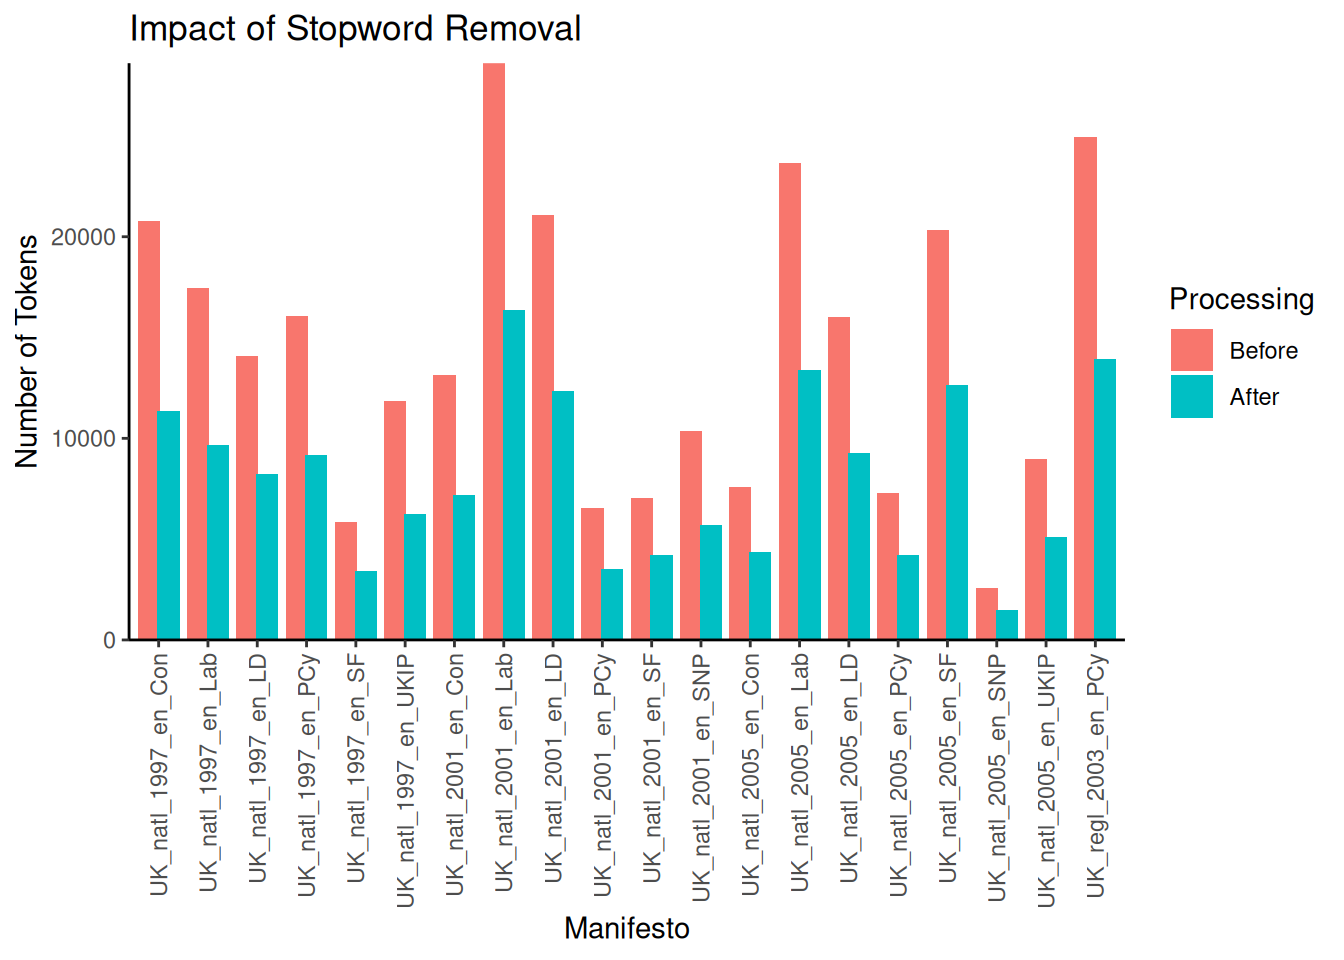
\includegraphics[keepaspectratio]{Introduction-to-Quantitative-Text-Analysis_files/figure-latex/ggplot-stopwords-impact-1.pdf}}

As expected, removing stopwords substantially reduces the total number of tokens across all documents. The number of words removed differs per document but can be substantial, for example, in the case of the 2001 Labour Party manifesto, which was reduced from \(28,606\) to \(16,386\) words --- a reduction of around \(42\%\). Finally, remember that \texttt{stopwords("english")} is nothing more than a character vector of stop words. Therefore, if we wish to remove stop words ourselves, we can do so by simply providing them as such:

\begin{Shaded}
\begin{Highlighting}[]
\NormalTok{data\_tokens\_nostop }\OtherTok{\textless{}{-}}\NormalTok{ quanteda}\SpecialCharTok{::}\FunctionTok{tokens\_select}\NormalTok{(data\_tokens\_nostop, }\FunctionTok{c}\NormalTok{(}\StringTok{"may"}\NormalTok{, }\StringTok{"new"}\NormalTok{,}
    \StringTok{"manifesto"}\NormalTok{), }\AttributeTok{selection =} \StringTok{"remove"}\NormalTok{, }\AttributeTok{valuetype =} \StringTok{"fixed"}\NormalTok{)}
\end{Highlighting}
\end{Shaded}

\subsection{N-grams and Collocations}\label{n-grams-and-collocations}

While individual words (unigrams) are the most common features in text analysis, sometimes the meaning is better captured by sequences of words, known as \textbf{n-grams}. An n-gram is a contiguous sequence of \emph{n} items from a given sample of text or speech. For example, ``strong economy'' is a 2-gram (or bigram), and ``peace and prosperity'' is a 3-gram (or trigram). Using n-grams can help us to capture phrases, multi-word expressions, and local context that single words miss. The \texttt{quanteda} package provides \texttt{tokens\_ngrams()} to generate all possible n-grams of a specified size from a tokens object. Here, \texttt{\#\ n\ =\ 2} specifies bigrams:

\begin{Shaded}
\begin{Highlighting}[]
\NormalTok{data\_tokens\_bigrams }\OtherTok{\textless{}{-}} \FunctionTok{tokens\_ngrams}\NormalTok{(data\_tokens\_nostop, }\AttributeTok{n =} \DecValTok{2}\NormalTok{)}
\FunctionTok{head}\NormalTok{(data\_tokens\_bigrams[[}\DecValTok{5}\NormalTok{]], }\DecValTok{10}\NormalTok{)}
\end{Highlighting}
\end{Shaded}

\begin{verbatim}
##  [1] "contents_opportunity" "opportunity_peace"    "peace_unionists"     
##  [4] "unionists_economy"    "economy_social"       "social_justice"      
##  [7] "justice_economic"     "economic_equality"    "equality_young"      
## [10] "young_people's"
\end{verbatim}

While \texttt{tokens\_ngrams()} can generate n-grams, the problem is that it creates \emph{all} possible numbers of n-grams, many of which are not meaningful or useful (such as `opportunity\_peace'). Therefore, it is a better idea first to identify \textbf{collocations} -- n-grams that appear more frequently than we would expect by chance. These often represent meaningful phrases or concepts (for example, given that we are working with UK manifestos, we would expect combinations such as ``Prime Minister'' or ``National Health Service''). We can identify these with the \texttt{textstat\_collocations()} function, which calculates various association measures (like likelihood ratio, PMI, and chi-squared) to score potential collocations. Depending on your analysis, you might calculate collocations before stopword removal if you think that stopwords could be part of a collocation you would like to capture (for instance, if you are interested in capturing the term ``we the people''). For this example, we will look for collocations after the stopwords are removed. Here, \texttt{\#\ min\_count} specifies the minimum number of times a collocation must appear to be considered. The standard (\(2\)) thus means that a combination appears more than a single time, and is thus not a random combination. Here we set ours at \(5\):

\begin{Shaded}
\begin{Highlighting}[]
\NormalTok{collocations }\OtherTok{\textless{}{-}} \FunctionTok{textstat\_collocations}\NormalTok{(data\_tokens\_nostop, }\AttributeTok{min\_count =} \DecValTok{5}\NormalTok{, }\AttributeTok{size =} \DecValTok{2}\NormalTok{)}
\end{Highlighting}
\end{Shaded}

Now that we have found all the possible collocations, it is time to decide which ones we want to use. One aspect we can utilise for this is the Wald \(z\)-statistic, which calculates the likelihood that the two words would occur together at random. Here, we decide to include only those collocations with a \(z>3\), which means they are three standard errors away from the mean (and thus have a p-value of approximately \(0.0027\)) of being likely:

\begin{Shaded}
\begin{Highlighting}[]
\NormalTok{collocations }\OtherTok{\textless{}{-}}\NormalTok{ collocations[collocations}\SpecialCharTok{$}\NormalTok{z }\SpecialCharTok{\textgreater{}} \DecValTok{3}\NormalTok{, ]}
\FunctionTok{head}\NormalTok{(collocations, }\DecValTok{20}\NormalTok{)}
\end{Highlighting}
\end{Shaded}

\begin{verbatim}
##                collocation count count_nested length   lambda        z
## 1        local authorities   145            0      2 6.227087 39.79911
## 2             young people   143            0      2 5.516777 39.77435
## 3           european union   114            0      2 7.258521 39.45265
## 4           health service    92            0      2 5.002104 37.77858
## 5          public services   105            0      2 4.125346 35.71296
## 6                long term    60            0      2 7.560533 35.69555
## 7               income tax    77            0      2 5.246884 35.28413
## 8              party wales    88            0      2 4.497066 34.41696
## 9         small businesses    52            0      2 6.810025 34.11001
## 10        public transport    77            0      2 4.700041 33.27666
## 11             council tax    68            0      2 5.103959 33.10773
## 12          private sector    51            0      2 5.603853 31.87116
## 13             cymru party    55            0      2 5.169383 31.42865
## 14            labour party    69            0      2 4.471125 31.34627
## 15            human rights    85            0      2 7.954503 30.72153
## 16                per year    58            0      2 4.732218 30.50192
## 17             rural areas    52            0      2 5.087455 30.47553
## 18 conservative government    74            0      2 4.876933 30.34761
## 19         next parliament    49            0      2 5.395004 30.31724
## 20           waiting times    39            0      2 8.122568 30.24217
\end{verbatim}

As we can see, we now capture some relevant combinations such as ``european union'', ``local authorities'', and ``income tax''. We could remove all the terms we do not wish to from the data frame, but we will leave this for now. For now, we will ``compound'' them using \texttt{tokens\_compound()}. This function replaces the sequence of individual tokens that form a collocation with a single, multi-word token (e.g., ``national\_health\_service''). This ensures that the identified phrase is treated as a single feature from now on (as both the tokens object and the DFM will see \texttt{\_} as the sign for a compound):

\begin{Shaded}
\begin{Highlighting}[]
\NormalTok{data\_tokens\_compounded }\OtherTok{\textless{}{-}} \FunctionTok{tokens\_compound}\NormalTok{(data\_tokens\_nostop, }\AttributeTok{pattern =}\NormalTok{ collocations,}
    \AttributeTok{concatenator =} \StringTok{"\_"}\NormalTok{)}
\FunctionTok{head}\NormalTok{(data\_tokens\_compounded[[}\DecValTok{5}\NormalTok{]], }\DecValTok{10}\NormalTok{)}
\end{Highlighting}
\end{Shaded}

\begin{verbatim}
##  [1] "contents"       "opportunity"    "peace"          "unionists"     
##  [5] "economy"        "social_justice" "economic"       "equality"      
##  [9] "young_people's" "rights"
\end{verbatim}

Note that now the words ``social justice'' are combined into a single new term. Also, note that while we mainly calculate the collocations after initial lowercasing and punctuation removal, whether we do so before or after stopword removal and stemming depends on whether we see the stopwords and word endings as part of the collocation. For instance, stemming ``social security'' to ``social secur'' might be desired, but stemming before identifying the collocation could make it harder for us to identify the collocation.

\subsection{Stemming and Lemmatisation}\label{stemming-and-lemmatisation}

Stemming and lemmatisation are two techniques that reduce words to a common form, to group variations (e.g., ``run'', ``running'', ``ran''). This can help us to treat words with similar meanings as equivalent features, reducing the overall vocabulary size and improving the signal-to-noise ratio in the data.

\emph{Stemming} uses algorithmic rules to chop off suffixes (and sometimes prefixes) from words, often resulting in a truncated ``stem'' that may not be a real word (e.g., ``university'' -\textgreater{} ``univers'', ``connection'' -\textgreater{} ``connect''). \texttt{quanteda} provides the \texttt{tokens\_wordstem()} function, which uses the Porter stemmer by default for English. While fast, stemming can sometimes produce non-words or conflate words with different meanings.

\emph{Lemmatisation} is a more linguistically informed process that uses a lexicon (a dictionary of words and their base forms) to convert words to their dictionary form, or \emph{lemma} (e.g., ``better'' -\textgreater{} ``good'', ``geese'' -\textgreater{} ``goose'', ``running'' -\textgreater{} ``run''). Lemmatisation generally produces valid words. It can be more accurate than stemming but typically requires external resources, such as lexicons. Also, it is computationally more intensive. \texttt{quanteda} does not have a built-in lemmatiser. Still, you can perform lemmatisation before creating a \texttt{corpus} or \texttt{tokens} object using other R packages (like \texttt{textstem} or \texttt{spacyr}).

Here, we will do some stemming using \texttt{tokens\_wordstem()}:

\begin{Shaded}
\begin{Highlighting}[]
\NormalTok{data\_tokens\_stemmed }\OtherTok{\textless{}{-}} \FunctionTok{tokens\_wordstem}\NormalTok{(data\_tokens\_compounded, }\AttributeTok{language =} \StringTok{"english"}\NormalTok{)}
\FunctionTok{head}\NormalTok{(data\_tokens\_stemmed[[}\DecValTok{5}\NormalTok{]], }\DecValTok{20}\NormalTok{)}
\end{Highlighting}
\end{Shaded}

\begin{verbatim}
##  [1] "content"                "opportun"               "peac"                  
##  [4] "unionist"               "economi"                "social_justic"         
##  [7] "econom"                 "equal"                  "young_peopl"           
## [10] "right"                  "education_train"        "farming_rural_develop" 
## [13] "environ"                "cultur"                 "women"                 
## [16] "irish_political_prison" "polic"                  "futur"                 
## [19] "opportun"               "peac"
\end{verbatim}

Note how words like ``economy'', ``culture'', and ``peace'' have been reduced to their stems (``economi'', ``cultur'', ``peac''). As before, let's visualise this as well:

\begin{Shaded}
\begin{Highlighting}[]
\CommentTok{\# Calculate the number of types (unique tokens)}

\NormalTok{types\_before\_stem }\OtherTok{\textless{}{-}} \FunctionTok{ntype}\NormalTok{(data\_tokens\_compounded)}
\NormalTok{types\_after\_stem }\OtherTok{\textless{}{-}} \FunctionTok{ntype}\NormalTok{(data\_tokens\_stemmed)}

\NormalTok{stemming\_data }\OtherTok{\textless{}{-}} \FunctionTok{data.frame}\NormalTok{(}
  \AttributeTok{document =} \FunctionTok{docnames}\NormalTok{(data\_tokens\_nostop),}
  \CommentTok{\# Get document names}
  \AttributeTok{Before =}\NormalTok{ types\_before\_stem,}
  \AttributeTok{After =}\NormalTok{ types\_after\_stem}
\NormalTok{)}

\NormalTok{stemming\_data }\OtherTok{\textless{}{-}} \FunctionTok{melt}\NormalTok{(}
\NormalTok{  stemming\_data,}
  \AttributeTok{id.vars =} \StringTok{"document"}\NormalTok{,}
  \AttributeTok{variable.name =} \StringTok{"Processing"}\NormalTok{,}
  \AttributeTok{value.name =} \StringTok{"NumTypes"}
\NormalTok{)}

\CommentTok{\# Create a bar plot comparing each document\textquotesingle{}s type counts before and after stemming}

\FunctionTok{ggplot}\NormalTok{(stemming\_data, }\FunctionTok{aes}\NormalTok{(}\AttributeTok{x =}\NormalTok{ document, }\AttributeTok{y =}\NormalTok{ NumTypes, }\AttributeTok{fill =}\NormalTok{ Processing)) }\SpecialCharTok{+}
  \FunctionTok{geom\_bar}\NormalTok{(}\AttributeTok{stat =} \StringTok{"identity"}\NormalTok{, }\AttributeTok{position =} \FunctionTok{position\_dodge}\NormalTok{(}\AttributeTok{width =} \FloatTok{0.8}\NormalTok{)) }\SpecialCharTok{+} \CommentTok{\# Use dodged bars.}
  \FunctionTok{scale\_x\_discrete}\NormalTok{(}\AttributeTok{name =} \StringTok{"Manifesto"}\NormalTok{) }\SpecialCharTok{+}
  \FunctionTok{scale\_y\_continuous}\NormalTok{(}\AttributeTok{name =} \StringTok{"Number of Tokens"}\NormalTok{, }\AttributeTok{expand =} \FunctionTok{c}\NormalTok{(}\DecValTok{0}\NormalTok{, }\DecValTok{0}\NormalTok{)) }\SpecialCharTok{+}
  \FunctionTok{ggtitle}\NormalTok{(}\StringTok{"Impact of Stemming"}\NormalTok{) }\SpecialCharTok{+}
  \FunctionTok{theme\_classic}\NormalTok{() }\SpecialCharTok{+}
  \FunctionTok{theme}\NormalTok{(}\AttributeTok{axis.text.x =} \FunctionTok{element\_text}\NormalTok{(}
    \AttributeTok{angle =} \DecValTok{90}\NormalTok{,}
    \AttributeTok{vjust =} \FloatTok{0.5}\NormalTok{,}
    \AttributeTok{hjust =} \DecValTok{1}
\NormalTok{  ))  }\CommentTok{\# Rotate x{-}axis labels}
\end{Highlighting}
\end{Shaded}

\pandocbounded{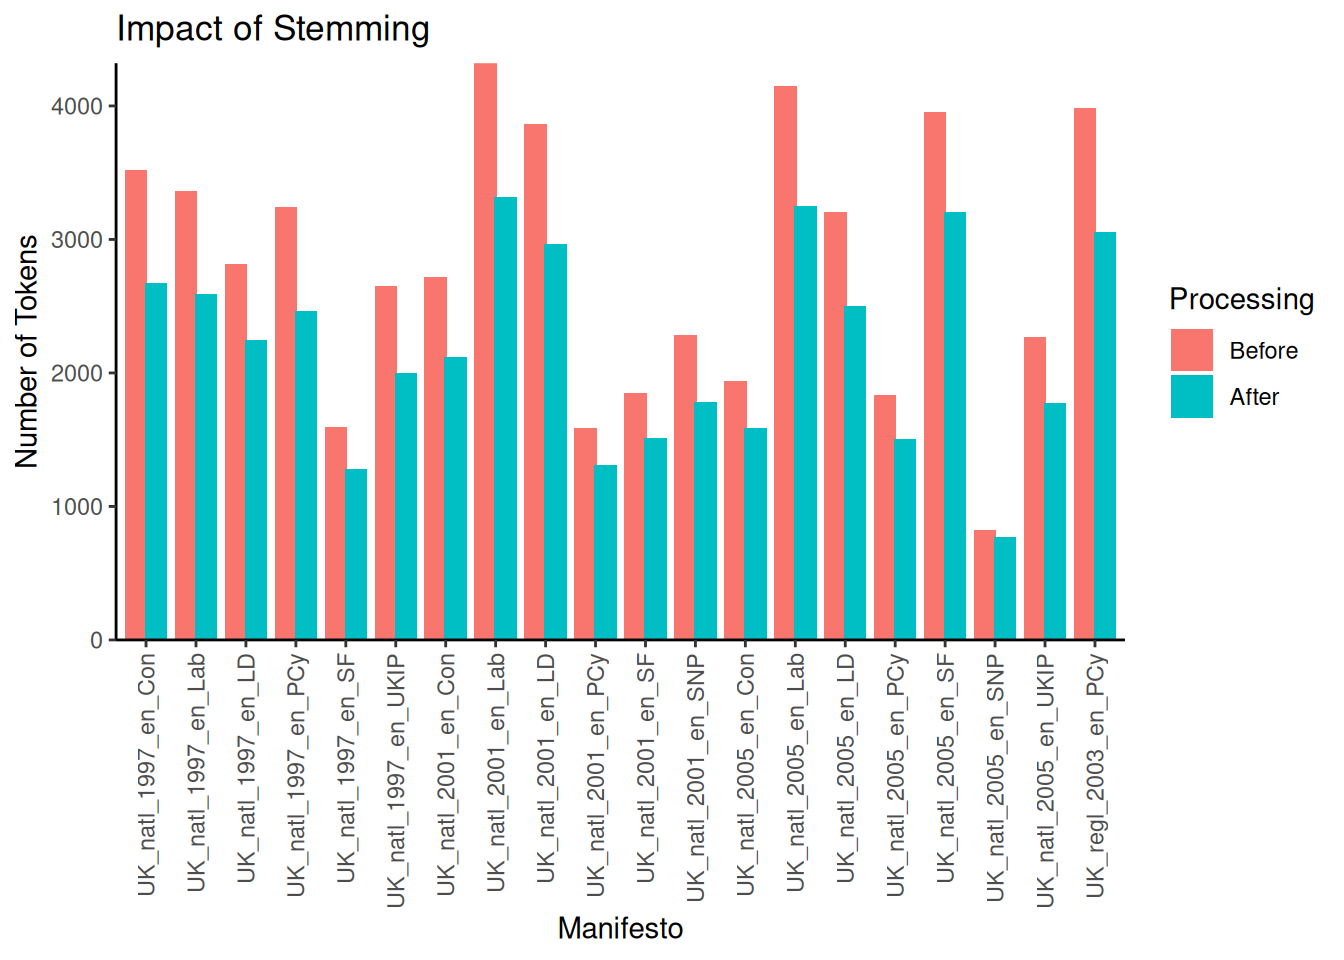
\includegraphics[keepaspectratio]{Introduction-to-Quantitative-Text-Analysis_files/figure-latex/ggplot-stemming-impact-1.pdf}}

Again, removing the words from their stems can remove a significant number of unique features. For example, looking at the 2001 Labour manifesto shows that from the \(4320\) types before stemming, only \(3315\) remained afterwards.

\subsection{Removing Sparse Features (DFM Trimming)}\label{removing-sparse-features-dfm-trimming}

After tokenisation and linguistic pre-processing, we can generate our DFM. However, at this point, our DFM might still contain many features (terms) that appear infrequently across the corpus or in only a few documents. These \emph{sparse features} can increase the dimensionality of our data without adding much useful information and can sometimes be noise (e.g., typos). Removing them can decrease processing time and also the performance of some models. We can use the \texttt{dfm\_trim()} function for DFM trimming. We can set thresholds based on minimum term frequency (\texttt{min\_termfreq}), maximum term frequency (\texttt{max\_termfreq}), minimum document frequency (\texttt{min\_docfreq}), or maximum document frequency (\texttt{max\_docfreq}), either as absolute counts or percentages:

\begin{Shaded}
\begin{Highlighting}[]
\NormalTok{data\_dfm\_untrimmed }\OtherTok{\textless{}{-}} \FunctionTok{dfm}\NormalTok{(data\_tokens\_stemmed)}
\NormalTok{data\_dfm\_trimmed }\OtherTok{\textless{}{-}} \FunctionTok{dfm\_trim}\NormalTok{(data\_dfm\_untrimmed, }\AttributeTok{min\_docfreq =} \DecValTok{2}\NormalTok{)  }\CommentTok{\# Trim the dfm to remove features that appear in fewer than two documents}

\CommentTok{\# You could also trim by minimum term frequency (total occurrences across the}
\CommentTok{\# corpus): data\_dfm\_trimmed\_freq \textless{}{-} dfm\_trim(data\_dfm\_untrimmed, min\_termfreq =}
\CommentTok{\# 10)}

\NormalTok{data\_dfm\_untrimmed}
\end{Highlighting}
\end{Shaded}

\begin{verbatim}
## Document-feature matrix of: 20 documents, 11,789 features (81.37% sparse) and 6 docvars.
##                       features
## docs                   conserv foreword administr elect sinc among success
##   UK_natl_1997_en_Con       19        1         3     7   28     3      29
##   UK_natl_1997_en_Lab       43        0         8    15    4     7      19
##   UK_natl_1997_en_LD         2        0         2    12    0     0       4
##   UK_natl_1997_en_PCy        1        1         2     6    0     5       8
##   UK_natl_1997_en_SF         0        0         2     6    5     1       3
##   UK_natl_1997_en_UKIP       3        0         4     8    6     1       6
##                       features
## docs                   british peacetim histori
##   UK_natl_1997_en_Con       32        1       8
##   UK_natl_1997_en_Lab       19        2       7
##   UK_natl_1997_en_LD         6        0       0
##   UK_natl_1997_en_PCy        7        0       3
##   UK_natl_1997_en_SF         9        0       2
##   UK_natl_1997_en_UKIP       2        0       3
## [ reached max_ndoc ... 14 more documents, reached max_nfeat ... 11,779 more features ]
\end{verbatim}

\begin{Shaded}
\begin{Highlighting}[]
\NormalTok{data\_dfm\_trimmed}
\end{Highlighting}
\end{Shaded}

\begin{verbatim}
## Document-feature matrix of: 20 documents, 6,257 features (69.33% sparse) and 6 docvars.
##                       features
## docs                   conserv foreword administr elect sinc among success
##   UK_natl_1997_en_Con       19        1         3     7   28     3      29
##   UK_natl_1997_en_Lab       43        0         8    15    4     7      19
##   UK_natl_1997_en_LD         2        0         2    12    0     0       4
##   UK_natl_1997_en_PCy        1        1         2     6    0     5       8
##   UK_natl_1997_en_SF         0        0         2     6    5     1       3
##   UK_natl_1997_en_UKIP       3        0         4     8    6     1       6
##                       features
## docs                   british peacetim histori
##   UK_natl_1997_en_Con       32        1       8
##   UK_natl_1997_en_Lab       19        2       7
##   UK_natl_1997_en_LD         6        0       0
##   UK_natl_1997_en_PCy        7        0       3
##   UK_natl_1997_en_SF         9        0       2
##   UK_natl_1997_en_UKIP       2        0       3
## [ reached max_ndoc ... 14 more documents, reached max_nfeat ... 6,247 more features ]
\end{verbatim}

Note that when we trim the DFM to remove features that appear in fewer than five documents, we reduce the sparsity (i.e., empty cells in the DFM) from \(81.37\%\) to \(69.33\%\). We also go from \(11,789\) for features (types) to \(6,257\). Trimming significantly reduces the number of features in the DFM by removing those that occur very rarely. The specific thresholds you choose for trimming will depend on the size of your corpus, the nature of your text, and your analytical goals. One reason to use it (and why we set it to \(2\) here) is that `unique' words are rarely very interesting. Besides, removing words that occur only a single time can be a good way of removing spelling mistakes. However, be mindful that overly aggressive trimming can remove potentially informative rare terms.

\subsection{Additional Pre-Processing}\label{additional-pre-processing}

Besides using the functions built into \texttt{quanteda}, we can also use R's more native functions to clean texts. For this, we have to clean our text while it is still in a data frame. There are several ways to do this, including R's \texttt{gsub}. However, we will use the more powerful and faster \texttt{stringr} package, part of the \texttt{tidyverse}, here. To use \texttt{stringr}, we first need to load the library. We must also ensure that our texts are stored as a data frame. For demonstration purposes here, we will take our original (and non-pre-processed) corpus and make it into a data frame using the \texttt{convert} function:

\begin{Shaded}
\begin{Highlighting}[]
\FunctionTok{library}\NormalTok{(stringr)}
\NormalTok{data\_corpus\_df }\OtherTok{\textless{}{-}} \FunctionTok{convert}\NormalTok{(data\_corpus\_ukmanifestos, }\AttributeTok{to =} \StringTok{"data.frame"}\NormalTok{)}
\end{Highlighting}
\end{Shaded}

Now we can use \texttt{stringr} functions like \texttt{str\_replace\_all()} to clean up the text. \texttt{str\_replace\_all()} takes a character vector, a pattern to find and a replacement string. We will use regular expressions for the pattern.

\begin{Shaded}
\begin{Highlighting}[]
\CommentTok{\# Remove URLs (http, https, ftp, ftps)}
\NormalTok{data\_corpus\_df}\SpecialCharTok{$}\NormalTok{text }\OtherTok{\textless{}{-}} \FunctionTok{str\_replace\_all}\NormalTok{(data\_corpus\_df}\SpecialCharTok{$}\NormalTok{text, }\StringTok{"http[s]?://[\^{} ]+"}\NormalTok{, }\StringTok{""}\NormalTok{)}
\NormalTok{data\_corpus\_df}\SpecialCharTok{$}\NormalTok{text }\OtherTok{\textless{}{-}} \FunctionTok{str\_replace\_all}\NormalTok{(data\_corpus\_df}\SpecialCharTok{$}\NormalTok{text, }\StringTok{"ftp[s]?://[\^{} ]+"}\NormalTok{, }\StringTok{""}\NormalTok{)  }\CommentTok{\# Also include ftp/s}

\CommentTok{\# Remove mentions (@username)}
\NormalTok{data\_corpus\_df}\SpecialCharTok{$}\NormalTok{text }\OtherTok{\textless{}{-}} \FunctionTok{str\_replace\_all}\NormalTok{(data\_corpus\_df}\SpecialCharTok{$}\NormalTok{text, }\StringTok{"@}\SpecialCharTok{\textbackslash{}\textbackslash{}}\StringTok{w+"}\NormalTok{, }\StringTok{""}\NormalTok{)}

\CommentTok{\# Remove hashtags (\#topic) {-} keep the topic word, remove the \#}
\NormalTok{data\_corpus\_df}\SpecialCharTok{$}\NormalTok{text }\OtherTok{\textless{}{-}} \FunctionTok{str\_replace\_all}\NormalTok{(data\_corpus\_df}\SpecialCharTok{$}\NormalTok{text, }\StringTok{"\#(}\SpecialCharTok{\textbackslash{}\textbackslash{}}\StringTok{w+)"}\NormalTok{, }\StringTok{"}\SpecialCharTok{\textbackslash{}\textbackslash{}}\StringTok{1"}\NormalTok{)}

\CommentTok{\# Remove punctuation}
\NormalTok{data\_corpus\_df}\SpecialCharTok{$}\NormalTok{text }\OtherTok{\textless{}{-}} \FunctionTok{str\_replace\_all}\NormalTok{(data\_corpus\_df}\SpecialCharTok{$}\NormalTok{text, }\StringTok{"[[:punct:]]"}\NormalTok{, }\StringTok{""}\NormalTok{)}

\CommentTok{\# Remove numbers (optional, depending on analysis)}
\NormalTok{data\_corpus\_df}\SpecialCharTok{$}\NormalTok{text }\OtherTok{\textless{}{-}} \FunctionTok{str\_replace\_all}\NormalTok{(data\_corpus\_df}\SpecialCharTok{$}\NormalTok{text, }\StringTok{"[[:digit:]]"}\NormalTok{, }\StringTok{""}\NormalTok{)}

\CommentTok{\# Remove retweet indicator \textquotesingle{}RT\textquotesingle{} (ensure it\textquotesingle{}s at the start of a potential tweet)}
\NormalTok{data\_corpus\_df}\SpecialCharTok{$}\NormalTok{text }\OtherTok{\textless{}{-}} \FunctionTok{str\_replace\_all}\NormalTok{(data\_corpus\_df}\SpecialCharTok{$}\NormalTok{text, }\StringTok{"\^{}RT}\SpecialCharTok{\textbackslash{}\textbackslash{}}\StringTok{s"}\NormalTok{, }\StringTok{""}\NormalTok{)  }\CommentTok{\# Use \^{}RT\textbackslash{}\textbackslash{}s to match RT at the start followed by space}

\CommentTok{\# Remove extra whitespace (leading, trailing, and multiple spaces)}
\NormalTok{data\_corpus\_df}\SpecialCharTok{$}\NormalTok{text }\OtherTok{\textless{}{-}} \FunctionTok{str\_trim}\NormalTok{(data\_corpus\_df}\SpecialCharTok{$}\NormalTok{text)  }\CommentTok{\# Remove leading/trailing whitespace using str\_trim}
\NormalTok{data\_corpus\_df}\SpecialCharTok{$}\NormalTok{text }\OtherTok{\textless{}{-}} \FunctionTok{str\_replace\_all}\NormalTok{(data\_corpus\_df}\SpecialCharTok{$}\NormalTok{text, }\StringTok{"[[:space:]]\{2,\}"}\NormalTok{, }\StringTok{" "}\NormalTok{)  }\CommentTok{\# Replace multiple spaces with a single space}

\CommentTok{\# Convert to lower{-}case (important for dictionary matching)}
\NormalTok{data\_corpus\_df}\SpecialCharTok{$}\NormalTok{text }\OtherTok{\textless{}{-}} \FunctionTok{str\_to\_lower}\NormalTok{(data\_corpus\_df}\SpecialCharTok{$}\NormalTok{text)}
\end{Highlighting}
\end{Shaded}

Note that in most cases, the functions in \texttt{quanteda} are enough. However, \texttt{str\_replace\_all()} can be practical before regular pre-processing, especially when dealing with problematic data.

\subsection{Evaluating Pre-Processing}\label{evaluating-pre-processing}

The selection and order of these pre-processing steps can substantially impact the resulting DFM and, as a result, the outcomes of your text analysis. For example:

\begin{itemize}
\tightlist
\item
  Removing stopwords might remove terms that are crucial in a specific context or field
\item
  Stemming can group words that have different meanings (e.g., ``organ'' and ``organise'')
\item
  The order of removing stopwords before or after calculating collocations affects the collocations we find
\end{itemize}

In other words, simply pre-processing our data can lead to different data sets and, therefore, to different conclusions later on during our analysis. To see what effect our pre-processing decisions had, we can use the \texttt{preText} package by Denny \& Spirling (\citeproc{ref-Denny2018a}{2018}) to see what the impact of each step is on our analysis. \texttt{preText} works by applying all of the different possible combinations of pre-processing steps (7 in total, leading to 2⁷ = 128 possible combinations) to your corpus and then comparing the similarities between the different DFMs.

First, ensure the \texttt{preText} package is installed and loaded:

\begin{Shaded}
\begin{Highlighting}[]
\FunctionTok{library}\NormalTok{(preText)}
\FunctionTok{library}\NormalTok{(reshape2)}
\end{Highlighting}
\end{Shaded}

First, we run \texttt{factorial\_preprocessing()}, which takes a corpus object (or other text formats) and applies a set of default pre-processing pipelines by systematically varying common pre-processing options. After this, we run the main \texttt{preText} command:

\begin{Shaded}
\begin{Highlighting}[]
\CommentTok{\# use\_ngrams = TRUE: Also consider including n{-}grams (sequences of words)}
\CommentTok{\# infrequent\_term\_threshold = 0.01: Remove terms that appear in less than 1\% of}
\CommentTok{\# documents}

\NormalTok{preprocessed\_documents }\OtherTok{\textless{}{-}} \FunctionTok{factorial\_preprocessing}\NormalTok{(data\_corpus\_ukmanifestos, }\AttributeTok{use\_ngrams =} \ConstantTok{TRUE}\NormalTok{,}
    \AttributeTok{infrequent\_term\_threshold =} \FloatTok{0.01}\NormalTok{, }\AttributeTok{parallel =} \ConstantTok{FALSE}\NormalTok{, }\AttributeTok{cores =} \DecValTok{1}\NormalTok{, }\AttributeTok{return\_results =} \ConstantTok{TRUE}\NormalTok{,}
    \AttributeTok{verbose =} \ConstantTok{TRUE}  \CommentTok{\# Display progress and information}
\NormalTok{)}

\CommentTok{\# Run the preText analysis, which compares the different pre{-}processed versions}
\CommentTok{\# distance\_method = \textquotesingle{}cosine\textquotesingle{}: Method to calculate distance between document}
\CommentTok{\# representations num\_comparisons = 50: Number of random document pairs to}
\CommentTok{\# compare for robustness}

\NormalTok{preText\_results }\OtherTok{\textless{}{-}} \FunctionTok{preText}\NormalTok{(preprocessed\_documents, }\AttributeTok{dataset\_name =} \StringTok{"UK Manifestos"}\NormalTok{,}
    \AttributeTok{distance\_method =} \StringTok{"cosine"}\NormalTok{, }\AttributeTok{num\_comparisons =} \DecValTok{50}\NormalTok{, }\AttributeTok{verbose =} \ConstantTok{TRUE}\NormalTok{)}
\end{Highlighting}
\end{Shaded}

After running \texttt{preText}, we can visualise the results. Two commands are already part of the package and provide a good overview of the results:

\begin{Shaded}
\begin{Highlighting}[]
\FunctionTok{preText\_score\_plot}\NormalTok{(preText\_results)}
\end{Highlighting}
\end{Shaded}

\pandocbounded{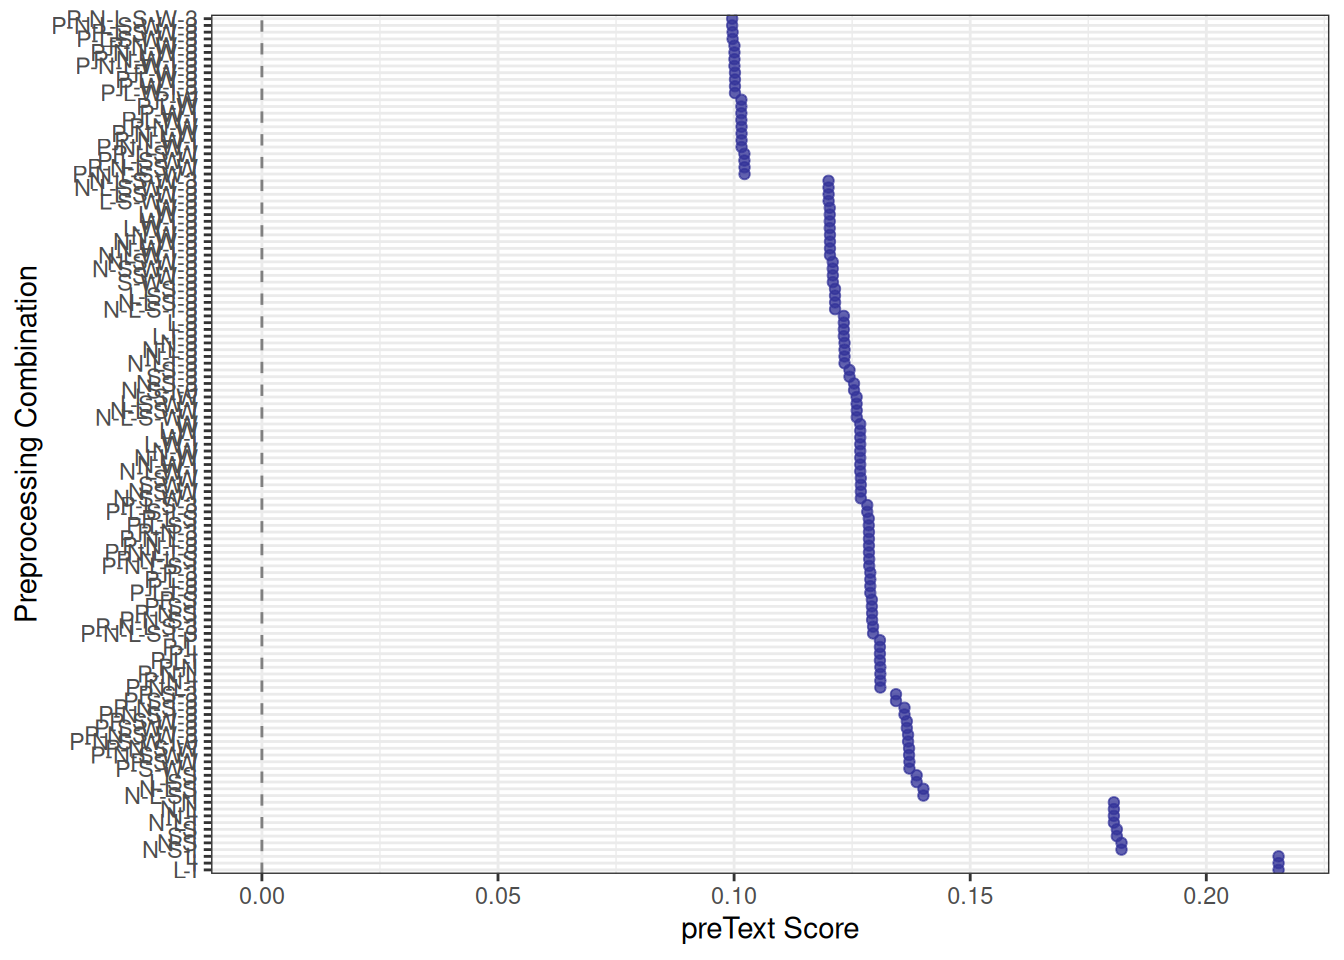
\includegraphics[keepaspectratio]{Introduction-to-Quantitative-Text-Analysis_files/figure-latex/pretext-models-1.pdf}}

\begin{Shaded}
\begin{Highlighting}[]
\FunctionTok{regression\_coefficient\_plot}\NormalTok{(preText\_results, }\AttributeTok{remove\_intercept =} \ConstantTok{TRUE}\NormalTok{)}
\end{Highlighting}
\end{Shaded}

\pandocbounded{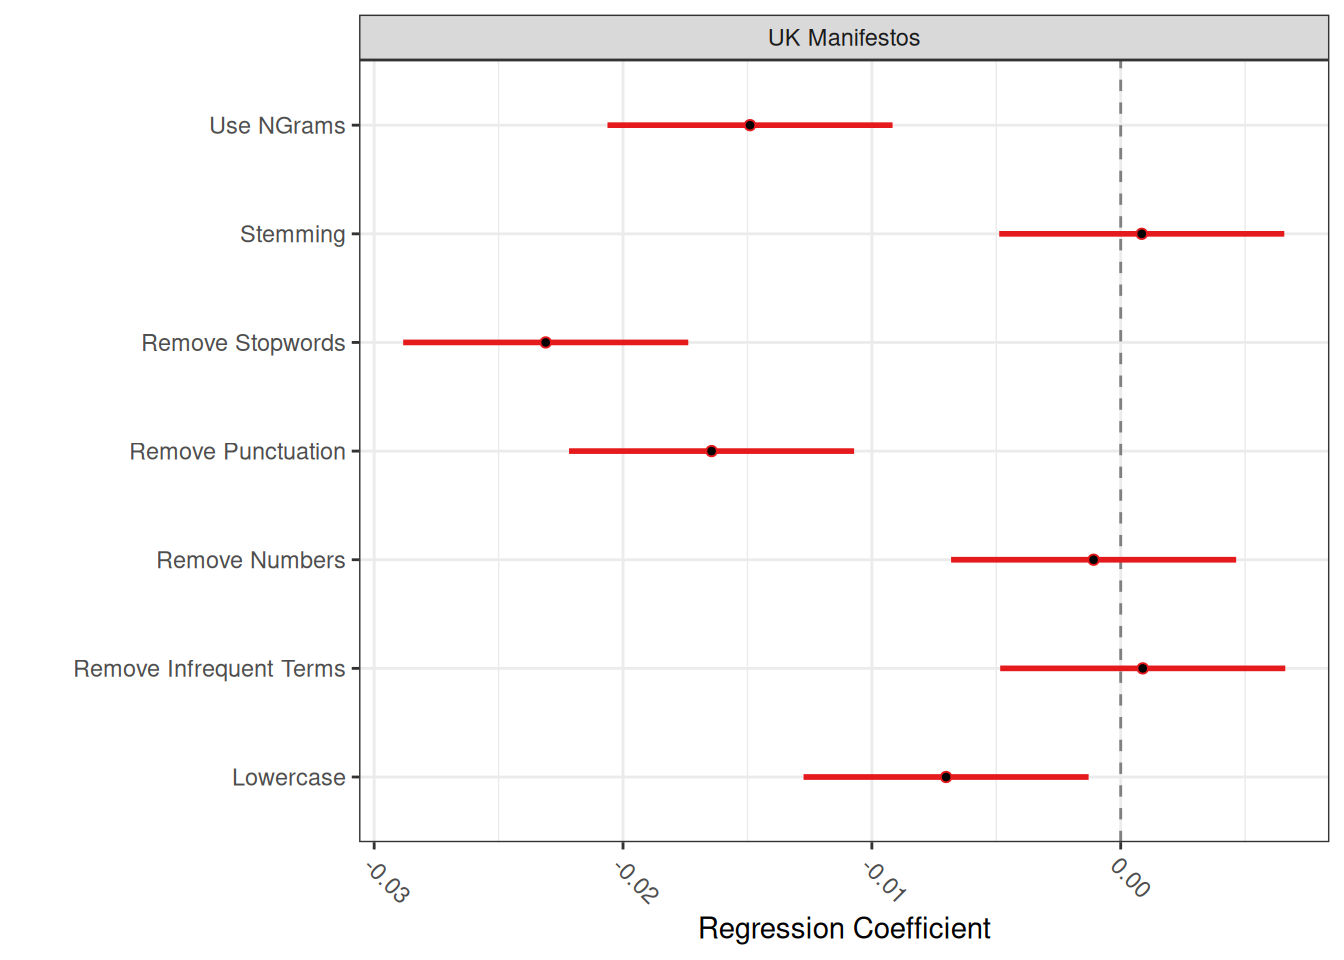
\includegraphics[keepaspectratio]{Introduction-to-Quantitative-Text-Analysis_files/figure-latex/pretext-models-2.pdf}}

In the first plot, lower scores indicate more robust pre-processing pipelines where document similarities are less sensitive to changes. In the second plot, which is the more interesting of the two, we are looking for pre-processing steps that are significantly different from the null line. In this case, this is the use of n-grams, the removal of stopwords and punctuation and lowercasing. The fact that they are different means that this pre-processing step has led to a significantly different DFM, which is, therefore, more likely to yield significantly different results in further analyses. Note that this does not say whether this is good or bad: we might still prefer a ``different'' and clean DFM over an uncleaned one. The point is that we are aware of these changes and should consider the potential impacts of our pre-processing on our subsequent analysis.

\section{Descriptives and Visualisations}\label{descriptives-and-visualisations}

Now that we have finished our DFM and assessed the effects of the pre-processing steps, it is time to examine our resulting DFM. For this, \texttt{quanteda} offers a variety of options. We start with a look at the most frequent tokens:

\begin{Shaded}
\begin{Highlighting}[]
\NormalTok{features }\OtherTok{\textless{}{-}} \FunctionTok{topfeatures}\NormalTok{(data\_dfm\_trimmed, }\DecValTok{50}\NormalTok{)  }\CommentTok{\# Get the top 50 most frequent features from the DFM}
\NormalTok{features\_plot }\OtherTok{\textless{}{-}} \FunctionTok{data.frame}\NormalTok{(}\AttributeTok{term =} \FunctionTok{names}\NormalTok{(features), }\AttributeTok{frequency =} \FunctionTok{unname}\NormalTok{(features))}

\NormalTok{features\_plot}\SpecialCharTok{$}\NormalTok{term }\OtherTok{\textless{}{-}} \FunctionTok{with}\NormalTok{(features\_plot, }\FunctionTok{reorder}\NormalTok{(term, }\SpecialCharTok{{-}}\NormalTok{frequency))  }\CommentTok{\# Reorder the terms by frequency in descending order}

\FunctionTok{ggplot}\NormalTok{(features\_plot, }\FunctionTok{aes}\NormalTok{(}\AttributeTok{x =}\NormalTok{ term, }\AttributeTok{y =}\NormalTok{ frequency)) }\SpecialCharTok{+} \FunctionTok{geom\_point}\NormalTok{() }\SpecialCharTok{+} \FunctionTok{theme\_classic}\NormalTok{() }\SpecialCharTok{+}
    \FunctionTok{scale\_x\_discrete}\NormalTok{(}\AttributeTok{name =} \StringTok{"Token"}\NormalTok{) }\SpecialCharTok{+} \FunctionTok{scale\_y\_continuous}\NormalTok{(}\AttributeTok{name =} \StringTok{"Frequency"}\NormalTok{) }\SpecialCharTok{+} \FunctionTok{ggtitle}\NormalTok{(}\StringTok{"Top 50 Most Frequent Tokens"}\NormalTok{) }\SpecialCharTok{+}
    \FunctionTok{theme}\NormalTok{(}\AttributeTok{axis.text.x =} \FunctionTok{element\_text}\NormalTok{(}\AttributeTok{angle =} \DecValTok{90}\NormalTok{, }\AttributeTok{hjust =} \DecValTok{1}\NormalTok{))}
\end{Highlighting}
\end{Shaded}

\pandocbounded{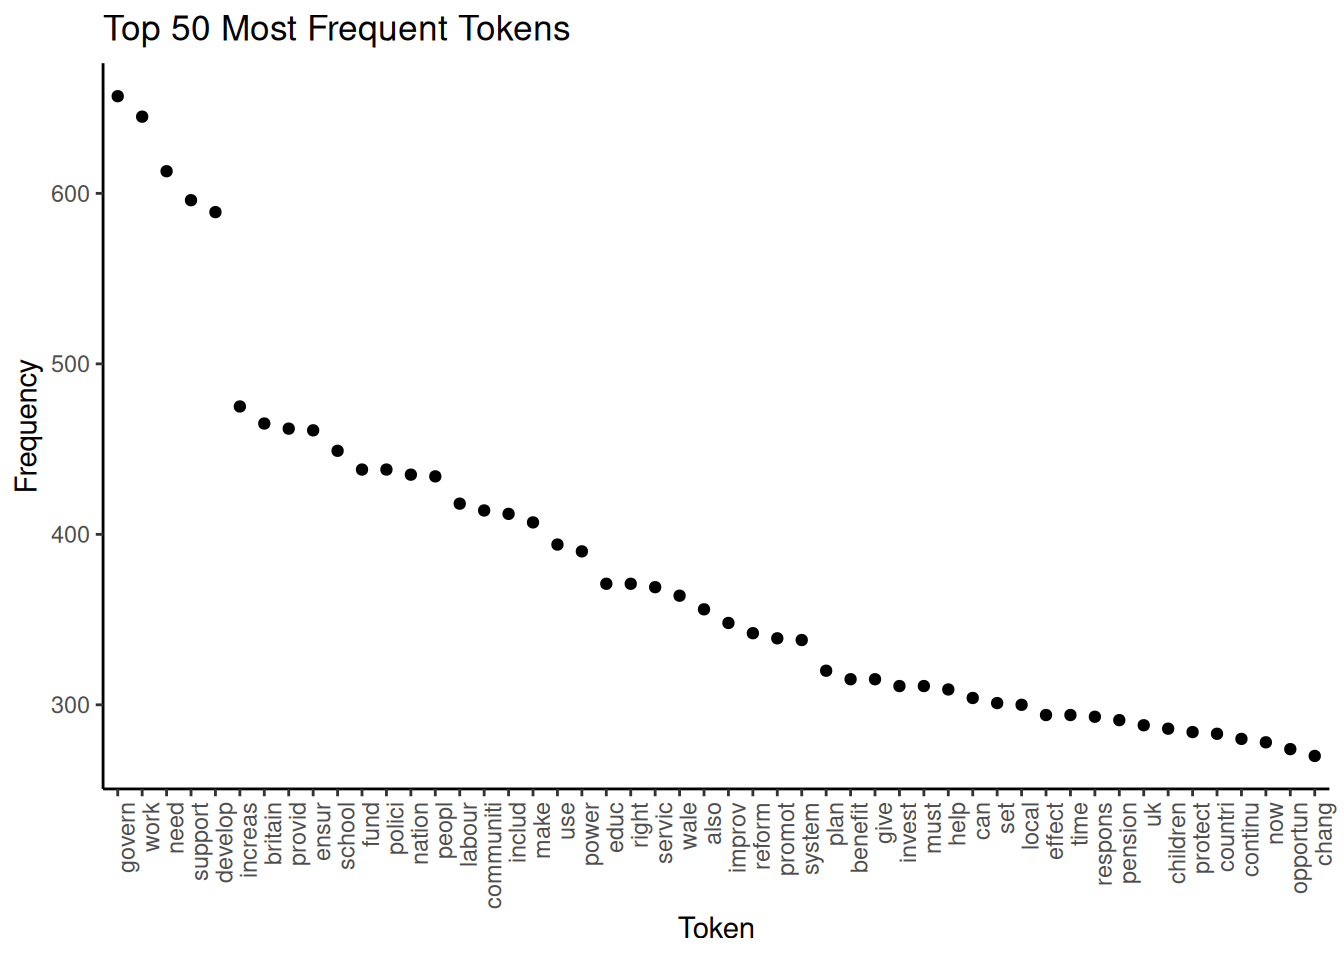
\includegraphics[keepaspectratio]{Introduction-to-Quantitative-Text-Analysis_files/figure-latex/topfeatures-manifesto-1.pdf}}
We can see that the words ``govern'', ``work'' and ``need'' are the most frequent, already indicating a little what our documents are about. Apart from this, a good use of a frequency graph is to spot stopwords you might wish to remove (for example, ``also'') and include them in the list of stopwords.

Another option for examining frequencies is to use word clouds. Not only are they a visually appealing way to visualise term frequencies, but word size also indicates frequency. While less precise than bar plots, we can use them for a quick impression of prominent terms. To avoid clutter, here, we include only terms that appear at least 20 times and set the maximum number of words in the word cloud at 100:

\begin{Shaded}
\begin{Highlighting}[]
\NormalTok{wordcloud\_dfm\_trim }\OtherTok{\textless{}{-}} \FunctionTok{dfm\_trim}\NormalTok{(data\_dfm\_trimmed, }\AttributeTok{min\_termfreq =} \DecValTok{20}\NormalTok{)}
\FunctionTok{textplot\_wordcloud}\NormalTok{(wordcloud\_dfm\_trim, }\AttributeTok{max\_words =} \DecValTok{100}\NormalTok{)}
\end{Highlighting}
\end{Shaded}

\pandocbounded{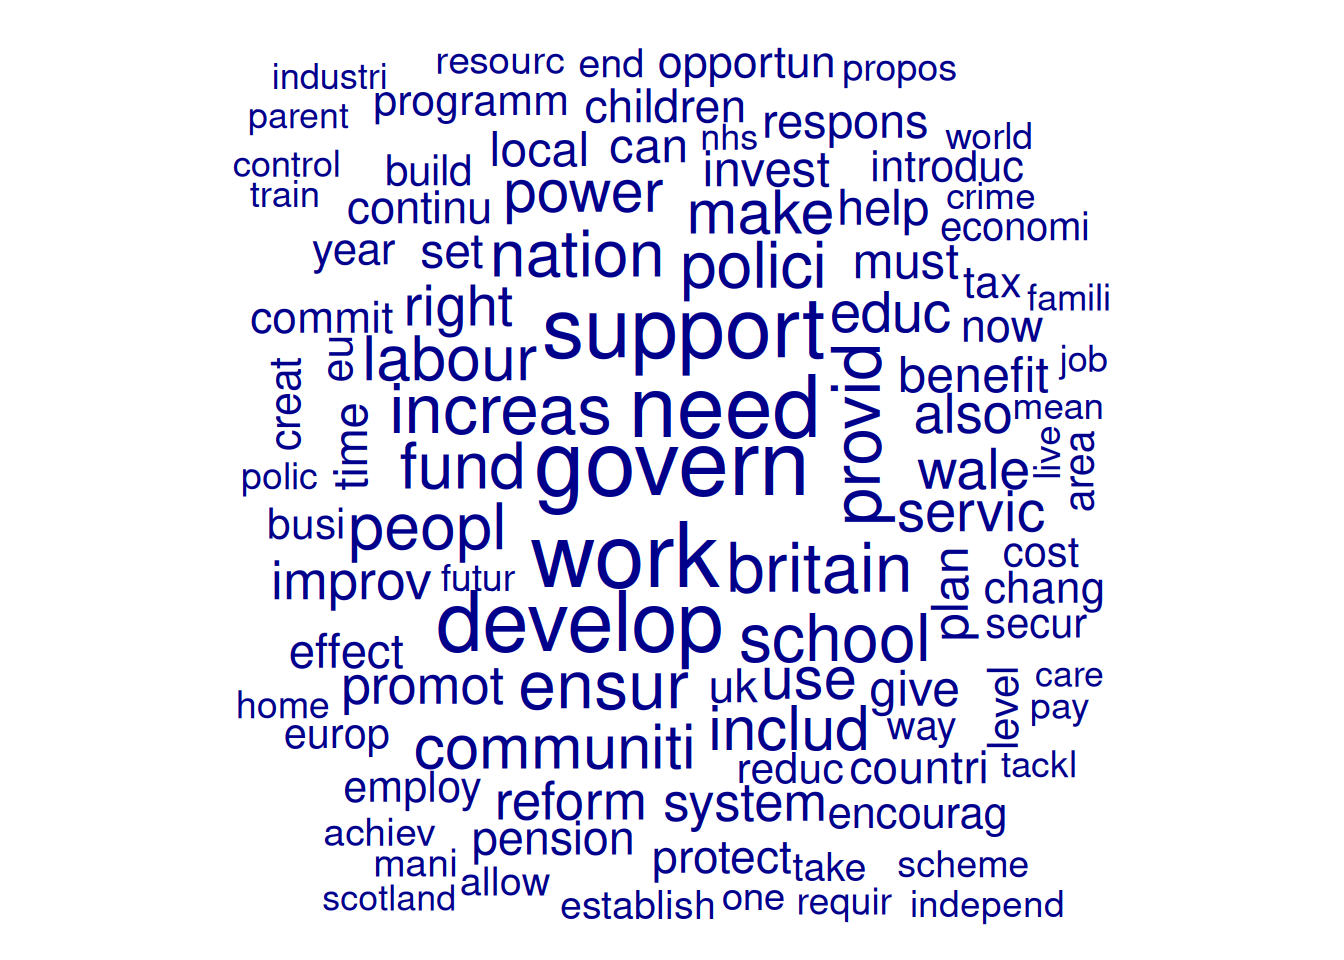
\includegraphics[keepaspectratio]{Introduction-to-Quantitative-Text-Analysis_files/figure-latex/wordcloud-manifesto-1.pdf}}

We can also compare docvars. Here, we first subset the DFM to include only Labour and Conservative manifestoes. Then we group them and then set \texttt{compare\ =\ TRUE}:

\begin{Shaded}
\begin{Highlighting}[]
\NormalTok{data\_dfm\_compare }\OtherTok{\textless{}{-}} \FunctionTok{dfm\_subset}\NormalTok{(data\_dfm\_trimmed, Party }\SpecialCharTok{\%in\%} \FunctionTok{c}\NormalTok{(}\StringTok{"Lab"}\NormalTok{, }\StringTok{"Con"}\NormalTok{))}
\NormalTok{wordcloud\_dfm\_trim }\OtherTok{\textless{}{-}} \FunctionTok{dfm\_group}\NormalTok{(data\_dfm\_compare, data\_dfm\_compare}\SpecialCharTok{$}\NormalTok{Party)}

\FunctionTok{textplot\_wordcloud}\NormalTok{(wordcloud\_dfm\_trim, }\AttributeTok{comparison =} \ConstantTok{TRUE}\NormalTok{, }\AttributeTok{max\_words =} \DecValTok{200}\NormalTok{, }\AttributeTok{color =} \FunctionTok{c}\NormalTok{(}\StringTok{"darkblue"}\NormalTok{,}
    \StringTok{"darkred"}\NormalTok{))}
\end{Highlighting}
\end{Shaded}

\pandocbounded{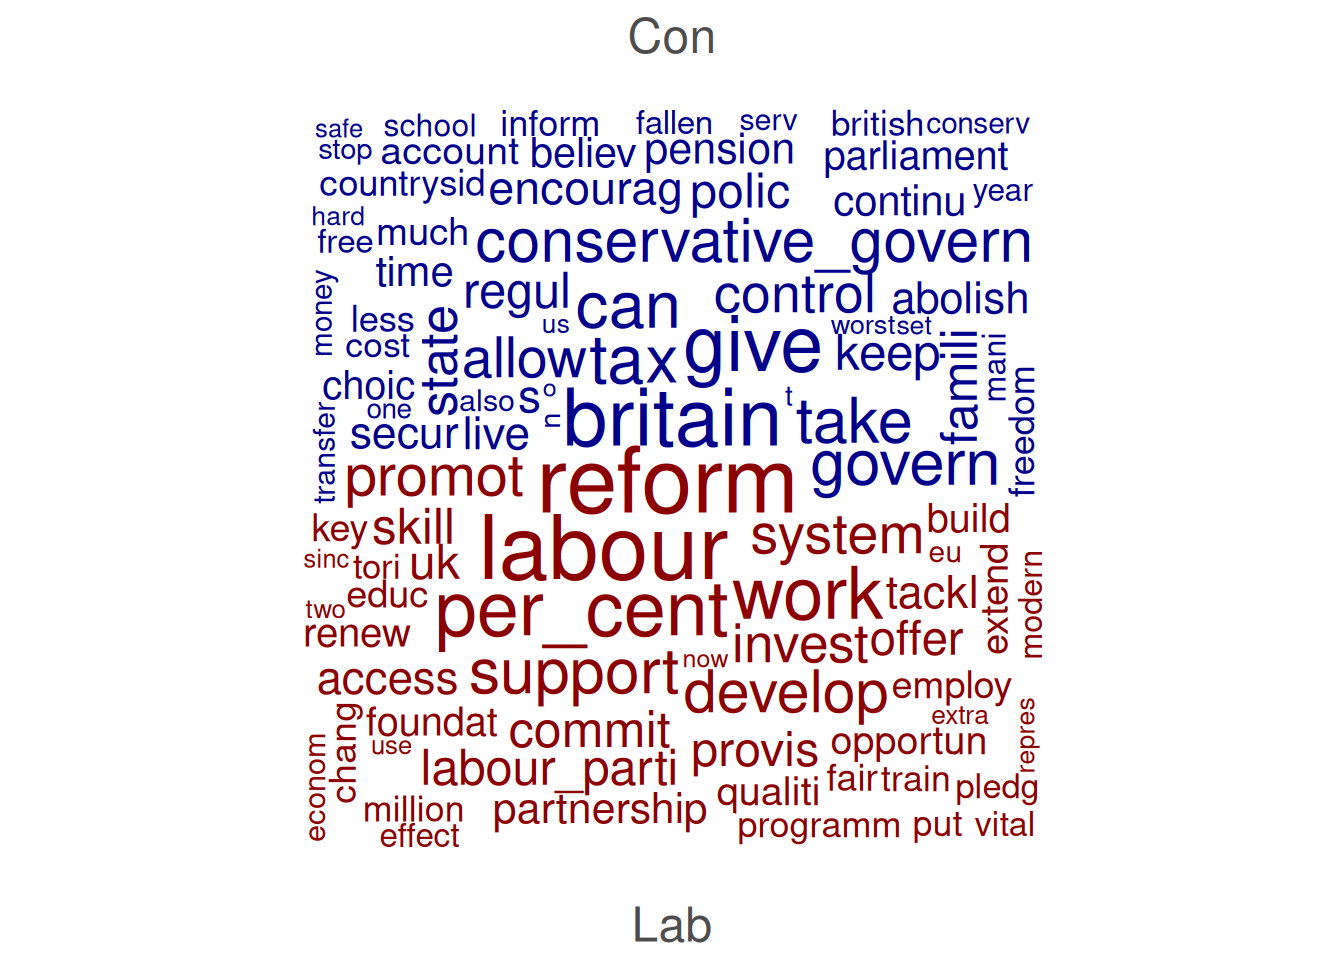
\includegraphics[keepaspectratio]{Introduction-to-Quantitative-Text-Analysis_files/figure-latex/wordcloud-compare-1.pdf}}

Another thing we can do is examine Keywords in Context (KWIC), which displays how specific words or phrases are used by showing them along with their surrounding words. This is useful for understanding the different senses of a word, identifying typical phrases it appears in, and exploring its usage across different documents or contexts. We perform KWIC analysis on the \texttt{tokens} object as the order of the words is still essential at this point:

\begin{Shaded}
\begin{Highlighting}[]
\CommentTok{\# pattern = \textquotesingle{}econom*\textquotesingle{}: The term to search for (using glob for wildcard}
\CommentTok{\# matching). This will find \textquotesingle{}econom\textquotesingle{}, \textquotesingle{}economi\textquotesingle{}, \textquotesingle{}economist\textquotesingle{}, etc., after}
\CommentTok{\# stemming.  valuetype = \textquotesingle{}glob\textquotesingle{}: Specifies that the pattern is a glob{-}style}
\CommentTok{\# wildcard pattern.  window = 3: Show 3 words before and 3 words after the}
\CommentTok{\# keyword.}

\NormalTok{kwic\_output }\OtherTok{\textless{}{-}} \FunctionTok{kwic}\NormalTok{(data\_tokens\_stemmed, }\AttributeTok{pattern =} \StringTok{"econom*"}\NormalTok{, }\AttributeTok{valuetype =} \StringTok{"glob"}\NormalTok{,}
    \AttributeTok{window =} \DecValTok{3}\NormalTok{)}
\FunctionTok{head}\NormalTok{(kwic\_output, }\DecValTok{10}\NormalTok{)}
\end{Highlighting}
\end{Shaded}

\begin{verbatim}
## Keyword-in-context with 10 matches.                                                                       
##   [UK_natl_1997_en_Con, 18]             europ becom success | economi |
##   [UK_natl_1997_en_Con, 67]        global free_market emerg | econom  |
##   [UK_natl_1997_en_Con, 89]            challeng turn around | econom  |
##  [UK_natl_1997_en_Con, 115]                lowest tax major | economi |
##  [UK_natl_1997_en_Con, 505]                 model fail just | econom  |
##  [UK_natl_1997_en_Con, 544]           opportun push forward | econom  |
##  [UK_natl_1997_en_Con, 580]             guis stakehold hard | econom  |
##  [UK_natl_1997_en_Con, 621] enterprise_centre_europ low tax | economi |
##  [UK_natl_1997_en_Con, 638]          public_spend choic two | econom  |
##  [UK_natl_1997_en_Con, 675]                 ensur grow less | economi |
##                               
##  countri brought knee         
##  power rise east              
##  fortun fewer_people_work work
##  europ mean continu           
##  triumph triumph human        
##  revolut began enter          
##  evid show great              
##  enterpris flourish state     
##  philosophi clear year        
##  whole economic_cycl time
\end{verbatim}

The \texttt{kwic()} function output includes the document name (\texttt{docname}), the position of the keyword (\texttt{from}, \texttt{to}), the surrounding context (\texttt{pre}, \texttt{post}), and the keyword itself (\texttt{keyword}).

\section{Text Statistics}\label{text-statistics}

Apart from graphics, we can also calculate a wide range of statistics about our texts, and the \texttt{quanteda.textstats} package offers a range of functions for this. We will use the pre-processed DFM (\texttt{data\_dfm\_trimmed}) and tokens (\texttt{data\_tokens\_stemmed}) for these calculations. We will go through the various options in turn.

\subsection{Summary}\label{summary}

\texttt{textstat\_summary()} provides basic summary statistics for each document in the corpus, such as the number of characters, tokens, types, sentences, and paragraphs. Note that this command works on the original corpus, and not on the cleaned DFM:

\begin{Shaded}
\begin{Highlighting}[]
\NormalTok{corpus\_summary }\OtherTok{\textless{}{-}} \FunctionTok{textstat\_summary}\NormalTok{(data\_corpus\_ukmanifestos)}
\FunctionTok{head}\NormalTok{(corpus\_summary)}
\end{Highlighting}
\end{Shaded}

\begin{verbatim}
##               document  chars sents tokens types puncts numbers symbols urls
## 1  UK_natl_1997_en_Con 131975  1188  23398  3174   2256     346       0    0
## 2  UK_natl_1997_en_Lab 111444   822  19372  3007   1787     114      15    0
## 3   UK_natl_1997_en_LD  90883   852  15988  2472   1766     104      38    0
## 4  UK_natl_1997_en_PCy 103411   765  17892  2969   1743      72       2    0
## 5   UK_natl_1997_en_SF  37998   254   6540  1629    620      55       8    0
## 6 UK_natl_1997_en_UKIP  72973   488  13103  2631   1195      61       8    0
##   tags emojis
## 1    0      0
## 2    0      0
## 3    0      0
## 4    0      0
## 5    0      0
## 6    0      0
\end{verbatim}

\subsection{Frequencies}\label{frequencies}

\texttt{textstat\_frequency()} provides detailed frequency counts for features in a DFM, including term frequency (total occurrences, like we already saw earlier) and document frequency (number of documents the term appears in). It can also group frequencies by document variables, allowing for comparison of term usage across different categories of documents.

\begin{Shaded}
\begin{Highlighting}[]
\NormalTok{feature\_frequencies }\OtherTok{\textless{}{-}} \FunctionTok{textstat\_frequency}\NormalTok{(data\_dfm\_trimmed)}
\FunctionTok{head}\NormalTok{(feature\_frequencies, }\DecValTok{10}\NormalTok{)}
\end{Highlighting}
\end{Shaded}

\begin{verbatim}
##    feature frequency rank docfreq group
## 1   govern       657    1      20   all
## 2     work       645    2      20   all
## 3     need       613    3      20   all
## 4  support       596    4      20   all
## 5  develop       589    5      19   all
## 6  increas       475    6      20   all
## 7  britain       465    7      16   all
## 8   provid       462    8      20   all
## 9    ensur       461    9      20   all
## 10  school       449   10      18   all
\end{verbatim}

\begin{Shaded}
\begin{Highlighting}[]
\NormalTok{party\_frequencies }\OtherTok{\textless{}{-}} \FunctionTok{textstat\_frequency}\NormalTok{(data\_dfm\_trimmed, }\AttributeTok{groups =}\NormalTok{ data\_dfm\_trimmed}\SpecialCharTok{@}\NormalTok{docvars}\SpecialCharTok{$}\NormalTok{Party)  }\CommentTok{\# Group by Party}
\FunctionTok{head}\NormalTok{(party\_frequencies, }\DecValTok{10}\NormalTok{)}
\end{Highlighting}
\end{Shaded}

\begin{verbatim}
##    feature frequency rank docfreq group
## 1  britain       141    1       3   Con
## 2   govern       124    2       3   Con
## 3   school        97    3       3   Con
## 4     give        87    4       3   Con
## 5     work        82    5       3   Con
## 6    peopl        79    6       3   Con
## 7      can        74    7       3   Con
## 8  continu        73    8       3   Con
## 9   labour        73    8       3   Con
## 10 pension        72   10       3   Con
\end{verbatim}

\subsection{Lexical diversity}\label{lexical-diversity}

Lexical diversity measures the variety of vocabulary in a text. \texttt{textstat\_lexdiv()} calculates various measures like the Type-Token Ratio (TTR), which is the number of types (unique tokens) divided by the total number of tokens. A higher TTR generally indicates greater lexical diversity. This function operates on a \texttt{tokens} object:

\begin{Shaded}
\begin{Highlighting}[]
\NormalTok{corpus\_lexdiv }\OtherTok{\textless{}{-}} \FunctionTok{textstat\_lexdiv}\NormalTok{(data\_tokens\_stemmed, }\AttributeTok{measure =} \StringTok{"TTR"}\NormalTok{)}
\NormalTok{corpus\_lexdiv}
\end{Highlighting}
\end{Shaded}

\begin{verbatim}
##                document       TTR
## 1   UK_natl_1997_en_Con 0.2733320
## 2   UK_natl_1997_en_Lab 0.3136331
## 3    UK_natl_1997_en_LD 0.3274956
## 4   UK_natl_1997_en_PCy 0.3124604
## 5    UK_natl_1997_en_SF 0.4374573
## 6  UK_natl_1997_en_UKIP 0.3505444
## 7   UK_natl_2001_en_Con 0.3433852
## 8   UK_natl_2001_en_Lab 0.2420945
## 9    UK_natl_2001_en_LD 0.2798416
## 10  UK_natl_2001_en_PCy 0.4446326
## 11   UK_natl_2001_en_SF 0.4259938
## 12  UK_natl_2001_en_SNP 0.3553472
## 13  UK_natl_2005_en_Con 0.4268849
## 14  UK_natl_2005_en_Lab 0.2891995
## 15   UK_natl_2005_en_LD 0.3209892
## 16  UK_natl_2005_en_PCy 0.4569697
## 17   UK_natl_2005_en_SF 0.2959165
## 18  UK_natl_2005_en_SNP 0.5817634
## 19 UK_natl_2005_en_UKIP 0.3882198
## 20  UK_regl_2003_en_PCy 0.2551293
\end{verbatim}

\subsection{Readability}\label{readability}

Readability statistics estimate the difficulty of understanding a text based on characteristics like sentence length and the number of syllables per word. \texttt{textstat\_readability()} calculates various standard scores (e.g., Flesch-Kincaid, Gunning Fog). This function works directly on a \texttt{corpus} object or a character vector:

\begin{Shaded}
\begin{Highlighting}[]
\NormalTok{corpus\_readability }\OtherTok{\textless{}{-}} \FunctionTok{textstat\_readability}\NormalTok{(data\_corpus\_ukmanifestos, }\AttributeTok{measure =} \StringTok{"Flesch.Kincaid"}\NormalTok{)}
\FunctionTok{head}\NormalTok{(corpus\_readability)}
\end{Highlighting}
\end{Shaded}

\begin{verbatim}
##               document Flesch.Kincaid
## 1  UK_natl_1997_en_Con       10.79018
## 2  UK_natl_1997_en_Lab       12.70561
## 3   UK_natl_1997_en_LD       11.10189
## 4  UK_natl_1997_en_PCy       13.48201
## 5   UK_natl_1997_en_SF       14.27023
## 6 UK_natl_1997_en_UKIP       13.82250
\end{verbatim}

\subsection{Similarity and Distance}\label{similarity-and-distance}

These functions calculate the similarity or distance between documents or features based on their representation in a DFM. They help quantify how alike or different texts or words are based on their shared vocabulary and term frequencies. Common measures include cosine similarity and Euclidean distance:

\begin{Shaded}
\begin{Highlighting}[]
\CommentTok{\# method = \textquotesingle{}cosine\textquotesingle{}: Specifies the cosine similarity measure.  margin =}
\CommentTok{\# \textquotesingle{}documents\textquotesingle{}: Calculate the similarity between documents (rows of the DFM).}

\NormalTok{corpus\_similarties }\OtherTok{\textless{}{-}} \FunctionTok{textstat\_simil}\NormalTok{(data\_dfm\_trimmed, }\AttributeTok{method =} \StringTok{"cosine"}\NormalTok{, }\AttributeTok{margin =} \StringTok{"documents"}\NormalTok{)}

\NormalTok{corpus\_similarties\_matrix }\OtherTok{\textless{}{-}} \FunctionTok{as.matrix}\NormalTok{(corpus\_similarties)}
\NormalTok{corpus\_similarties\_matrix[}\DecValTok{1}\SpecialCharTok{:}\DecValTok{5}\NormalTok{, }\DecValTok{1}\SpecialCharTok{:}\DecValTok{5}\NormalTok{]}
\end{Highlighting}
\end{Shaded}

\begin{verbatim}
##                     UK_natl_1997_en_Con UK_natl_1997_en_Lab UK_natl_1997_en_LD
## UK_natl_1997_en_Con           1.0000000           0.7569519          0.7502951
## UK_natl_1997_en_Lab           0.7569519           1.0000000          0.7528290
## UK_natl_1997_en_LD            0.7502951           0.7528290          1.0000000
## UK_natl_1997_en_PCy           0.6093673           0.6155356          0.6148482
## UK_natl_1997_en_SF            0.4817308           0.4968049          0.4681049
##                     UK_natl_1997_en_PCy UK_natl_1997_en_SF
## UK_natl_1997_en_Con           0.6093673          0.4817308
## UK_natl_1997_en_Lab           0.6155356          0.4968049
## UK_natl_1997_en_LD            0.6148482          0.4681049
## UK_natl_1997_en_PCy           1.0000000          0.4771206
## UK_natl_1997_en_SF            0.4771206          1.0000000
\end{verbatim}

\begin{Shaded}
\begin{Highlighting}[]
\CommentTok{\# method = \textquotesingle{}euclidean\textquotesingle{}: Specifies the Euclidean distance measure margin =}
\CommentTok{\# \textquotesingle{}documents\textquotesingle{}: Calculate the distance between documents}

\NormalTok{corpus\_distances }\OtherTok{\textless{}{-}} \FunctionTok{textstat\_dist}\NormalTok{(data\_dfm\_trimmed, }\AttributeTok{margin =} \StringTok{"documents"}\NormalTok{, }\AttributeTok{method =} \StringTok{"euclidean"}\NormalTok{)}

\CommentTok{\# Convert the distance object to a matrix for inspection of pairwise distances}

\NormalTok{corpus\_distances\_matrix }\OtherTok{\textless{}{-}} \FunctionTok{as.matrix}\NormalTok{(corpus\_distances)}
\NormalTok{corpus\_distances\_matrix[}\DecValTok{1}\SpecialCharTok{:}\DecValTok{5}\NormalTok{, }\DecValTok{1}\SpecialCharTok{:}\DecValTok{5}\NormalTok{]}
\end{Highlighting}
\end{Shaded}

\begin{verbatim}
##                     UK_natl_1997_en_Con UK_natl_1997_en_Lab UK_natl_1997_en_LD
## UK_natl_1997_en_Con              0.0000            230.1652           230.7423
## UK_natl_1997_en_Lab            230.1652              0.0000           197.8080
## UK_natl_1997_en_LD             230.7423            197.8080             0.0000
## UK_natl_1997_en_PCy            290.9605            262.1793           249.6117
## UK_natl_1997_en_SF             309.0372            257.2198           229.1244
##                     UK_natl_1997_en_PCy UK_natl_1997_en_SF
## UK_natl_1997_en_Con            290.9605           309.0372
## UK_natl_1997_en_Lab            262.1793           257.2198
## UK_natl_1997_en_LD             249.6117           229.1244
## UK_natl_1997_en_PCy              0.0000           266.7133
## UK_natl_1997_en_SF             266.7133             0.0000
\end{verbatim}

If we would want to, we can also visualise the distances between the documents in the form of a dendrogram, by clustering the distances object:

\begin{Shaded}
\begin{Highlighting}[]
\FunctionTok{plot}\NormalTok{(}\FunctionTok{hclust}\NormalTok{(}\FunctionTok{as.dist}\NormalTok{(corpus\_distances)))}
\end{Highlighting}
\end{Shaded}

\pandocbounded{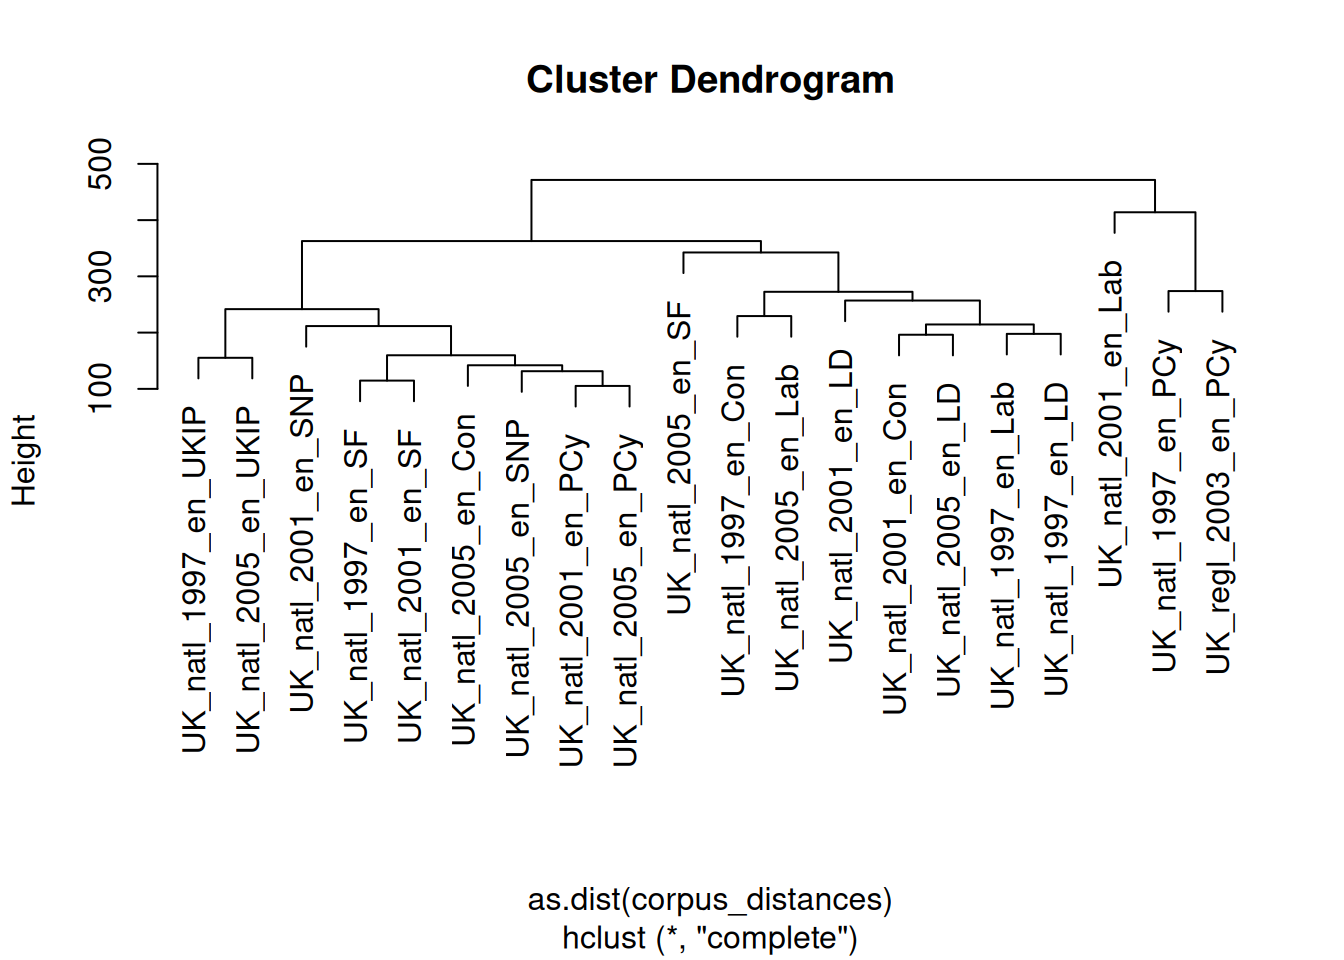
\includegraphics[keepaspectratio]{Introduction-to-Quantitative-Text-Analysis_files/figure-latex/dendrogram-1.pdf}}
The results here are quite interesting, for one in that while both the 1997 and 2003 Plaid Cymru documents are very similar, they are clustered together with the 2001 Labour Party document, which is quite far from its 1997 and 2005 counterparts.

\subsection{Keyness}\label{keyness}

Keyness statistics identify terms that are unusually frequent or infrequent in a target group of documents compared to a reference group. This is useful for identifying characteristic terms within a corpus subset and understanding what distinguishes one set of texts from another. A common measure is the log-likelihood ratio or chi-squared statistic:

\begin{Shaded}
\begin{Highlighting}[]
\CommentTok{\# Create a logical vector TRUE for documents from the Conservative party and}
\CommentTok{\# FALSE for others. This vector defines the \textquotesingle{}target\textquotesingle{} group.}

\NormalTok{data\_dfm\_trimmed}\SpecialCharTok{@}\NormalTok{docvars}\SpecialCharTok{$}\NormalTok{is\_conservative }\OtherTok{\textless{}{-}}\NormalTok{ data\_dfm\_trimmed}\SpecialCharTok{@}\NormalTok{docvars}\SpecialCharTok{$}\NormalTok{Party }\SpecialCharTok{==} \StringTok{"Con"}

\CommentTok{\# Compute keyness statistics comparing the Conservative manifestos (target) to}
\CommentTok{\# all other manifestos (reference) target =}
\CommentTok{\# data\_dfm\_trimmed@docvars$is\_conservative: Specifies the target group using}
\CommentTok{\# the logical vector}

\NormalTok{keyness\_conservative }\OtherTok{\textless{}{-}} \FunctionTok{textstat\_keyness}\NormalTok{(data\_dfm\_trimmed, }\AttributeTok{target =}\NormalTok{ data\_dfm\_trimmed}\SpecialCharTok{@}\NormalTok{docvars}\SpecialCharTok{$}\NormalTok{is\_conservative)}

\CommentTok{\# View the most distinctive terms for the Conservative party (highest keyness}
\CommentTok{\# scores) and the least distinctive terms (lowest keyness scores, which are}
\CommentTok{\# characteristic of the reference group)}

\FunctionTok{head}\NormalTok{(keyness\_conservative, }\DecValTok{20}\NormalTok{)}
\end{Highlighting}
\end{Shaded}

\begin{verbatim}
##                     feature      chi2            p n_target n_reference
## 1       conservative_govern 144.44686 0.000000e+00       38          14
## 2                   britain  94.85417 0.000000e+00      141         324
## 3  next_conservative_govern  93.74717 0.000000e+00       17           0
## 4                    famili  60.39675 7.771561e-15       69         137
## 5                     choic  54.78260 1.346701e-13       59         113
## 6                         n  52.41623 4.489742e-13       13           3
## 7                      keep  47.73544 4.877987e-12       47          85
## 8                   conserv  46.54836 8.938517e-12       61         131
## 9                    fallen  46.16172 1.088840e-11       19          14
## 10         time_common_sens  45.96519 1.203726e-11       10           1
## 11                    pound  45.15771 1.817879e-11       23          24
## 12                     give  44.16372 3.020273e-11       87         228
## 13                   contin  36.10094 1.873561e-09       10           3
## 14               foot_mouth  36.10094 1.873561e-09       10           3
## 15                lower_tax  35.07639 3.170212e-09        9           2
## 16                    widow  35.07639 3.170212e-09        9           2
## 17                  opt-out  34.50407 4.253600e-09        8           1
## 18                        w  34.50407 4.253600e-09        8           1
## 19               politician  30.71197 2.993130e-08       19          24
## 20                  continu  30.55484 3.245615e-08       73         207
\end{verbatim}

\begin{Shaded}
\begin{Highlighting}[]
\FunctionTok{tail}\NormalTok{(keyness\_conservative, }\DecValTok{20}\NormalTok{)}
\end{Highlighting}
\end{Shaded}

\begin{verbatim}
##               feature      chi2            p n_target n_reference
## 6238          poverti -12.58534 3.887848e-04        3         109
## 6239              snp -12.69011 3.675955e-04        0          75
## 6240       agricultur -13.31662 2.630645e-04        1          91
## 6241      all-ireland -13.87526 1.953533e-04        0          82
## 6242           access -13.90699 1.920823e-04       10         186
## 6243         strategi -14.88492 1.142728e-04        7         164
## 6244          resourc -15.33557 9.000581e-05       12         214
## 6245      environment -17.22185 3.325894e-05        4         148
## 6246             ukip -17.77023 2.492533e-05        0         105
## 6247           provis -18.75683 1.484903e-05        5         168
## 6248      plaid_cymru -18.78653 1.461959e-05        0         111
## 6249 liberal_democrat -19.72714 8.932357e-06        1         129
## 6250          develop -20.11047 7.309549e-06       47         542
## 6251               eu -20.27349 6.712432e-06       12         247
## 6252           promot -23.02328 1.600513e-06       18         321
## 6253            equal -23.45134 1.281138e-06        2         163
## 6254        sinn_féin -26.24228 3.011560e-07        0         155
## 6255         scotland -27.04384 1.988927e-07        3         196
## 6256               uk -28.18851 1.100557e-07       10         278
## 6257             wale -57.12540 4.085621e-14        2         362
\end{verbatim}

The output of \texttt{textstat\_keyness} includes the feature, the keyness score, and the \(p\)-value. Positive keyness scores indicate terms that are unusually frequent in the target group. In contrast, negative scores indicate terms unusually infrequent in the target group (and thus characteristic of the reference group). Here, these are words refering to ``britain'', the family (``famili''), and choice (``choic''). We can of course also visualise this:

\begin{Shaded}
\begin{Highlighting}[]
\FunctionTok{textplot\_keyness}\NormalTok{(keyness\_conservative)}
\end{Highlighting}
\end{Shaded}

\pandocbounded{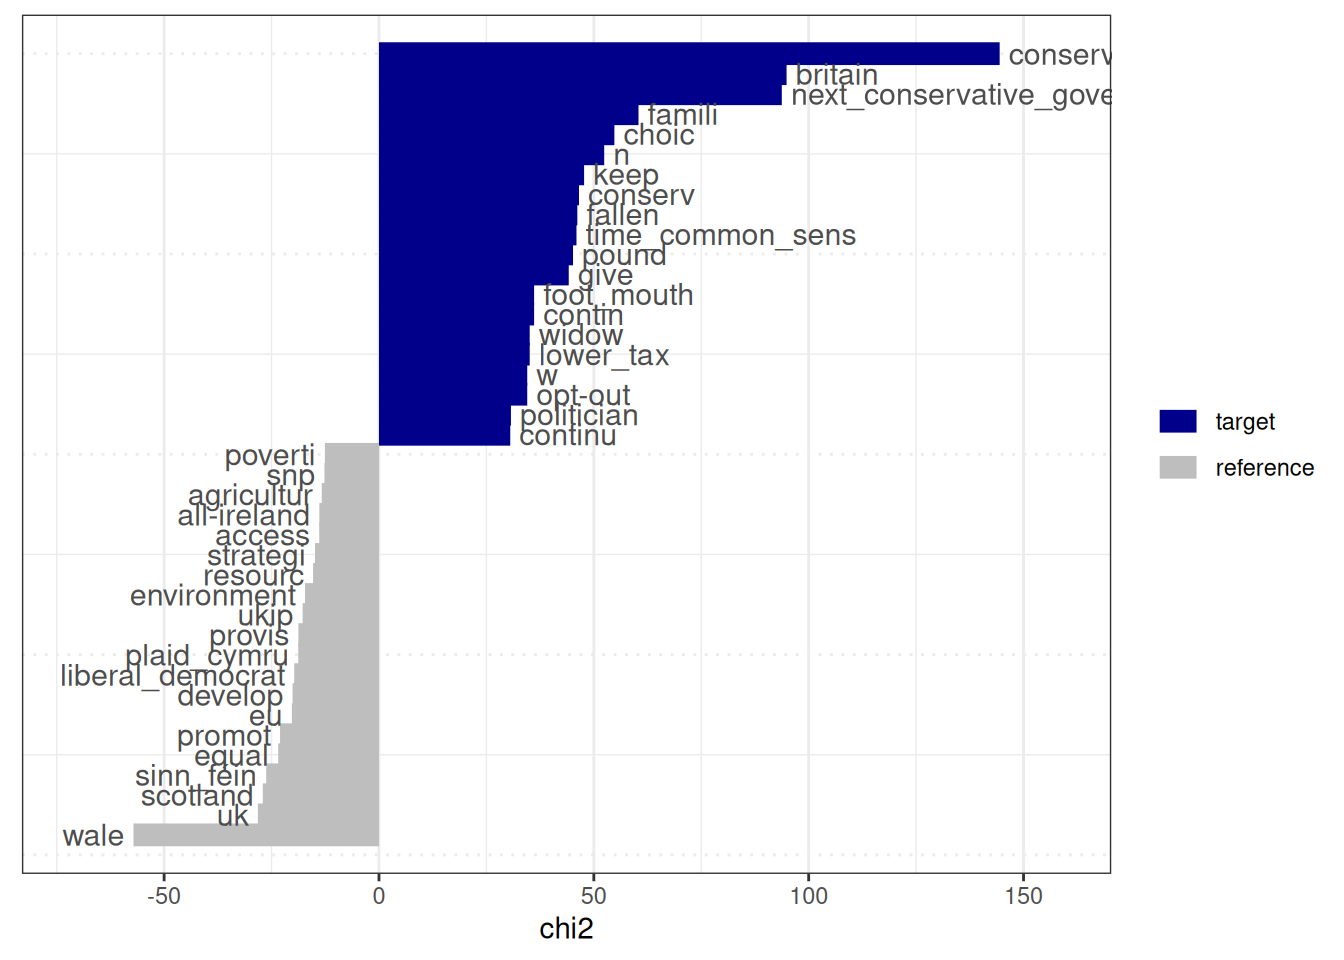
\includegraphics[keepaspectratio]{Introduction-to-Quantitative-Text-Analysis_files/figure-latex/textplot-keyness-1.pdf}}

\subsection{Entropy}\label{entropy}

Entropy measures the randomness or evenness of feature distributions. Here, we can use it to assess the diversity of terms within documents (document entropy) or the evenness of a term's distribution across the corpus (feature entropy). High document entropy means a document uses a wide variety of terms relatively evenly, while low entropy means a few terms dominate. High feature entropy means a term is spread relatively evenly across documents, while low entropy means it's concentrated in a few documents.

\begin{Shaded}
\begin{Highlighting}[]
\CommentTok{\# margin = \textquotesingle{}documents\textquotesingle{}: Calculate entropy for each document (rows of the DFM)}

\NormalTok{corpus\_entropy\_docs }\OtherTok{\textless{}{-}} \FunctionTok{textstat\_entropy}\NormalTok{(data\_dfm\_trimmed, }\AttributeTok{margin =} \StringTok{"documents"}\NormalTok{)}
\NormalTok{corpus\_entropy\_docs }\OtherTok{\textless{}{-}} \FunctionTok{as.data.frame}\NormalTok{(corpus\_entropy\_docs)}
\FunctionTok{head}\NormalTok{(corpus\_entropy\_docs)}
\end{Highlighting}
\end{Shaded}

\begin{verbatim}
##               document   entropy
## 1  UK_natl_1997_en_Con 10.332738
## 2  UK_natl_1997_en_Lab 10.383004
## 3   UK_natl_1997_en_LD 10.186036
## 4  UK_natl_1997_en_PCy 10.233130
## 5   UK_natl_1997_en_SF  9.619364
## 6 UK_natl_1997_en_UKIP 10.068977
\end{verbatim}

\begin{Shaded}
\begin{Highlighting}[]
\CommentTok{\# margin = \textquotesingle{}features\textquotesingle{}: Calculate entropy for each feature (columns of the DFM)}

\NormalTok{corpus\_entropy\_feats }\OtherTok{\textless{}{-}} \FunctionTok{textstat\_entropy}\NormalTok{(data\_dfm\_trimmed, }\AttributeTok{margin =} \StringTok{"features"}\NormalTok{)}
\NormalTok{corpus\_entropy\_feats }\OtherTok{\textless{}{-}} \FunctionTok{as.data.frame}\NormalTok{(corpus\_entropy\_feats)}
\NormalTok{corpus\_entropy\_feats }\OtherTok{\textless{}{-}}\NormalTok{ corpus\_entropy\_feats[}\FunctionTok{order}\NormalTok{(}\SpecialCharTok{{-}}\NormalTok{corpus\_entropy\_feats}\SpecialCharTok{$}\NormalTok{entropy),}
\NormalTok{    ]}
\FunctionTok{head}\NormalTok{(corpus\_entropy\_feats, }\DecValTok{10}\NormalTok{)}
\end{Highlighting}
\end{Shaded}

\begin{verbatim}
##      feature  entropy
## 4      elect 4.140895
## 16   economi 4.129012
## 86      mean 4.122883
## 380    parti 4.114558
## 1254    forc 4.110995
## 479   polici 4.110578
## 130  increas 4.107211
## 582     mani 4.101916
## 782  greater 4.101321
## 688  societi 4.097388
\end{verbatim}

\section{Exercises}\label{exercises}

\begin{enumerate}
\def\labelenumi{\arabic{enumi}.}
\item
  Using the UK Manifestos corpus (\texttt{data\_corpus\_ukmanifestos}), calculate each manifesto's readability scores (\texttt{textstat\_readability}), perhaps using multiple measures. Add these scores to the document variables and plot a chosen readability score against the \emph{Year} docvar. Is there a discernible trend in the readability of UK political manifestos over the selected period?
\item
  Calculate keyness statistics (\texttt{textstat\_keyness}) to compare Labour Party manifestos with all other parties in the filtered corpus. What are the 20 most important terms for the Labour Party? Create a visualisation of these terms using \texttt{textplot\_keyness}.
\item
  Using the cosine method (\texttt{margin\ =\ "features"}), explore the similarity of features (words) in the UK manifestos (\texttt{data\_dfm}). Can you identify pairs of words that tend to appear in similar contexts? (Hint: examine the similarity matrix for high values).
\item
  Calculate the entropy (\texttt{textstat\_entropy} ) for features in the UK Manifestos DFM. Identify features with very low entropy (close to 0) and examine the documents in which they are concentrated using the \texttt{kwic()} function or by examining the DFM directly. What might this tell you about those documents or the use of those specific terms?
\item
  Apply \texttt{textstat\_frequency} grouped by party to find the most frequent terms for the Conservative, Labour and Liberal Democrat parties. Create bar plots using the \texttt{ggplot2} package to visualise the frequencies of a few selected terms (e.g.~`econom', `social', `europ') across these three parties. Compare this to the grouped frequency plot above, and add more terms for comparison.
\end{enumerate}

\chapter{Dictionary Analysis}\label{dictionary-analysis}

One of the simplest forms of quantitative text analysis is dictionary analysis. The idea here is to count the presence of pre-defined categories of words or phrases within texts to classify documents or measure the extent to which documents relate to particular topics or sentiments. By relying on a fixed set of terms and associated categories, dictionary methods provide a transparent and computationally efficient approach to text analysis. Unlike statistical or machine learning methods that learn patterns from data, dictionary methods are \emph{non-statistical} and depend entirely on the quality and relevance of the dictionary used. A well-known application is measuring the tone of newspaper articles, speeches, children's writing, etc., using sentiment analysis dictionaries. These dictionaries categorise words as positive, negative or sometimes neutral, allowing a sentiment score to be calculated for a text. Another example is measuring the policy content of different documents, as illustrated by the Policy Agendas Project dictionary (\citeproc{ref-Albaugh2013a}{Albaugh et al., 2013}), which assigns words to various policy domains.

While straightforward, dictionary analysis has limitations. To begin with, it relies on the assumption that the meaning of a word is relatively stable across different contexts and documents. This can be a strong assumption, as the same word can have different meanings (polysemy), or its meaning can be negated or altered by surrounding words (e.g.~sarcasm). Besides, they also cannot identify concepts or themes not explicitly included in the dictionary. Despite these limitations, dictionary analysis remains a valuable tool, especially for exploratory analysis, when validated dictionaries are available or combined with other methods.

Here, we will conduct three analyses using dictionaries: the first is a standard content analysis approach using a political dictionary, and the other two focus on sentiment. For the former, we will use the same political party manifestos we used in the previous chapter, while for the latter, we will use film reviews and Twitter data.

\section{Classical Dictionary Analysis}\label{classical-dictionary-analysis}

We start with the classical version of dictionary analysis. As for these dictionaries, we can either create them ourselves or use an off-the-shelf version. As with the data, \texttt{quanteda} provides access to several off-the-shelf dictionaries relevant to the social sciences:

\begin{Shaded}
\begin{Highlighting}[]
\FunctionTok{library}\NormalTok{(quanteda.dictionaries)}
\end{Highlighting}
\end{Shaded}

We then apply one of these dictionaries to a document feature matrix (DFM), which is typically created from our corpus after appropriate pre-processing steps, such as tokenisation and lowercase and stopword removal, as we discussed in the previous chapter. As a dictionary, we will use the one created by Laver \& Garry (\citeproc{ref-Laver2000a}{2000}), which is designed to estimate political positions from political texts. We first load this dictionary into R and then run it on the DFM using the \texttt{dfm\_lookup} command. Here, you can use the DFM we created in the previous chapter, though, for this example, we make it from scratch (without any pre-processing):

\begin{Shaded}
\begin{Highlighting}[]
\FunctionTok{library}\NormalTok{(quanteda)}
\FunctionTok{library}\NormalTok{(quanteda.corpora)}
\FunctionTok{library}\NormalTok{(quanteda.dictionaries)}

\FunctionTok{data}\NormalTok{(data\_corpus\_ukmanifestos)}
\NormalTok{data\_corpus\_ukmanifestos}

\NormalTok{data\_tokens }\OtherTok{\textless{}{-}} \FunctionTok{tokens}\NormalTok{(data\_corpus\_ukmanifestos)}
\NormalTok{data\_dfm }\OtherTok{\textless{}{-}} \FunctionTok{dfm}\NormalTok{(data\_tokens)}
\end{Highlighting}
\end{Shaded}

First, let us have a look at the dictionary:

\begin{Shaded}
\begin{Highlighting}[]
\NormalTok{data\_dictionary\_LaverGarry  }\CommentTok{\# Display information about the dictionary object}
\end{Highlighting}
\end{Shaded}

\begin{verbatim}
## Dictionary object with 9 primary key entries and 2 nested levels.
## - [CULTURE]:
##   - people, war_in_iraq, civil_war
##   - [CULTURE-HIGH]:
##     - art, artistic, dance, galler*, museum*, music*, opera*, theatre*
##   - [CULTURE-POPULAR]:
##     - media
##   - [SPORT]:
##     - angler*
## - [ECONOMY]:
##   - [+STATE+]:
##     - accommodation, age, ambulance, assist, benefit, care, carer*, child*, class, classes, clinics, collective*, contribution*, cooperative*, co-operative*, deprivation, disabilities, disadvantaged, educat*, elderly [ ... and 30 more ]
##   - [=STATE=]:
##     - accountant, accounting, accounts, advert*, airline*, airport*, audit*, bank*, bargaining, breadwinner*, budget*, buy*, cartel*, cash*, charge*, commerce*, compensat*, consum*, cost*, credit* [ ... and 51 more ]
##   - [-STATE-]:
##     - assets, autonomy, barrier*, bid, bidders, bidding, burden*, charit*, choice*, compet*, confidence, confiscatory, constrain*, contracting*, contractor*, controlled, controlling, controls, corporate, corporation* [ ... and 42 more ]
## - [ENVIRONMENT]:
##   - [CON ENVIRONMENT]:
##     - produc*
##   - [PRO ENVIRONMENT]:
##     - car, catalytic, chemical*, chimney*, clean*, congestion, cyclist*, deplet*, ecolog*, emission*, energy-saving, environment*, fur, green, habitat*, hedgerow*, husbanded, litter*, opencast, open-cast* [ ... and 8 more ]
## - [GROUPS]:
##   - [ETHNIC]:
##     - asian*, buddhist*, ethnic*, race, raci*
##   - [WOMEN]:
##     - girls, woman, women
## - [INSTITUTIONS]:
##   - [CONSERVATIVE]:
##     - authority, continu*, disrupt*, inspect*, jurisdiction*, legitimate, manag*, moratorium, rul*, strike*, whitehall
##   - [NEUTRAL]:
##     - administr*, advis*, agenc*, amalgamat*, appoint*, assembly, chair*, commission*, committee*, constituen*, council*, department*, directorate*, executive*, headquarters, legislat*, mechanism*, minister*, office, offices [ ... and 18 more ]
##   - [RADICAL]:
##     - abolition, accountable, answerable, consult*, corrupt*, democratic*, elect*, implement*, modern*, monitor*, rebuild*, reexamine*, reform*, re-organi*, repeal*, replace*, representat*, scandal*, scrap, scrap* [ ... and 3 more ]
## - [LAW_AND_ORDER]:
##   - [LAW-CONSERVATIVE]:
##     - assaults, bail, burglar*, constab*, convict*, court, courts, custod*, dealing, delinquen*, deter, deter*, disorder, drug*, fine, fines, firmness, force*, fraud*, guard* [ ... and 32 more ]
##   - [LAW-LIBERAL]:
##     - harassment, non-custodial
## [ reached max_nkey ... 3 more keys ]
\end{verbatim}

Then, we apply it to the DFM:

\begin{Shaded}
\begin{Highlighting}[]
\NormalTok{dictionary\_results }\OtherTok{\textless{}{-}} \FunctionTok{dfm\_lookup}\NormalTok{(data\_dfm, data\_dictionary\_LaverGarry)}
\NormalTok{dictionary\_results}
\end{Highlighting}
\end{Shaded}

\begin{verbatim}
## Document-feature matrix of: 101 documents, 20 features (17.23% sparse) and 6 docvars.
##                      features
## docs                  CULTURE.CULTURE-HIGH CULTURE.CULTURE-POPULAR
##   UK_natl_1945_en_Con                    5                       0
##   UK_natl_1945_en_Lab                    3                       0
##   UK_natl_1945_en_Lib                    5                       0
##   UK_natl_1950_en_Con                    2                       0
##   UK_natl_1950_en_Lab                    1                       0
##   UK_natl_1950_en_Lib                    2                       0
##                      features
## docs                  CULTURE.SPORT CULTURE ECONOMY.+STATE+ ECONOMY.=STATE=
##   UK_natl_1945_en_Con             0      14              66             119
##   UK_natl_1945_en_Lab             0      24              61             150
##   UK_natl_1945_en_Lib             0       8              43             106
##   UK_natl_1950_en_Con             0      11              74             217
##   UK_natl_1950_en_Lab             0      23              56             146
##   UK_natl_1950_en_Lib             0       3              44              99
##                      features
## docs                  ECONOMY.-STATE- ENVIRONMENT.CON ENVIRONMENT
##   UK_natl_1945_en_Con              61                          12
##   UK_natl_1945_en_Lab              67                          18
##   UK_natl_1945_en_Lib              42                           6
##   UK_natl_1950_en_Con              86                          22
##   UK_natl_1950_en_Lab              77                          15
##   UK_natl_1950_en_Lib              48                          11
##                      features
## docs                  ENVIRONMENT.PRO ENVIRONMENT GROUPS.ETHNIC
##   UK_natl_1945_en_Con                           0             0
##   UK_natl_1945_en_Lab                           1             0
##   UK_natl_1945_en_Lib                           4             0
##   UK_natl_1950_en_Con                           3             0
##   UK_natl_1950_en_Lab                           2             0
##   UK_natl_1950_en_Lib                           0             0
## [ reached max_ndoc ... 95 more documents, reached max_nfeat ... 10 more features ]
\end{verbatim}

Here, we see that -- for example -- the 1945 Conservative Party manifesto -- contained 5 words related to High Culture while it contained none for Popular Culture. Overall, the \texttt{dfm\_lookup()} function takes a DFM and a dictionary object as input and returns a new DFM where the features are the categories defined in the dictionary and the values are the aggregated counts of terms belonging to each category within each document.

We can create our own dictionaries that better suit our research question or context. For this, we draw on our theoretical framework to develop different categories and their associated words. Another approach is using reference texts or expert knowledge to identify relevant category terms. We can also combine different dictionaries, as illustrated by Young \& Soroka (\citeproc{ref-Young2012a}{2012}), or integrate keywords from manual coding schemes (\citeproc{ref-Lind2019a}{Lind et al., 2019}). In addition, we can use techniques involving expert or crowd-coding assessments to refine dictionaries or determine the words that best fit different categories (\citeproc{ref-Haselmayer2017a}{Haselmayer \& Jenny, 2017}).

If we want to create our dictionary in \texttt{quanteda}, we use the \texttt{dictionary()} command. To do this, we specify the words in a named list. This list contains keys (the names of the categories) and the values, which are character vectors containing the words or phrases belonging to each category. We can use wildcard characters (such as \texttt{*} for glob matching) to include word variations. We then convert this list into a dictionary object. Here, we choose some words that we think will allow us to identify different political stances or issues:

\begin{Shaded}
\begin{Highlighting}[]
\NormalTok{dic\_list }\OtherTok{\textless{}{-}} \FunctionTok{list}\NormalTok{(}
    \AttributeTok{economy =} \FunctionTok{c}\NormalTok{(}\StringTok{"tax*"}\NormalTok{, }\StringTok{"invest*"}\NormalTok{, }\StringTok{"trade"}\NormalTok{, }\StringTok{"fiscal policy"}\NormalTok{), }\CommentTok{\# Include a multi{-}word phrase}
    \AttributeTok{war =} \FunctionTok{c}\NormalTok{(}\StringTok{"army"}\NormalTok{, }\StringTok{"troops"}\NormalTok{, }\StringTok{"fight*"}\NormalTok{, }\StringTok{"military"}\NormalTok{),}
    \AttributeTok{diplomacy =} \FunctionTok{c}\NormalTok{(}\StringTok{"nato"}\NormalTok{, }\StringTok{"un"}\NormalTok{, }\StringTok{"international relations"}\NormalTok{), }
    \AttributeTok{government =} \FunctionTok{c}\NormalTok{(}\StringTok{"london"}\NormalTok{, }\StringTok{"commons"}\NormalTok{, }\StringTok{"downing street"}\NormalTok{, }\StringTok{"westminster"}\NormalTok{)}
\NormalTok{)}

\CommentTok{\# tolower = TRUE is often recommended unless you have a specific reason not to lowercase}

\NormalTok{dic\_created }\OtherTok{\textless{}{-}} \FunctionTok{dictionary}\NormalTok{(dic\_list, }\AttributeTok{tolower =} \ConstantTok{TRUE}\NormalTok{)}
\NormalTok{dic\_created}
\end{Highlighting}
\end{Shaded}

\begin{verbatim}
## Dictionary object with 4 key entries.
## - [economy]:
##   - tax*, invest*, trade, fiscal policy
## - [war]:
##   - army, troops, fight*, military
## - [diplomacy]:
##   - nato, un, international relations
## - [government]:
##   - london, commons, downing street, westminster
\end{verbatim}

If you compare the structure of \texttt{dic\_list} and the resulting \texttt{dic\_created} object with that of \texttt{data\_dictionary\_LaverGarry}, you will see that they have a similar structure, defining categories and associated terms. To then apply our created dictionary to the dfm, we use the same `dfm\_lookup' command:

\begin{Shaded}
\begin{Highlighting}[]
\CommentTok{\# Ensure the dfm used here is preprocessed with tolower = TRUE if the}
\CommentTok{\# dictionary is lowercased}

\NormalTok{dictionary\_dfm }\OtherTok{\textless{}{-}} \FunctionTok{dfm\_lookup}\NormalTok{(data\_dfm, dic\_created)}
\NormalTok{dictionary\_dfm}
\end{Highlighting}
\end{Shaded}

\begin{verbatim}
## Document-feature matrix of: 101 documents, 4 features (16.58% sparse) and 6 docvars.
##                      features
## docs                  economy war diplomacy government
##   UK_natl_1945_en_Con      24   4         0          0
##   UK_natl_1945_en_Lab      13   5         0          0
##   UK_natl_1945_en_Lib      12   5         0          1
##   UK_natl_1950_en_Con      31   4         0          4
##   UK_natl_1950_en_Lab      11   1         0          0
##   UK_natl_1950_en_Lib      20   3         0          1
## [ reached max_ndoc ... 95 more documents ]
\end{verbatim}

Note that \texttt{dfm\_lookup()} matches individual features (words) in the dfm to the dictionary entries. This means that it will correctly match \texttt{"tax"}, \texttt{"taxes"}, \texttt{"taxation"} to the ``economy'' category if \texttt{"tax*"} is in the dictionary. However, if our dictionary contains multi-word expressions (like \texttt{"fiscal\ policy"} or \texttt{"international\ relations"} in our example \texttt{dic\_list}), \texttt{dfm\_lookup()} will not find them because the dfm loses word order information.

To correctly count multi-word expressions defined in a dictionary, we should apply the dictionary \emph{before} creating the dfm directly to the \texttt{tokens\textquotesingle{}\ object\ using\ the}tokens\_lookup()\texttt{function.\ tokens\_lookup()} preserves the order of the tokens and can therefore match multi-word phrases. The output of \texttt{tokens\_lookup()} is a \texttt{tokens} object where the original tokens are replaced by their dictionary categories. We can then convert the resulting token object into a dfm if necessary:

\begin{Shaded}
\begin{Highlighting}[]
\CommentTok{\# Use tokens\_lookup to handle multi{-}word expressions}

\NormalTok{dictionary\_tokens }\OtherTok{\textless{}{-}} \FunctionTok{tokens\_lookup}\NormalTok{(data\_tokens, dic\_created, }\AttributeTok{exclusive =} \ConstantTok{FALSE}\NormalTok{)  }\CommentTok{\# exclusive=FALSE allows tokens to match multiple categories if applicable}

\NormalTok{dictionary\_tokens\_dfm }\OtherTok{\textless{}{-}} \FunctionTok{dfm}\NormalTok{(dictionary\_tokens)}
\end{Highlighting}
\end{Shaded}

Comparing \texttt{dictionary\_created\_dfm} and \texttt{dictionary\_created\_dfm\_from\_tokens} shows that the latter correctly identifies and counts the multi-word expressions defined in \texttt{dic\_created}. Using \texttt{tokens\_lookup()} with \texttt{exclusive\ =\ FALSE} means a token can be assigned to multiple categories if it matches entries in more than one. Setting \texttt{exclusive\ =\ TRUE} would assign a token to only one category (the first found match). Furthermore, while we can view the resulting dfm by calling it in the console or viewing it in the environment, we can also convert this dfm into a regular data frame for easier manipulation and visualisation. For this, we can use the \texttt{convert} command included in \texttt{quanteda}:

\begin{Shaded}
\begin{Highlighting}[]
\NormalTok{dictionary\_df }\OtherTok{\textless{}{-}} \FunctionTok{convert}\NormalTok{(dictionary\_tokens\_dfm, }\AttributeTok{to =} \StringTok{"data.frame"}\NormalTok{)}
\end{Highlighting}
\end{Shaded}

You can then use this data frame to normalise these raw counts and compare dictionary results across documents of different lengths by dividing the category counts by either the total number of tokens or the total number of dictionary words in each document.

\section{Sentiment Analysis}\label{sentiment-analysis}

The logic of dictionaries extends beyond simple words, as we saw above; we can also use them to provide measures related to scaling, such as the degree of positive or negative sentiment and look at whether a text expresses happiness, anger, positivity, negativity, etc. This can be particularly useful for analysing subjective content such as movie reviews, which we will look at in the first example.

\subsection{Movie Reviews}\label{movie-reviews}

Movie reviews often describe a film alongside an explicit opinion or rating. Here, we will use a sample from the Large Movie Review Dataset (\texttt{data\_corpus\_LMRD}), which contains reviews labelled as either positive or negative and which sometimes have ratings associated with them. As the dataset is large, we will work with a smaller sample of 30 reviews for demonstration purposes. We will sample the corpus using the \texttt{corpus\_sample()} function and then preprocess it by tokenising, lowercasing, and removing stop words before creating a document feature matrix (DFM):

\begin{Shaded}
\begin{Highlighting}[]
\FunctionTok{library}\NormalTok{(quanteda.classifiers)}
\FunctionTok{library}\NormalTok{(quanteda)}

\CommentTok{\# Load the large movie review dataset and sample 30 reviews}
\FunctionTok{data}\NormalTok{(data\_corpus\_LMRD)}
\FunctionTok{set.seed}\NormalTok{(}\DecValTok{42}\NormalTok{)  }\CommentTok{\# Set seed for reproducibility}
\NormalTok{reviews }\OtherTok{\textless{}{-}} \FunctionTok{corpus\_sample}\NormalTok{(data\_corpus\_LMRD, }\DecValTok{30}\NormalTok{)}

\NormalTok{reviews\_tokens }\OtherTok{\textless{}{-}} \FunctionTok{tokens}\NormalTok{(reviews, }\AttributeTok{remove\_punct =} \ConstantTok{TRUE}\NormalTok{, }\AttributeTok{remove\_symbols =} \ConstantTok{TRUE}\NormalTok{, }\AttributeTok{remove\_numbers =} \ConstantTok{TRUE}\NormalTok{,}
    \AttributeTok{remove\_url =} \ConstantTok{TRUE}\NormalTok{)}
\NormalTok{reviews\_tokens }\OtherTok{\textless{}{-}} \FunctionTok{tokens\_tolower}\NormalTok{(reviews\_tokens)}
\NormalTok{reviews\_tokens }\OtherTok{\textless{}{-}} \FunctionTok{tokens\_select}\NormalTok{(reviews\_tokens, }\FunctionTok{stopwords}\NormalTok{(}\StringTok{"english"}\NormalTok{), }\AttributeTok{selection =} \StringTok{"remove"}\NormalTok{)}
\NormalTok{reviews\_dfm }\OtherTok{\textless{}{-}} \FunctionTok{dfm}\NormalTok{(reviews\_tokens)}
\end{Highlighting}
\end{Shaded}

The next step is to load a sentiment analysis dictionary and apply it to our film review dfm. Here, we will use the Lexicoder Sentiment Dictionary (LSD2015), which is included in \texttt{quanteda.dictionaries}. This dictionary categorises words as positive or negative. We use the dictionary with \texttt{dfm\_lookup()}:

\begin{Shaded}
\begin{Highlighting}[]
\FunctionTok{library}\NormalTok{(quanteda.dictionaries)}
\NormalTok{data\_dictionary\_LSD2015}

\NormalTok{results\_dfm }\OtherTok{\textless{}{-}} \FunctionTok{dfm\_lookup}\NormalTok{(reviews\_dfm, data\_dictionary\_LSD2015)}
\NormalTok{results\_dfm}
\end{Highlighting}
\end{Shaded}

The resulting \texttt{results\_dfm} has features corresponding to the categories in the LSD2015 dictionary (e.g., ``positive'' and ``negative''), and the values are the number of words in each category found in each film review. The next step then is to convert the results into a data frame for easier analysis and display:

\begin{Shaded}
\begin{Highlighting}[]
\NormalTok{sentiment }\OtherTok{\textless{}{-}} \FunctionTok{convert}\NormalTok{(results\_dfm, }\AttributeTok{to =} \StringTok{"data.frame"}\NormalTok{)}
\FunctionTok{head}\NormalTok{(sentiment)}
\end{Highlighting}
\end{Shaded}

\begin{verbatim}
##                 doc_id negative positive neg_positive neg_negative
## 1 train/neg/6869_1.txt       19       31            0            0
## 2  test/neg/6694_1.txt        8        7            0            0
## 3 train/pos/6588_9.txt        8       12            0            0
## 4 train/pos/7415_8.txt        5       13            0            0
## 5  test/pos/2566_9.txt        8        9            0            0
## 6  test/neg/5680_2.txt       31       19            0            0
\end{verbatim}

Often, movie reviews have an external rating (often in the form of stars or a positive/negative label). In that case, we can see if the dictionary-based sentiment is related to that rating. As the \texttt{data\_corpus\_LMRD} sample contains these ratings as document variables (docvars), we can extract this easily:

\begin{Shaded}
\begin{Highlighting}[]
\NormalTok{star\_data }\OtherTok{\textless{}{-}} \FunctionTok{docvars}\NormalTok{(reviews, }\AttributeTok{field =} \StringTok{"rating"}\NormalTok{)}

\CommentTok{\# Combine the rating with the dictionary sentiment scores}

\NormalTok{stargraph }\OtherTok{\textless{}{-}} \FunctionTok{as.data.frame}\NormalTok{(}\FunctionTok{cbind}\NormalTok{(star\_data, sentiment}\SpecialCharTok{$}\NormalTok{negative, sentiment}\SpecialCharTok{$}\NormalTok{positive))}
\FunctionTok{names}\NormalTok{(stargraph) }\OtherTok{\textless{}{-}} \FunctionTok{c}\NormalTok{(}\StringTok{"stars"}\NormalTok{, }\StringTok{"negative"}\NormalTok{, }\StringTok{"positive"}\NormalTok{)}
\FunctionTok{head}\NormalTok{(stargraph)}
\end{Highlighting}
\end{Shaded}

\begin{verbatim}
##   stars negative positive
## 1     1       19       31
## 2     1        8        7
## 3     9        8       12
## 4     8        5       13
## 5     9        8        9
## 6     2       31       19
\end{verbatim}

Now, we can combine the positive and negative counts into a single sentiment score to compare dictionary-based sentiment with star ratings. For this, we take the ratio of positive words to the total number of sentiment words (\(positive / (positive + negative)\)) to avoid division by zero if there are no positive or negative words:

\begin{Shaded}
\begin{Highlighting}[]
\NormalTok{sentiment\_ratio }\OtherTok{\textless{}{-}}\NormalTok{ stargraph}\SpecialCharTok{$}\NormalTok{positive}\SpecialCharTok{/}\NormalTok{(stargraph}\SpecialCharTok{$}\NormalTok{positive }\SpecialCharTok{+}\NormalTok{ stargraph}\SpecialCharTok{$}\NormalTok{negative)}

\NormalTok{stargraph }\OtherTok{\textless{}{-}} \FunctionTok{cbind}\NormalTok{(stargraph, sentiment\_ratio)}
\FunctionTok{head}\NormalTok{(stargraph)}
\end{Highlighting}
\end{Shaded}

\begin{verbatim}
##   stars negative positive sentiment_ratio
## 1     1       19       31       0.6200000
## 2     1        8        7       0.4666667
## 3     9        8       12       0.6000000
## 4     8        5       13       0.7222222
## 5     9        8        9       0.5294118
## 6     2       31       19       0.3800000
\end{verbatim}

Using \texttt{ggplot2}, we can plot the star ratings against these scaled sentiment measures to assess the relationship visually:

\begin{Shaded}
\begin{Highlighting}[]
\FunctionTok{library}\NormalTok{(ggplot2)}

\FunctionTok{ggplot}\NormalTok{(stargraph, }\FunctionTok{aes}\NormalTok{(}\AttributeTok{x =}\NormalTok{ sentiment\_ratio, }\AttributeTok{y =}\NormalTok{ stars)) }\SpecialCharTok{+} \FunctionTok{geom\_point}\NormalTok{(}\AttributeTok{shape =} \DecValTok{1}\NormalTok{) }\SpecialCharTok{+}
    \FunctionTok{geom\_smooth}\NormalTok{(}\AttributeTok{method =}\NormalTok{ lm, }\AttributeTok{se =} \ConstantTok{FALSE}\NormalTok{, }\AttributeTok{color =} \StringTok{"black"}\NormalTok{) }\SpecialCharTok{+} \FunctionTok{scale\_y\_continuous}\NormalTok{(}\AttributeTok{name =} \StringTok{"Star Rating"}\NormalTok{,}
    \AttributeTok{limits =} \FunctionTok{c}\NormalTok{(}\DecValTok{0}\NormalTok{, }\FloatTok{10.5}\NormalTok{), }\AttributeTok{expand =} \FunctionTok{c}\NormalTok{(}\DecValTok{0}\NormalTok{, }\DecValTok{0}\NormalTok{)) }\SpecialCharTok{+} \FunctionTok{scale\_x\_continuous}\NormalTok{(}\AttributeTok{name =} \StringTok{"Ratio of Positive to Total Sentiment Words"}\NormalTok{,}
    \AttributeTok{limits =} \FunctionTok{c}\NormalTok{(}\DecValTok{0}\NormalTok{, }\DecValTok{1}\NormalTok{), }\AttributeTok{expand =} \FunctionTok{c}\NormalTok{(}\DecValTok{0}\NormalTok{, }\DecValTok{0}\NormalTok{)) }\SpecialCharTok{+} \FunctionTok{ggtitle}\NormalTok{(}\StringTok{"Sentiment Ratio vs. Star Rating"}\NormalTok{) }\SpecialCharTok{+}
    \FunctionTok{theme\_classic}\NormalTok{()}
\end{Highlighting}
\end{Shaded}

\begin{verbatim}
## `geom_smooth()` using formula = 'y ~ x'
\end{verbatim}

\pandocbounded{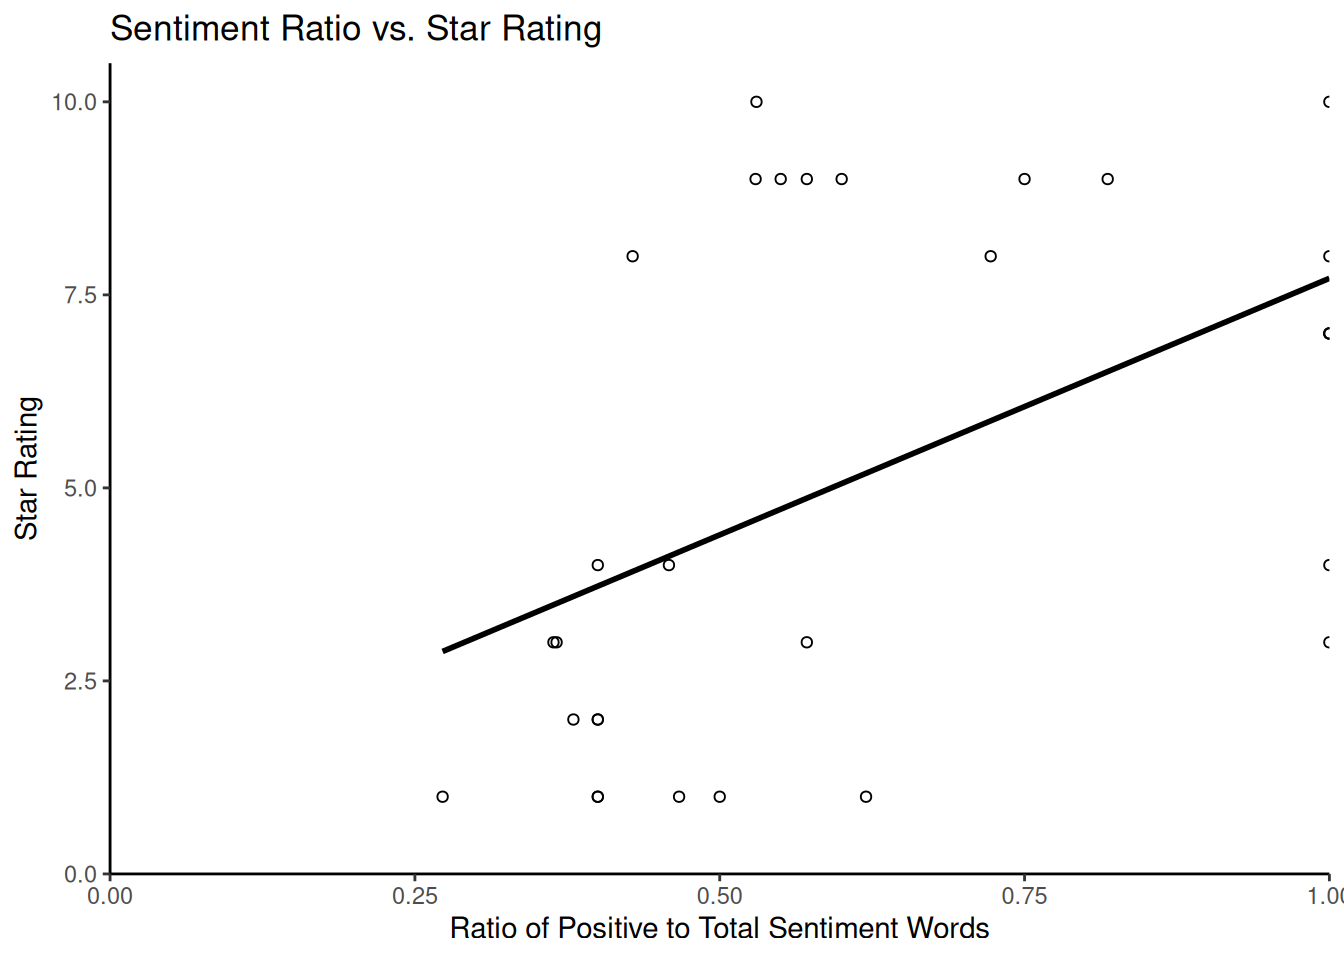
\includegraphics[keepaspectratio]{Introduction-to-Quantitative-Text-Analysis_files/figure-latex/ggplot-moviereviews-stars-1.pdf}}

Finally, we consider how to estimate the uncertainty around our dictionary-based sentiment scores, particularly the percentages of positive or negative words. For this, we use bootstrapping, a statistical technique that calculates the sampling variability of a statistic by resampling the observed data. In the context of text analysis and dictionary methods, bootstrapping can help us quantify the uncertainty in the estimated proportion of words falling into particular dictionary categories within each document. This is particularly useful for understanding the reliability of scores for shorter documents with limited word counts.

The following code demonstrates a bootstrapping approach to estimating confidence intervals for the percentage of positive and negative words in each review. This method involves resampling the word counts within each document based on a multinomial distribution derived from the observed counts. While the code may appear complex, it essentially simulates drawing new sets of words for each document many times based on the proportions of positive and negative words found initially. The core logic is that the \texttt{apply} function with \texttt{rmultinom} simulates drawing new counts for the negative and positive categories based on their observed proportions and the total number of sentiment words in each document. We repeat this process \texttt{nrepl} several times to obtain a distribution of possible percentages for each document under resampling. The standard deviation of these simulated percentages estimates the standard error, which is then used to calculate confidence intervals.

\begin{Shaded}
\begin{Highlighting}[]
\FunctionTok{library}\NormalTok{(ggplot2)  }\CommentTok{\# For plotting}
\FunctionTok{library}\NormalTok{(dplyr)}

\CommentTok{\# Prepare data for bootstrapping: include doc\_id and sentiment counts}

\NormalTok{reviews\_bootstrap\_data }\OtherTok{\textless{}{-}}\NormalTok{ sentiment[, }\FunctionTok{c}\NormalTok{(}\StringTok{"doc\_id"}\NormalTok{, }\StringTok{"negative"}\NormalTok{, }\StringTok{"positive"}\NormalTok{)]}

\CommentTok{\# Remove rows with zero total sentiment words to avoid division by zero issues}
\CommentTok{\# later}
\NormalTok{reviews\_bootstrap\_data }\OtherTok{\textless{}{-}}\NormalTok{ reviews\_bootstrap\_data }\SpecialCharTok{\%\textgreater{}\%}
    \FunctionTok{filter}\NormalTok{(negative }\SpecialCharTok{+}\NormalTok{ positive }\SpecialCharTok{\textgreater{}} \DecValTok{0}\NormalTok{)}

\CommentTok{\# Get the number of documents remaining}
\NormalTok{nman }\OtherTok{\textless{}{-}} \FunctionTok{nrow}\NormalTok{(reviews\_bootstrap\_data)}

\CommentTok{\# Set parameters for bootstrapping}
\NormalTok{nrepl }\OtherTok{\textless{}{-}} \DecValTok{1000}  \CommentTok{\# Number of bootstrap replications}

\CommentTok{\# {-}{-}{-} Perform Bootstrapping {-}{-}{-} We will store the results of each bootstrap}
\CommentTok{\# replication in a list}
\NormalTok{bootstrap\_reps }\OtherTok{\textless{}{-}} \FunctionTok{vector}\NormalTok{(}\StringTok{"list"}\NormalTok{, nrepl)}

\ControlFlowTok{for}\NormalTok{ (i }\ControlFlowTok{in} \DecValTok{1}\SpecialCharTok{:}\NormalTok{nrepl) \{}
    \CommentTok{\# For each document, simulate drawing word counts from a multinomial}
    \CommentTok{\# distribution The number of trials is the total sentiment words in the}
    \CommentTok{\# document The probabilities are the observed proportions of}
    \CommentTok{\# negative/positive words}
\NormalTok{    boot\_counts }\OtherTok{\textless{}{-}} \FunctionTok{t}\NormalTok{(}\FunctionTok{apply}\NormalTok{(reviews\_bootstrap\_data[, }\FunctionTok{c}\NormalTok{(}\StringTok{"negative"}\NormalTok{, }\StringTok{"positive"}\NormalTok{)], }\DecValTok{1}\NormalTok{,}
        \ControlFlowTok{function}\NormalTok{(x) \{}
\NormalTok{            total\_words }\OtherTok{\textless{}{-}} \FunctionTok{sum}\NormalTok{(x)}
            \CommentTok{\# Use rmultinom to draw new counts}
            \FunctionTok{rmultinom}\NormalTok{(}\DecValTok{1}\NormalTok{, }\AttributeTok{size =}\NormalTok{ total\_words, }\AttributeTok{prob =}\NormalTok{ x}\SpecialCharTok{/}\NormalTok{total\_words)[, }\DecValTok{1}\NormalTok{]}
\NormalTok{        \}))}

    \CommentTok{\# Calculate the percentage of negative and positive words for this}
    \CommentTok{\# replication}
\NormalTok{    total\_sentiment\_words }\OtherTok{\textless{}{-}} \FunctionTok{apply}\NormalTok{(reviews\_bootstrap\_data[, }\FunctionTok{c}\NormalTok{(}\StringTok{"negative"}\NormalTok{, }\StringTok{"positive"}\NormalTok{)],}
        \DecValTok{1}\NormalTok{, sum)}
\NormalTok{    percent\_negative }\OtherTok{\textless{}{-}}\NormalTok{ boot\_counts[, }\StringTok{"negative"}\NormalTok{]}\SpecialCharTok{/}\NormalTok{total\_sentiment\_words }\SpecialCharTok{*} \DecValTok{100}
\NormalTok{    percent\_positive }\OtherTok{\textless{}{-}}\NormalTok{ boot\_counts[, }\StringTok{"positive"}\NormalTok{]}\SpecialCharTok{/}\NormalTok{total\_sentiment\_words }\SpecialCharTok{*} \DecValTok{100}

    \CommentTok{\# Store the percentages for this replication along with doc\_id}
\NormalTok{    bootstrap\_reps[[i]] }\OtherTok{\textless{}{-}} \FunctionTok{data.frame}\NormalTok{(}\AttributeTok{doc\_id =}\NormalTok{ reviews\_bootstrap\_data}\SpecialCharTok{$}\NormalTok{doc\_id, }\AttributeTok{percent\_negative =}\NormalTok{ percent\_negative,}
        \AttributeTok{percent\_positive =}\NormalTok{ percent\_positive)}
\NormalTok{\}}

\CommentTok{\# Aggregate Bootstrapping Results and combine results from all replications}
\CommentTok{\# into a single data frame}

\NormalTok{all\_bootstrap\_results }\OtherTok{\textless{}{-}} \FunctionTok{bind\_rows}\NormalTok{(bootstrap\_reps)}

\CommentTok{\# Calculate the mean percentage and standard error (SD of replicates) for each}
\CommentTok{\# document}

\NormalTok{summary\_dataBS }\OtherTok{\textless{}{-}}\NormalTok{ all\_bootstrap\_results }\SpecialCharTok{\%\textgreater{}\%}
    \FunctionTok{group\_by}\NormalTok{(doc\_id) }\SpecialCharTok{\%\textgreater{}\%}
    \FunctionTok{summarise}\NormalTok{(}\AttributeTok{perNegative =} \FunctionTok{mean}\NormalTok{(percent\_negative), }\AttributeTok{NegativeSE =} \FunctionTok{sd}\NormalTok{(percent\_negative),}
        \AttributeTok{perPositive =} \FunctionTok{mean}\NormalTok{(percent\_positive), }\AttributeTok{PositiveSE =} \FunctionTok{sd}\NormalTok{(percent\_positive),}
        \AttributeTok{.groups =} \StringTok{"drop"}  \CommentTok{\# Avoid grouping warning}
\NormalTok{)}

\CommentTok{\# Join with original counts for completeness}
\NormalTok{dataBS }\OtherTok{\textless{}{-}}\NormalTok{ reviews\_bootstrap\_data }\SpecialCharTok{\%\textgreater{}\%}
    \FunctionTok{left\_join}\NormalTok{(summary\_dataBS, }\AttributeTok{by =} \StringTok{"doc\_id"}\NormalTok{)}

\CommentTok{\# Calculate the 95\% confidence intervals (using 1.96 * Standard Error)}

\NormalTok{dataBS}\SpecialCharTok{$}\NormalTok{pos\_hi }\OtherTok{\textless{}{-}}\NormalTok{ dataBS}\SpecialCharTok{$}\NormalTok{perPositive }\SpecialCharTok{+}\NormalTok{ (}\FloatTok{1.96} \SpecialCharTok{*}\NormalTok{ dataBS}\SpecialCharTok{$}\NormalTok{PositiveSE)}
\NormalTok{dataBS}\SpecialCharTok{$}\NormalTok{pos\_lo }\OtherTok{\textless{}{-}}\NormalTok{ dataBS}\SpecialCharTok{$}\NormalTok{perPositive }\SpecialCharTok{{-}}\NormalTok{ (}\FloatTok{1.96} \SpecialCharTok{*}\NormalTok{ dataBS}\SpecialCharTok{$}\NormalTok{PositiveSE)}
\NormalTok{dataBS}\SpecialCharTok{$}\NormalTok{neg\_lo }\OtherTok{\textless{}{-}}\NormalTok{ dataBS}\SpecialCharTok{$}\NormalTok{perNegative }\SpecialCharTok{{-}}\NormalTok{ (}\FloatTok{1.96} \SpecialCharTok{*}\NormalTok{ dataBS}\SpecialCharTok{$}\NormalTok{NegativeSE)}
\NormalTok{dataBS}\SpecialCharTok{$}\NormalTok{neg\_hi }\OtherTok{\textless{}{-}}\NormalTok{ dataBS}\SpecialCharTok{$}\NormalTok{perNegative }\SpecialCharTok{+}\NormalTok{ (}\FloatTok{1.96} \SpecialCharTok{*}\NormalTok{ dataBS}\SpecialCharTok{$}\NormalTok{NegativeSE)}

\CommentTok{\# Ensure confidence intervals are within the valid range for percentages [0,}
\CommentTok{\# 100]}

\NormalTok{dataBS}\SpecialCharTok{$}\NormalTok{pos\_hi }\OtherTok{\textless{}{-}} \FunctionTok{pmin}\NormalTok{(dataBS}\SpecialCharTok{$}\NormalTok{pos\_hi, }\DecValTok{100}\NormalTok{)}
\NormalTok{dataBS}\SpecialCharTok{$}\NormalTok{pos\_lo }\OtherTok{\textless{}{-}} \FunctionTok{pmax}\NormalTok{(dataBS}\SpecialCharTok{$}\NormalTok{pos\_lo, }\DecValTok{0}\NormalTok{)}
\NormalTok{dataBS}\SpecialCharTok{$}\NormalTok{neg\_hi }\OtherTok{\textless{}{-}} \FunctionTok{pmin}\NormalTok{(dataBS}\SpecialCharTok{$}\NormalTok{neg\_hi, }\DecValTok{100}\NormalTok{)}
\NormalTok{dataBS}\SpecialCharTok{$}\NormalTok{neg\_lo }\OtherTok{\textless{}{-}} \FunctionTok{pmax}\NormalTok{(dataBS}\SpecialCharTok{$}\NormalTok{neg\_lo, }\DecValTok{0}\NormalTok{)}

\FunctionTok{head}\NormalTok{(dataBS)}
\end{Highlighting}
\end{Shaded}

\begin{verbatim}
##                 doc_id negative positive perNegative NegativeSE perPositive
## 1 train/neg/6869_1.txt       19       31    37.79400   6.836395    62.20600
## 2  test/neg/6694_1.txt        8        7    53.87333  12.858476    46.12667
## 3 train/pos/6588_9.txt        8       12    39.99000  10.435938    60.01000
## 4 train/pos/7415_8.txt        5       13    27.89444  10.535295    72.10556
## 5  test/pos/2566_9.txt        8        9    47.25294  12.038145    52.74706
## 6  test/neg/5680_2.txt       31       19    62.28200   6.986078    37.71800
##   PositiveSE   pos_hi   pos_lo    neg_lo   neg_hi
## 1   6.836395 75.60533 48.80667 24.394665 51.19333
## 2  12.858476 71.32928 20.92405 28.670720 79.07595
## 3  10.435938 80.46444 39.55556 19.535561 60.44444
## 4  10.535295 92.75473 51.45638  7.245266 48.54362
## 5  12.038145 76.34182 29.15230 23.658178 70.84770
## 6   6.986078 51.41071 24.02529 48.589288 75.97471
\end{verbatim}

We can then produce a graph showing each review's estimated percentages of positive and negative words overlaid with their 95\% confidence intervals:

\begin{Shaded}
\begin{Highlighting}[]
\FunctionTok{ggplot}\NormalTok{() }\SpecialCharTok{+}
 \FunctionTok{geom\_point}\NormalTok{(}\AttributeTok{data =}\NormalTok{ dataBS, }\FunctionTok{aes}\NormalTok{(}\AttributeTok{x =}\NormalTok{ perPositive, }\AttributeTok{y =}\NormalTok{ doc\_id), }\AttributeTok{shape =} \DecValTok{0}\NormalTok{) }\SpecialCharTok{+} \CommentTok{\# Plot mean positive percentage}
 \FunctionTok{geom\_point}\NormalTok{(}\AttributeTok{data =}\NormalTok{ dataBS, }\FunctionTok{aes}\NormalTok{(}\AttributeTok{x =}\NormalTok{ perNegative, }\AttributeTok{y =}\NormalTok{ doc\_id), }\AttributeTok{shape =} \DecValTok{2}\NormalTok{) }\SpecialCharTok{+} \CommentTok{\# Plot mean negative percentage}
 \FunctionTok{geom\_errorbarh}\NormalTok{(}\AttributeTok{data =}\NormalTok{ dataBS, }\FunctionTok{aes}\NormalTok{(}\AttributeTok{xmax =}\NormalTok{ pos\_hi, }\AttributeTok{xmin =}\NormalTok{ pos\_lo, }\AttributeTok{y =}\NormalTok{ doc\_id)) }\SpecialCharTok{+} \CommentTok{\# Error bars for positive}
 \FunctionTok{geom\_errorbarh}\NormalTok{(}\AttributeTok{data =}\NormalTok{ dataBS, }\FunctionTok{aes}\NormalTok{(}\AttributeTok{xmax =}\NormalTok{ neg\_hi, }\AttributeTok{xmin =}\NormalTok{ neg\_lo, }\AttributeTok{y =}\NormalTok{ doc\_id)) }\SpecialCharTok{+} \CommentTok{\# Error bars for negative}
 \FunctionTok{scale\_x\_continuous}\NormalTok{(}\AttributeTok{name =} \StringTok{"Percent positive/negative with 95\% CIs"}\NormalTok{) }\SpecialCharTok{+}
 \FunctionTok{scale\_y\_discrete}\NormalTok{(}\AttributeTok{name =} \StringTok{"Review Document ID"}\NormalTok{) }\SpecialCharTok{+} 
 \FunctionTok{ggtitle}\NormalTok{(}\StringTok{"Bootstrapped Sentiment Percentage with 95\% Confidence Intervals"}\NormalTok{) }\SpecialCharTok{+}
 \FunctionTok{theme\_classic}\NormalTok{()}
\end{Highlighting}
\end{Shaded}

\pandocbounded{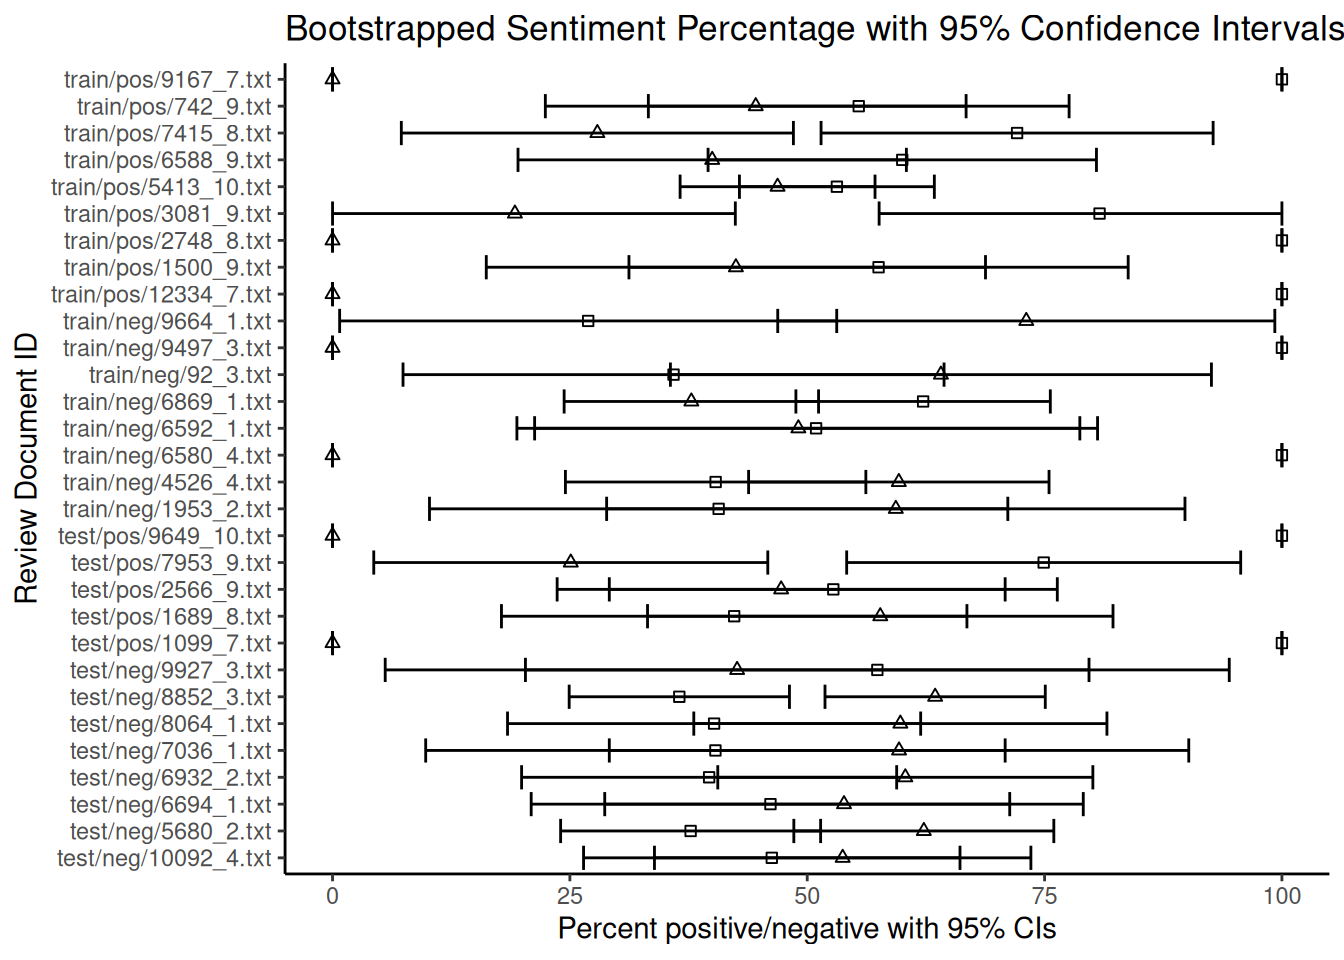
\includegraphics[keepaspectratio]{Introduction-to-Quantitative-Text-Analysis_files/figure-latex/ggplot-moviereviews-posneg-1.pdf}}

Note that the fact that some documents are shorter than others and contain fewer dictionary words introduces more uncertainty to the estimates of the percentages. As can be seen from the overlapping confidence intervals for many documents, the estimated rate of negative words is not statistically different from that of positive words at the 95\% confidence level for these reviews. Based on this dictionary and bootstrapping method, the sentiment for these reviews appears to be mixed or uncertain. The width of the error bars provides a visual indication of this uncertainty for each document. While bootstrapping quantifies this uncertainty, its interpretation requires careful consideration of the underlying assumptions.

\subsection{Twitter}\label{twitter}

Now, let us turn to another example of sentiment analysis using Twitter/X data. Due to its informal nature and use of slang, hashtags and emoticons, this type of text presents unique challenges, especially when cleaning. Here, we examine sentiment towards several major US airlines based on a dataset of tweets. In this case, researchers scraped data from Twitter and asked participants to classify the sentiment of each tweet as negative, positive or neutral, and if negative, to explain why. The data also includes information about the coders' confidence levels, the airline in question and the tweets' metadata. We can download this data from platforms such as Kaggle (e.g.~the `Airline Sentiment' dataset), but for ease of use in this example, we will load it directly from GitHub via a URL:

\begin{Shaded}
\begin{Highlighting}[]
\NormalTok{urlfile }\OtherTok{=} \StringTok{"https://raw.githubusercontent.com/SCJBruinsma/qta{-}files/master/Tweets.csv"}
\NormalTok{tweets }\OtherTok{\textless{}{-}} \FunctionTok{read.csv}\NormalTok{(}\FunctionTok{url}\NormalTok{(urlfile), }\AttributeTok{stringsAsFactors =} \ConstantTok{FALSE}\NormalTok{)  }\CommentTok{\# Use stringsAsFactors = FALSE to keep text as character}
\FunctionTok{head}\NormalTok{(tweets)}
\end{Highlighting}
\end{Shaded}

\begin{verbatim}
##       tweet_id airline_sentiment airline_sentiment_confidence negativereason
## 1 5.703061e+17           neutral                       1.0000               
## 2 5.703011e+17          positive                       0.3486               
## 3 5.703011e+17           neutral                       0.6837               
## 4 5.703010e+17          negative                       1.0000     Bad Flight
## 5 5.703008e+17          negative                       1.0000     Can't Tell
## 6 5.703008e+17          negative                       1.0000     Can't Tell
##   negativereason_confidence        airline airline_sentiment_gold       name
## 1                        NA Virgin America                           cairdin
## 2                    0.0000 Virgin America                          jnardino
## 3                        NA Virgin America                        yvonnalynn
## 4                    0.7033 Virgin America                          jnardino
## 5                    1.0000 Virgin America                          jnardino
## 6                    0.6842 Virgin America                          jnardino
##   negativereason_gold retweet_count
## 1                                 0
## 2                                 0
## 3                                 0
## 4                                 0
## 5                                 0
## 6                                 0
##                                                                                                                                       text
## 1                                                                                                      @VirginAmerica What @dhepburn said.
## 2                                                                 @VirginAmerica plus you've added commercials to the experience... tacky.
## 3                                                                  @VirginAmerica I didn't today... Must mean I need to take another trip!
## 4           @VirginAmerica it's really aggressive to blast obnoxious "entertainment" in your guests' faces &amp; they have little recourse
## 5                                                                                  @VirginAmerica and it's a really big bad thing about it
## 6 @VirginAmerica seriously would pay $30 a flight for seats that didn't have this playing.\nit's really the only bad thing about flying VA
##   tweet_coord             tweet_created tweet_location
## 1             2015-02-24 11:35:52 -0800               
## 2             2015-02-24 11:15:59 -0800               
## 3             2015-02-24 11:15:48 -0800      Lets Play
## 4             2015-02-24 11:15:36 -0800               
## 5             2015-02-24 11:14:45 -0800               
## 6             2015-02-24 11:14:33 -0800               
##                user_timezone
## 1 Eastern Time (US & Canada)
## 2 Pacific Time (US & Canada)
## 3 Central Time (US & Canada)
## 4 Pacific Time (US & Canada)
## 5 Pacific Time (US & Canada)
## 6 Pacific Time (US & Canada)
\end{verbatim}

After cleaning the text data in the data frame, we transform it into a \texttt{quanteda} corpus object, specifying that our text is in the \texttt{text} field. We then proceed with the standard \texttt{quanteda} preprocessing steps: transforming our corpus into a tokens object and removing stop words:

\begin{Shaded}
\begin{Highlighting}[]
\NormalTok{corpus\_tweets }\OtherTok{\textless{}{-}} \FunctionTok{corpus}\NormalTok{(tweets, }\AttributeTok{text\_field =} \StringTok{"text"}\NormalTok{)}

\NormalTok{data\_tweets\_tokens }\OtherTok{\textless{}{-}} \FunctionTok{tokens}\NormalTok{(corpus\_tweets, }\AttributeTok{remove\_punct =} \ConstantTok{TRUE}\NormalTok{, }\AttributeTok{remove\_symbols =} \ConstantTok{TRUE}\NormalTok{,}
    \AttributeTok{remove\_numbers =} \ConstantTok{TRUE}\NormalTok{, }\AttributeTok{remove\_url =} \ConstantTok{TRUE}\NormalTok{, }\AttributeTok{remove\_separators =} \ConstantTok{TRUE}\NormalTok{, }\AttributeTok{split\_hyphens =} \ConstantTok{FALSE}\NormalTok{,}
    \AttributeTok{split\_tags =} \ConstantTok{FALSE}\NormalTok{)}

\NormalTok{data\_tweets\_tokens }\OtherTok{\textless{}{-}} \FunctionTok{tokens\_select}\NormalTok{(data\_tweets\_tokens, }\FunctionTok{stopwords}\NormalTok{(}\StringTok{"english"}\NormalTok{), }\AttributeTok{selection =} \StringTok{"remove"}\NormalTok{)}

\NormalTok{data\_tweets\_dfm }\OtherTok{\textless{}{-}} \FunctionTok{dfm}\NormalTok{(data\_tweets\_tokens)}
\end{Highlighting}
\end{Shaded}

Now, we can apply our sentiment dictionary. As discussed earlier, we can do this in two ways: by applying it to the dfm using \texttt{dfm\_lookup()} or to the tokens object using \texttt{tokens\_lookup()}. Both should give similar results for single-word entries, but we have to use \texttt{tokens\_lookup()} to correctly identify multi-word expressions. As the LSD2015 dictionary contains some multi-word expressions, using \texttt{tokens\_lookup()} and then converting the result to a dfm is the preferred approach to ensure that all dictionary entries are captured:

\begin{Shaded}
\begin{Highlighting}[]
\NormalTok{results\_tokens }\OtherTok{\textless{}{-}} \FunctionTok{tokens\_lookup}\NormalTok{(data\_tweets\_tokens, data\_dictionary\_LSD2015)}

\CommentTok{\# Convert the resulting tokens object (with categories) to a dfm}
\NormalTok{results\_dfm }\OtherTok{\textless{}{-}} \FunctionTok{dfm}\NormalTok{(results\_tokens)}

\CommentTok{\# Convert the dfm to a data frame for analysis}
\NormalTok{results\_df }\OtherTok{\textless{}{-}} \FunctionTok{convert}\NormalTok{(results\_dfm, }\AttributeTok{to =} \StringTok{"data.frame"}\NormalTok{)}
\end{Highlighting}
\end{Shaded}

Now, let us see how well our dictionary-based sentiment matches the human-assigned sentiment labels in the original dataset. We recode the human-assigned \texttt{airline\_sentiment} labels from our original dataset into numerical values for easier comparison (e.g.~positive = 1, negative = -1, neutral = 0):

\begin{Shaded}
\begin{Highlighting}[]
\FunctionTok{library}\NormalTok{(car)}

\NormalTok{labels }\OtherTok{\textless{}{-}}\NormalTok{ tweets}\SpecialCharTok{$}\NormalTok{airline\_sentiment}
\NormalTok{sentiment\_numeric }\OtherTok{\textless{}{-}}\NormalTok{ car}\SpecialCharTok{::}\FunctionTok{recode}\NormalTok{(labels, }\StringTok{"\textquotesingle{}positive\textquotesingle{}=1; \textquotesingle{}negative\textquotesingle{}={-}1; \textquotesingle{}neutral\textquotesingle{}=0"}\NormalTok{)}
\FunctionTok{print}\NormalTok{(}\FunctionTok{table}\NormalTok{(sentiment\_numeric))}
\end{Highlighting}
\end{Shaded}

A quick look at the table shows how human-assigned sentiment is distributed. Perhaps not unexpected, negative tweets about airlines are more common than positive ones. We now want to combine this data with the output of our dictionary analysis to calculate an overall sentiment score for each tweet. One common method is subtracting the negative score from the positive score (positive minus negative). A higher resulting score indicates a more positive dictionary-based sentiment:

\begin{Shaded}
\begin{Highlighting}[]
\NormalTok{comparison\_df }\OtherTok{\textless{}{-}} \FunctionTok{as.data.frame}\NormalTok{(}\FunctionTok{cbind}\NormalTok{(results\_df}\SpecialCharTok{$}\NormalTok{positive, results\_df}\SpecialCharTok{$}\NormalTok{negative, sentiment\_numeric))}
\FunctionTok{names}\NormalTok{(comparison\_df) }\OtherTok{\textless{}{-}} \FunctionTok{c}\NormalTok{(}\StringTok{"positive\_dict"}\NormalTok{, }\StringTok{"negative\_dict"}\NormalTok{, }\StringTok{"human\_sentiment"}\NormalTok{)}

\CommentTok{\# Calculate the sentiment difference from dictionary counts}
\NormalTok{comparison\_df}\SpecialCharTok{$}\NormalTok{sentiment\_difference\_dict }\OtherTok{\textless{}{-}}\NormalTok{ comparison\_df}\SpecialCharTok{$}\NormalTok{positive\_dict }\SpecialCharTok{{-}}\NormalTok{ comparison\_df}\SpecialCharTok{$}\NormalTok{negative\_dict}

\FunctionTok{head}\NormalTok{(comparison\_df)}
\end{Highlighting}
\end{Shaded}

\begin{verbatim}
##   positive_dict negative_dict human_sentiment sentiment_difference_dict
## 1             0             0               0                         0
## 2             0             1               1                        -1
## 3             0             0               0                         0
## 4             1             3              -1                        -2
## 5             0             1              -1                        -1
## 6             0             1              -1                        -1
\end{verbatim}

Finally, we can visualise the relationship between human-assigned and dictionary-based sentiment scores using a scatter plot. Since human sentiment is categorical (or comprises a small set of numerical values), adding jitter to the scores can help to visualise density. A simple linear regression line can illustrate the overall trend. We will use the results from the \texttt{tokens\_lookup()} function, as this handles multi-word expressions correctly.

\begin{Shaded}
\begin{Highlighting}[]
\FunctionTok{library}\NormalTok{(ggplot2)}

\FunctionTok{ggplot}\NormalTok{(comparison\_df,}
       \FunctionTok{aes}\NormalTok{(}\AttributeTok{x =}\NormalTok{ sentiment\_difference\_dict, }\AttributeTok{y =}\NormalTok{ human\_sentiment)) }\SpecialCharTok{+}
  \FunctionTok{geom\_jitter}\NormalTok{(}\AttributeTok{shape =} \DecValTok{1}\NormalTok{, }\AttributeTok{alpha =} \FloatTok{0.5}\NormalTok{) }\SpecialCharTok{+} \CommentTok{\# Add jitter and transparency}
  \FunctionTok{geom\_smooth}\NormalTok{(}\AttributeTok{method =}\NormalTok{ lm, }\AttributeTok{se =} \ConstantTok{FALSE}\NormalTok{) }\SpecialCharTok{+} \CommentTok{\# Add linear regression line}
  \FunctionTok{scale\_x\_continuous}\NormalTok{(}\AttributeTok{name =} \StringTok{"Dictionary Sentiment Score (Positive {-} Negative)"}\NormalTok{) }\SpecialCharTok{+}
  \FunctionTok{scale\_y\_continuous}\NormalTok{(}\AttributeTok{name =} \StringTok{"Human Judgment (Recoded)"}\NormalTok{) }\SpecialCharTok{+}
  \FunctionTok{ggtitle}\NormalTok{(}\StringTok{"Dictionary Sentiment vs. Human Judgment for Tweets"}\NormalTok{) }\SpecialCharTok{+}
  \FunctionTok{theme\_classic}\NormalTok{()}
\end{Highlighting}
\end{Shaded}

\pandocbounded{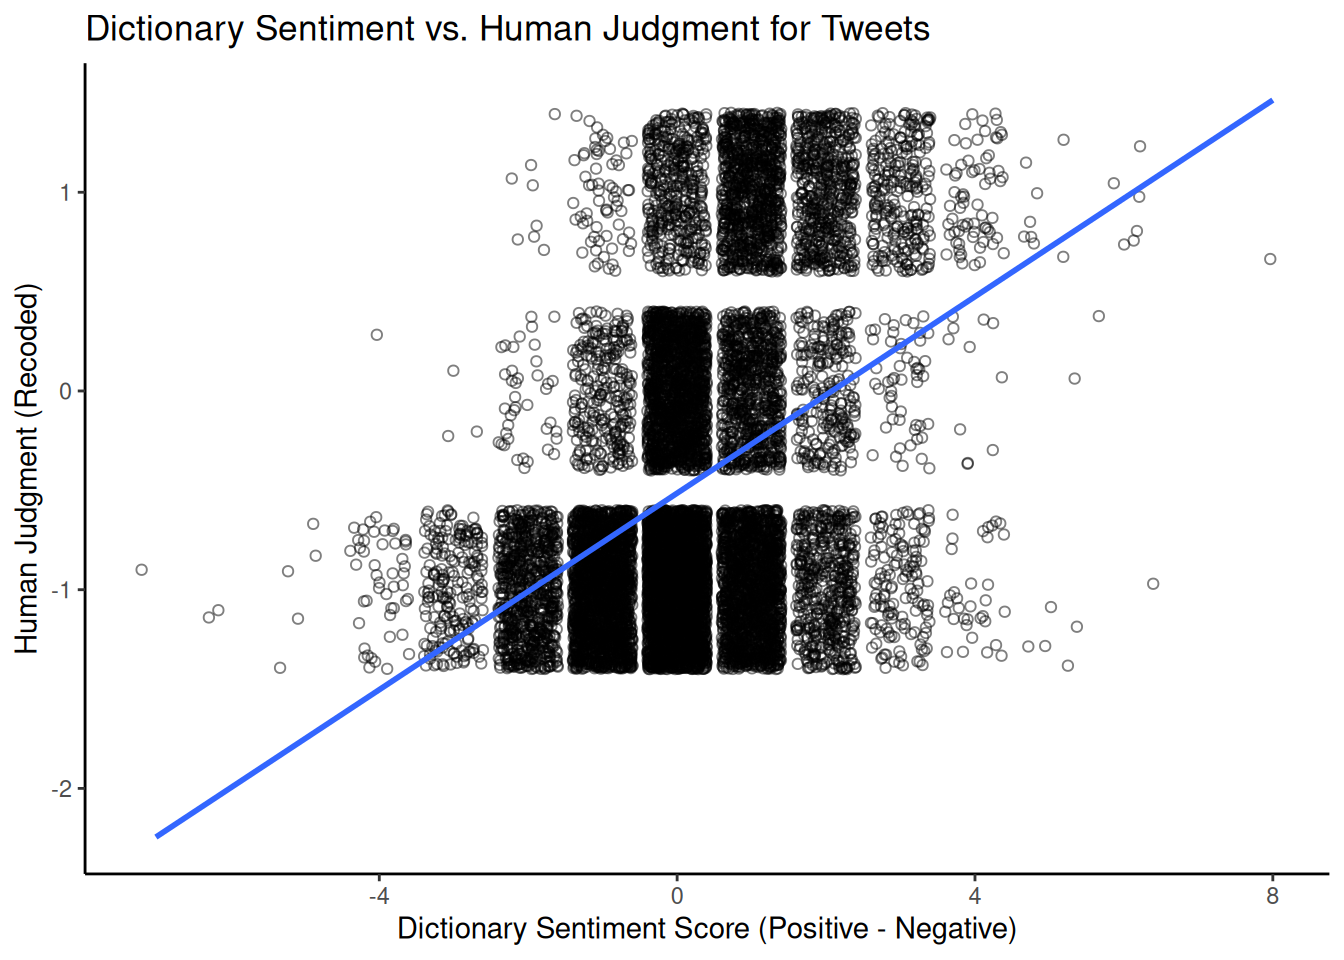
\includegraphics[keepaspectratio]{Introduction-to-Quantitative-Text-Analysis_files/figure-latex/ggplot-tweets-comparison-1.pdf}}

This graph visually shows the correlation between dictionary-based and human-assigned sentiment scores. A positive slope suggests that human coders rate tweets with higher positive-minus-negative dictionary scores as more positive. The strength of this relationship (e.g., measured by the correlation coefficient or \(R^2\) from the linear model) indicates how well the dictionary captures the sentiment as perceived by humans in that particular domain.

\subsection{VADER}\label{vader}

Another popular dictionary-based approach for sentiment analysis in social media contexts is VADER (\citeproc{ref-Hutto2014a}{Hutto \& Gilbert, 2014}) (Valence Aware Dictionary and sEntiment Reasoner). Unlike a simple dictionary lookup, VADER is a rule-based model that considers punctuation, capitalisation, emojis, and negation to determine sentiment intensity. It provides a continuous sentiment score ranging from -1 (most negative) to +1 (most positive) and scores for the proportions of positive, negative and neutral sentiment. Unlike most dictionaries, which rely on the judgement of a single expert or small group, the VADER dictionary was developed and validated using crowdsourced human judgements.

We can use the \texttt{vader} package to use VADER in R; let's test it again using the airline tweet data. First, we reload the data and select a subset of tweets to work with to speed up processing, converting the text into a character vector:

\begin{Shaded}
\begin{Highlighting}[]
\NormalTok{urlfile }\OtherTok{=} \StringTok{"https://raw.githubusercontent.com/SCJBruinsma/qta{-}files/master/Tweets.csv"}
\NormalTok{tweets\_vader }\OtherTok{\textless{}{-}} \FunctionTok{read.csv}\NormalTok{(}\FunctionTok{url}\NormalTok{(urlfile), }\AttributeTok{stringsAsFactors =} \ConstantTok{FALSE}\NormalTok{)}
\CommentTok{\# Select a sample of 1000 tweets for demonstration}
\FunctionTok{set.seed}\NormalTok{(}\DecValTok{42}\NormalTok{)}
\NormalTok{tweets\_sample\_vader }\OtherTok{\textless{}{-}}\NormalTok{ tweets\_vader[}\FunctionTok{sample}\NormalTok{(}\FunctionTok{nrow}\NormalTok{(tweets\_vader), }\DecValTok{1000}\NormalTok{), ]}
\NormalTok{text\_vader }\OtherTok{\textless{}{-}}\NormalTok{ tweets\_sample\_vader}\SpecialCharTok{$}\NormalTok{text  }\CommentTok{\# Extract the text column}
\end{Highlighting}
\end{Shaded}

We then apply VADER to our tweets using the \texttt{vader\_df()} function, which is designed to work with a character vector or data frame of text.

\begin{Shaded}
\begin{Highlighting}[]
\FunctionTok{library}\NormalTok{(vader)}

\NormalTok{results\_vader }\OtherTok{\textless{}{-}} \FunctionTok{vader\_df}\NormalTok{(text\_vader)  }\CommentTok{\# Apply vader\_df to the extracted text vector}
\end{Highlighting}
\end{Shaded}

VADER then provides us with a data frame consisting of several variables. The most important ones are:

\begin{itemize}
\tightlist
\item
  \texttt{text}: The original text of the tweet.
\item
  \texttt{compound}: A single, aggregated sentiment score ranging from -1 to +1. This is often the primary score we would use
\item
  \texttt{pos}, \texttt{neg}, \texttt{neu}: The proportion of the text that falls into positive, negative, and neutral categories, respectively.
\item
  \texttt{word\_scores}: (If requested) Individual sentiment scores for each word.
\end{itemize}

To get a better idea of the output, we can look at the distribution of the \texttt{compound} sentiment scores using a histogram:

\begin{Shaded}
\begin{Highlighting}[]
\FunctionTok{library}\NormalTok{(ggplot2)}

\FunctionTok{ggplot}\NormalTok{(}\AttributeTok{data =}\NormalTok{ results\_vader, }\FunctionTok{aes}\NormalTok{(}\AttributeTok{x =}\NormalTok{ compound)) }\SpecialCharTok{+} \FunctionTok{geom\_histogram}\NormalTok{(}\AttributeTok{bins =} \DecValTok{30}\NormalTok{) }\SpecialCharTok{+} \FunctionTok{scale\_x\_continuous}\NormalTok{(}\AttributeTok{name =} \StringTok{"Compound Sentiment Score"}\NormalTok{,}
    \AttributeTok{expand =} \FunctionTok{c}\NormalTok{(}\DecValTok{0}\NormalTok{, }\DecValTok{0}\NormalTok{)) }\SpecialCharTok{+} \FunctionTok{scale\_y\_continuous}\NormalTok{(}\AttributeTok{name =} \StringTok{"Frequency"}\NormalTok{, }\AttributeTok{expand =} \FunctionTok{c}\NormalTok{(}\DecValTok{0}\NormalTok{, }\DecValTok{0}\NormalTok{)) }\SpecialCharTok{+}
    \FunctionTok{ggtitle}\NormalTok{(}\StringTok{"Distribution of VADER Compound Sentiment Scores"}\NormalTok{) }\SpecialCharTok{+} \FunctionTok{theme\_classic}\NormalTok{()}
\end{Highlighting}
\end{Shaded}

\pandocbounded{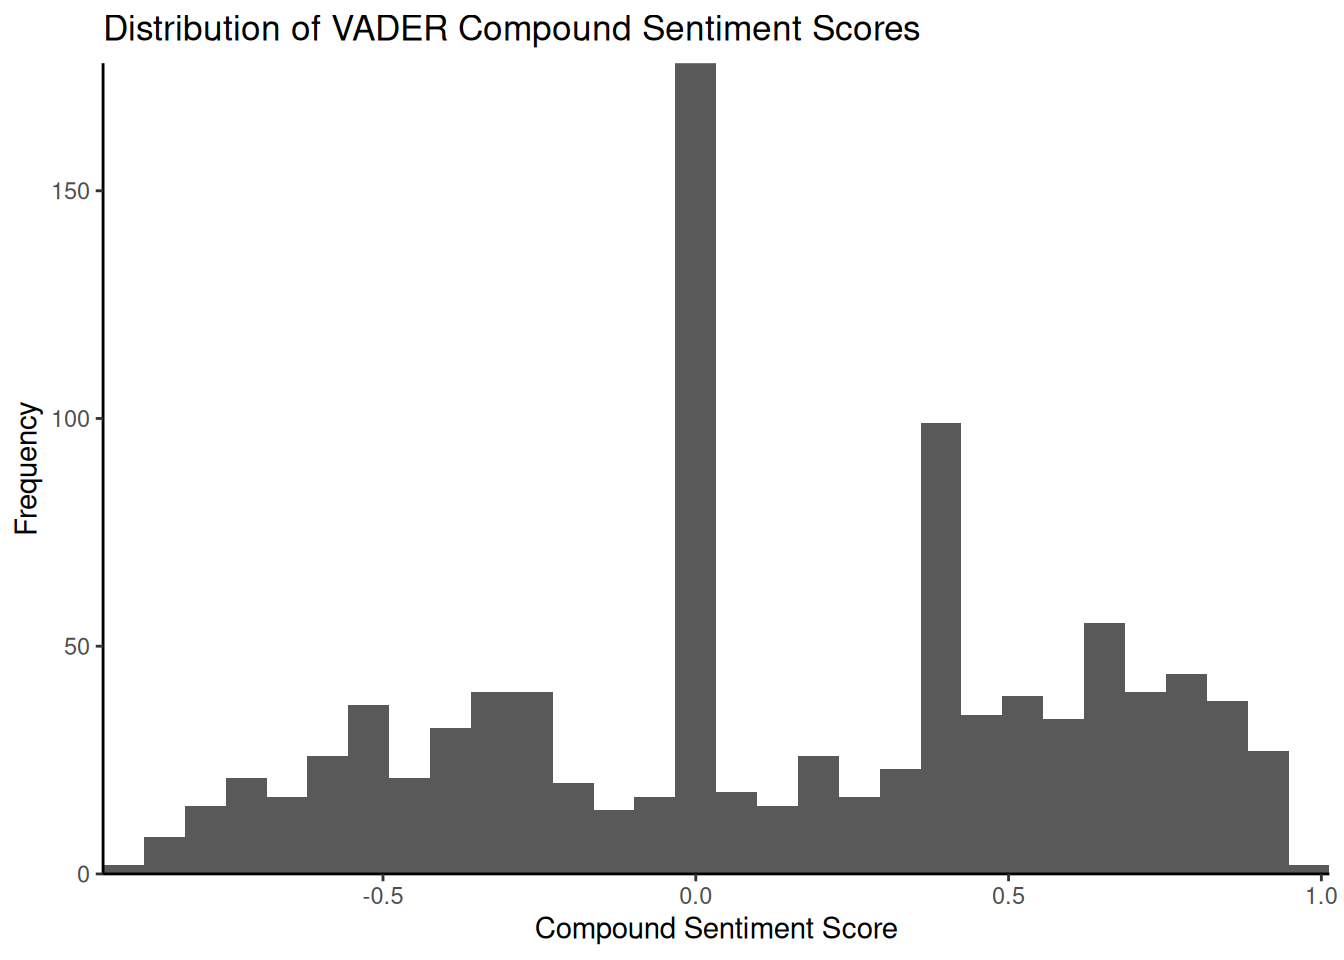
\includegraphics[keepaspectratio]{Introduction-to-Quantitative-Text-Analysis_files/figure-latex/tweets-vader-outputs-1.pdf}}

The histogram illustrates the frequency of tweets across the range of composite sentiment scores. In this dataset, a significant proportion of tweets tend to cluster around a neutral score (\(0\)), potentially due to the presence of purely informative tweets or the absence of strong emotional language. Examining tweets with scores close to zero can help us understand why they are classified as neutral by VADER. Tweets such as `@JetBlue Counting on your flight \(989\) to get to DC!' may lack explicit positive or negative language and, therefore, receive a neutral or near-neutral composite score. As before, we can compare the VADER composite score with the human-assigned sentiment labels:

\begin{Shaded}
\begin{Highlighting}[]
\NormalTok{vader\_comparison\_df }\OtherTok{\textless{}{-}} \FunctionTok{data.frame}\NormalTok{(}\AttributeTok{vader\_compound =}\NormalTok{ results\_vader}\SpecialCharTok{$}\NormalTok{compound, }\AttributeTok{human\_sentiment =}\NormalTok{ sentiment\_numeric[}\FunctionTok{as.numeric}\NormalTok{(}\FunctionTok{rownames}\NormalTok{(tweets\_sample\_vader))])}

\NormalTok{vader\_comparison\_df }\OtherTok{\textless{}{-}} \FunctionTok{na.omit}\NormalTok{(vader\_comparison\_df)}

\FunctionTok{ggplot}\NormalTok{(vader\_comparison\_df, }\FunctionTok{aes}\NormalTok{(}\AttributeTok{x =}\NormalTok{ vader\_compound, }\AttributeTok{y =}\NormalTok{ human\_sentiment)) }\SpecialCharTok{+}
    \FunctionTok{geom\_jitter}\NormalTok{(}\AttributeTok{shape =} \DecValTok{1}\NormalTok{, }\AttributeTok{alpha =} \FloatTok{0.5}\NormalTok{) }\SpecialCharTok{+} \CommentTok{\# Add jitter and transparency}
    \FunctionTok{geom\_smooth}\NormalTok{(}\AttributeTok{method =}\NormalTok{ lm, }\AttributeTok{se =} \ConstantTok{FALSE}\NormalTok{) }\SpecialCharTok{+} \CommentTok{\# Add linear regression line}
    \FunctionTok{scale\_x\_continuous}\NormalTok{(}\AttributeTok{name =} \StringTok{"VADER Compound Sentiment Score"}\NormalTok{) }\SpecialCharTok{+}
    \FunctionTok{scale\_y\_continuous}\NormalTok{(}\AttributeTok{name =} \StringTok{"Human Judgment (Recoded)"}\NormalTok{) }\SpecialCharTok{+}
    \FunctionTok{ggtitle}\NormalTok{(}\StringTok{"VADER Compound Sentiment vs. Human Judgment for Tweets"}\NormalTok{) }\SpecialCharTok{+}
    \FunctionTok{theme\_classic}\NormalTok{()}
\end{Highlighting}
\end{Shaded}

\begin{verbatim}
## `geom_smooth()` using formula = 'y ~ x'
\end{verbatim}

\pandocbounded{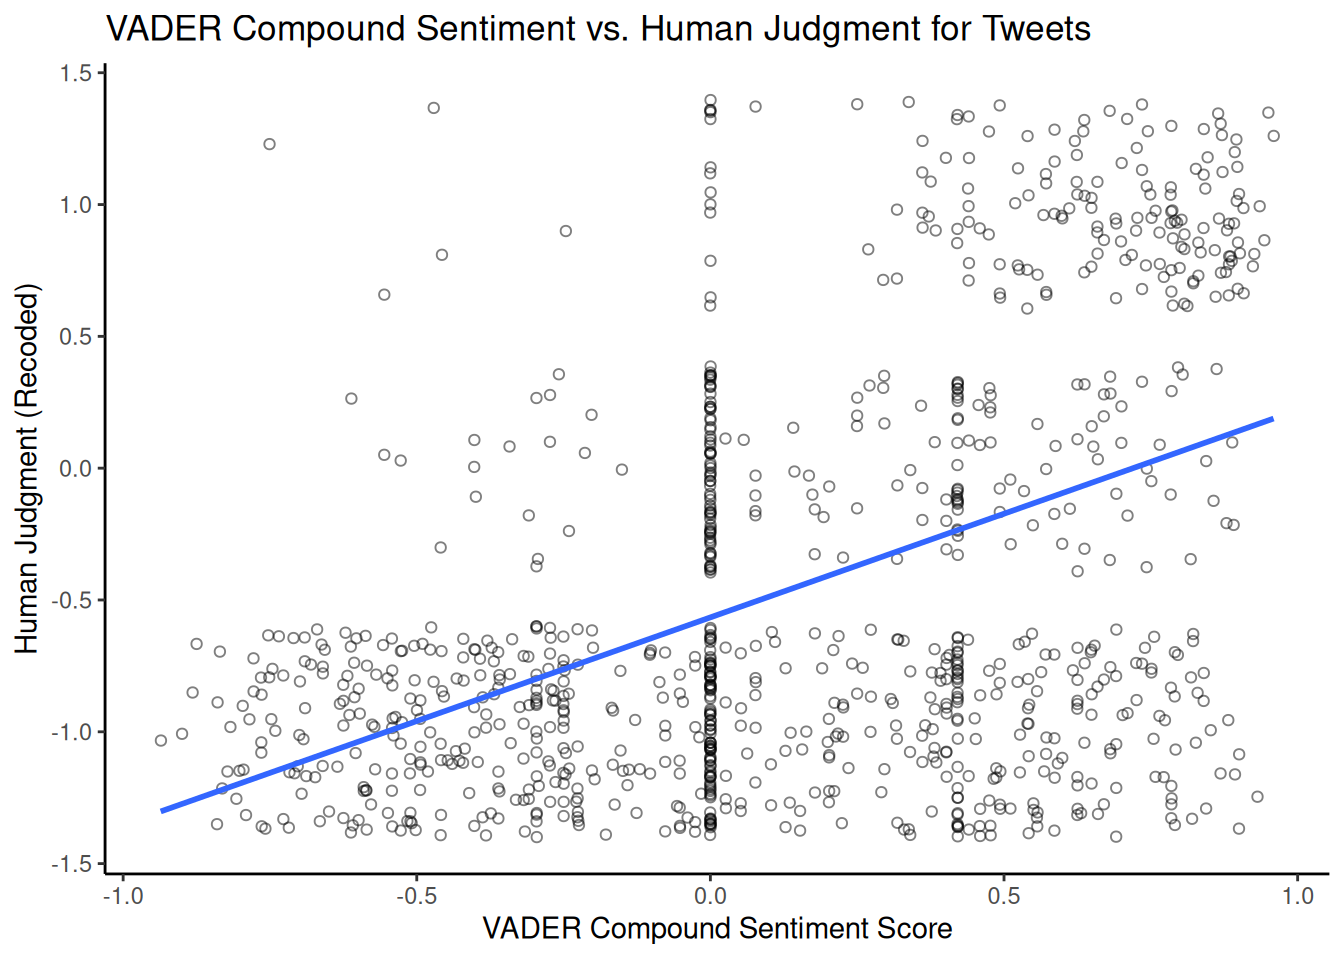
\includegraphics[keepaspectratio]{Introduction-to-Quantitative-Text-Analysis_files/figure-latex/tweets-vader-comparison-1.pdf}}

Comparing this plot with the previous one using LSD2015 provides us with some additional insight into which dictionary/approach better matches human judgement for this dataset.

\section{Exercises}\label{exercises-1}

\begin{enumerate}
\def\labelenumi{\arabic{enumi}.}
\item
  Using a sentiment analysis dictionary such as LSD2015, analyse the sentiment expressed in the Wikipedia article on the Cold War from the previous chapter. Are there differences in sentiment between the paragraphs, and if so, what might the reasons for these differences be? Consider plotting the sentiment score against the document index.
\item
  How did the Cold War influence culture, as reflected in textual data? Create your own dictionary of words or phrases representing cultural aspects influenced by the Cold War (e.g.~terms related to fear, propaganda and specific cultural phenomena). Apply this dictionary to a relevant corpus (e.g.~articles about the Cold War or cultural texts from the period) and analyse the frequency of these terms. Discuss your findings based on the dictionary counts.
\item
  Explore the different sentiment scores provided by the \texttt{vader} package (pos, neg, neu and compound). Plot the distribution of the `pos', `neg' and `neu' scores. How do these relate to the `compound' score and the human-assigned labels?
\item
  Research other sentiment dictionaries available in R, for example, in packages such as \texttt{syuzhet} or \texttt{tidytext} that can work with \texttt{quanteda} outputs. Apply one of these dictionaries to the film review or tweet data, then compare the results with those obtained using LSD2015 or VADER. What similarities and differences are there in the sentiment scores?
\item
  Consider the limitations of dictionary analysis, especially with regard to context and negation. Find examples in the tweet data where a simple dictionary lookup might misclassify the sentiment due to negation (`not happy') or sarcasm. How might these cases be handled in a more advanced approach to sentiment analysis?
\end{enumerate}

\chapter{Scaling Methods}\label{scaling}

While methods like dictionary analysis help identify themes or sentiments, their dictionary categories are often treated as distinct and not inherently ordered on a scale. If we want to compare texts or place them along a continuum (e.g., a left-right political spectrum, a scale of formality, or a sentiment dimension), we need methods to place documents on a scale.

In this chapter, we will look at three prominent scaling methods: \emph{Wordscores} (\citeproc{ref-Laver2003a}{Laver et al., 2003}), \emph{Wordfish} (\citeproc{ref-Slapin2008a}{Slapin \& Proksch, 2008}) and \emph{Correspondence Analysis} (specifically Multiple Correspondence Analysis for categorical text data). The first two were initially part of the main \texttt{quanteda} package but have since moved to the \texttt{quanteda.textmodels} package. Correspondence Analysis, meanwhile, is a dimensionality reduction technique that can position documents and features in a multidimensional space and reveal relationships between them. For this, we will mainly use functions from the \texttt{FactoMineR} and \texttt{factoextra} packages, but we will also look at the \texttt{textmodel\_ca} from \texttt{quanteda.textmodels}.

\section{Wordscores}\label{wordscores}

Wordscores is a supervised scaling method that requires a set of \emph{reference texts} for which the position on the scale of interest is already known. These positions are then used to estimate scores for individual words, which are aggregated to estimate the position of new texts (for which the position is unknown) on the same scale. The basic idea is that words that frequently appear in texts with known extreme positions on a scale are likely to indicate that position. For instance, words that frequently appear in texts known to be on the far left of the scale might receive low scores, while words that frequently appear in texts on the far right might receive high scores. The score of a new text is calculated by taking the weighted average of the scores of the words it contains, where the weights are usually the word frequencies.

Here, we aim to position the 2005 manifestos of the five main UK political parties (Labour, Liberal Democrats, Conservatives, Scottish National Party and Plaid Cymru) on a general left-right scale. The 2001 manifestos of the same parties are used as reference texts. We will use external ratings, such as those from the 2002 Chapel Hill Expert Survey (\citeproc{ref-Bakker2012a}{Bakker et al., 2012}) or other expert judgements, to determine their positions on the scale.

First, we load the necessary libraries and the corpus of UK party manifestos provided in \texttt{quanteda.corpora}. We then subset the corpus to include only the 2001 and 2005 manifestos of the selected parties. We then create a document feature matrix (DFM) following standard preprocessing steps.

\begin{Shaded}
\begin{Highlighting}[]
\FunctionTok{library}\NormalTok{(quanteda)}
\FunctionTok{library}\NormalTok{(quanteda.corpora)}
\FunctionTok{library}\NormalTok{(dplyr)  }\CommentTok{\# For data manipulation}
\FunctionTok{library}\NormalTok{(stringr)  }\CommentTok{\# For string manipulation}
\FunctionTok{library}\NormalTok{(ggplot2)  }\CommentTok{\# For plotting}

\CommentTok{\# Load the UK manifestos corpus}
\FunctionTok{data}\NormalTok{(data\_corpus\_ukmanifestos)}

\NormalTok{corpus\_manifestos }\OtherTok{\textless{}{-}} \FunctionTok{corpus\_subset}\NormalTok{(data\_corpus\_ukmanifestos, Year }\SpecialCharTok{\%in\%} \FunctionTok{c}\NormalTok{(}\DecValTok{2001}\NormalTok{, }\DecValTok{2005}\NormalTok{))}
\NormalTok{corpus\_manifestos }\OtherTok{\textless{}{-}} \FunctionTok{corpus\_subset}\NormalTok{(corpus\_manifestos, Party }\SpecialCharTok{\%in\%} \FunctionTok{c}\NormalTok{(}\StringTok{"Lab"}\NormalTok{, }\StringTok{"LD"}\NormalTok{, }\StringTok{"Con"}\NormalTok{,}
    \StringTok{"SNP"}\NormalTok{, }\StringTok{"PCy"}\NormalTok{))}

\CommentTok{\# Tokenise the corpus with standard preprocessing}
\NormalTok{data\_manifestos\_tokens }\OtherTok{\textless{}{-}} \FunctionTok{tokens}\NormalTok{(corpus\_manifestos, }\AttributeTok{what =} \StringTok{"word"}\NormalTok{, }\AttributeTok{remove\_punct =} \ConstantTok{TRUE}\NormalTok{,}
    \AttributeTok{remove\_symbols =} \ConstantTok{TRUE}\NormalTok{, }\AttributeTok{remove\_numbers =} \ConstantTok{TRUE}\NormalTok{, }\AttributeTok{remove\_url =} \ConstantTok{TRUE}\NormalTok{, }\AttributeTok{remove\_separators =} \ConstantTok{TRUE}\NormalTok{,}
    \AttributeTok{split\_hyphens =} \ConstantTok{FALSE}\NormalTok{, }\AttributeTok{include\_docvars =} \ConstantTok{TRUE}\NormalTok{, }\AttributeTok{padding =} \ConstantTok{FALSE}\NormalTok{)}

\NormalTok{data\_manifestos\_tokens }\OtherTok{\textless{}{-}} \FunctionTok{tokens\_tolower}\NormalTok{(data\_manifestos\_tokens)}
\NormalTok{data\_manifestos\_tokens }\OtherTok{\textless{}{-}} \FunctionTok{tokens\_select}\NormalTok{(data\_manifestos\_tokens, }\FunctionTok{stopwords}\NormalTok{(}\StringTok{"english"}\NormalTok{),}
    \AttributeTok{selection =} \StringTok{"remove"}\NormalTok{)}

\NormalTok{data\_manifestos\_dfm }\OtherTok{\textless{}{-}} \FunctionTok{dfm}\NormalTok{(data\_manifestos\_tokens)}

\CommentTok{\# Print the document names to verify the order}
\NormalTok{data\_manifestos\_dfm}\SpecialCharTok{@}\NormalTok{Dimnames}\SpecialCharTok{$}\NormalTok{docs}
\end{Highlighting}
\end{Shaded}

\begin{verbatim}
##  [1] "UK_natl_2001_en_Con" "UK_natl_2001_en_Lab" "UK_natl_2001_en_LD" 
##  [4] "UK_natl_2001_en_PCy" "UK_natl_2001_en_SNP" "UK_natl_2005_en_Con"
##  [7] "UK_natl_2005_en_Lab" "UK_natl_2005_en_LD"  "UK_natl_2005_en_PCy"
## [10] "UK_natl_2005_en_SNP"
\end{verbatim}

The order of the documents in the DFM is essential for assigning reference scores. We can check this by looking at the document names. Next, we set the known scores (from the 2002 Chapel Hill Expert Survey) for the reference texts (the 2001 manifestos). We set the score to `NA' for the new texts (the 2005 manifestos). These scores should match the order of the documents in the DFM. Finally, we run the \texttt{textmodel\_wordscores()} function, providing it with the DFM and the vector of reference scores:

\begin{Shaded}
\begin{Highlighting}[]
\FunctionTok{library}\NormalTok{(quanteda.textmodels)}

\NormalTok{scores }\OtherTok{\textless{}{-}} \FunctionTok{c}\NormalTok{(}\FloatTok{7.7}\NormalTok{, }\FloatTok{5.2}\NormalTok{, }\FloatTok{3.8}\NormalTok{, }\FloatTok{3.2}\NormalTok{, }\DecValTok{3}\NormalTok{, }\ConstantTok{NA}\NormalTok{, }\ConstantTok{NA}\NormalTok{, }\ConstantTok{NA}\NormalTok{, }\ConstantTok{NA}\NormalTok{, }\ConstantTok{NA}\NormalTok{)}

\CommentTok{\# Run the Wordscores model}
\NormalTok{ws }\OtherTok{\textless{}{-}} \FunctionTok{textmodel\_wordscores}\NormalTok{(data\_manifestos\_dfm, scores)}

\CommentTok{\# Display the summary of the Wordscores model, including word scores}
\FunctionTok{summary}\NormalTok{(ws)}
\end{Highlighting}
\end{Shaded}

\begin{verbatim}
## 
## Call:
## textmodel_wordscores.dfm(x = data_manifestos_dfm, y = scores)
## 
## Reference Document Statistics:
##                     score total min max   mean median
## UK_natl_2001_en_Con   7.7  7179   0  92 0.8646      0
## UK_natl_2001_en_Lab   5.2 16386   0 166 1.9735      0
## UK_natl_2001_en_LD    3.8 12338   0 101 1.4860      0
## UK_natl_2001_en_PCy   3.2  3508   0  72 0.4225      0
## UK_natl_2001_en_SNP   3.0  5692   0 108 0.6855      0
## UK_natl_2005_en_Con    NA  4349   0  46 0.5238      0
## UK_natl_2005_en_Lab    NA 13366   0 147 1.6098      0
## UK_natl_2005_en_LD     NA  9263   0 109 1.1156      0
## UK_natl_2005_en_PCy    NA  4203   0 148 0.5062      0
## UK_natl_2005_en_SNP    NA  1508   0  49 0.1816      0
## 
## Wordscores:
## (showing first 30 elements)
##         time       common        sense conservative    manifesto introduction 
##        5.828        6.525        7.359        7.143        4.475        3.979 
##        lives      raising       family       living       safely      earning 
##        6.034        4.423        5.513        4.717        5.738        6.034 
##      staying      healthy      growing        older      knowing        world 
##        6.938        4.289        4.741        6.276        7.700        4.365 
##       leader     stronger      society         town      country    civilised 
##        4.520        4.904        4.338        7.499        4.397        4.272 
##        proud    democracy   conclusion      present    ambitious    programme 
##        6.064        5.255        6.938        3.589        4.468        4.230
\end{verbatim}

The \texttt{summary()} output shows the estimated score for each word based on its distribution across the reference texts. These are the ``word scores.'' A text's score is a weighted average of these word scores. Wordscores also calculates a raw score for each text. However, these raw scores are often clustered around the mean. To make the virgin text scores comparable to the reference scale, a \emph{rescaling} step is applied. \texttt{predict()} with a \texttt{textmodel\_wordscores} object performs this rescaling. There are two standard rescaling methods:

\begin{enumerate}
\def\labelenumi{\arabic{enumi}.}
\tightlist
\item
  \textbf{LBG (Laver--Benoit--Garry)} (\citeproc{ref-Laver2003a}{Laver et al., 2003}): Rescales the raw scores linearly to match the range of the reference scores.
\item
  \textbf{MV (Martin--Vanberg)} (\citeproc{ref-Martin2008a}{Martin \& Vanberg, 2008}): Rescales the raw scores to match the median and variance of the reference scores. This method calculates standard errors and confidence intervals for the estimated text scores.
\end{enumerate}

Here, we apply both rescaling methods using the \texttt{predict()} function. We also request standard errors and confidence intervals for the MV rescaling:

\begin{Shaded}
\begin{Highlighting}[]
\NormalTok{pred\_lbg }\OtherTok{\textless{}{-}} \FunctionTok{predict}\NormalTok{(ws, }\AttributeTok{rescaling =} \StringTok{"lbg"}\NormalTok{)}
\end{Highlighting}
\end{Shaded}

\begin{verbatim}
## Warning: 2187 features in newdata not used in prediction.
\end{verbatim}

\begin{Shaded}
\begin{Highlighting}[]
\FunctionTok{print}\NormalTok{(pred\_lbg)}
\end{Highlighting}
\end{Shaded}

\begin{verbatim}
## UK_natl_2001_en_Con UK_natl_2001_en_Lab  UK_natl_2001_en_LD UK_natl_2001_en_PCy 
##            8.773880            5.455744            3.952488            1.923355 
## UK_natl_2001_en_SNP UK_natl_2005_en_Con UK_natl_2005_en_Lab  UK_natl_2005_en_LD 
##            2.170182            5.651194            5.130845            5.036429 
## UK_natl_2005_en_PCy UK_natl_2005_en_SNP 
##            3.750297            4.285161
\end{verbatim}

\begin{Shaded}
\begin{Highlighting}[]
\NormalTok{pred\_mv }\OtherTok{\textless{}{-}} \FunctionTok{predict}\NormalTok{(ws, }\AttributeTok{rescaling =} \StringTok{"mv"}\NormalTok{, }\AttributeTok{se.fit =} \ConstantTok{TRUE}\NormalTok{, }\AttributeTok{interval =} \StringTok{"confidence"}\NormalTok{)}
\end{Highlighting}
\end{Shaded}

\begin{verbatim}
## Warning: 2187 features in newdata not used in prediction.
\end{verbatim}

\begin{verbatim}
## Warning in predict.textmodel_wordscores(ws, rescaling = "mv", se.fit = TRUE, :
## More than two reference scores found with MV rescaling; using only min, max
## values.
\end{verbatim}

\begin{Shaded}
\begin{Highlighting}[]
\FunctionTok{print}\NormalTok{(pred\_mv)}
\end{Highlighting}
\end{Shaded}

\begin{verbatim}
## $fit
##                          fit      lwr      upr
## UK_natl_2001_en_Con 7.700000 7.614308 7.785692
## UK_natl_2001_en_Lab 5.338408 5.302650 5.374166
## UK_natl_2001_en_LD  4.268507 4.227170 4.309845
## UK_natl_2001_en_PCy 2.824328 2.749561 2.899095
## UK_natl_2001_en_SNP 3.000000 2.933107 3.066893
## UK_natl_2005_en_Con 5.477515 5.379667 5.575363
## UK_natl_2005_en_Lab 5.107171 5.058585 5.155756
## UK_natl_2005_en_LD  5.039972 4.977774 5.102171
## UK_natl_2005_en_PCy 4.124604 4.035171 4.214036
## UK_natl_2005_en_SNP 4.505278 4.317356 4.693200
## 
## $se.fit
## UK_natl_2001_en_Con UK_natl_2001_en_Lab  UK_natl_2001_en_LD UK_natl_2001_en_PCy 
##          0.04372127          0.01824402          0.02109101          0.03814726 
## UK_natl_2001_en_SNP UK_natl_2005_en_Con UK_natl_2005_en_Lab  UK_natl_2005_en_LD 
##          0.03412945          0.04992337          0.02478895          0.03173450 
## UK_natl_2005_en_PCy UK_natl_2005_en_SNP 
##          0.04562959          0.09588018
\end{verbatim}

The \texttt{predict()} function returns scaled scores for reference and virgin texts. The scores for the reference texts can be used to evaluate how well the Wordscores model recovers the original known positions. The warning ``n features in data not used in prediction'' indicates that some words in the virgin texts were not present in the reference texts (or vice versa) and, therefore, could not be used in the scoring process. This common problem highlights the importance of vocabulary overlap between reference and novel texts (and is one of the disadvantages of using Wordscores (\citeproc{ref-Bruinsma2019a}{Bruinsma \& Gemenis, 2019})).

Now, we can compare the original reference scores with those predicted by Wordscores for the reference documents to assess the model's performance in recovering the known scores. The Concordance Correlation Coefficient (CCC) developed by Lin (\citeproc{ref-Lin1989a}{1989}) is an appropriate metric for this, as it measures the agreement between two variables by assessing how far the data points deviate from the 45-degree line (which would indicate perfect agreement). We calculate the CCC using the LBG scores for the 2001 manifestos and their original reference scores. We use the \texttt{CCC()} function from the \texttt{DescTools} package:

\begin{Shaded}
\begin{Highlighting}[]
\FunctionTok{library}\NormalTok{(DescTools)}
\end{Highlighting}
\end{Shaded}

\begin{verbatim}
## 
## Caricamento pacchetto: 'DescTools'
\end{verbatim}

\begin{verbatim}
## Il seguente oggetto è mascherato da 'package:car':
## 
##     Recode
\end{verbatim}

\begin{Shaded}
\begin{Highlighting}[]
\CommentTok{\# Create a data frame with original reference scores, and LBG predicted scores}
\CommentTok{\# for the 2001 manifestos Select the first 5 rows corresponding to the 2001}
\CommentTok{\# manifestos based on the dfm order}

\NormalTok{comparison\_data }\OtherTok{\textless{}{-}} \FunctionTok{data.frame}\NormalTok{(}\AttributeTok{original\_scores =}\NormalTok{ scores[}\DecValTok{1}\SpecialCharTok{:}\DecValTok{5}\NormalTok{], }\AttributeTok{predicted\_lbg =}\NormalTok{ pred\_lbg[}\DecValTok{1}\SpecialCharTok{:}\DecValTok{5}\NormalTok{])}

\NormalTok{ccc\_result }\OtherTok{\textless{}{-}} \FunctionTok{CCC}\NormalTok{(comparison\_data}\SpecialCharTok{$}\NormalTok{original\_scores, comparison\_data}\SpecialCharTok{$}\NormalTok{predicted\_lbg,}
    \AttributeTok{ci =} \StringTok{"z{-}transform"}\NormalTok{, }\AttributeTok{conf.level =} \FloatTok{0.95}\NormalTok{, }\AttributeTok{na.rm =} \ConstantTok{TRUE}\NormalTok{)}
\end{Highlighting}
\end{Shaded}

The CCC value indicates the level of agreement. A value closer to 1 indicates greater agreement. The confidence interval provides a range for the true CCC value. We can examine the level of agreement in more detail by plotting the original scores against the predicted scores for the reference texts. Including the 45-degree line (perfect concordance) and a linear regression line (reduced major axis) helps visualise the relationship and identify potential outliers.

\begin{Shaded}
\begin{Highlighting}[]
\FunctionTok{library}\NormalTok{(ggplot2)}

\CommentTok{\# Calculate the linear model (Reduced Major Axis) for visualisation}

\NormalTok{lm\_line }\OtherTok{\textless{}{-}} \FunctionTok{lm}\NormalTok{(comparison\_data}\SpecialCharTok{$}\NormalTok{original\_scores }\SpecialCharTok{\textasciitilde{}}\NormalTok{ comparison\_data}\SpecialCharTok{$}\NormalTok{predicted\_lbg)}

\FunctionTok{ggplot}\NormalTok{(comparison\_data, }\FunctionTok{aes}\NormalTok{(}\AttributeTok{x =}\NormalTok{ original\_scores, }\AttributeTok{y =}\NormalTok{ predicted\_lbg)) }\SpecialCharTok{+}
  \FunctionTok{geom\_point}\NormalTok{(}\AttributeTok{size =} \DecValTok{3}\NormalTok{) }\SpecialCharTok{+} \CommentTok{\# Use slightly larger points}
  \FunctionTok{scale\_x\_continuous}\NormalTok{(}\AttributeTok{name =} \StringTok{"Original Reference Scores (2001)"}\NormalTok{, }\AttributeTok{limits =} \FunctionTok{c}\NormalTok{(}\DecValTok{0}\NormalTok{,}\DecValTok{8}\NormalTok{)) }\SpecialCharTok{+}
  \FunctionTok{scale\_y\_continuous}\NormalTok{(}\AttributeTok{name =} \StringTok{"Predicted LBG Scores (2001)"}\NormalTok{, }\AttributeTok{limits =} \FunctionTok{c}\NormalTok{(}\DecValTok{0}\NormalTok{,}\DecValTok{8}\NormalTok{)) }\SpecialCharTok{+}
  \FunctionTok{ggtitle}\NormalTok{(}\StringTok{"Original vs. Predicted Scores"}\NormalTok{) }\SpecialCharTok{+}
  \FunctionTok{coord\_equal}\NormalTok{(}\AttributeTok{ratio =} \DecValTok{1}\NormalTok{) }\SpecialCharTok{+} \CommentTok{\# Ensure equal scaling for x and y axes}
  \FunctionTok{geom\_abline}\NormalTok{(}\AttributeTok{intercept =} \DecValTok{0}\NormalTok{, }\AttributeTok{slope =} \DecValTok{1}\NormalTok{, }\AttributeTok{linetype =} \StringTok{"dashed"}\NormalTok{, }\AttributeTok{color =} \StringTok{"grey"}\NormalTok{) }\SpecialCharTok{+} \CommentTok{\# 45{-}degree line}
  \FunctionTok{geom\_abline}\NormalTok{(}\AttributeTok{intercept =} \FunctionTok{coef}\NormalTok{(lm\_line)[}\DecValTok{1}\NormalTok{], }\AttributeTok{slope =} \FunctionTok{coef}\NormalTok{(lm\_line)[}\DecValTok{2}\NormalTok{], }\AttributeTok{linetype =} \StringTok{"solid"}\NormalTok{, }\AttributeTok{color =} \StringTok{"darkblue"}\NormalTok{) }\SpecialCharTok{+} \CommentTok{\# Linear regression line}
  \FunctionTok{theme\_classic}\NormalTok{() }\SpecialCharTok{+}
  \FunctionTok{labs}\NormalTok{(}\AttributeTok{caption =} \FunctionTok{paste}\NormalTok{(}\StringTok{"CCC ="}\NormalTok{, }\FunctionTok{round}\NormalTok{(ccc\_result}\SpecialCharTok{$}\NormalTok{rho.c[}\DecValTok{1}\NormalTok{], }\DecValTok{2}\NormalTok{),}
                     \StringTok{"95\% CI ["}\NormalTok{, }\FunctionTok{round}\NormalTok{(ccc\_result}\SpecialCharTok{$}\NormalTok{rho.c[}\DecValTok{2}\NormalTok{], }\DecValTok{2}\NormalTok{), }\StringTok{","}\NormalTok{,}
                     \FunctionTok{round}\NormalTok{(ccc\_result}\SpecialCharTok{$}\NormalTok{rho.c[}\DecValTok{3}\NormalTok{], }\DecValTok{2}\NormalTok{), }\StringTok{"]"}\NormalTok{)) }\CommentTok{\# Add CCC to caption}
\end{Highlighting}
\end{Shaded}

\pandocbounded{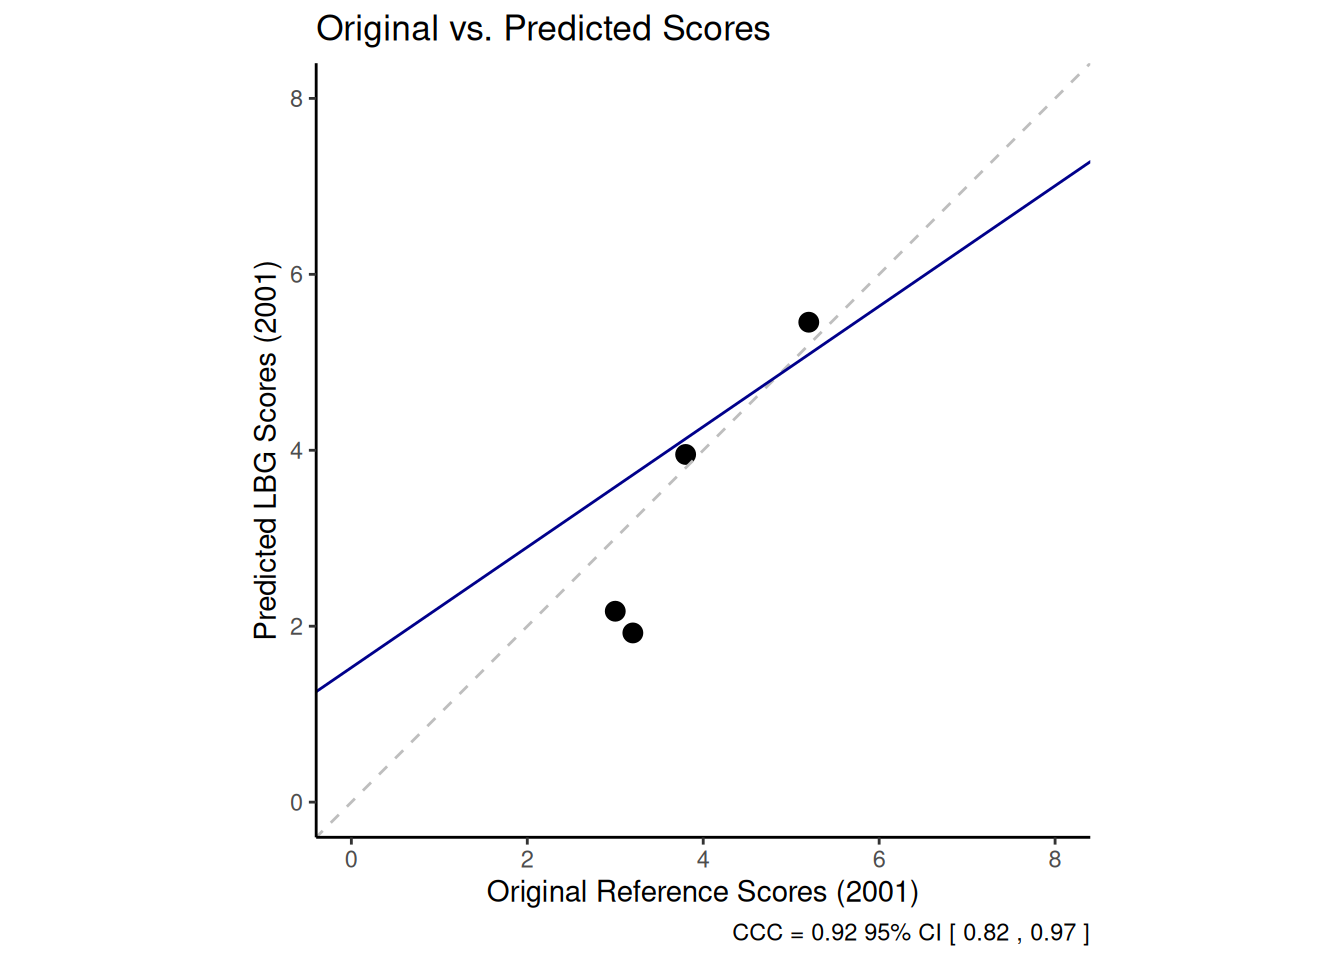
\includegraphics[keepaspectratio]{Introduction-to-Quantitative-Text-Analysis_files/figure-latex/ggplot-wordscores-ccc-1.pdf}}

This graph enables us to inspect the level of agreement visually. Points close to the dashed 45-degree line suggest accurate predictions. Deviations from this line show areas where the model struggles to reproduce the original values. Identifying points far from the line (outliers) can help us to diagnose problems, such as a particular reference text whose language does not align well with its assigned score compared to the other texts.

As well as positioning the texts, we can look at the word scores themselves. Plotting word scores can show which words are most strongly associated with different positions on the scale. The \texttt{textplot\_scale1d()} function from \texttt{quanteda.textplots} is useful. We specify \texttt{margin\ =\ "features"} to plot the word scores and can highlight specific words of interest.

\begin{Shaded}
\begin{Highlighting}[]
\FunctionTok{library}\NormalTok{(quanteda.textplots)}

\CommentTok{\# Plot the distribution of word scores}
\FunctionTok{textplot\_scale1d}\NormalTok{(ws, }\AttributeTok{margin =} \StringTok{"features"}\NormalTok{, }\AttributeTok{highlighted =} \FunctionTok{c}\NormalTok{(}\StringTok{"british"}\NormalTok{, }\StringTok{"vote"}\NormalTok{, }\StringTok{"europe"}\NormalTok{,}
    \StringTok{"taxes"}\NormalTok{, }\StringTok{"economy"}\NormalTok{, }\StringTok{"immigration"}\NormalTok{)  }\CommentTok{\# Highlight relevant words on the plot}
\NormalTok{)}
\end{Highlighting}
\end{Shaded}

\pandocbounded{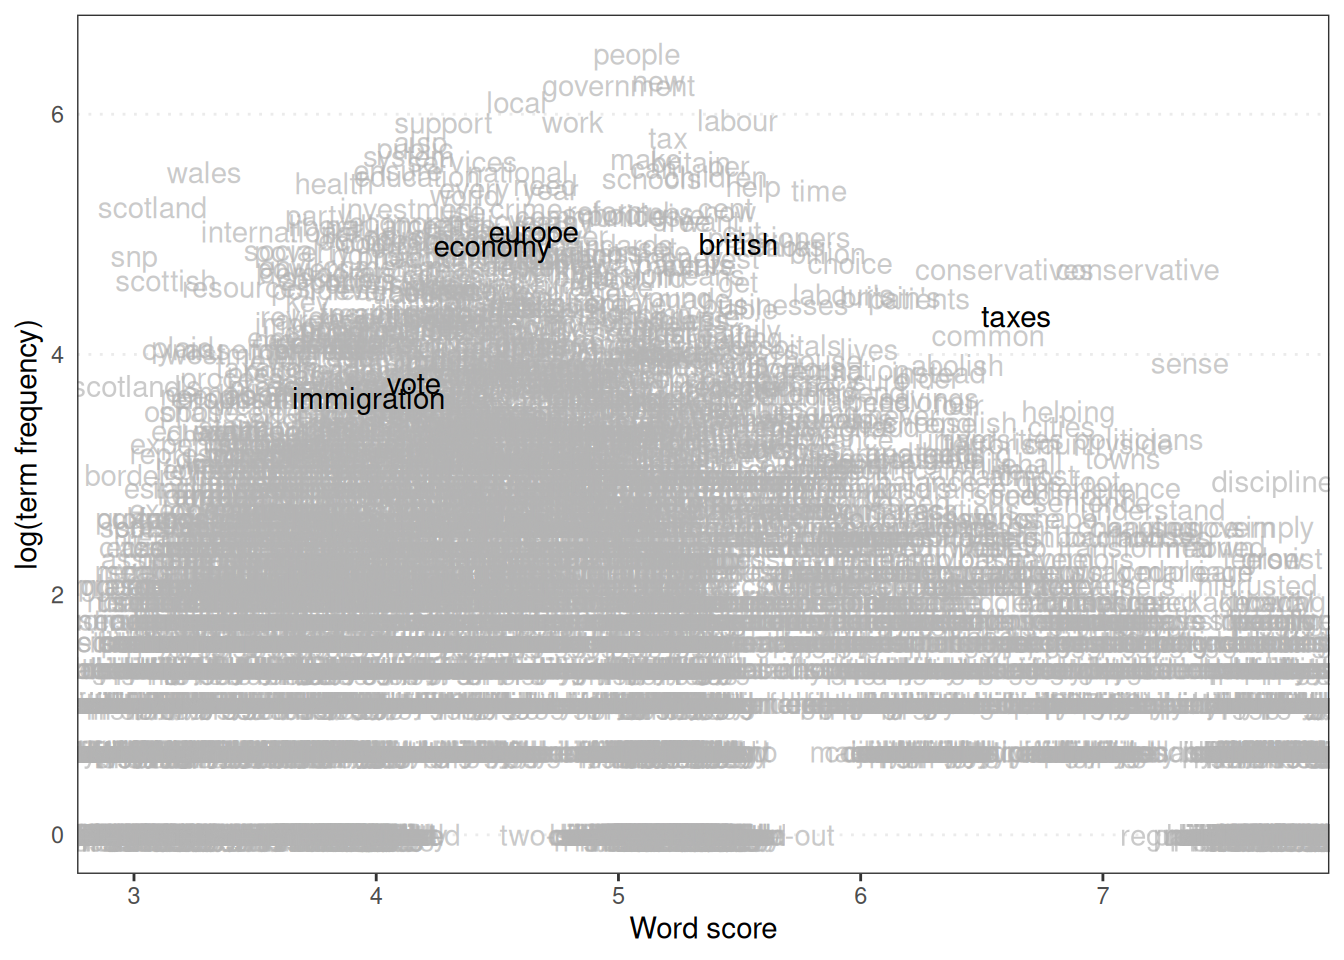
\includegraphics[keepaspectratio]{Introduction-to-Quantitative-Text-Analysis_files/figure-latex/wordscores-textplotscale-features-1.pdf}}

The position of words on the scale indicates their estimated ideological leaning based on the reference texts. Words like `taxes' or `economy' might be expected to fall towards one end (e.g.~left). In contrast, words related to national identity or immigration might be closer to the other (e.g.~right), depending on the corpus and the reference scores.

Finally, we can examine the confidence intervals around the estimated text scores, which is particularly important for the virgin texts, as it measures the uncertainty in their estimated positions. The \texttt{textplot\_scale1d()} function can also plot document scores with confidence intervals when \texttt{margin\ =\ "documents"} is specified, but this requires the standard errors to be available, which is the case for the MV rescaling method (\texttt{pred\_mv}):

\begin{Shaded}
\begin{Highlighting}[]
\FunctionTok{textplot\_scale1d}\NormalTok{(pred\_mv, }\AttributeTok{margin =} \StringTok{"documents"}  \CommentTok{\# Specify that we want to plot document scores}
\NormalTok{)}
\end{Highlighting}
\end{Shaded}

\pandocbounded{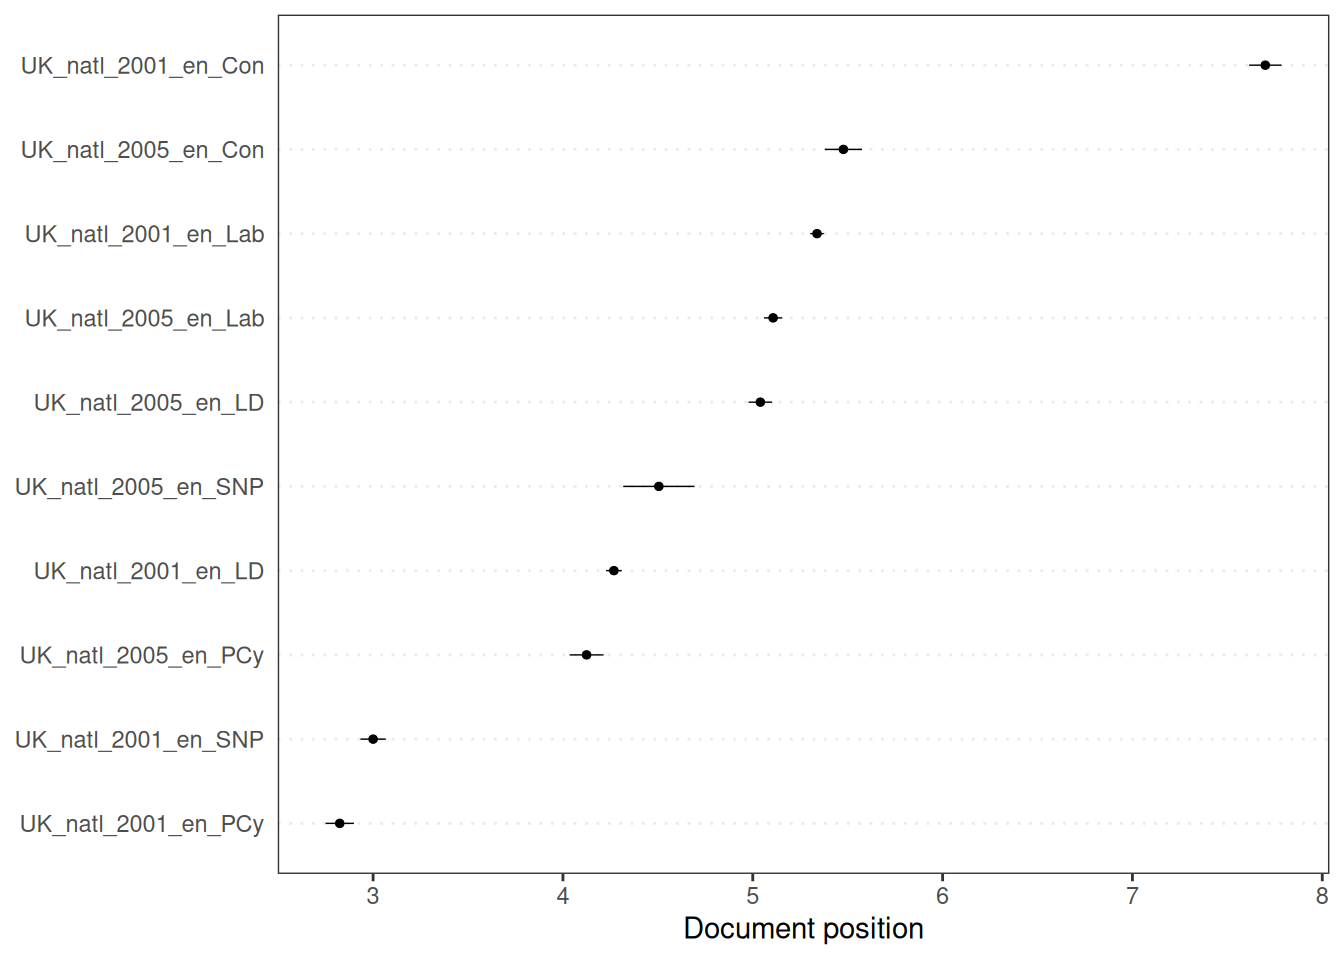
\includegraphics[keepaspectratio]{Introduction-to-Quantitative-Text-Analysis_files/figure-latex/wordscores-textplotscale-documents-1.pdf}}

The length of the error bars in this graph indicates the width of the confidence interval. Longer error bars indicate greater uncertainty in the estimated position of the document in question. This uncertainty may be due to various factors, such as the number of dictionary words in the document, variability in the scores of these words and the quantity and quality of the reference texts. We can manually create this document scaling plot using \texttt{ggplot2} and the results from \texttt{pred\_mv}. This requires manipulating the data to extract the scores and confidence intervals and document information into a data frame, for which we can use the \texttt{dplyr} package:

\begin{Shaded}
\begin{Highlighting}[]
\FunctionTok{library}\NormalTok{(dplyr)}
\FunctionTok{library}\NormalTok{(stringr)}
\FunctionTok{library}\NormalTok{(tibble)}

\CommentTok{\# Extract predicted fit and standard error}

\NormalTok{scores\_fit }\OtherTok{\textless{}{-}} \FunctionTok{as.data.frame}\NormalTok{(pred\_mv}\SpecialCharTok{$}\NormalTok{fit) }\SpecialCharTok{\%\textgreater{}\%}
  \FunctionTok{rename}\NormalTok{(}\AttributeTok{fit =} \DecValTok{1}\NormalTok{) }\CommentTok{\# Rename the column to \textquotesingle{}fit\textquotesingle{}}

\NormalTok{scores\_se }\OtherTok{\textless{}{-}} \FunctionTok{as.data.frame}\NormalTok{(pred\_mv}\SpecialCharTok{$}\NormalTok{se.fit) }\SpecialCharTok{\%\textgreater{}\%}
  \FunctionTok{rename}\NormalTok{(}\AttributeTok{se =} \DecValTok{1}\NormalTok{) }\CommentTok{\# Rename the column to \textquotesingle{}se\textquotesingle{}}

\CommentTok{\# Combine fit and SE data frames and add document metadata}

\NormalTok{data\_textplot }\OtherTok{\textless{}{-}}\NormalTok{ scores\_fit }\SpecialCharTok{\%\textgreater{}\%}
  \FunctionTok{bind\_cols}\NormalTok{(scores\_se) }\SpecialCharTok{\%\textgreater{}\%} \CommentTok{\# Combine the \textquotesingle{}fit\textquotesingle{} and \textquotesingle{}se\textquotesingle{} data frames side by side}
  \FunctionTok{rownames\_to\_column}\NormalTok{(}\StringTok{"doc\_id"}\NormalTok{) }\SpecialCharTok{\%\textgreater{}\%} \CommentTok{\# Convert the row names (which are the document IDs) into a new column named \textquotesingle{}doc\_id\textquotesingle{}}
  \FunctionTok{mutate}\NormalTok{(}
    \AttributeTok{lwr =}\NormalTok{ fit }\SpecialCharTok{{-}} \FloatTok{1.96} \SpecialCharTok{*}\NormalTok{ se,}
    \CommentTok{\# Calculate the lower bound of the 95\% confidence interval (assuming normal distribution)}
    \AttributeTok{upr =}\NormalTok{ fit }\SpecialCharTok{+} \FloatTok{1.96} \SpecialCharTok{*}\NormalTok{ se,}
    \CommentTok{\# Calculate the upper bound of the 95\% confidence interval}
    \AttributeTok{year =} \FunctionTok{factor}\NormalTok{(}\FunctionTok{str\_extract}\NormalTok{(doc\_id, }\StringTok{"}\SpecialCharTok{\textbackslash{}\textbackslash{}}\StringTok{d\{4\}"}\NormalTok{)),}
    \CommentTok{\# Extract the year (four digits) from the doc\_id and convert to a factor}
    \AttributeTok{party =} \FunctionTok{str\_replace}\NormalTok{(doc\_id, }\StringTok{"}\SpecialCharTok{\textbackslash{}\textbackslash{}}\StringTok{d\{4\}\_"}\NormalTok{, }\StringTok{""}\NormalTok{),}
    \CommentTok{\# Remove the year and underscore from the doc\_id to get the party name}
    \AttributeTok{label =} \FunctionTok{factor}\NormalTok{(}\FunctionTok{paste}\NormalTok{(party, year), }\AttributeTok{levels =} \FunctionTok{paste}\NormalTok{(party, year)[}\FunctionTok{order}\NormalTok{(fit)]) }\CommentTok{\# Create a combined label of party and year, ordered by the \textquotesingle{}fit\textquotesingle{} score for plotting}
\NormalTok{  ) }\SpecialCharTok{\%\textgreater{}\%}
  \FunctionTok{select}\NormalTok{(doc\_id, fit, lwr, upr, se, year, party, label) }\CommentTok{\# Select and reorder the columns}

\FunctionTok{head}\NormalTok{(data\_textplot)}
\end{Highlighting}
\end{Shaded}

\begin{verbatim}
##                doc_id      fit      lwr      upr         se year          party
## 1 UK_natl_2001_en_Con 7.700000 7.614306 7.785694 0.04372127 2001 UK_natl_en_Con
## 2 UK_natl_2001_en_Lab 5.338408 5.302650 5.374166 0.01824402 2001 UK_natl_en_Lab
## 3  UK_natl_2001_en_LD 4.268507 4.227169 4.309846 0.02109101 2001  UK_natl_en_LD
## 4 UK_natl_2001_en_PCy 2.824328 2.749560 2.899097 0.03814726 2001 UK_natl_en_PCy
## 5 UK_natl_2001_en_SNP 3.000000 2.933106 3.066894 0.03412945 2001 UK_natl_en_SNP
## 6 UK_natl_2005_en_Con 5.477515 5.379665 5.575364 0.04992337 2005 UK_natl_en_Con
##                 label
## 1 UK_natl_en_Con 2001
## 2 UK_natl_en_Lab 2001
## 3  UK_natl_en_LD 2001
## 4 UK_natl_en_PCy 2001
## 5 UK_natl_en_SNP 2001
## 6 UK_natl_en_Con 2005
\end{verbatim}

Now that we have the data in a convenient format, we can plot the estimated document positions with their confidence intervals using \texttt{ggplot2}. Ordering the documents by their estimated score on the y-axis is often helpful for visualisation.

\begin{Shaded}
\begin{Highlighting}[]
\FunctionTok{library}\NormalTok{(ggplot2)}

\FunctionTok{ggplot}\NormalTok{(data\_textplot, }\FunctionTok{aes}\NormalTok{(}\AttributeTok{x =}\NormalTok{ fit, }\AttributeTok{y =}\NormalTok{ label, }\AttributeTok{colour =}\NormalTok{ year)) }\SpecialCharTok{+}
  \FunctionTok{geom\_point}\NormalTok{(}\AttributeTok{size =} \DecValTok{3}\NormalTok{) }\SpecialCharTok{+}
  \FunctionTok{scale\_x\_continuous}\NormalTok{(}\AttributeTok{name =} \StringTok{"Left {-} Right Score"}\NormalTok{) }\SpecialCharTok{+}
  \FunctionTok{geom\_errorbarh}\NormalTok{(}\FunctionTok{aes}\NormalTok{(}\AttributeTok{xmax =}\NormalTok{ upr, }\AttributeTok{xmin =}\NormalTok{ lwr),}
                 \AttributeTok{height =} \DecValTok{0}\NormalTok{,}
                 \AttributeTok{linewidth =} \FloatTok{0.8}\NormalTok{) }\SpecialCharTok{+}
  \FunctionTok{theme\_classic}\NormalTok{() }\SpecialCharTok{+}
  \FunctionTok{scale\_colour\_manual}\NormalTok{(}
    \AttributeTok{values =} \FunctionTok{c}\NormalTok{(}\StringTok{"2001"} \OtherTok{=} \StringTok{"\#ffa600"}\NormalTok{, }\StringTok{"2005"} \OtherTok{=} \StringTok{"\#ff6361"}\NormalTok{),}
    \CommentTok{\# Define custom colours for the years 2001 and 2005}
    \AttributeTok{name =} \StringTok{"Years"}
\NormalTok{  ) }\SpecialCharTok{+} \CommentTok{\# Set the title for the colour legend}
  \FunctionTok{ggtitle}\NormalTok{(}\StringTok{"Left{-}Right Distribution of UK Party Manifestos (Wordscores MV)"}\NormalTok{,}
          \AttributeTok{subtitle =} \StringTok{"with 95\% confidence intervals"}\NormalTok{) }\SpecialCharTok{+}
  \FunctionTok{theme}\NormalTok{(}
    \AttributeTok{plot.title =} \FunctionTok{element\_text}\NormalTok{(}\AttributeTok{size =} \DecValTok{14}\NormalTok{, }\AttributeTok{hjust =} \FloatTok{0.5}\NormalTok{),}
    \AttributeTok{plot.subtitle =} \FunctionTok{element\_text}\NormalTok{(}\AttributeTok{hjust =} \FloatTok{0.5}\NormalTok{),}
    \AttributeTok{legend.position =} \StringTok{"top"}\NormalTok{,}
    \AttributeTok{axis.title.y =} \FunctionTok{element\_blank}\NormalTok{()}
\NormalTok{  )}
\end{Highlighting}
\end{Shaded}

\pandocbounded{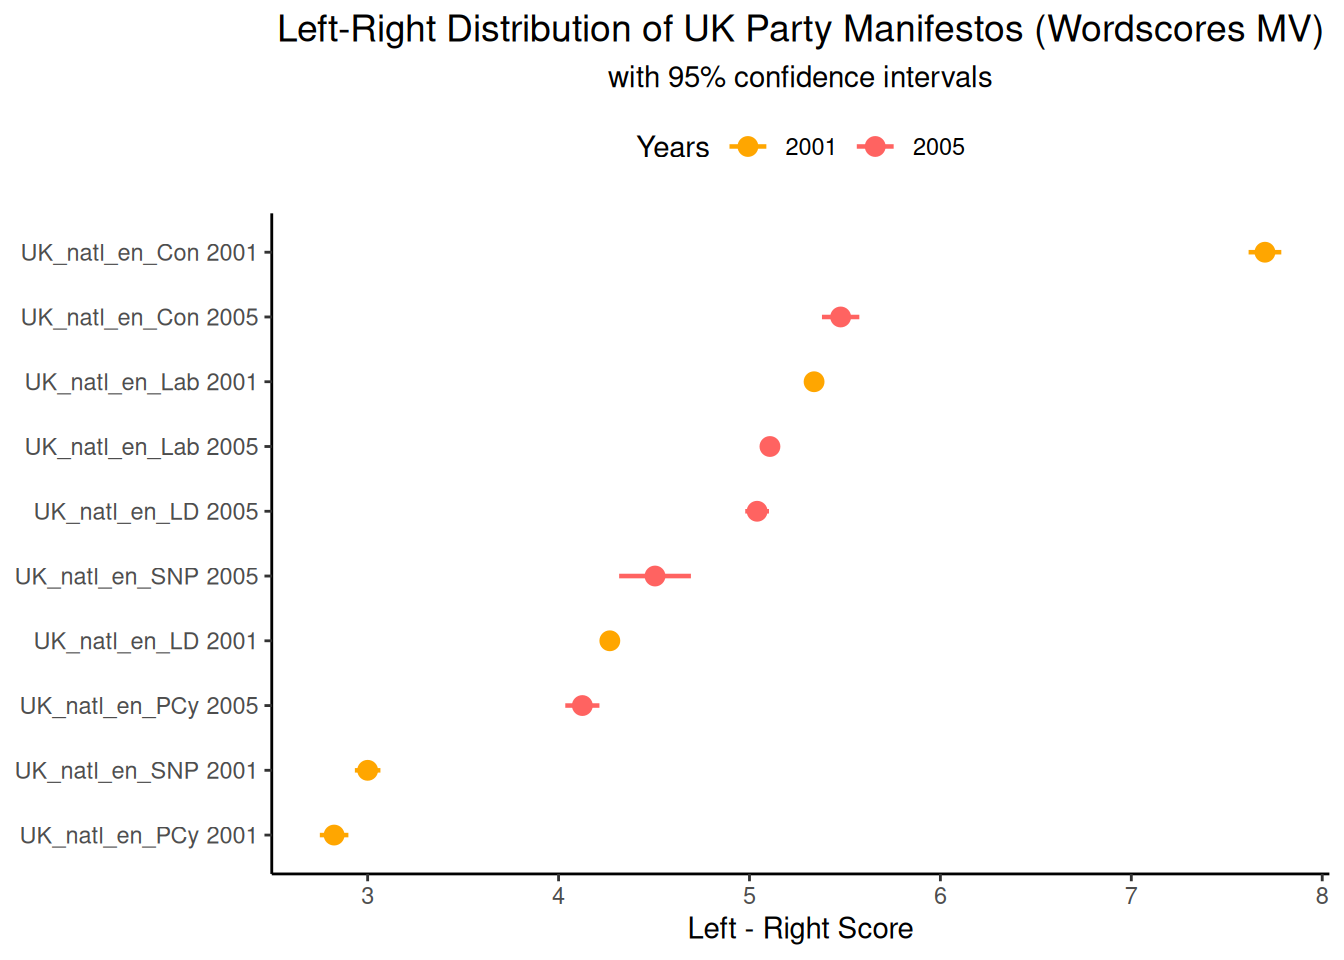
\includegraphics[keepaspectratio]{Introduction-to-Quantitative-Text-Analysis_files/figure-latex/ggplot-wordscores-textplotscale-1.pdf}}

This graph shows the estimated left-right position of each manifesto in 2001 and 2005, as well as the uncertainty of the 2005 estimates. It shows the parties' relative positions and how their estimated values may have changed between the two election years. The width of the confidence intervals indicates which estimates are less specific, potentially because of limited text length or vocabulary overlap with the reference texts.

\section{Wordfish}\label{wordfish}

Unlike Wordscores, Wordfish is an unsupervised scaling method. It does not require pre-scored reference texts. Instead, it models word frequencies in documents based on a Poisson distribution while simultaneously estimating document positions and word-specific parameters. The model assumes that a word's frequency in a document is related to the document's position on a single latent dimension, the word's overall tendency to occur in the document, and its specific association with the latent dimension.

The output of Wordfish includes
* \(\theta\) (theta): The estimated position of each document on the latent dimension.
* \(\alpha\) (alpha): The estimated intercept for each word, representing its overall frequency.
* \(\beta\) (beta): The estimated weight for each word, representing its association with the latent dimension. Words with large positive beta values are more likely to appear in documents with high theta values, and vice versa for large negative beta values.
* \(\psi\) (psi): A document-specific fixed effect that captures variations in document length.

Wordfish estimates a single latent dimension. The direction of this dimension is arbitrary (e.g.~left to right or right to left). We can orient the dimension by specifying two \emph{anchor texts} or by selecting a direction using the \texttt{dir} argument in \texttt{textmodel\_wordfish()}.

Let's apply Wordfish to a corpus of US presidential inaugural speeches. We will use speeches after 1900 and preprocess the texts similarly to the Wordscores example. We could choose speeches from presidents typically considered at opposite ends of a relevant dimension (such as a left-right scale) to orient the scale. For example, we could use the 1965 Johnson and the 1985 Reagan speeches to define the direction, arbitrarily assigning one speech to one end of the scale and the other to the other.

\begin{Shaded}
\begin{Highlighting}[]
\FunctionTok{library}\NormalTok{(quanteda)}
\FunctionTok{data}\NormalTok{(data\_corpus\_inaugural)}
\FunctionTok{set.seed}\NormalTok{(}\DecValTok{42}\NormalTok{)}

\NormalTok{corpus\_inaugural }\OtherTok{\textless{}{-}} \FunctionTok{corpus\_subset}\NormalTok{(data\_corpus\_inaugural, Year }\SpecialCharTok{\textgreater{}} \DecValTok{1900}\NormalTok{)}

\CommentTok{\# Tokenise and preprocess the corpus}
\NormalTok{data\_inaugural\_tokens }\OtherTok{\textless{}{-}} \FunctionTok{tokens}\NormalTok{(}
\NormalTok{ corpus\_inaugural,}
 \AttributeTok{what =} \StringTok{"word"}\NormalTok{,}
 \AttributeTok{remove\_punct =} \ConstantTok{TRUE}\NormalTok{, }\CommentTok{\# Remove punctuation}
 \AttributeTok{remove\_symbols =} \ConstantTok{TRUE}\NormalTok{, }\CommentTok{\# Remove symbols}
 \AttributeTok{remove\_numbers =} \ConstantTok{TRUE}\NormalTok{, }\CommentTok{\# Remove numbers}
 \AttributeTok{remove\_url =} \ConstantTok{TRUE}\NormalTok{, }\CommentTok{\# Remove URLs}
 \AttributeTok{remove\_separators =} \ConstantTok{TRUE}\NormalTok{, }\CommentTok{\# Remove separators}
 \AttributeTok{split\_hyphens =} \ConstantTok{FALSE}\NormalTok{, }\CommentTok{\# Do not split hyphenated words}
 \AttributeTok{include\_docvars =} \ConstantTok{TRUE} \CommentTok{\# Include document variables (metadata)}
\NormalTok{)}

\NormalTok{data\_inaugural\_tokens }\OtherTok{\textless{}{-}} \FunctionTok{tokens\_tolower}\NormalTok{(data\_inaugural\_tokens) }
\NormalTok{data\_inaugural\_tokens }\OtherTok{\textless{}{-}} \FunctionTok{tokens\_select}\NormalTok{(data\_inaugural\_tokens, }\FunctionTok{stopwords}\NormalTok{(}\StringTok{"english"}\NormalTok{), }\AttributeTok{selection =} \StringTok{"remove"}\NormalTok{)}

\NormalTok{data\_inaugural\_dfm }\OtherTok{\textless{}{-}} \FunctionTok{dfm}\NormalTok{(data\_inaugural\_tokens)}

\CommentTok{\# Print document names to identify indices for direction. We needed the order of documents to specify anchor texts by index}
\NormalTok{data\_inaugural\_dfm}\SpecialCharTok{@}\NormalTok{Dimnames}\SpecialCharTok{$}\NormalTok{docs}
\end{Highlighting}
\end{Shaded}

\begin{verbatim}
##  [1] "1901-McKinley"   "1905-Roosevelt"  "1909-Taft"       "1913-Wilson"    
##  [5] "1917-Wilson"     "1921-Harding"    "1925-Coolidge"   "1929-Hoover"    
##  [9] "1933-Roosevelt"  "1937-Roosevelt"  "1941-Roosevelt"  "1945-Roosevelt" 
## [13] "1949-Truman"     "1953-Eisenhower" "1957-Eisenhower" "1961-Kennedy"   
## [17] "1965-Johnson"    "1969-Nixon"      "1973-Nixon"      "1977-Carter"    
## [21] "1981-Reagan"     "1985-Reagan"     "1989-Bush"       "1993-Clinton"   
## [25] "1997-Clinton"    "2001-Bush"       "2005-Bush"       "2009-Obama"     
## [29] "2013-Obama"      "2017-Trump"      "2025-Trump"      "2021-Biden.txt"
\end{verbatim}

\begin{Shaded}
\begin{Highlighting}[]
\CommentTok{\# Identify the indices of the anchor documents (1965 Johnson and 1985 Reagan)}
\NormalTok{johnson\_index }\OtherTok{\textless{}{-}} \FunctionTok{which}\NormalTok{(}\FunctionTok{docnames}\NormalTok{(data\_inaugural\_dfm) }\SpecialCharTok{==} \StringTok{"1965{-}Johnson"}\NormalTok{)}
\NormalTok{reagan\_index }\OtherTok{\textless{}{-}} \FunctionTok{which}\NormalTok{(}\FunctionTok{docnames}\NormalTok{(data\_inaugural\_dfm) }\SpecialCharTok{==} \StringTok{"1985{-}Reagan"}\NormalTok{)}

\NormalTok{wordfish }\OtherTok{\textless{}{-}} \FunctionTok{textmodel\_wordfish}\NormalTok{(data\_inaugural\_dfm, }\AttributeTok{dir =} \FunctionTok{c}\NormalTok{(johnson\_index, reagan\_index))}
\FunctionTok{summary}\NormalTok{(wordfish)}
\end{Highlighting}
\end{Shaded}

\begin{verbatim}
## 
## Call:
## textmodel_wordfish.dfm(x = data_inaugural_dfm, dir = c(johnson_index, 
##     reagan_index))
## 
## Estimated Document Positions:
##                   theta      se
## 1901-McKinley    1.5231 0.03445
## 1905-Roosevelt   0.5721 0.07408
## 1909-Taft        2.1237 0.01546
## 1913-Wilson      0.9976 0.04989
## 1917-Wilson      0.8953 0.05631
## 1921-Harding     1.3240 0.03016
## 1925-Coolidge    1.4477 0.02699
## 1929-Hoover      1.5517 0.02676
## 1933-Roosevelt   1.1239 0.04450
## 1937-Roosevelt   0.6780 0.05084
## 1941-Roosevelt   0.1642 0.06566
## 1945-Roosevelt  -0.1975 0.10062
## 1949-Truman      0.8955 0.04309
## 1953-Eisenhower  0.3971 0.04596
## 1957-Eisenhower  0.2409 0.05696
## 1961-Kennedy    -0.4300 0.05878
## 1965-Johnson    -0.7405 0.05306
## 1969-Nixon      -0.8995 0.03988
## 1973-Nixon      -0.4312 0.05319
## 1977-Carter     -0.2595 0.06574
## 1981-Reagan     -0.6129 0.04347
## 1985-Reagan     -0.6120 0.04098
## 1989-Bush       -0.8492 0.03989
## 1993-Clinton    -0.9815 0.04284
## 1997-Clinton    -0.8017 0.04026
## 2001-Bush       -0.7856 0.04875
## 2005-Bush       -0.4165 0.04827
## 2009-Obama      -0.9093 0.03711
## 2013-Obama      -0.9255 0.03917
## 2017-Trump      -1.1277 0.04045
## 2025-Trump      -1.4772 0.02322
## 2021-Biden.txt  -1.4772 0.02322
## 
## Estimated Feature Scores:
##      fellow-citizens assembled    4th    march    great anxiety  regard
## beta           2.139   -0.0889  1.345  0.02153 -0.07759  0.6057  0.9199
## psi           -4.906   -2.8417 -4.789 -1.77253  1.51900 -2.8294 -2.3046
##      currency  credit    none  exists     now treasury receipts inadequate
## beta    2.167  0.9628  0.5128 -0.5351 -0.4631    1.528    2.346     0.2772
## psi    -3.972 -2.2206 -2.2387 -2.4414  1.2856   -4.357   -5.658    -2.2953
##         meet current obligations government sufficient   public   needs surplus
## beta -0.4061   1.534      0.4229     0.2488     0.6309  0.42348 -0.1739   1.345
## psi   0.1697  -3.672     -0.9451     1.6480    -1.4662 -0.04104 -0.8127  -4.789
##      instead  deficit    felt constrained convene congress extraordinary
## beta -1.0077 -0.02742  0.4259       1.345   1.345   0.7940        0.7832
## psi  -0.8927 -1.47020 -2.3942      -4.789  -4.789  -0.3057       -3.0024
\end{verbatim}

The \texttt{summary()} output for a Wordfish model provides information about the model fit and the estimated parameters (\(\theta\), \(\alpha\), \(\beta\), \(\psi\)). The \(\theta\) values are the estimated positions of the documents on the latent dimension. Like Wordscores, we can use the \texttt{predict()} function to obtain the estimated document positions with confidence intervals. The estimated position (\texttt{theta}) is called the \texttt{fit} in the output.

\begin{Shaded}
\begin{Highlighting}[]
\NormalTok{pred\_wordfish }\OtherTok{\textless{}{-}} \FunctionTok{predict}\NormalTok{(wordfish, }\AttributeTok{interval =} \StringTok{"confidence"}\NormalTok{)}
\end{Highlighting}
\end{Shaded}

Using the \texttt{textplot\_scale1d()} function, similar to Wordscores, we can visualise the estimated document positions and the word parameters. Plotting the word parameters (\texttt{margin\ =\ "features"}) shows which words are associated with which end of the latent dimension.

\begin{Shaded}
\begin{Highlighting}[]
\FunctionTok{library}\NormalTok{(quanteda.textplots)}
\FunctionTok{textplot\_scale1d}\NormalTok{(wordfish,}
                 \AttributeTok{margin =} \StringTok{"features"}\NormalTok{, }\CommentTok{\# Plot features (words)}
                 \AttributeTok{highlighted =} \FunctionTok{c}\NormalTok{(}\StringTok{"america"}\NormalTok{, }\StringTok{"great"}\NormalTok{, }\StringTok{"freedom"}\NormalTok{, }\StringTok{"government"}\NormalTok{, }\StringTok{"taxes"}\NormalTok{, }\StringTok{"people"}\NormalTok{, }\StringTok{"world"}\NormalTok{)}
\NormalTok{                 )}
\end{Highlighting}
\end{Shaded}

\pandocbounded{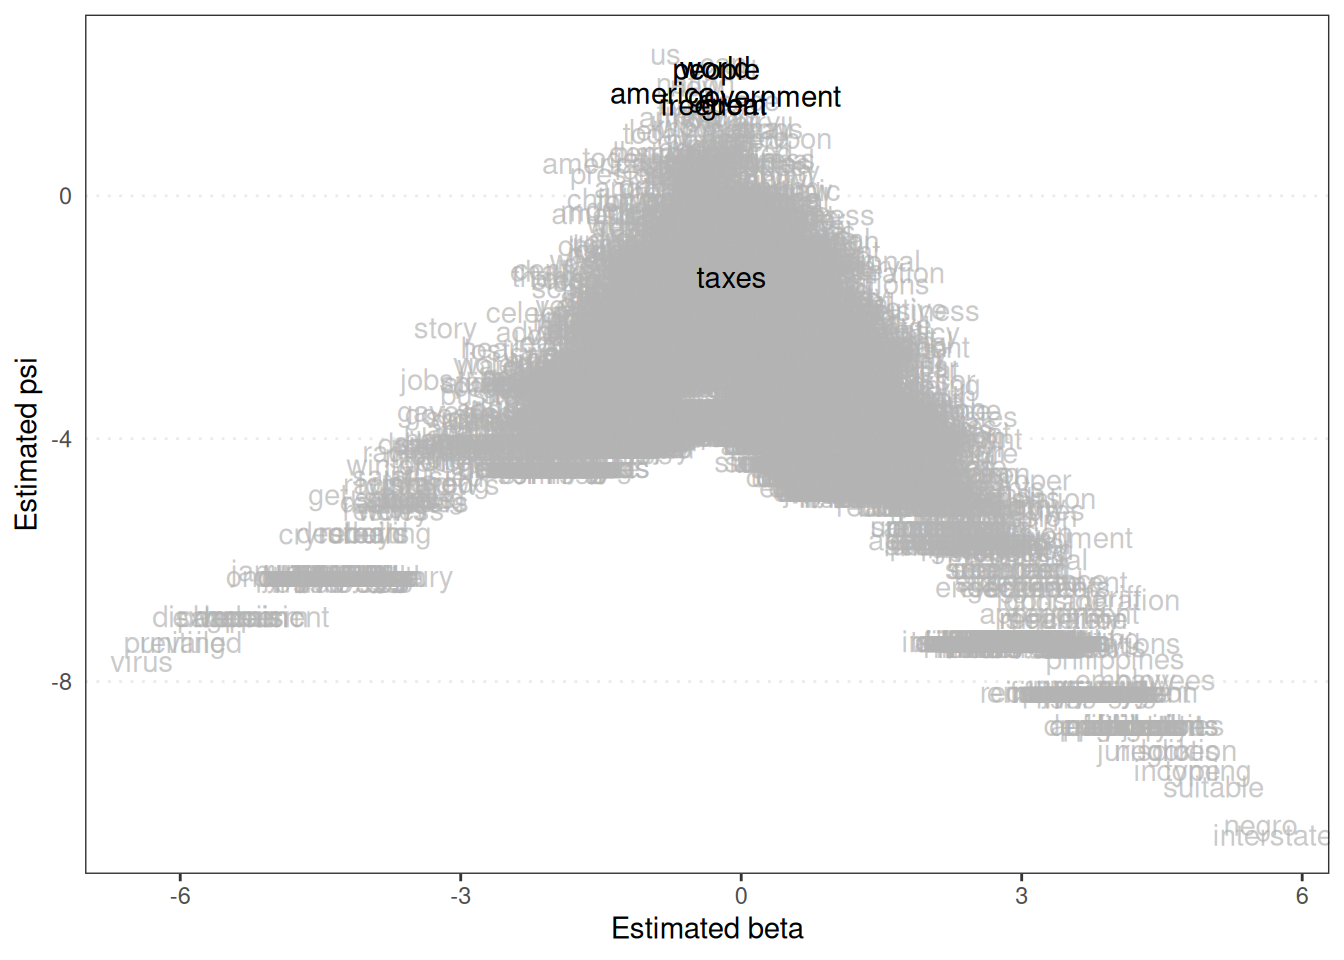
\includegraphics[keepaspectratio]{Introduction-to-Quantitative-Text-Analysis_files/figure-latex/wordfish-textplot-features-1.pdf}}

A word's position on this scale corresponds to its \(\beta\) value. Words at one end of the scale are more likely to appear in documents with high \(\theta\) values, and words at the other extreme are more likely to appear in documents with low \(\theta\) values. How we interpret the scale depends on the words we find at the extremes and any anchor texts used for orientation. Plotting document positions (\texttt{margin\ =\ "documents"} ) visualises the estimated values of \(\theta\).

\begin{Shaded}
\begin{Highlighting}[]
\CommentTok{\# Plot the distribution of document positions (theta values) with confidence}
\CommentTok{\# intervals. Theta values are the estimated document scores on the latent}
\CommentTok{\# dimension.}
\FunctionTok{textplot\_scale1d}\NormalTok{(wordfish, }\AttributeTok{margin =} \StringTok{"documents"}  \CommentTok{\# Plot documents}
\NormalTok{)}
\end{Highlighting}
\end{Shaded}

\pandocbounded{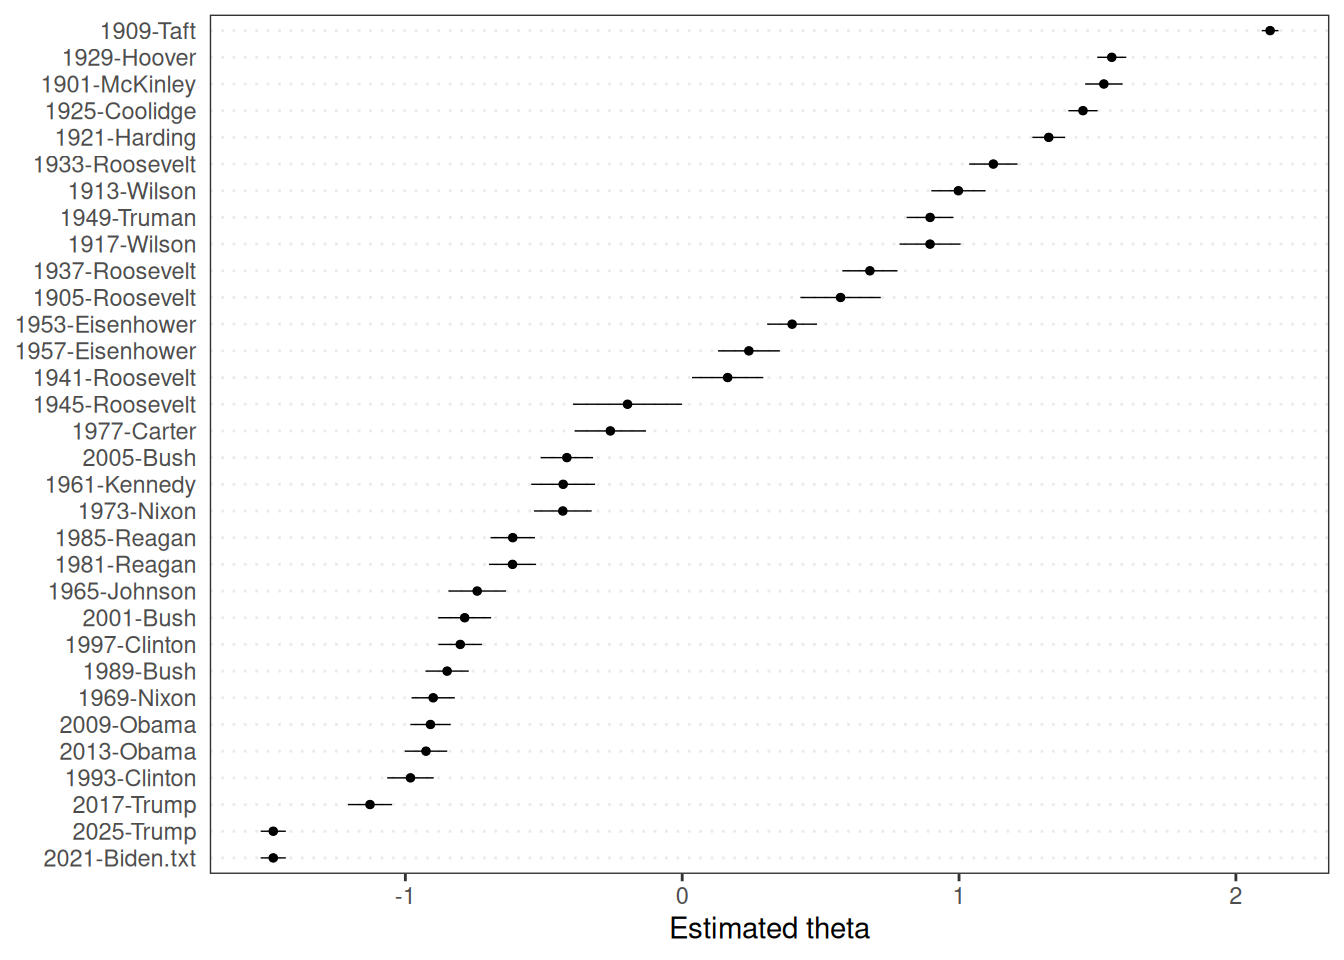
\includegraphics[keepaspectratio]{Introduction-to-Quantitative-Text-Analysis_files/figure-latex/wordfish-textplot-documents-1.pdf}}

This graph shows the estimated position of each inaugural address on the latent dimension, ordered by year. The confidence intervals indicate the uncertainty of these estimates. Interpreting this dimension requires careful consideration of the anchor texts used and the words that load highly on the dimension (from the word plot). For example, suppose we anchor with a president who is typically considered `liberal' at one end and `conservative' at the other, and the word plot shows terms related to social programmes at one end and terms related to individual freedom at the other. In that case, we might interpret this as a left-right political dimension. However, Wordfish can uncover any dominant latent dimension in the text, which may not always conform to preconceived notions such as a simple left-right scale.

Wordfish is a valuable tool for discovering latent dimensions in text data without relying on external scores. Its unsupervised nature can be both a strength (no need for reference data) and a weakness (latent dimension interpretation is not always straightforward and requires careful analysis of word loadings).

\section{Correspondence Analysis}\label{correspondence-analysis}

Correspondence analysis (CA) is a dimensionality reduction technique used to analyse the relationship between categorical variables. In text analysis, it is often applied to document feature matrices (DFM) to explore the associations between documents and words. CA can be considered categorical data (or count data treated as frequencies or proportions) equivalent to Principal Component Analysis (PCA). It simultaneously positions documents and features (words) in a low-dimensional space, where proximity between points indicates association.

\begin{itemize}
\tightlist
\item
  \textbf{Simple Correspondence Analysis (SCA)} is applied to a two-way contingency table (like a dfm).
\item
  \textbf{Multiple Correspondence Analysis (MCA)} is an extension used to analyse relationships between more than two categorical variables and is often applied to surveys or questionnaires. While a DFM is inherently a two-way table, MCA can be used by treating the presence or absence of each word in a document as a categorical variable. However, this approach is less common than applying SCA directly to the dfm or using specialised text analysis functions that perform a form of CA.
\end{itemize}

Here, we look at an example using a dataset where the text has been coded into specific categories, making it suitable for MCA. The example uses data from an article on the stylistic variation in Donald Trump's Twitter data (which we already looked at earlier) between 2009 and 2018 (\citeproc{ref-Clarke2019a}{Clarke \& Grieve, 2019}). In this study, the authors downloaded 21,739 tweets and grouped them into 63 categories over 5 dimensions based on their content. First, we load the packages we need for the Correspondence Analysis:

Although there is a CA function in \texttt{quanteda}, here, we first look at \texttt{FactoMineR} and \texttt{factoextra}, which allow us several interesting possibilities. \texttt{FactoMineR} is renowned for its extensive range of exploratory data analysis functions, including CA and MCA, and it integrates seamlessly with \texttt{factoextra} for visualisation. First, we load the necessary packages and the dataset:

\begin{Shaded}
\begin{Highlighting}[]
\FunctionTok{library}\NormalTok{(FactoMineR)}
\FunctionTok{library}\NormalTok{(factoextra)}
\FunctionTok{library}\NormalTok{(readr)}
\FunctionTok{library}\NormalTok{(dplyr)}
\end{Highlighting}
\end{Shaded}

Then, we import the data, which should contain categorised information about the tweets. As before, you can load the data directly from the URL:

\begin{Shaded}
\begin{Highlighting}[]
\NormalTok{urlfile }\OtherTok{=} \StringTok{"https://raw.githubusercontent.com/SCJBruinsma/qta{-}files/master/TRUMP\_DATA.csv"}
\NormalTok{tweets }\OtherTok{\textless{}{-}} \FunctionTok{read\_csv}\NormalTok{(}\FunctionTok{url}\NormalTok{(urlfile), }\AttributeTok{show\_col\_types =} \ConstantTok{FALSE}\NormalTok{)}
\FunctionTok{head}\NormalTok{(tweets)}
\end{Highlighting}
\end{Shaded}

This dataset contains several variables, including categorisations of the tweets and possibly other metadata. For the MCA, we must select the columns representing the categorical variables we want to analyse (the 63 categories mentioned in the original text). We will also sample a subset of the tweets for faster processing.

\begin{Shaded}
\begin{Highlighting}[]
\NormalTok{tweets }\OtherTok{\textless{}{-}}\NormalTok{ tweets[}\FunctionTok{sample}\NormalTok{(}\FunctionTok{nrow}\NormalTok{(tweets), }\DecValTok{500}\NormalTok{), ]}
\NormalTok{tweets\_mat }\OtherTok{\textless{}{-}}\NormalTok{ tweets[, }\DecValTok{2}\SpecialCharTok{:}\DecValTok{65}\NormalTok{]  }\CommentTok{\# Select columns 2 through 65, which contain the categorical variables for MCA.}
\end{Highlighting}
\end{Shaded}

We can then run the Multiple Correspondence Analysis using the \texttt{MCA()} function from the \texttt{FactoMineR} package. When we provide the data frame containing the categorical variables, we need to specify the number of dimensions (\texttt{ncp}) to retain. We can determine this by examining the eigenvalues (similar to a scree plot in PCA) or base ourselves on theoretical considerations. Here, we use 5, as this was the number of dimensions found by Clarke \& Grieve (\citeproc{ref-Clarke2019a}{2019}). In addition, we can include supplementary quantitative variables (\texttt{quanti.sup}) or supplementary individuals (\texttt{ind.sup}) that do not contribute to the MCA but are projected onto the resulting dimensions. Here, we include `Tweet.Length' as a supplementary quantitative variable:

\begin{Shaded}
\begin{Highlighting}[]
\NormalTok{mca\_tweets }\OtherTok{\textless{}{-}} \FunctionTok{MCA}\NormalTok{(tweets\_mat, }\AttributeTok{ncp =} \DecValTok{5}\NormalTok{, }\AttributeTok{quanti.sup =} \DecValTok{1}\NormalTok{, }\AttributeTok{graph =} \ConstantTok{FALSE}\NormalTok{)  }\CommentTok{\# \textquotesingle{}ncp=5\textquotesingle{} specifies keeping 5 dimensions. \textquotesingle{}quanti.sup=1\textquotesingle{} indicates that the first column (Tweet.Length) is a supplementary quantitative variable. \textquotesingle{}graph=FALSE\textquotesingle{} prevents the default plots from being generated immediately.}
\end{Highlighting}
\end{Shaded}

First, let's look at the association of the supplementary quantitative variable (Tweet Length) with the five dimensions. The MCA output's \texttt{quanti.sup} element shows the correlation between the supplementary variable and each dimension.

\begin{Shaded}
\begin{Highlighting}[]
\NormalTok{mca\_tweets}\SpecialCharTok{$}\NormalTok{quanti.sup  }\CommentTok{\# Display the correlations between the supplementary quantitative variable and the MCA dimensions.}
\end{Highlighting}
\end{Shaded}

\begin{verbatim}
## $coord
##               Dim 1      Dim 2       Dim 3      Dim 4      Dim 5
## WORDCOUNT 0.8570116 -0.1467442 -0.05012065 0.01714113 -0.1163162
\end{verbatim}

As we can see, the `Tweet.Length' variable strongly correlates with dimension 1. This means that the first dimension primarily captures the variation in the length of tweets rather than different stylistic categories. When interpreting the correspondence between categories and dimensions, it's often advisable to focus on the dimensions that explain the variance in the categorical variables independently of the ancillary variables, such as length. We will, therefore, concentrate our visualisation on dimensions 2 and 3, as we did in the original analysis.

We can visualise the position of the categories on the chosen dimensions using \texttt{fviz\_mca\_var()} from the \texttt{factoextra} package. This plot shows the categories in MCA space. Closely related categories are often related, and their position relative to the dimensions indicates their contribution to those dimensions.

\begin{Shaded}
\begin{Highlighting}[]
\FunctionTok{fviz\_mca\_var}\NormalTok{(mca\_tweets,}
             \AttributeTok{repel =} \ConstantTok{TRUE}\NormalTok{, }\CommentTok{\# Avoid overlapping text labels}
             \AttributeTok{geom =} \FunctionTok{c}\NormalTok{(}\StringTok{"point"}\NormalTok{, }\StringTok{"text"}\NormalTok{), }\CommentTok{\# Display both points and text labels}
             \AttributeTok{axes =} \FunctionTok{c}\NormalTok{(}\DecValTok{2}\NormalTok{, }\DecValTok{3}\NormalTok{), }\CommentTok{\# Specify that we want to plot Dimensions 2 and 3}
             \AttributeTok{ggtheme =} \FunctionTok{theme\_minimal}\NormalTok{(),}
             \AttributeTok{title =} \StringTok{"MCA Plot of Tweet Categories (Dimensions 2 \& 3)"}\NormalTok{)}
\end{Highlighting}
\end{Shaded}

\pandocbounded{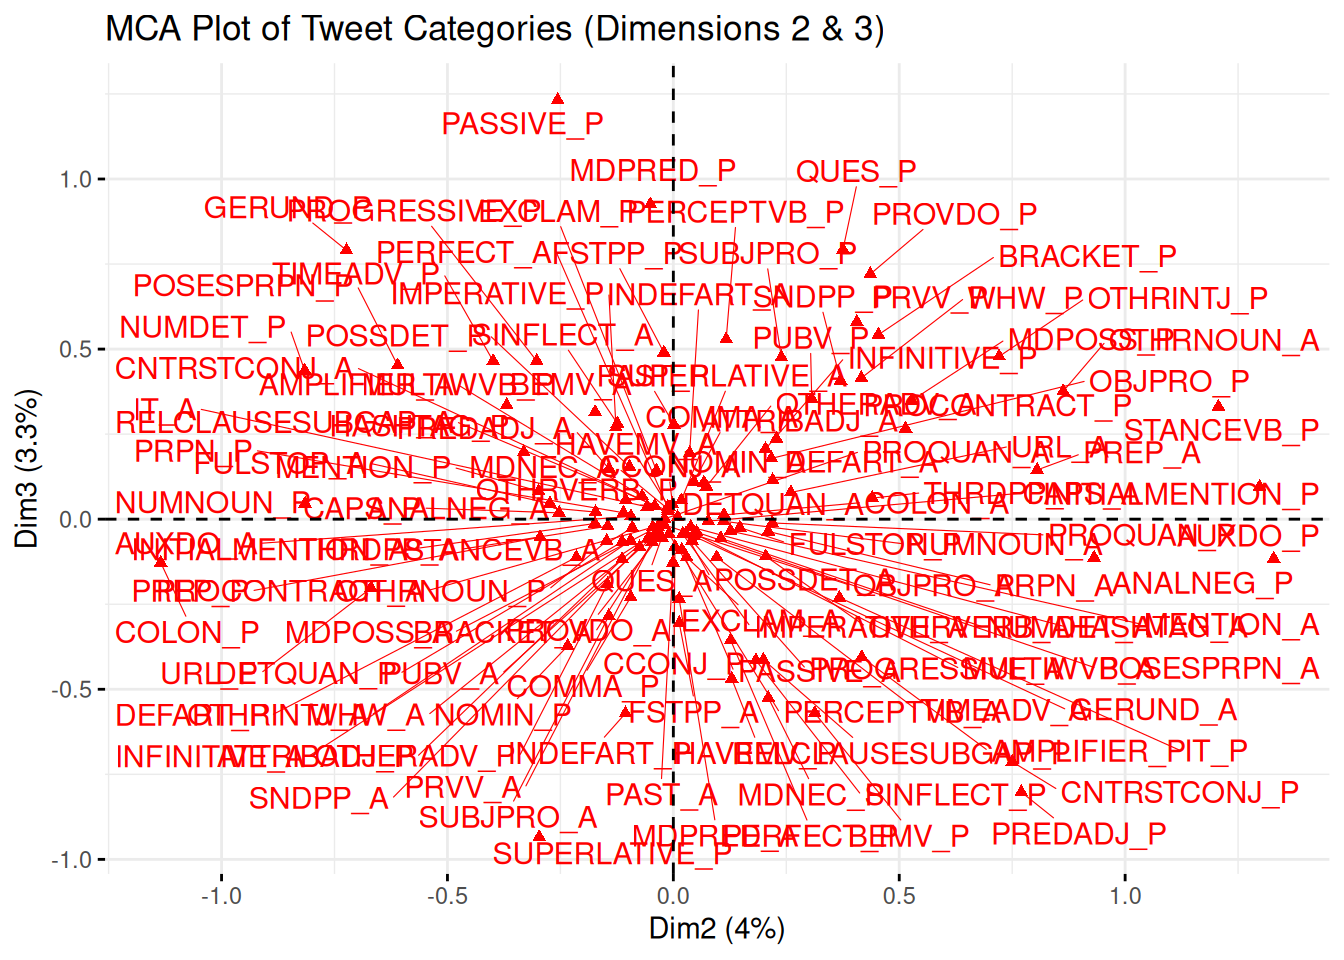
\includegraphics[keepaspectratio]{Introduction-to-Quantitative-Text-Analysis_files/figure-latex/trumptweets-fvizvar-1.pdf}}

This plot illustrates the relationships between the tweet categories based on Dimensions 2 and 3. Clarke \& Grieve (\citeproc{ref-Clarke2019a}{2019}) interpreted Dimension 2 as a `Conversational Style' and Dimension 3 as a `Campaigning Style'. Thus, categories at the extremes of Dimension 2 indicate conversational style, while those at the extremes of Dimension 3 are associated with campaigning style. Categories near the centre are less distinctive along these dimensions.

To see which categories contribute most to these dimensions or have the most extreme positions, we can examine their coordinates on the dimensions. The \texttt{get\_mca\_var()} function extracts detailed information about the variables (categories), including their coordinates, contributions to the dimensions, and correlations.

\begin{Shaded}
\begin{Highlighting}[]
\NormalTok{var\_info }\OtherTok{\textless{}{-}} \FunctionTok{get\_mca\_var}\NormalTok{(mca\_tweets)  }\CommentTok{\# Get detailed information about the categories (variables) from the MCA output.}
\NormalTok{coordinates }\OtherTok{\textless{}{-}} \FunctionTok{as.data.frame}\NormalTok{(var\_info}\SpecialCharTok{$}\NormalTok{coord)  }\CommentTok{\# Extract the coordinates of the categories on each dimension.}
\FunctionTok{head}\NormalTok{(coordinates)}
\end{Highlighting}
\end{Shaded}

\begin{verbatim}
##                   Dim 1       Dim 2       Dim 3       Dim 4       Dim 5
## AMPLIFIER_A -0.09788751 -0.06902274  0.06712121  0.09543741 -0.03446247
## AMPLIFIER_P  0.59146114  0.41705287 -0.40556335 -0.57665701  0.20823099
## ANALNEG_A   -0.15748770 -0.17213448  0.02091087 -0.09791397 -0.04902178
## ANALNEG_P    0.85204886  0.93129168 -0.11313318  0.52973968  0.26522042
## ATTRIBADJ_A -0.47929022  0.22824686  0.23663061  0.13986682  0.40121761
## ATTRIBADJ_P  0.23821011 -0.11344006 -0.11760683 -0.06951464 -0.19940755
\end{verbatim}

\begin{Shaded}
\begin{Highlighting}[]
\CommentTok{\# Optionally, order by a specific dimension to see the extremes. This can help}
\CommentTok{\# interpret the dimensions by identifying the categories most strongly}
\CommentTok{\# associated with each end.}

\NormalTok{coordinates\_ordered\_dim2 }\OtherTok{\textless{}{-}}\NormalTok{ coordinates }\SpecialCharTok{\%\textgreater{}\%}
    \FunctionTok{arrange}\NormalTok{(}\StringTok{\textasciigrave{}}\AttributeTok{Dim 2}\StringTok{\textasciigrave{}}\NormalTok{)}

\FunctionTok{head}\NormalTok{(coordinates\_ordered\_dim2)  }\CommentTok{\# Display categories with the most negative coordinates on Dim 2}
\end{Highlighting}
\end{Shaded}

\begin{verbatim}
##                  Dim 1      Dim 2       Dim 3       Dim 4      Dim 5
## COLON_P     -0.2592962 -1.1346550 -0.12765743  0.65087583  0.6419737
## NUMDET_P     0.3617208 -0.8159953  0.43697966 -0.03973954  0.1617759
## NUMNOUN_P    0.2506834 -0.8150235  0.04534697 -0.38332211  0.3973838
## GERUND_P     0.2383111 -0.7235272  0.79047745 -0.04533401 -0.3780261
## URL_P       -0.5334139 -0.6689921 -0.20223454  0.29823581  0.6217575
## POSESPRPN_P  0.1372452 -0.6100926  0.45200582  0.16700550  0.6420377
\end{verbatim}

\begin{Shaded}
\begin{Highlighting}[]
\FunctionTok{tail}\NormalTok{(coordinates\_ordered\_dim2)  }\CommentTok{\# Display categories with the most positive coordinates on Dim 2}
\end{Highlighting}
\end{Shaded}

\begin{verbatim}
##                       Dim 1     Dim 2       Dim 3       Dim 4       Dim 5
## PREP_A           -0.8230712 0.8052457  0.14477086 -0.03477667  0.03766616
## OTHRNOUN_A       -1.4568686 0.8629022  0.37599003 -0.41308773  0.09841326
## ANALNEG_P         0.8520489 0.9312917 -0.11313318  0.52973968  0.26522042
## STANCEVB_P        0.5514010 1.2065100  0.33043865  0.49040727  0.77609391
## INITIALMENTION_P -1.3740889 1.2977164  0.09504675 -0.65336128 -0.36025425
## AUXDO_P           0.7401893 1.3289167 -0.11606038  1.11590177  0.30943522
\end{verbatim}

\begin{Shaded}
\begin{Highlighting}[]
\NormalTok{coordinates\_ordered\_dim3 }\OtherTok{\textless{}{-}}\NormalTok{ coordinates }\SpecialCharTok{\%\textgreater{}\%}
    \FunctionTok{arrange}\NormalTok{(}\StringTok{\textasciigrave{}}\AttributeTok{Dim 3}\StringTok{\textasciigrave{}}\NormalTok{)}

\FunctionTok{head}\NormalTok{(coordinates\_ordered\_dim3)}
\end{Highlighting}
\end{Shaded}

\begin{verbatim}
##                   Dim 1      Dim 2      Dim 3       Dim 4       Dim 5
## SUPERLATIVE_P 0.3844324 -0.2969177 -0.9344720  0.37897964 -1.12086446
## PREDADJ_P     0.5907107  0.7702513 -0.8023569 -0.66156655  0.32914762
## CNTRSTCONJ_P  0.4785936  0.7500073 -0.7131886 -0.58944621  0.45511677
## INDEFART_P    0.4894847 -0.1060032 -0.5706842 -0.05053374  0.20323712
## BEMV_P        0.5529525  0.3132293 -0.5702540 -0.34951629  0.06513688
## MDNEC_P       0.5222506  0.2103261 -0.5253531  0.61481327  0.08689422
\end{verbatim}

\begin{Shaded}
\begin{Highlighting}[]
\FunctionTok{tail}\NormalTok{(coordinates\_ordered\_dim3)}
\end{Highlighting}
\end{Shaded}

\begin{verbatim}
##               Dim 1       Dim 2     Dim 3       Dim 4       Dim 5
## PRVV_P    0.6250762  0.40612075 0.5799258  0.79378561 -0.07698886
## PROVDO_P  1.0370597  0.43591147 0.7204183 -0.03205591 -0.66174907
## GERUND_P  0.2383111 -0.72352720 0.7904774 -0.04533401 -0.37802611
## QUES_P    0.3404573  0.37539603 0.7922378  1.57205964  0.26088244
## MDPRED_P  0.4722946 -0.05099973 0.9256090 -0.68949403 -0.08883854
## PASSIVE_P 0.6729391 -0.25613607 1.2319758 -1.15578164 -0.16784366
\end{verbatim}

Examining the categories with the highest absolute coordinates on Dimensions 2 and 3 provides insight into the characteristics of these stylistic dimensions. For instance, if categories such as `Use of colloquialisms' or `Personal anecdotes' have high positive coordinates on Dimension 2, this lends weight to interpreting this dimension as `Conversational Style'. Similarly, if categories such as `Policy mentions' or `Calls to action' have high positive coordinates on Dimension 3, this would support the interpretation of this dimension as `Campaigning Style'. MCA also enables individuals (or, in this case, tweets) to be plotted in the same space using the \texttt{fviz\_mca\_ind()} function, which can reveal clusters of tweets with similar stylistic features:

\begin{Shaded}
\begin{Highlighting}[]
\CommentTok{\# Plot the position of individual tweets on Dimensions 2 and 3.}
\FunctionTok{fviz\_mca\_ind}\NormalTok{(mca\_tweets,}
             \AttributeTok{geom =} \StringTok{"point"}\NormalTok{, }\CommentTok{\# Show points for each tweet}
             \AttributeTok{axes =} \FunctionTok{c}\NormalTok{(}\DecValTok{2}\NormalTok{, }\DecValTok{3}\NormalTok{), }\CommentTok{\# Plot Dimensions 2 and 3}
             \AttributeTok{col.ind =} \StringTok{"cos2"}\NormalTok{, }\AttributeTok{gradient.cols =} \FunctionTok{c}\NormalTok{(}\StringTok{"\#00AFBB"}\NormalTok{, }\StringTok{"\#E7B800"}\NormalTok{, }\StringTok{"\#FC4E07"}\NormalTok{), }\CommentTok{\# Color individuals by their quality of representation (cos2) on the dimensions, using a colour gradient}
             \AttributeTok{repel =} \ConstantTok{FALSE}\NormalTok{,}
             \AttributeTok{ggtheme =} \FunctionTok{theme\_minimal}\NormalTok{(),}
             \AttributeTok{title =} \StringTok{"MCA Plot of Individual Tweets (Dimensions 2 \& 3)"}\NormalTok{)}
\end{Highlighting}
\end{Shaded}

\pandocbounded{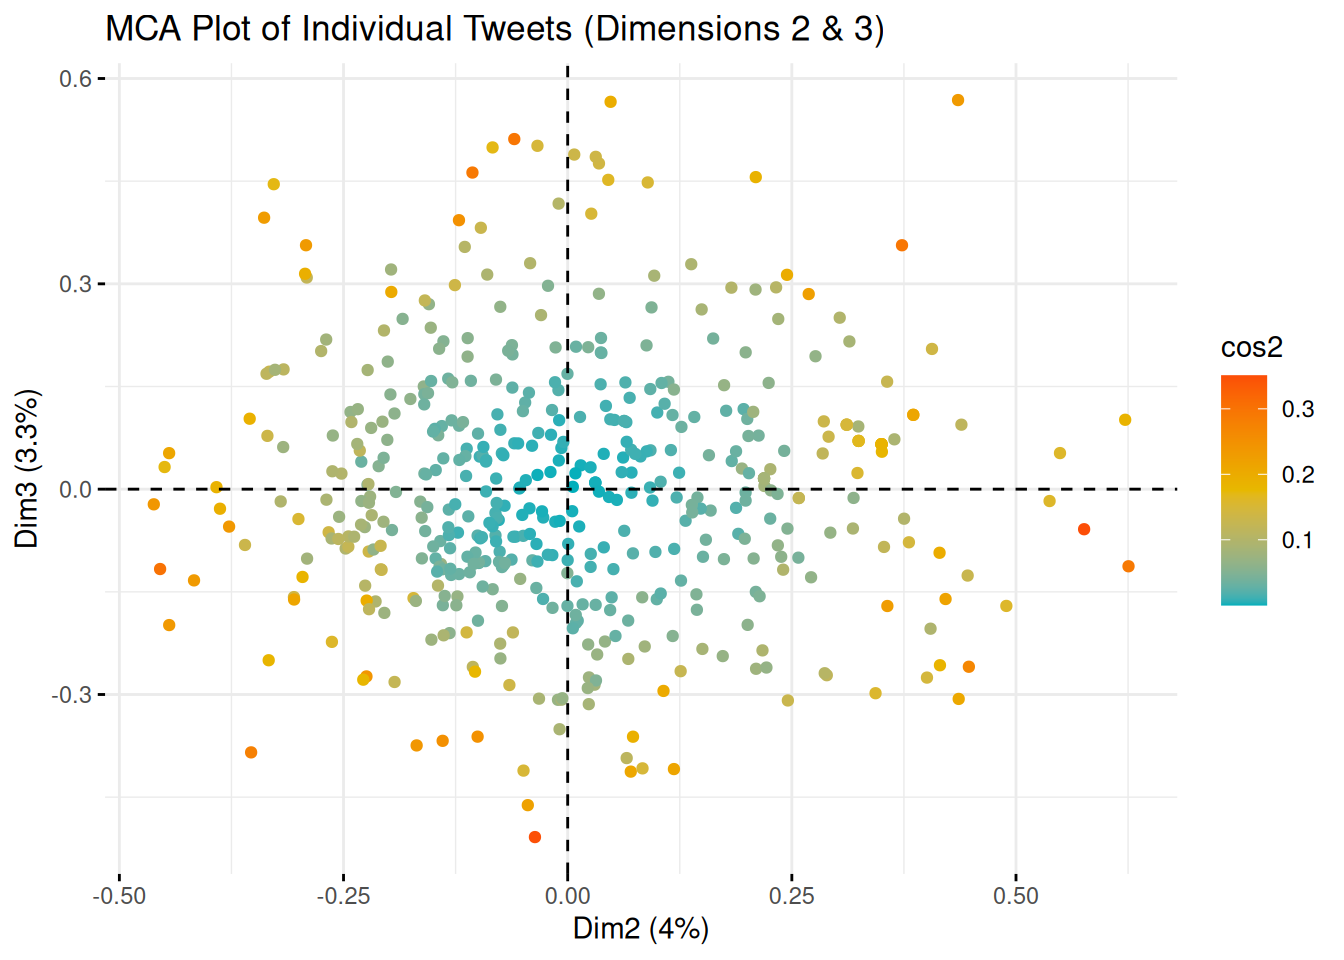
\includegraphics[keepaspectratio]{Introduction-to-Quantitative-Text-Analysis_files/figure-latex/trumptweets-fvizind-1.pdf}}

Interpreting MCA results is often an iterative and exploratory process that involves examining the position of categories and individuals and potentially using additional variables or external information to understand the meaning of the dimensions. The designers of \texttt{FactoMineR} have developed a Shiny app called \texttt{Factoshiny} that provides an interactive interface for exploring MCA results that can be very helpful in this process.

\begin{Shaded}
\begin{Highlighting}[]
\FunctionTok{library}\NormalTok{(Factoshiny)}

\CommentTok{\# Launch the interactive Shiny app for MCA results. This provides a graphical}
\CommentTok{\# user interface to explore the MCA output interactively}

\NormalTok{res.shiny }\OtherTok{\textless{}{-}} \FunctionTok{MCAshiny}\NormalTok{(mca\_tweets)  }\CommentTok{\# Use the MCA output object as input.}
\end{Highlighting}
\end{Shaded}

Ensure you quit the Shiny application by clicking the ``Quit the App'' button to return to your R session. For more information on Correspondence Analysis and the \texttt{FactoMineR} package, see the original article by Lê et al. (\citeproc{ref-Le2008a}{2008}) or the package website.

While \texttt{FactoMineR} is excellent for MCA with pre-coded categorical data, the \texttt{quanteda.textmodels} package also provides a function, \texttt{textmodel\_ca()}, designed explicitly for Simple Correspondence Analysis (SCA) on a document-feature matrix (dfm). This is particularly useful when you want to perform CA directly on raw term frequencies in your corpus without prior categorisation. Based on their co-occurrence patterns, SCA on a dfm positions both documents and terms in a low-dimensional space.

Let's apply \texttt{textmodel\_ca()} to the UK party manifestos dfm we created earlier in the Wordscores section. We will fit an SCA model and then explore the resulting document and feature placements. First, ensure you have loaded the \texttt{quanteda.textmodels} package. Then, we can apply the \texttt{textmodel\_ca()} function to our \texttt{data\_manifestos\_dfm}, for which we must specify the number of dimensions (\texttt{nd}) to compute:

\begin{Shaded}
\begin{Highlighting}[]
\CommentTok{\# Ensure quanteda.textmodels is loaded}
\FunctionTok{library}\NormalTok{(quanteda.textmodels)}

\CommentTok{\# We will compute the first 2 dimensions}
\NormalTok{ca\_model }\OtherTok{\textless{}{-}} \FunctionTok{textmodel\_ca}\NormalTok{(data\_manifestos\_dfm, }\AttributeTok{nd =} \DecValTok{2}\NormalTok{)}
\NormalTok{ca\_model}\SpecialCharTok{$}\NormalTok{sv}
\end{Highlighting}
\end{Shaded}

\begin{verbatim}
## [1] 0.5276873 0.4724757
\end{verbatim}

The output for \texttt{textmodel\_ca} shows the eigenvalues for the first two dimensions, indicating the amount of variance explained by each dimension. The \texttt{ca\_model} object also provides the coordinates of both features (terms) and documents on the computed dimensions. Features or documents with similar coordinates are located close together in the CA space, suggesting a strong association based on their co-occurrence patterns. We can access the coordinates of the documents and features directly from the model object for plotting. The document coordinates are stored in \texttt{ca\_model\$rowcoord}, and the feature coordinates are in \texttt{ca\_model\$colcoord}:

\begin{Shaded}
\begin{Highlighting}[]
\NormalTok{doc\_coords }\OtherTok{\textless{}{-}} \FunctionTok{as.data.frame}\NormalTok{(ca\_model}\SpecialCharTok{$}\NormalTok{rowcoord)}
\NormalTok{doc\_coords}\SpecialCharTok{$}\NormalTok{document }\OtherTok{\textless{}{-}} \FunctionTok{rownames}\NormalTok{(doc\_coords)}
\FunctionTok{head}\NormalTok{(doc\_coords)}
\end{Highlighting}
\end{Shaded}

\begin{verbatim}
##                           Dim1       Dim2            document
## UK_natl_2001_en_Con  0.1524448 -0.5672257 UK_natl_2001_en_Con
## UK_natl_2001_en_Lab  0.3302092 -0.5700563 UK_natl_2001_en_Lab
## UK_natl_2001_en_LD   0.1771004  0.2938892  UK_natl_2001_en_LD
## UK_natl_2001_en_PCy  0.1031924  2.8146966 UK_natl_2001_en_PCy
## UK_natl_2001_en_SNP -0.8278683  0.8287998 UK_natl_2001_en_SNP
## UK_natl_2005_en_Con  0.1432759 -1.0469080 UK_natl_2005_en_Con
\end{verbatim}

\begin{Shaded}
\begin{Highlighting}[]
\CommentTok{\# Extract feature coordinates}

\NormalTok{feature\_coords }\OtherTok{\textless{}{-}} \FunctionTok{as.data.frame}\NormalTok{(ca\_model}\SpecialCharTok{$}\NormalTok{colcoord)}
\NormalTok{feature\_coords}\SpecialCharTok{$}\NormalTok{feature }\OtherTok{\textless{}{-}} \FunctionTok{rownames}\NormalTok{(feature\_coords)}
\FunctionTok{head}\NormalTok{(feature\_coords)}
\end{Highlighting}
\end{Shaded}

\begin{verbatim}
##                    Dim1       Dim2      feature
## time          0.1959597 -0.3493652         time
## common        0.2421251 -0.6085238       common
## sense         0.3245334 -1.0271480        sense
## conservative  0.2831843 -1.3381374 conservative
## manifesto     0.2763475 -0.7723784    manifesto
## introduction -0.4311302  1.4987321 introduction
\end{verbatim}

Now that we have extracted the coordinates, we can visualise the documents and features in the CA space using \texttt{ggplot2}. Plotting both documents and features on the same plot enables us to inspect their relationships directly. Terms located near a document are likely to appear frequently compared to other documents, and documents located near each other tend to use similar vocabulary.

\begin{Shaded}
\begin{Highlighting}[]
\FunctionTok{library}\NormalTok{(ggplot2)}

\FunctionTok{ggplot}\NormalTok{() }\SpecialCharTok{+}
  \FunctionTok{geom\_point}\NormalTok{(}\AttributeTok{data =}\NormalTok{ doc\_coords, }\FunctionTok{aes}\NormalTok{(}\AttributeTok{x =}\NormalTok{ Dim1, }\AttributeTok{y =}\NormalTok{ Dim2, }\AttributeTok{color =}\NormalTok{ document), }\AttributeTok{size =} \DecValTok{3}\NormalTok{) }\SpecialCharTok{+} 
  \FunctionTok{geom\_text}\NormalTok{(}\AttributeTok{data =}\NormalTok{ doc\_coords, }\FunctionTok{aes}\NormalTok{(}\AttributeTok{x =}\NormalTok{ Dim1, }\AttributeTok{y =}\NormalTok{ Dim2, }\AttributeTok{label =}\NormalTok{ document), }\AttributeTok{vjust =} \FloatTok{1.5}\NormalTok{, }\AttributeTok{size =} \DecValTok{3}\NormalTok{) }\SpecialCharTok{+} \CommentTok{\# Add document labels}
  \FunctionTok{geom\_point}\NormalTok{(}\AttributeTok{data =}\NormalTok{ feature\_coords, }\FunctionTok{aes}\NormalTok{(}\AttributeTok{x =}\NormalTok{ Dim1, }\AttributeTok{y =}\NormalTok{ Dim2), }\AttributeTok{shape =} \DecValTok{3}\NormalTok{, }\AttributeTok{color =} \StringTok{"darkgrey"}\NormalTok{) }\SpecialCharTok{+} 
\FunctionTok{geom\_vline}\NormalTok{(}\AttributeTok{xintercept =} \DecValTok{0}\NormalTok{, }\AttributeTok{linetype =} \StringTok{"dashed"}\NormalTok{, }\AttributeTok{color =} \StringTok{"grey"}\NormalTok{) }\SpecialCharTok{+} \CommentTok{\# Add vertical line at x=0}
  \FunctionTok{geom\_hline}\NormalTok{(}\AttributeTok{yintercept =} \DecValTok{0}\NormalTok{, }\AttributeTok{linetype =} \StringTok{"dashed"}\NormalTok{, }\AttributeTok{color =} \StringTok{"grey"}\NormalTok{) }\SpecialCharTok{+} \CommentTok{\# Add horizontal line at y=0}
  \FunctionTok{ggtitle}\NormalTok{(}\StringTok{"Correspondence Analysis of UK Party Manifestos"}\NormalTok{) }\SpecialCharTok{+}
\FunctionTok{scale\_x\_continuous}\NormalTok{(}\AttributeTok{name =} \StringTok{"Dimension 1"}\NormalTok{) }\SpecialCharTok{+}
\FunctionTok{scale\_y\_continuous}\NormalTok{(}\AttributeTok{name =} \StringTok{"Dimension 2"}\NormalTok{) }\SpecialCharTok{+}
  \FunctionTok{theme\_minimal}\NormalTok{() }\SpecialCharTok{+}
  \FunctionTok{theme}\NormalTok{(}\AttributeTok{legend.position =} \StringTok{"none"}\NormalTok{)}
\end{Highlighting}
\end{Shaded}

\pandocbounded{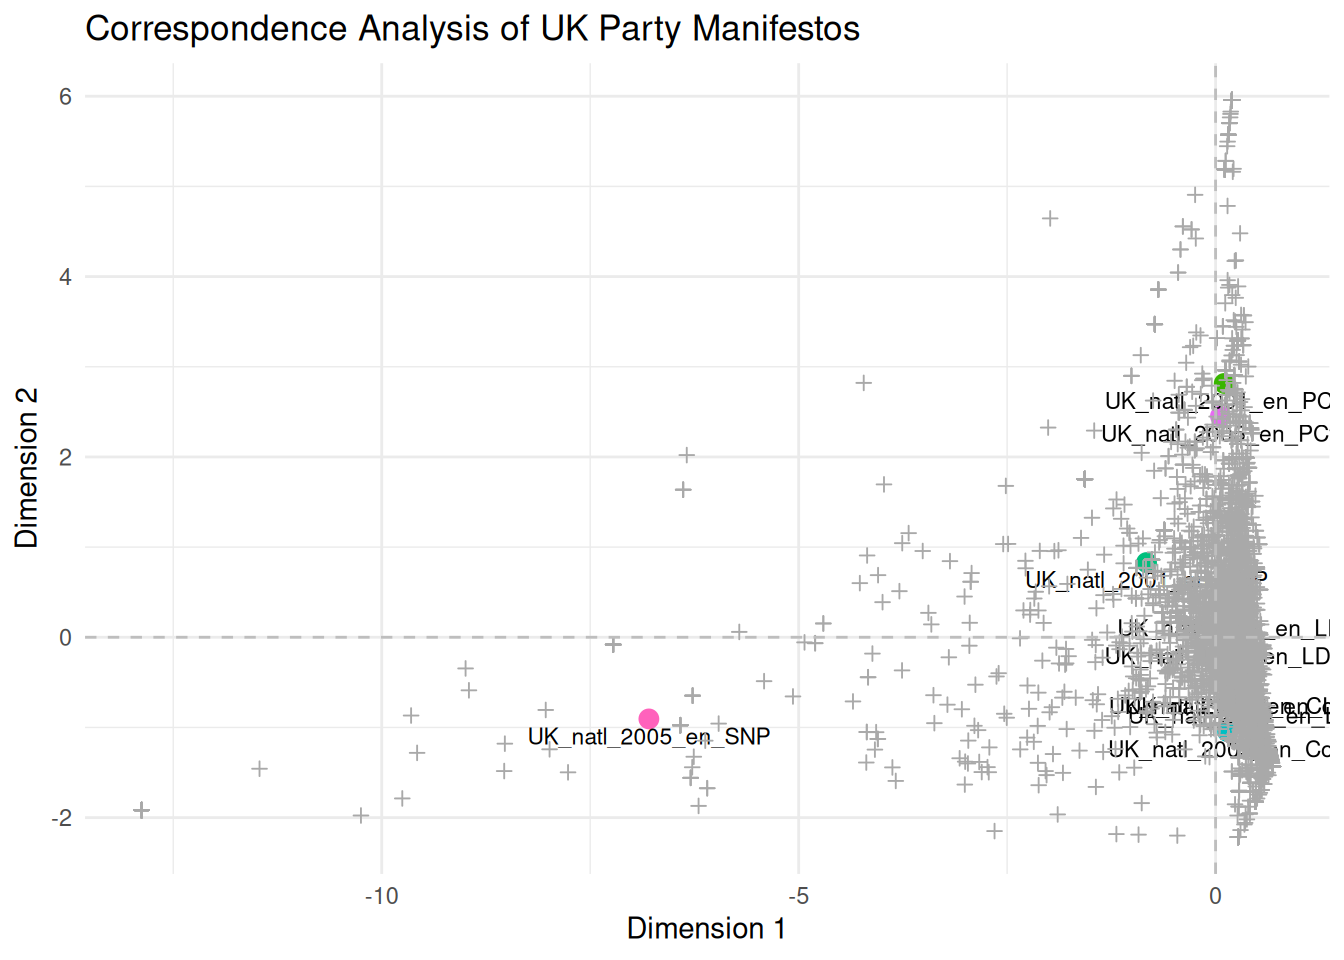
\includegraphics[keepaspectratio]{Introduction-to-Quantitative-Text-Analysis_files/figure-latex/ggplot-textmodelca-1.pdf}}

This plot illustrates the relative positions of UK party manifestos and terms extracted from the first two dimensions by SCA. Documents positioned closer together use similar vocabulary, and terms positioned closer to documents are more characteristic of them. The interpretation of the dimensions (e.g.~as a left-right scale or another thematic contrast) depends on examining which documents and terms fall at the extremes of each dimension. For instance, if manifestos from left-leaning parties and terms related to social welfare appear at one end of Dimension 1 and manifestos from right-leaning parties and terms related to the economy or security appear at the other, then Dimension 1 probably represents a left-right political spectrum.

\section{Exercises}\label{exercises-2}

\begin{enumerate}
\def\labelenumi{\arabic{enumi}.}
\item
  Apply the Wordscores method to the inaugural speeches corpus (data\_corpus\_inaugural). Select a set of reference speeches and assign them hypothetical scores based on a dimension of interest (e.g.~populism, as defined by external knowledge). Estimate the scores for the remaining speeches and visualise the results. Discuss the estimated positions and the uncertainty around them.
\item
  Apply the Wordfish method to the corpus of UK party manifestos used in the Wordscores example. Select two manifestos to define the direction of the scale. Interpret the resulting dimension based on the words that load highly on it and the manifestos' positions. Compare the Wordfish results with the Wordscores results.
\item
  Explore another dataset with categorical text annotations or create a categorised dataset from a text corpus (for example, by coding themes in a small set of documents). Perform Multiple Correspondence Analysis on this data. Interpret the main dimensions based on the categories that contribute most to them. Visualise the categories and/or individuals in the MCA space.
\item
  Apply Simple Correspondence Analysis to a document-feature matrix of your choice using the \texttt{textmodel\_ca()} function. Interpret the first two dimensions based on the words and documents located at the extremes. Visualise the results and discuss the relationships revealed by the plot.
\item
  Use the \texttt{textmodel\_affinity()} function to compute the affinity matrix for a corpus. Explore the matrix to identify documents with a high affinity to specific documents of interest. Apply a clustering method (e.g.~hierarchical clustering) to the affinity matrix and interpret the resulting clusters.
\item
  Research other scaling methods for text analysis, such as ideal point models or specialised techniques for specific text data types. How do they differ from Wordscores, Wordfish and Correspondence Analysis in terms of their assumptions and applications?
\end{enumerate}

\chapter{Supervised Methods}\label{supervised-methods}

Supervised learning methods use this pre-labelled data to recognise patterns. Think of it like a student learning from examples with answers provided by a teacher. Labelled data, also known as the training set, consists of a collection of texts, each of which has a known category or value assigned to it. Examples include movie reviews labelled as `positive' or `negative', news articles categorised by topic (e.g.~`sports', `politics', `finance'), and survey responses assigned a satisfaction score. A supervised learning algorithm examines the features of these labelled texts --- typically, which words appear and how often --- and tries to determine the relationship between the words and the labels. For instance, it may recognise that reviews containing words such as `amazing', `love' and `excellent' are often categorised as `positive'. Once the algorithm has learned these patterns from the training set, it can predict the labels of new, unlabelled texts --- usually called the test set.

Supervised methods are effective when manual labelling of a subset of data is feasible, but automatic classification of larger volumes of text is required. Supervised methods differ from dictionary methods, which rely on fixed lists of words, and unsupervised methods, such as topic modelling or clustering, which discover patterns without needing pre-assigned labels.

Several algorithms for supervised text classification are available within the R ecosystem, particularly those integrated with \texttt{quanteda}. We will cover two widely used, relatively simple yet effective algorithms: Support Vector Machines (SVM) and Naive Bayes (NB). SVM is a powerful discriminative classifier that identifies an optimal boundary, or hyperplane, to distinguish between different categories in a high-dimensional feature space. Naive Bayes is a probabilistic classifier based on Bayes' theorem, which simplifies the assumption that features are independent of each other.

We will also explore methods for visualising model performance and implementing cross-validation using the \texttt{caret} package, which provides a unified interface for many machine-learning algorithms and validation techniques.

\section{Support Vector Machines (SVM)}\label{support-vector-machines-svm}

SVMs are powerful supervised learning models that are frequently employed for classification tasks. In text classification, for example, they operate by mapping features of documents, such as word counts, from a document-feature matrix (DFM) into a high-dimensional space. In this space, SVMs identify the optimal hyperplane that most effectively separates documents into different categories.

Imagine you have a piece of paper with red and blue dots scattered on it, and you want to draw a straight line that best separates them. An SVM tries to do something similar but in many more dimensions. Each document can be considered a point in a very high-dimensional space. Each dimension corresponds to a unique word in your vocabulary, and the position of the document along that dimension depends on how frequently that word appears in the document or on other measures, such as TF-IDF. An SVM aims to find the optimal hyperplane that best separates documents into different categories, such as ``positive review'' versus ``negative review''. `Best' means the hyperplane with the largest possible margin --- the broadest possible gap --- between the closest documents of the different classes. Documents closest to this boundary, which defines the margin, are called `support vectors'. SVMs are known for their effectiveness, especially when dealing with many features, which is common in text data since each word can constitute a feature.

In this example, we will use the \texttt{caret} package to train an SVM model for binary polarity classification, use \texttt{quanteda} for text preprocessing and the binary polarity label (``neg'' or ``pos'') provided by a sample of the Large Movie Review Dataset (\texttt{data\_corpus\_LMRD}) as the target variable:

\begin{Shaded}
\begin{Highlighting}[]
\FunctionTok{set.seed}\NormalTok{(}\DecValTok{42}\NormalTok{)}

\FunctionTok{library}\NormalTok{(quanteda)}
\FunctionTok{library}\NormalTok{(quanteda.classifiers)}
\FunctionTok{library}\NormalTok{(caret)  }\CommentTok{\# For model training, evaluation, and cross{-}validation}
\FunctionTok{library}\NormalTok{(ggplot2)}
\FunctionTok{library}\NormalTok{(pROC)  }\CommentTok{\# For ROC analysis}

\NormalTok{corpus\_reviews }\OtherTok{\textless{}{-}} \FunctionTok{corpus\_sample}\NormalTok{(data\_corpus\_LMRD, }\DecValTok{2000}\NormalTok{)  }\CommentTok{\# Sample 2000 reviews}
\end{Highlighting}
\end{Shaded}

We need to split our data into separate training and test sets for supervised learning: we will use the training set to build the model and the test set to evaluate its performance on unseen data later on. We will use the \texttt{polarity} variable as our target, ensuring it is a factor as this is the required format for classification tasks in \texttt{caret}. Note that we will filter for documents with non-missing polarity labels before splitting. \texttt{caret} requires factor levels to be valid R variable names (like ``neg'' and ``pos''):

\begin{Shaded}
\begin{Highlighting}[]
\NormalTok{polarity\_labels }\OtherTok{\textless{}{-}} \FunctionTok{factor}\NormalTok{(corpus\_reviews}\SpecialCharTok{$}\NormalTok{polarity)}

\CommentTok{\# Identify documents with valid polarity labels}

\NormalTok{valid\_docs\_index }\OtherTok{\textless{}{-}} \FunctionTok{which}\NormalTok{(}\SpecialCharTok{!}\FunctionTok{is.na}\NormalTok{(polarity\_labels))}
\NormalTok{corpus\_reviews\_valid }\OtherTok{\textless{}{-}}\NormalTok{ corpus\_reviews[valid\_docs\_index]}
\NormalTok{polarity\_valid }\OtherTok{\textless{}{-}}\NormalTok{ polarity\_labels[valid\_docs\_index]}
\NormalTok{polarity\_valid }\OtherTok{\textless{}{-}} \FunctionTok{factor}\NormalTok{(polarity\_valid, }\AttributeTok{levels =} \FunctionTok{c}\NormalTok{(}\StringTok{"neg"}\NormalTok{, }\StringTok{"pos"}\NormalTok{))}

\CommentTok{\# Check the distribution of polarity\_valid BEFORE splitting}
\FunctionTok{print}\NormalTok{(}\FunctionTok{table}\NormalTok{(polarity\_valid))}
\end{Highlighting}
\end{Shaded}

\begin{verbatim}
## polarity_valid
##  neg  pos 
## 1023  977
\end{verbatim}

\begin{Shaded}
\begin{Highlighting}[]
\CommentTok{\# Create stratified split indices to ensure both classes are included in}
\CommentTok{\# train/test sets}
\NormalTok{neg\_indices }\OtherTok{\textless{}{-}} \FunctionTok{which}\NormalTok{(polarity\_valid }\SpecialCharTok{==} \StringTok{"neg"}\NormalTok{)}
\NormalTok{pos\_indices }\OtherTok{\textless{}{-}} \FunctionTok{which}\NormalTok{(polarity\_valid }\SpecialCharTok{==} \StringTok{"pos"}\NormalTok{)}

\CommentTok{\# Determine the number of instances for train/test per class (70/30 split)}
\FunctionTok{set.seed}\NormalTok{(}\DecValTok{42}\NormalTok{)}
\NormalTok{train\_size\_neg }\OtherTok{\textless{}{-}} \FunctionTok{floor}\NormalTok{(}\FloatTok{0.7} \SpecialCharTok{*} \FunctionTok{length}\NormalTok{(neg\_indices))}
\NormalTok{train\_size\_pos }\OtherTok{\textless{}{-}} \FunctionTok{floor}\NormalTok{(}\FloatTok{0.7} \SpecialCharTok{*} \FunctionTok{length}\NormalTok{(pos\_indices))}

\CommentTok{\# Sample indices for training set from each class}
\NormalTok{train\_indices\_neg }\OtherTok{\textless{}{-}} \FunctionTok{sample}\NormalTok{(neg\_indices, }\AttributeTok{size =}\NormalTok{ train\_size\_neg, }\AttributeTok{replace =} \ConstantTok{FALSE}\NormalTok{)}
\NormalTok{train\_indices\_pos }\OtherTok{\textless{}{-}} \FunctionTok{sample}\NormalTok{(pos\_indices, }\AttributeTok{size =}\NormalTok{ train\_size\_pos, }\AttributeTok{replace =} \ConstantTok{FALSE}\NormalTok{)}

\CommentTok{\# Combine training indices}
\NormalTok{train\_index }\OtherTok{\textless{}{-}} \FunctionTok{c}\NormalTok{(train\_indices\_neg, train\_indices\_pos)}

\CommentTok{\# The remaining indices are for the test set}
\NormalTok{all\_valid\_indices }\OtherTok{\textless{}{-}} \FunctionTok{seq\_along}\NormalTok{(polarity\_valid)}
\NormalTok{test\_index }\OtherTok{\textless{}{-}}\NormalTok{ all\_valid\_indices[}\SpecialCharTok{!}\NormalTok{all\_valid\_indices }\SpecialCharTok{\%in\%}\NormalTok{ train\_index]}

\CommentTok{\# Split the corpus subset and polarity labels into training and testing sets}
\CommentTok{\# using the determined indices}
\NormalTok{corpus\_reviews\_train }\OtherTok{\textless{}{-}}\NormalTok{ corpus\_reviews\_valid[train\_index]}
\NormalTok{corpus\_reviews\_test }\OtherTok{\textless{}{-}}\NormalTok{ corpus\_reviews\_valid[test\_index]}

\NormalTok{polarity\_train }\OtherTok{\textless{}{-}}\NormalTok{ polarity\_valid[train\_index]}
\NormalTok{polarity\_test }\OtherTok{\textless{}{-}}\NormalTok{ polarity\_valid[test\_index]}

\CommentTok{\# Check the distribution of the split}
\FunctionTok{print}\NormalTok{(}\StringTok{"Training set class distribution:"}\NormalTok{)}
\end{Highlighting}
\end{Shaded}

\begin{verbatim}
## [1] "Training set class distribution:"
\end{verbatim}

\begin{Shaded}
\begin{Highlighting}[]
\FunctionTok{print}\NormalTok{(}\FunctionTok{table}\NormalTok{(polarity\_train))}
\end{Highlighting}
\end{Shaded}

\begin{verbatim}
## polarity_train
## neg pos 
## 716 683
\end{verbatim}

\begin{Shaded}
\begin{Highlighting}[]
\FunctionTok{print}\NormalTok{(}\StringTok{"Testing set class distribution:"}\NormalTok{)}
\end{Highlighting}
\end{Shaded}

\begin{verbatim}
## [1] "Testing set class distribution:"
\end{verbatim}

\begin{Shaded}
\begin{Highlighting}[]
\FunctionTok{print}\NormalTok{(}\FunctionTok{table}\NormalTok{(polarity\_test))}
\end{Highlighting}
\end{Shaded}

\begin{verbatim}
## polarity_test
## neg pos 
## 307 294
\end{verbatim}

Next, we preprocess the training and test corpus subsets to generate the DFMs. Here, it is crucial that the test DFM has the same features and order as the training DFM. The \texttt{dfm\_match()} function ensures this. We will then apply common text cleaning steps during tokenisation and convert the DFMs to matrices to ensure compatibility with \texttt{caret}.

\begin{Shaded}
\begin{Highlighting}[]
\CommentTok{\# Tokenise and preprocess the training corpus}

\NormalTok{tokens\_train }\OtherTok{\textless{}{-}} \FunctionTok{tokens}\NormalTok{(corpus\_reviews\_train, }\AttributeTok{what =} \StringTok{"word"}\NormalTok{, }\AttributeTok{remove\_punct =} \ConstantTok{TRUE}\NormalTok{,}
    \AttributeTok{remove\_symbols =} \ConstantTok{TRUE}\NormalTok{, }\AttributeTok{remove\_numbers =} \ConstantTok{TRUE}\NormalTok{, }\AttributeTok{remove\_url =} \ConstantTok{TRUE}\NormalTok{, }\AttributeTok{remove\_separators =} \ConstantTok{TRUE}\NormalTok{) }\SpecialCharTok{\%\textgreater{}\%}
    \FunctionTok{tokens\_tolower}\NormalTok{() }\SpecialCharTok{\%\textgreater{}\%}
    \FunctionTok{tokens\_select}\NormalTok{(}\FunctionTok{stopwords}\NormalTok{(}\StringTok{"english"}\NormalTok{), }\AttributeTok{selection =} \StringTok{"remove"}\NormalTok{)}

\CommentTok{\# Tokenise and preprocess the test corpus}

\NormalTok{tokens\_test }\OtherTok{\textless{}{-}} \FunctionTok{tokens}\NormalTok{(corpus\_reviews\_test, }\AttributeTok{what =} \StringTok{"word"}\NormalTok{, }\AttributeTok{remove\_punct =} \ConstantTok{TRUE}\NormalTok{, }\AttributeTok{remove\_symbols =} \ConstantTok{TRUE}\NormalTok{,}
    \AttributeTok{remove\_numbers =} \ConstantTok{TRUE}\NormalTok{, }\AttributeTok{remove\_url =} \ConstantTok{TRUE}\NormalTok{, }\AttributeTok{remove\_separators =} \ConstantTok{TRUE}\NormalTok{) }\SpecialCharTok{\%\textgreater{}\%}
    \FunctionTok{tokens\_tolower}\NormalTok{() }\SpecialCharTok{\%\textgreater{}\%}
    \FunctionTok{tokens\_select}\NormalTok{(}\FunctionTok{stopwords}\NormalTok{(}\StringTok{"english"}\NormalTok{), }\AttributeTok{selection =} \StringTok{"remove"}\NormalTok{)}

\CommentTok{\# Create DFMs from the processed tokens}

\NormalTok{dfm\_train }\OtherTok{\textless{}{-}} \FunctionTok{dfm}\NormalTok{(tokens\_train)}
\NormalTok{dfm\_test }\OtherTok{\textless{}{-}} \FunctionTok{dfm}\NormalTok{(tokens\_test)}

\CommentTok{\# Ensure the test DFM has the same features as the training DFM}

\NormalTok{dfm\_test\_matched }\OtherTok{\textless{}{-}} \FunctionTok{dfm\_match}\NormalTok{(dfm\_test, }\AttributeTok{features =} \FunctionTok{featnames}\NormalTok{(dfm\_train))}

\CommentTok{\# Convert DFMs to matrices for caret}

\NormalTok{matrix\_train }\OtherTok{\textless{}{-}} \FunctionTok{as.matrix}\NormalTok{(dfm\_train)}
\NormalTok{matrix\_test }\OtherTok{\textless{}{-}} \FunctionTok{as.matrix}\NormalTok{(dfm\_test\_matched)}

\CommentTok{\# Remove any zero{-}variance columns from the training matrix, as caret::train}
\CommentTok{\# can have issues Ensure the test matrix also has these columns removed}

\NormalTok{nzv\_train }\OtherTok{\textless{}{-}} \FunctionTok{nearZeroVar}\NormalTok{(matrix\_train)}
\ControlFlowTok{if}\NormalTok{ (}\FunctionTok{length}\NormalTok{(nzv\_train) }\SpecialCharTok{\textgreater{}} \DecValTok{0}\NormalTok{) \{}
\NormalTok{    matrix\_train }\OtherTok{\textless{}{-}}\NormalTok{ matrix\_train[, }\SpecialCharTok{{-}}\NormalTok{nzv\_train]}
\NormalTok{    matrix\_test }\OtherTok{\textless{}{-}}\NormalTok{ matrix\_test[, }\SpecialCharTok{{-}}\NormalTok{nzv\_train]}
\NormalTok{\}}
\end{Highlighting}
\end{Shaded}

Now we train the SVM model using \texttt{caret::train()}. \texttt{caret::train()} provides a consistent interface for training various models. We specify \texttt{method\ =\ "svmLinear"} for a linear kernel SVM, which is often a good starting point for text data.

Rather than using a single train/test split, we can use k-fold cross-validation to obtain a more reliable estimate of the model's performance. The \texttt{caret::train()} function makes this easy using the \texttt{trControl} argument. To demonstrate this, we will define a 10-fold cross-validation set-up. For binary classification, the \texttt{twoClassSummary} function calculates metrics such as accuracy, kappa, sensitivity, specificity, and ROC AUC.

What is k-fold cross-validation? Put simply, it involves splitting the training data into equal-sized parts, known as `folds'. For instance, if k equals 10, the training data would be divided into ten folds, and the model would be trained ten times. During each iteration, one fold is held out as a validation set and the model is trained using the remaining 9 folds. The trained model is then tested on the held-out validation set, and the performance metrics are recorded. After ten iterations, the performance metrics from each fold are averaged to provide a more reliable estimate of how the model will perform on new data.

The `caret' package makes cross-validation easy. We use the \texttt{trainControl()} function to specify the cross-validation settings and the \texttt{train()} function to train the model. We select a linear SVM using the argument \texttt{method\ =\ "svmLinear"}. Linear SVMs are often very effective and computationally less intensive than non-linear ones for text. Setting \texttt{metric\ =\ "ROC"} instructs caret to optimise the model based on the area under the ROC curve (AUC), a typical and effective metric for binary classification. Setting \texttt{classProbs\ =\ TRUE} means that we require the model to output class probabilities for ROC analysis and calibration plots, such as the probability that a review is `positive'. \texttt{summaryFunction\ =\ twoClassSummary} is used for binary classification problems and calculates useful metrics such as sensitivity, specificity, and ROC AUC during cross-validation.

\begin{Shaded}
\begin{Highlighting}[]
\NormalTok{train\_control\_cv\_clf }\OtherTok{\textless{}{-}} \FunctionTok{trainControl}\NormalTok{(}
  \AttributeTok{method =} \StringTok{"cv"}\NormalTok{,          }\CommentTok{\# Use cross{-}validation}
  \AttributeTok{number =} \DecValTok{10}\NormalTok{,            }\CommentTok{\# Number of folds}
  \AttributeTok{savePredictions =} \StringTok{"final"}\NormalTok{, }\CommentTok{\# Save predictions for the final model}
  \AttributeTok{classProbs =} \ConstantTok{TRUE}\NormalTok{,    }\CommentTok{\# Compute class probabilities (needed for ROC/Calibration)}
  \AttributeTok{summaryFunction =}\NormalTok{ twoClassSummary }\CommentTok{\# Use metrics suitable for binary classification}
\NormalTok{)}

\CommentTok{\# Train the SVM model using caret::train with cross{-}validation}
\CommentTok{\# We use svmLinear as the method}
\CommentTok{\# metric = "ROC" tells caret to optimise based on AUC}
\CommentTok{\# Ensure the factor levels for y (polarity\_train) are valid R names ("neg", "pos")}

\NormalTok{svm\_model\_caret\_cv }\OtherTok{\textless{}{-}} \FunctionTok{train}\NormalTok{(}
  \AttributeTok{x =}\NormalTok{ matrix\_train,      }\CommentTok{\# Training feature matrix}
  \AttributeTok{y =}\NormalTok{ polarity\_train,     }\CommentTok{\# Training response vector (factor: "neg", "pos")}
  \AttributeTok{method =} \StringTok{"svmLinear"}\NormalTok{, }\CommentTok{\# Use linear kernel SVM}
  \AttributeTok{trControl =}\NormalTok{ train\_control\_cv\_clf, }\CommentTok{\# Apply cross{-}validation control for classification}
  \AttributeTok{metric =} \StringTok{"ROC"}         \CommentTok{\# Optimize based on ROC AUC}
\NormalTok{)}

\FunctionTok{print}\NormalTok{(svm\_model\_caret\_cv)}
\end{Highlighting}
\end{Shaded}

\begin{verbatim}
## Support Vector Machines with Linear Kernel 
## 
## 1399 samples
##  245 predictor
##    2 classes: 'neg', 'pos' 
## 
## No pre-processing
## Resampling: Cross-Validated (10 fold) 
## Summary of sample sizes: 1260, 1258, 1258, 1260, 1260, 1259, ... 
## Resampling results:
## 
##   ROC        Sens       Spec     
##   0.7917106  0.7347418  0.7174979
## 
## Tuning parameter 'C' was held constant at a value of 1
\end{verbatim}

The output from \texttt{print(svm\_model\_caret\_cv)} now includes the average classification performance metrics, like Accuracy, Kappa, and ROC AUC, across the 10 folds. This provides a more accurate prediction of how the model will perform on unseen data than a single split would. We then use the trained \texttt{svm\_model\_caret\_cv} to predict the polarity labels and probabilities for the documents in the test set.

\begin{Shaded}
\begin{Highlighting}[]
\CommentTok{\# Predict the labels for the test set}
\NormalTok{svm\_predict\_labels\_caret\_cv }\OtherTok{\textless{}{-}} \FunctionTok{predict}\NormalTok{(svm\_model\_caret\_cv, }\AttributeTok{newdata =}\NormalTok{ matrix\_test)}

\CommentTok{\# Predict probabilities for the test set (needed for ROC and Calibration)}
\NormalTok{svm\_predict\_probs\_caret\_cv }\OtherTok{\textless{}{-}} \FunctionTok{predict}\NormalTok{(svm\_model\_caret\_cv, }\AttributeTok{newdata =}\NormalTok{ matrix\_test,}
    \AttributeTok{type =} \StringTok{"prob"}\NormalTok{)}

\CommentTok{\# Display the head of the predicted labels and probabilities}
\FunctionTok{head}\NormalTok{(svm\_predict\_labels\_caret\_cv)}
\end{Highlighting}
\end{Shaded}

\begin{verbatim}
## [1] pos neg pos neg neg pos
## Levels: neg pos
\end{verbatim}

\begin{Shaded}
\begin{Highlighting}[]
\FunctionTok{head}\NormalTok{(svm\_predict\_probs\_caret\_cv)}
\end{Highlighting}
\end{Shaded}

\begin{verbatim}
##         neg       pos
## 1 0.4393709 0.5606291
## 2 0.5076856 0.4923144
## 3 0.4927485 0.5072515
## 4 0.5997361 0.4002639
## 5 0.6494433 0.3505567
## 6 0.4764429 0.5235571
\end{verbatim}

Furthermore, we can examine the classification performance using \texttt{caret::confusionMatrix()} to compare the predicted and actual labels for the test set. This Confusion Matrix is a fundamental tool for evaluating classification models. It is a table that summarises performance by showing:

\begin{itemize}
\tightlist
\item
  \textbf{True Positives (TP)}: instances that were correctly predicted as positive
\item
  \textbf{True Negatives (TN)}: instances that were correctly predicted as negative
\item
  \textbf{False Positives (FP)}: instances that were incorrectly predicted as positive
\item
  \textbf{False Negatives (FN)}: instances that were incorrectly predicted as negative
\end{itemize}

From these counts, various metrics are derived:

\begin{itemize}
\tightlist
\item
  \textbf{Accuracy: (TP + TN) / Total}, representing overall correctness. However, it can be misleading if the classes are imbalanced;
\item
  \textbf{Sensitivity: TP/(TP+FN)}, indicating how well the model identifies actual positives;
\item
  \textbf{Specificity: TN/(TN+FP)}, showing how well the model identifies actual negatives;
\item
  \textbf{Precision: TP/(TP+FP)}, showing the proportion of predicted positives that were actually positive;
\item
  \textbf{F1-score: 2 * (Precision * Recall) / (Precision + Recall)}, the harmonic mean of precision and recall, is useful when both are important.
\end{itemize}

\begin{Shaded}
\begin{Highlighting}[]
\CommentTok{\# Ensure the reference (polarity\_test) has the same valid levels as the predicted data}

\NormalTok{confusion\_matrix\_caret\_cv }\OtherTok{\textless{}{-}} \FunctionTok{confusionMatrix}\NormalTok{(}
  \AttributeTok{data =}\NormalTok{ svm\_predict\_labels\_caret\_cv, }\CommentTok{\# Predicted labels (factor)}
  \AttributeTok{reference =}\NormalTok{ polarity\_test            }\CommentTok{\# Actual labels (reference factor)}
\NormalTok{)}

\CommentTok{\# Print the confusion matrix and performance statistics}
\FunctionTok{print}\NormalTok{(confusion\_matrix\_caret\_cv)}
\end{Highlighting}
\end{Shaded}

\begin{verbatim}
## Confusion Matrix and Statistics
## 
##           Reference
## Prediction neg pos
##        neg 219  70
##        pos  88 224
##                                        
##                Accuracy : 0.7371       
##                  95% CI : (0.7, 0.7719)
##     No Information Rate : 0.5108       
##     P-Value [Acc > NIR] : <2e-16       
##                                        
##                   Kappa : 0.4746       
##                                        
##  Mcnemar's Test P-Value : 0.1762       
##                                        
##             Sensitivity : 0.7134       
##             Specificity : 0.7619       
##          Pos Pred Value : 0.7578       
##          Neg Pred Value : 0.7179       
##              Prevalence : 0.5108       
##          Detection Rate : 0.3644       
##    Detection Prevalence : 0.4809       
##       Balanced Accuracy : 0.7376       
##                                        
##        'Positive' Class : neg          
## 
\end{verbatim}

The confusion matrix for the test set --- not used during the cross-validation training process --- provides a final evaluation of how well the model performs on data that has never been seen before. It shows the number of true positives, false positives and false negatives, from which various metrics can be derived. Finally, we can visualize all this:

\begin{Shaded}
\begin{Highlighting}[]
\NormalTok{cm\_table }\OtherTok{\textless{}{-}} \FunctionTok{as.data.frame}\NormalTok{(confusion\_matrix\_caret\_cv}\SpecialCharTok{$}\NormalTok{table)}

\FunctionTok{ggplot}\NormalTok{(}\AttributeTok{data =}\NormalTok{ cm\_table,}
       \FunctionTok{aes}\NormalTok{(}\AttributeTok{x =}\NormalTok{ Reference, }\AttributeTok{y =}\NormalTok{ Prediction, }\AttributeTok{fill =}\NormalTok{ Freq)) }\SpecialCharTok{+}
  \FunctionTok{geom\_tile}\NormalTok{() }\SpecialCharTok{+}
  \FunctionTok{geom\_text}\NormalTok{(}\FunctionTok{aes}\NormalTok{(}\AttributeTok{label =}\NormalTok{ Freq), }\AttributeTok{vjust =} \DecValTok{1}\NormalTok{, }\AttributeTok{color =} \StringTok{"black"}\NormalTok{) }\SpecialCharTok{+} \CommentTok{\# Add text labels for counts}
  \FunctionTok{scale\_fill\_gradient}\NormalTok{(}\AttributeTok{low =} \StringTok{"white"}\NormalTok{, }\AttributeTok{high =} \StringTok{"steelblue"}\NormalTok{) }\SpecialCharTok{+} \CommentTok{\# Colour scale}
  \FunctionTok{scale\_x\_discrete}\NormalTok{(}\AttributeTok{name =} \StringTok{"Actual Polarity"}\NormalTok{) }\SpecialCharTok{+}
  \FunctionTok{scale\_x\_discrete}\NormalTok{(}\AttributeTok{name =} \StringTok{"Predicted Polarity"}\NormalTok{) }\SpecialCharTok{+}
  \FunctionTok{ggtitle}\NormalTok{(}\StringTok{"Confusion Matrix (SVM Test Set)"}\NormalTok{) }\SpecialCharTok{+}
  \FunctionTok{theme\_minimal}\NormalTok{() }\SpecialCharTok{+} \CommentTok{\# Use a minimal theme}
  \FunctionTok{theme}\NormalTok{(}\AttributeTok{axis.text.x =} \FunctionTok{element\_text}\NormalTok{(}\AttributeTok{angle =} \DecValTok{45}\NormalTok{, }\AttributeTok{hjust =} \DecValTok{1}\NormalTok{)) }\CommentTok{\# Rotate x{-}axis labels if needed}
\end{Highlighting}
\end{Shaded}

\begin{verbatim}
## Scale for x is already present.
## Adding another scale for x, which will replace the existing scale.
\end{verbatim}

\pandocbounded{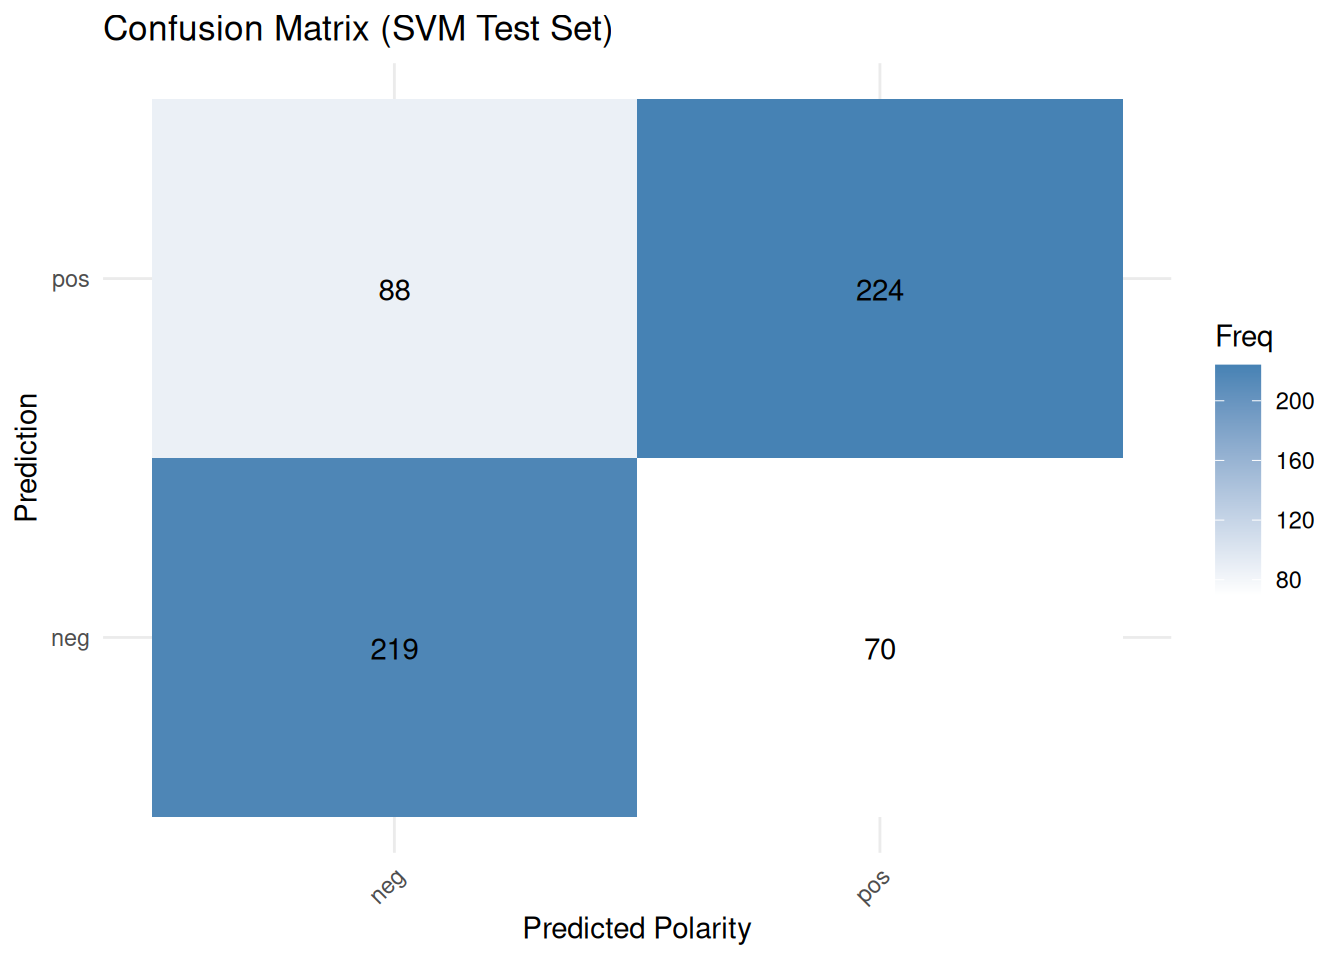
\includegraphics[keepaspectratio]{Introduction-to-Quantitative-Text-Analysis_files/figure-latex/svm-polarity-confusion-graph-1.pdf}}

In classification using linear SVMs, variable importance is usually related to the size of the model coefficients, showing which features contribute most to class separation. The \texttt{caret::varImp()} function can extract this information:

\begin{Shaded}
\begin{Highlighting}[]
\NormalTok{var\_importance\_svm }\OtherTok{\textless{}{-}} \FunctionTok{varImp}\NormalTok{(svm\_model\_caret\_cv, }\AttributeTok{scale =} \ConstantTok{FALSE}\NormalTok{)}

\CommentTok{\# Print the variable importance}
\FunctionTok{print}\NormalTok{(var\_importance\_svm)}
\end{Highlighting}
\end{Shaded}

\begin{verbatim}
## ROC curve variable importance
## 
##   only 20 most important variables shown (out of 245)
## 
##           Importance
## bad           0.6239
## great         0.5993
## worst         0.5731
## even          0.5653
## movie         0.5547
## best          0.5508
## love          0.5490
## just          0.5484
## acting        0.5479
## plot          0.5464
## many          0.5449
## waste         0.5424
## also          0.5417
## nothing       0.5413
## minutes       0.5404
## better        0.5399
## boring        0.5399
## like          0.5398
## worse         0.5395
## excellent     0.5391
\end{verbatim}

\begin{Shaded}
\begin{Highlighting}[]
\CommentTok{\# Plot the top 20 most important variables}
\FunctionTok{plot}\NormalTok{(var\_importance\_svm, }\AttributeTok{top =} \DecValTok{20}\NormalTok{, }\AttributeTok{main =} \StringTok{"Variable Importance (SVM {-} Top 20 words)"}\NormalTok{)}
\end{Highlighting}
\end{Shaded}

\pandocbounded{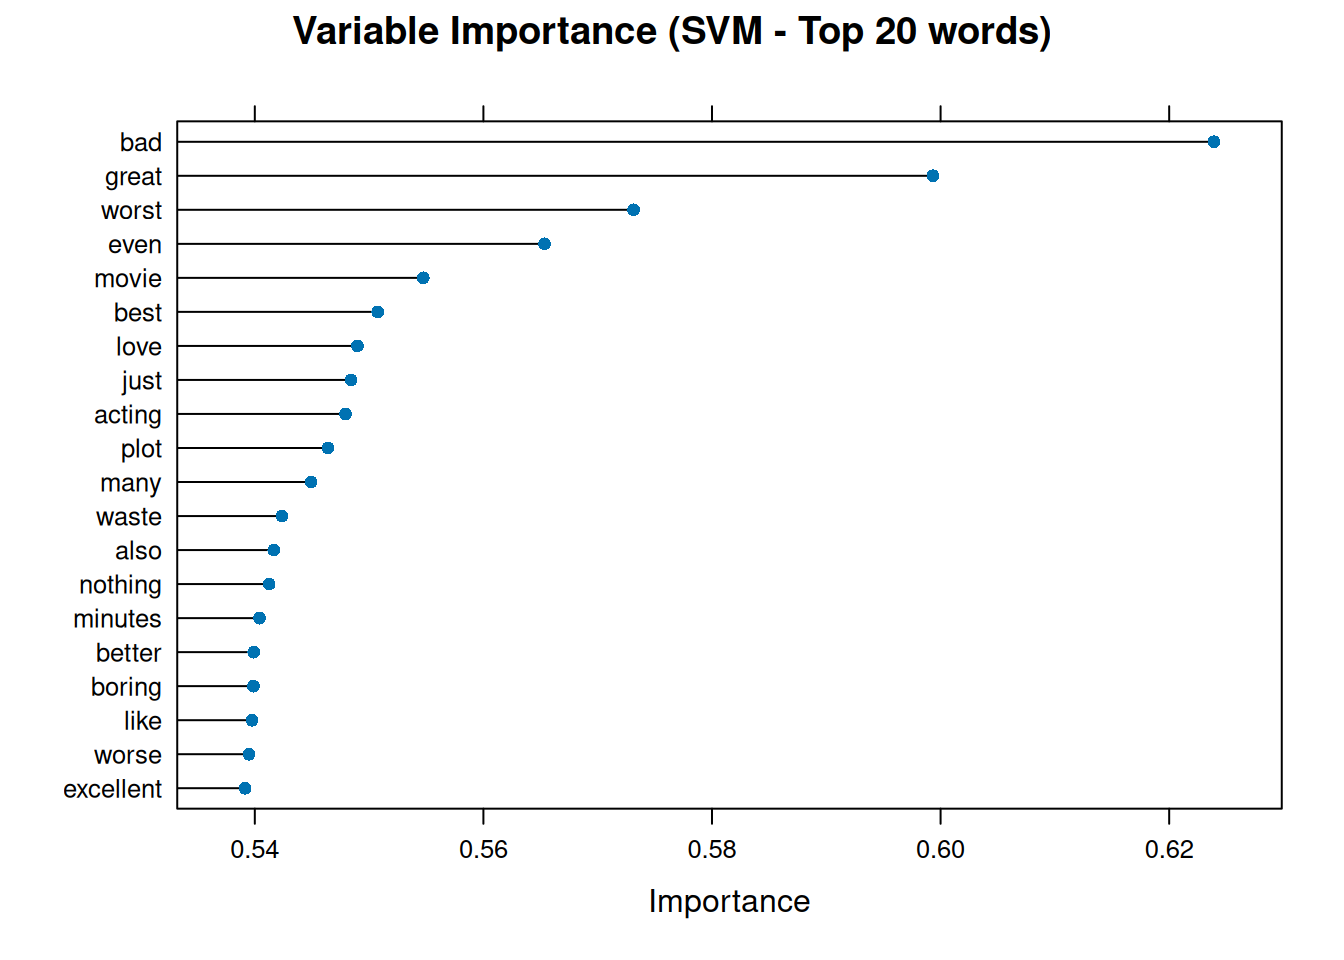
\includegraphics[keepaspectratio]{Introduction-to-Quantitative-Text-Analysis_files/figure-latex/svm-polarity-variable-importance-1.pdf}}

This graph illustrates the words that greatly influenced the SVM model's polarity classification decisions. Words with high importance may have large positive or negative coefficients, which push documents towards the `pos' or `neg' class boundary.

Next, we plot the Receiver Operating Characteristic (ROC) curve using the predicted probabilities from the test set and the actual test labels and calculate the Area Under the Curve (AUC). The ROC curve illustrates the trade-off between sensitivity and specificity as the classification threshold varies.

The ROC curve is another common way to evaluate binary classifiers. It plots the true positive rate (sensitivity) against the false positive rate (1 - specificity) at various classification threshold settings. A model that performs no better than random guessing would have a ROC curve close to the diagonal line (from bottom-left to top-right). A good model will have an ROC curve that bows towards the top-left corner. The area under the curve (AUC) summarises the ROC curve into a single number. An AUC of 1 indicates a perfect classifier; an AUC of 0.5 indicates performance no better than random chance; and an AUC of less than 0.5 suggests performance worse than random chance, indicating something is likely wrong, such as the flipped labels.

\begin{Shaded}
\begin{Highlighting}[]
\CommentTok{\# The roc() function needs the actual responses (factor) and the predicted}
\CommentTok{\# probabilities for the positive class (numeric)}
\NormalTok{roc\_obj\_svm }\OtherTok{\textless{}{-}} \FunctionTok{roc}\NormalTok{(}\AttributeTok{response =}\NormalTok{ polarity\_test, }\AttributeTok{predictor =}\NormalTok{ svm\_predict\_probs\_caret\_cv[,}
    \StringTok{"pos"}\NormalTok{], }\AttributeTok{levels =} \FunctionTok{levels}\NormalTok{(polarity\_test))}
\FunctionTok{plot}\NormalTok{(roc\_obj\_svm, }\AttributeTok{main =} \StringTok{"ROC Curve (SVM Test Set)"}\NormalTok{, }\AttributeTok{legacy.axes =} \ConstantTok{TRUE}\NormalTok{)}

\NormalTok{auc\_value\_svm }\OtherTok{\textless{}{-}} \FunctionTok{auc}\NormalTok{(roc\_obj\_svm)  }\CommentTok{\# Add AUC value to the plot}
\FunctionTok{legend}\NormalTok{(}\StringTok{"bottomright"}\NormalTok{, }\AttributeTok{legend =} \FunctionTok{paste}\NormalTok{(}\StringTok{"AUC ="}\NormalTok{, }\FunctionTok{round}\NormalTok{(auc\_value\_svm, }\DecValTok{3}\NormalTok{)), }\AttributeTok{bty =} \StringTok{"n"}\NormalTok{)}
\end{Highlighting}
\end{Shaded}

\pandocbounded{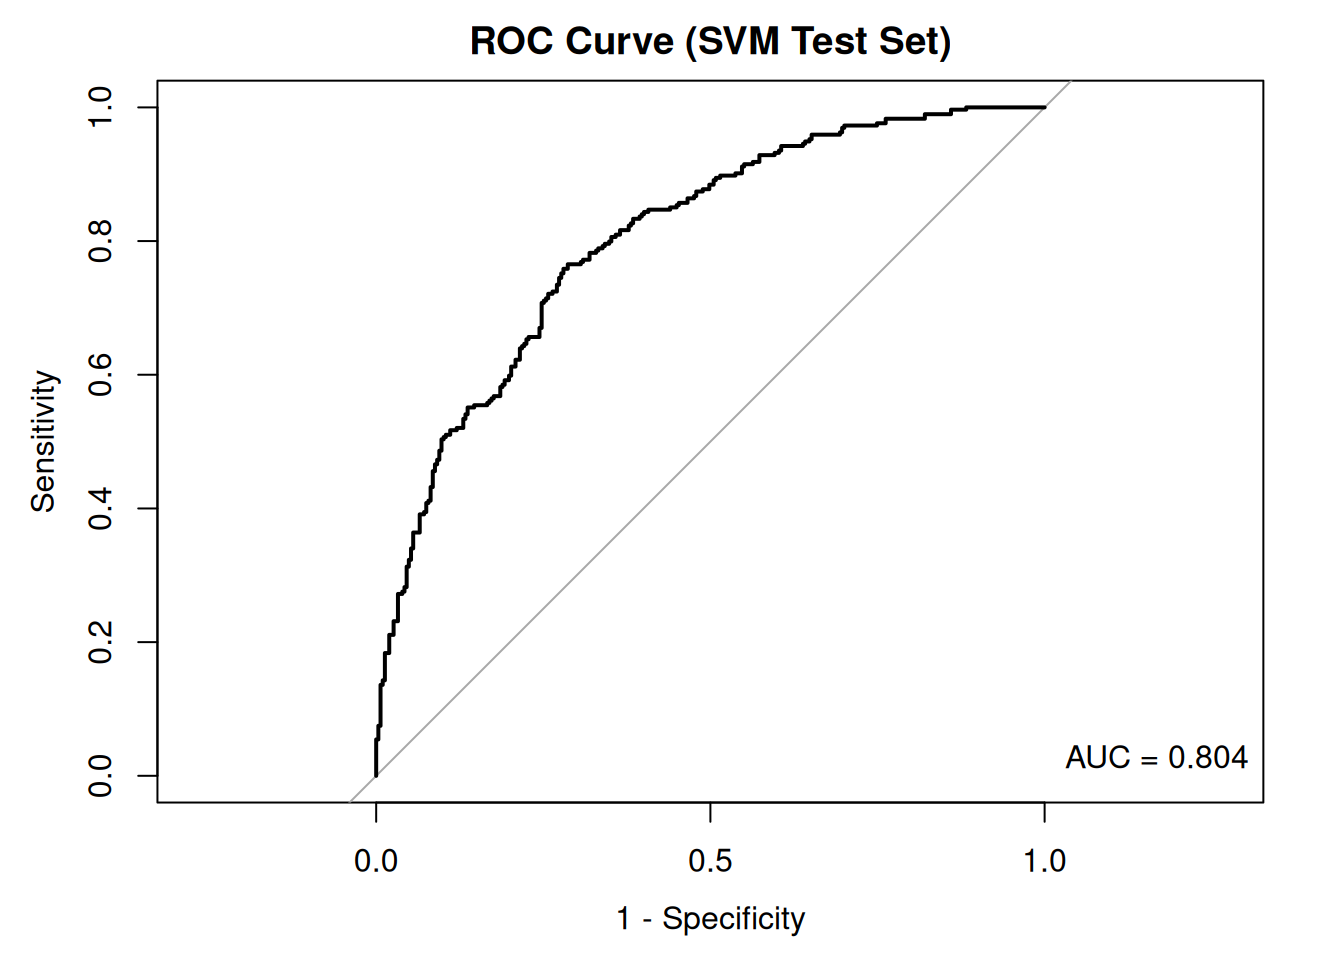
\includegraphics[keepaspectratio]{Introduction-to-Quantitative-Text-Analysis_files/figure-latex/svm-polarity-roc-1.pdf}}

The ROC curve and the area under the curve (AUC) provide insight into the model's ability to distinguish between positive and negative classes. An AUC close to 1 indicates excellent discrimination, whereas an AUC close to 0.5 suggests that the model performs no better than by chance.

Finally, we can examine the calibration plot. This shows how well the predicted probabilities match the observed frequencies in the test set. In a well-calibrated model, the points should lie close to the diagonal line. This indicates that a predicted probability of 0.8, for example, corresponds to the positive class occurring in approximately 80\% of instances with that predicted probability. A calibration plot helps us to assess whether the model's predicted probabilities are reliable. For example, suppose the model predicts a probability of 0.8 for a set of reviews being `positive'. In that case, we hope about 80\% of those reviews are positive---the plot groups predictions by probability score. For example, it groups all reviews where P(positive) is between 0.7 and 0.8 and plots the proportion of positive reviews observed in each group against the predicted probability. A perfectly calibrated model would have points along the diagonal line (y = x).

\begin{Shaded}
\begin{Highlighting}[]
\CommentTok{\# Create a data frame containing the observed outcomes and the predicted probabilities}

\NormalTok{calibration\_data }\OtherTok{\textless{}{-}} \FunctionTok{data.frame}\NormalTok{(}\AttributeTok{obs =}\NormalTok{ polarity\_test, }\AttributeTok{prob\_pos =}\NormalTok{ svm\_predict\_probs\_caret\_cv[, }\StringTok{"pos"}\NormalTok{])}

\CommentTok{\# Compute calibration information}

\NormalTok{calibration\_obj\_svm }\OtherTok{\textless{}{-}} \FunctionTok{calibration}\NormalTok{(}
\NormalTok{  obs }\SpecialCharTok{\textasciitilde{}}\NormalTok{ prob\_pos,}
  \CommentTok{\# Formula: observed variable \textasciitilde{} predicted probability variable}
  \AttributeTok{data =}\NormalTok{ calibration\_data,}
  \CommentTok{\# The data frame containing these variables}
  \AttributeTok{class =} \StringTok{"pos"}\NormalTok{,}
  \CommentTok{\# Specify the positive class name from the \textquotesingle{}obs\textquotesingle{} column}
  \AttributeTok{cuts =} \DecValTok{10}\NormalTok{,}
  \CommentTok{\# Number of bins (quantiles) for grouping probabilities}
  \AttributeTok{method =} \StringTok{"quantile"} \CommentTok{\# Method for creating bins}
\NormalTok{)}

\NormalTok{calibration\_data\_for\_plot }\OtherTok{\textless{}{-}}\NormalTok{ calibration\_obj\_svm}\SpecialCharTok{$}\NormalTok{data}

\FunctionTok{ggplot}\NormalTok{(}\AttributeTok{data =}\NormalTok{ calibration\_data\_for\_plot, }\FunctionTok{aes}\NormalTok{(}\AttributeTok{x =}\NormalTok{ midpoint, }\AttributeTok{y =}\NormalTok{ Percent)) }\SpecialCharTok{+}
  \FunctionTok{geom\_line}\NormalTok{() }\SpecialCharTok{+} \CommentTok{\# Plot the calibration line connecting the points}
  \FunctionTok{geom\_point}\NormalTok{() }\SpecialCharTok{+} \CommentTok{\# Plot the points for each bin}
  \FunctionTok{geom\_abline}\NormalTok{(}
    \AttributeTok{intercept =} \DecValTok{0}\NormalTok{,}
    \AttributeTok{slope =} \DecValTok{1}\NormalTok{,}
    \AttributeTok{linetype =} \StringTok{"dashed"}\NormalTok{,}
    \AttributeTok{color =} \StringTok{"darkred"}
\NormalTok{  ) }\SpecialCharTok{+}
  \FunctionTok{scale\_x\_continuous}\NormalTok{(}\AttributeTok{name =} \StringTok{"Bin Midpoint"}\NormalTok{, }\AttributeTok{limits =} \FunctionTok{c}\NormalTok{(}\DecValTok{0}\NormalTok{, }\DecValTok{100}\NormalTok{)) }\SpecialCharTok{+}
  \FunctionTok{scale\_y\_continuous}\NormalTok{(}\AttributeTok{name =} \StringTok{"Observed Event Percentage"}\NormalTok{, }\AttributeTok{limits =} \FunctionTok{c}\NormalTok{(}\DecValTok{0}\NormalTok{, }\DecValTok{100}\NormalTok{)) }\SpecialCharTok{+}
  \FunctionTok{ggtitle}\NormalTok{(}\StringTok{"Calibration Plot"}\NormalTok{) }\SpecialCharTok{+}
  \FunctionTok{theme\_bw}\NormalTok{() }\SpecialCharTok{+}
  \FunctionTok{coord\_equal}\NormalTok{()}
\end{Highlighting}
\end{Shaded}

\pandocbounded{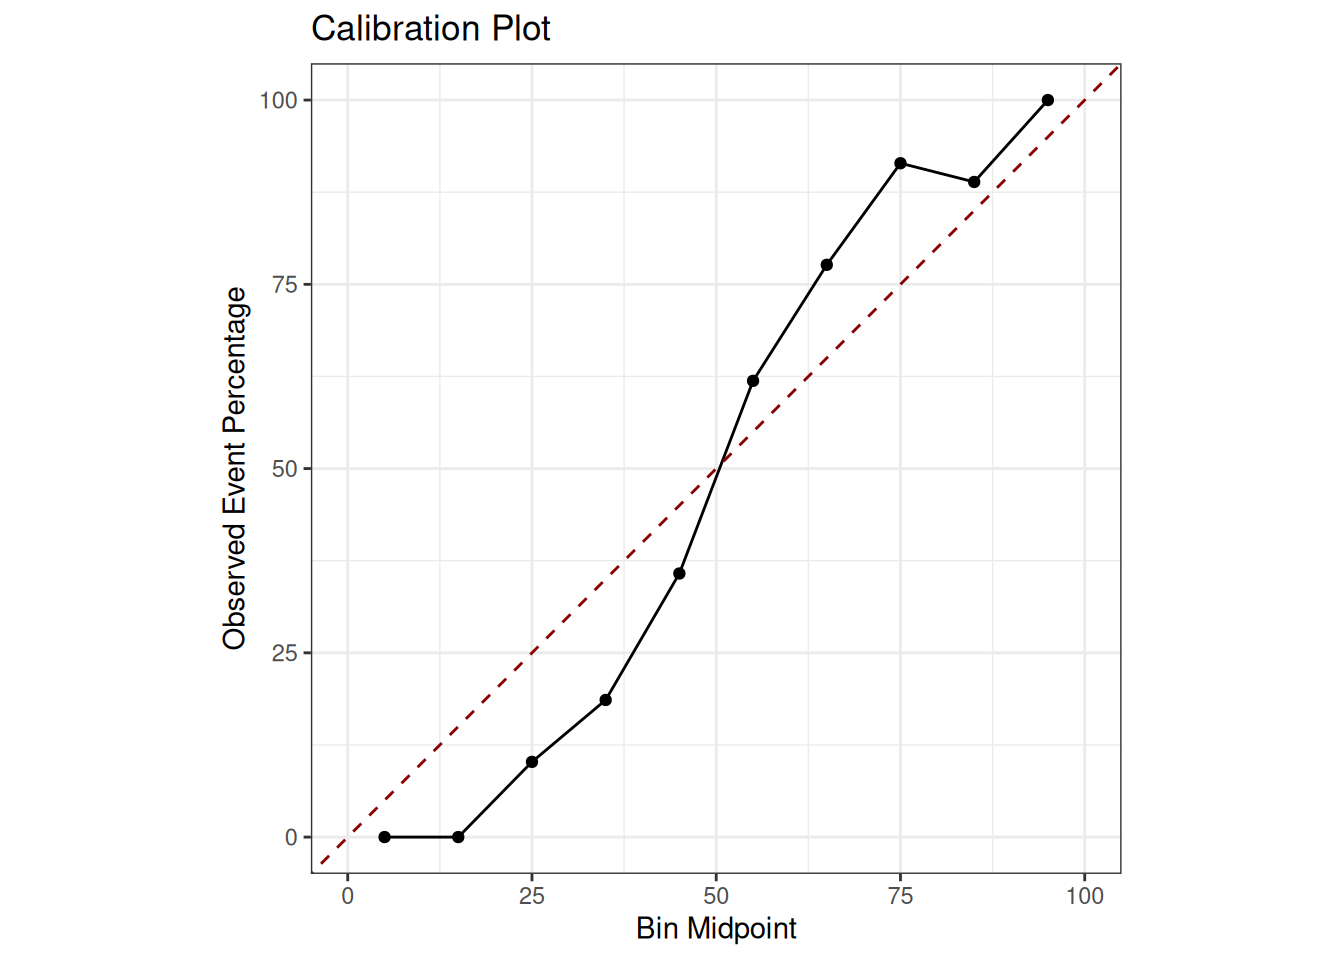
\includegraphics[keepaspectratio]{Introduction-to-Quantitative-Text-Analysis_files/figure-latex/svm-polarity-calibration-1.pdf}}

The closer the black line representing the model's calibration is to the red dashed line representing perfect calibration, the more reliable the model's probabilities are. Deviations from this indicate either overconfidence, where the line is above the diagonal for low probabilities and below it for high probabilities or underconfidence. Poor calibration means that, while the model may make the correct classification, the stated confidence level (i.e.~the probability) may be unreliable.

\section{Logistic Regression}\label{logistic-regression}

Logistic Regression is one of the most well-known types of supervised models and is well-suited for classification because \texttt{textmodel\_lr} is already built-in, it is practical to use in R. In addition, this implementation includes L2 regularisation by default to prevent overfitting in high-dimensional text feature spaces. For consistency, we will reuse the data loading, sampling, splitting, and preprocessing steps from the SVM example.

First, ensure the necessary libraries are loaded:

\begin{Shaded}
\begin{Highlighting}[]
\FunctionTok{set.seed}\NormalTok{(}\DecValTok{42}\NormalTok{)  }\CommentTok{\# Set seed for reproducibility}

\FunctionTok{library}\NormalTok{(quanteda)}
\FunctionTok{library}\NormalTok{(quanteda.textmodels)  }\CommentTok{\# For textmodel\_lr}
\FunctionTok{library}\NormalTok{(caret)  }\CommentTok{\# For evaluation metrics}
\FunctionTok{library}\NormalTok{(pROC)  }\CommentTok{\# For ROC analysis (optional, but good for binary classification)}
\FunctionTok{library}\NormalTok{(ggplot2)  }\CommentTok{\# For plotting (optional)}

\CommentTok{\# Load the movie review corpus and sample a subset (matching the SVM example)}
\NormalTok{corpus\_reviews\_lr }\OtherTok{\textless{}{-}} \FunctionTok{corpus\_sample}\NormalTok{(data\_corpus\_LMRD, }\DecValTok{2000}\NormalTok{)  }\CommentTok{\# Sample 2000 reviews}
\end{Highlighting}
\end{Shaded}

We will use the same data splitting logic as in the SVM example, ensuring a stratified split based on the \texttt{polarity} variable to maintain the proportion of positive and negative reviews in both the training and test sets.

\begin{Shaded}
\begin{Highlighting}[]
\CommentTok{\# Extract the polarity label as the target variable and convert it to a factor}
\CommentTok{\# Assuming the polarity variable is binary (\textquotesingle{}neg\textquotesingle{}, \textquotesingle{}pos\textquotesingle{}) in your corpus object}
\NormalTok{polarity\_labels\_lr }\OtherTok{\textless{}{-}} \FunctionTok{factor}\NormalTok{(corpus\_reviews\_lr}\SpecialCharTok{$}\NormalTok{polarity)}

\CommentTok{\# Identify documents with valid polarity labels (not NA)}
\NormalTok{valid\_docs\_index\_lr }\OtherTok{\textless{}{-}} \FunctionTok{which}\NormalTok{(}\SpecialCharTok{!}\FunctionTok{is.na}\NormalTok{(polarity\_labels\_lr))}

\CommentTok{\# Subset the corpus and polarity labels to only include documents with valid}
\CommentTok{\# polarity}
\NormalTok{corpus\_reviews\_valid\_lr }\OtherTok{\textless{}{-}}\NormalTok{ corpus\_reviews\_lr[valid\_docs\_index\_lr]}
\NormalTok{polarity\_valid\_lr }\OtherTok{\textless{}{-}}\NormalTok{ polarity\_labels\_lr[valid\_docs\_index\_lr]}

\CommentTok{\# Ensure polarity\_valid\_lr is a factor with levels \textquotesingle{}neg\textquotesingle{}, \textquotesingle{}pos\textquotesingle{} in that}
\CommentTok{\# specific order}
\NormalTok{polarity\_valid\_lr }\OtherTok{\textless{}{-}} \FunctionTok{factor}\NormalTok{(polarity\_valid\_lr, }\AttributeTok{levels =} \FunctionTok{c}\NormalTok{(}\StringTok{"neg"}\NormalTok{, }\StringTok{"pos"}\NormalTok{))}

\CommentTok{\# Check if both levels (\textquotesingle{}neg\textquotesingle{}, \textquotesingle{}pos\textquotesingle{}) are present}
\ControlFlowTok{if}\NormalTok{ (}\SpecialCharTok{!}\FunctionTok{all}\NormalTok{(}\FunctionTok{c}\NormalTok{(}\StringTok{"neg"}\NormalTok{, }\StringTok{"pos"}\NormalTok{) }\SpecialCharTok{\%in\%} \FunctionTok{levels}\NormalTok{(polarity\_valid\_lr)) }\SpecialCharTok{||} \FunctionTok{any}\NormalTok{(}\FunctionTok{table}\NormalTok{(polarity\_valid\_lr) }\SpecialCharTok{==}
    \DecValTok{0}\NormalTok{)) \{}
    \FunctionTok{stop}\NormalTok{(}\StringTok{"The sampled corpus subset does not contain both \textquotesingle{}neg\textquotesingle{} and \textquotesingle{}pos\textquotesingle{} classes after filtering NA polarity. Please increase the sample size or check data."}\NormalTok{)}
\NormalTok{\}}

\CommentTok{\# Manually create stratified split indices (reusing the logic from the SVM}
\CommentTok{\# example) Get indices for each class}
\NormalTok{neg\_indices\_lr }\OtherTok{\textless{}{-}} \FunctionTok{which}\NormalTok{(polarity\_valid\_lr }\SpecialCharTok{==} \StringTok{"neg"}\NormalTok{)}
\NormalTok{pos\_indices\_lr }\OtherTok{\textless{}{-}} \FunctionTok{which}\NormalTok{(polarity\_valid\_lr }\SpecialCharTok{==} \StringTok{"pos"}\NormalTok{)}

\CommentTok{\# Determine the number of instances for train/test per class (70/30 split)}
\FunctionTok{set.seed}\NormalTok{(}\DecValTok{42}\NormalTok{)  }\CommentTok{\# for reproducibility}
\NormalTok{train\_size\_neg\_lr }\OtherTok{\textless{}{-}} \FunctionTok{floor}\NormalTok{(}\FloatTok{0.7} \SpecialCharTok{*} \FunctionTok{length}\NormalTok{(neg\_indices\_lr))}
\NormalTok{train\_size\_pos\_lr }\OtherTok{\textless{}{-}} \FunctionTok{floor}\NormalTok{(}\FloatTok{0.7} \SpecialCharTok{*} \FunctionTok{length}\NormalTok{(pos\_indices\_lr))}

\CommentTok{\# Sample indices for training set from each class}
\NormalTok{train\_indices\_neg\_lr }\OtherTok{\textless{}{-}} \FunctionTok{sample}\NormalTok{(neg\_indices\_lr, }\AttributeTok{size =}\NormalTok{ train\_size\_neg\_lr, }\AttributeTok{replace =} \ConstantTok{FALSE}\NormalTok{)}
\NormalTok{train\_indices\_pos\_lr }\OtherTok{\textless{}{-}} \FunctionTok{sample}\NormalTok{(pos\_indices\_lr, }\AttributeTok{size =}\NormalTok{ train\_size\_pos\_lr, }\AttributeTok{replace =} \ConstantTok{FALSE}\NormalTok{)}

\CommentTok{\# Combine training indices}
\NormalTok{train\_index\_lr }\OtherTok{\textless{}{-}} \FunctionTok{c}\NormalTok{(train\_indices\_neg\_lr, train\_indices\_pos\_lr)}

\CommentTok{\# The remaining indices are for the test set}
\NormalTok{all\_valid\_indices\_lr }\OtherTok{\textless{}{-}} \FunctionTok{seq\_along}\NormalTok{(polarity\_valid\_lr)}
\NormalTok{test\_index\_lr }\OtherTok{\textless{}{-}}\NormalTok{ all\_valid\_indices\_lr[}\SpecialCharTok{!}\NormalTok{all\_valid\_indices\_lr }\SpecialCharTok{\%in\%}\NormalTok{ train\_index\_lr]}

\CommentTok{\# Split the corpus subset and polarity labels into training and testing sets}
\NormalTok{corpus\_reviews\_train\_lr }\OtherTok{\textless{}{-}}\NormalTok{ corpus\_reviews\_valid\_lr[train\_index\_lr]}
\NormalTok{corpus\_reviews\_test\_lr }\OtherTok{\textless{}{-}}\NormalTok{ corpus\_reviews\_valid\_lr[test\_index\_lr]}

\NormalTok{polarity\_train\_lr }\OtherTok{\textless{}{-}}\NormalTok{ polarity\_valid\_lr[train\_index\_lr]}
\NormalTok{polarity\_test\_lr }\OtherTok{\textless{}{-}}\NormalTok{ polarity\_valid\_lr[test\_index\_lr]}

\CommentTok{\# Check the distribution of the split}
\FunctionTok{print}\NormalTok{(}\StringTok{"Training set class distribution (LR example):"}\NormalTok{)}
\end{Highlighting}
\end{Shaded}

\begin{verbatim}
## [1] "Training set class distribution (LR example):"
\end{verbatim}

\begin{Shaded}
\begin{Highlighting}[]
\FunctionTok{print}\NormalTok{(}\FunctionTok{table}\NormalTok{(polarity\_train\_lr))}
\end{Highlighting}
\end{Shaded}

\begin{verbatim}
## polarity_train_lr
## neg pos 
## 716 683
\end{verbatim}

\begin{Shaded}
\begin{Highlighting}[]
\FunctionTok{print}\NormalTok{(}\StringTok{"Testing set class distribution (LR example):"}\NormalTok{)}
\end{Highlighting}
\end{Shaded}

\begin{verbatim}
## [1] "Testing set class distribution (LR example):"
\end{verbatim}

\begin{Shaded}
\begin{Highlighting}[]
\FunctionTok{print}\NormalTok{(}\FunctionTok{table}\NormalTok{(polarity\_test\_lr))}
\end{Highlighting}
\end{Shaded}

\begin{verbatim}
## polarity_test_lr
## neg pos 
## 307 294
\end{verbatim}

Next, we preprocess the training and test corpus subsets to create DFMs, applying similar cleaning steps as before and matching the test DFM features to the training DFM.

\begin{Shaded}
\begin{Highlighting}[]
\CommentTok{\# Tokenise and preprocess the training corpus}
\NormalTok{tokens\_train\_lr }\OtherTok{\textless{}{-}} \FunctionTok{tokens}\NormalTok{(corpus\_reviews\_train\_lr, }\AttributeTok{what =} \StringTok{"word"}\NormalTok{, }\AttributeTok{remove\_punct =} \ConstantTok{TRUE}\NormalTok{,}
    \AttributeTok{remove\_symbols =} \ConstantTok{TRUE}\NormalTok{, }\AttributeTok{remove\_numbers =} \ConstantTok{TRUE}\NormalTok{, }\AttributeTok{remove\_url =} \ConstantTok{TRUE}\NormalTok{, }\AttributeTok{remove\_separators =} \ConstantTok{TRUE}\NormalTok{) }\SpecialCharTok{\%\textgreater{}\%}
    \FunctionTok{tokens\_tolower}\NormalTok{() }\SpecialCharTok{\%\textgreater{}\%}
    \FunctionTok{tokens\_select}\NormalTok{(}\FunctionTok{stopwords}\NormalTok{(}\StringTok{"english"}\NormalTok{), }\AttributeTok{selection =} \StringTok{"remove"}\NormalTok{)}

\CommentTok{\# Tokenise and preprocess the test corpus}
\NormalTok{tokens\_test\_lr }\OtherTok{\textless{}{-}} \FunctionTok{tokens}\NormalTok{(corpus\_reviews\_test\_lr, }\AttributeTok{what =} \StringTok{"word"}\NormalTok{, }\AttributeTok{remove\_punct =} \ConstantTok{TRUE}\NormalTok{,}
    \AttributeTok{remove\_symbols =} \ConstantTok{TRUE}\NormalTok{, }\AttributeTok{remove\_numbers =} \ConstantTok{TRUE}\NormalTok{, }\AttributeTok{remove\_url =} \ConstantTok{TRUE}\NormalTok{, }\AttributeTok{remove\_separators =} \ConstantTok{TRUE}\NormalTok{) }\SpecialCharTok{\%\textgreater{}\%}
    \FunctionTok{tokens\_tolower}\NormalTok{() }\SpecialCharTok{\%\textgreater{}\%}
    \FunctionTok{tokens\_select}\NormalTok{(}\FunctionTok{stopwords}\NormalTok{(}\StringTok{"english"}\NormalTok{), }\AttributeTok{selection =} \StringTok{"remove"}\NormalTok{)}

\CommentTok{\# Create dfms}
\NormalTok{dfm\_train\_lr }\OtherTok{\textless{}{-}} \FunctionTok{dfm}\NormalTok{(tokens\_train\_lr)}
\NormalTok{dfm\_test\_lr }\OtherTok{\textless{}{-}} \FunctionTok{dfm}\NormalTok{(tokens\_test\_lr)}

\CommentTok{\# Ensure the test dfm has the same features as the training dfm}
\NormalTok{dfm\_test\_matched\_lr }\OtherTok{\textless{}{-}} \FunctionTok{dfm\_match}\NormalTok{(dfm\_test\_lr, }\AttributeTok{features =} \FunctionTok{featnames}\NormalTok{(dfm\_train\_lr))}

\CommentTok{\# Display DFM dimensions}
\FunctionTok{cat}\NormalTok{(}\StringTok{"Dimensions of Training DFM (LR example):"}\NormalTok{, }\FunctionTok{dim}\NormalTok{(dfm\_train\_lr), }\StringTok{"}\SpecialCharTok{\textbackslash{}n}\StringTok{"}\NormalTok{)}
\end{Highlighting}
\end{Shaded}

\begin{verbatim}
## Dimensions of Training DFM (LR example): 1399 23543
\end{verbatim}

\begin{Shaded}
\begin{Highlighting}[]
\FunctionTok{cat}\NormalTok{(}\StringTok{"Dimensions of Matched Test DFM (LR example):"}\NormalTok{, }\FunctionTok{dim}\NormalTok{(dfm\_test\_matched\_lr), }\StringTok{"}\SpecialCharTok{\textbackslash{}n}\StringTok{"}\NormalTok{)}
\end{Highlighting}
\end{Shaded}

\begin{verbatim}
## Dimensions of Matched Test DFM (LR example): 601 23543
\end{verbatim}

Now, we train the Regularized Logistic Regression model using \texttt{textmodel\_lr}.

\begin{Shaded}
\begin{Highlighting}[]
\CommentTok{\# Train the textmodel\_lr model for binary classification The training labels}
\CommentTok{\# are the polarity labels from the training corpus}
\FunctionTok{library}\NormalTok{(quanteda.textmodels)}

\NormalTok{model\_lr\_lmrd }\OtherTok{\textless{}{-}} \FunctionTok{textmodel\_lr}\NormalTok{(dfm\_train\_lr, polarity\_train\_lr)}

\CommentTok{\# Print the model summary}
\FunctionTok{summary}\NormalTok{(model\_lr\_lmrd)}
\end{Highlighting}
\end{Shaded}

\begin{verbatim}
## 
## Call:
## textmodel_lr.dfm(x = dfm_train_lr, y = polarity_train_lr)
## 
## Lambda Min:
## [1] 0.009405
## 
## Lambda 1se:
## [1] 0.01498
## 
## Estimated Feature Scores:
##     (Intercept) just thought finish whole year without giving single movie bomb
## pos      0.1042    0       0      0     0    0       0      0      0     0    0
##     rating friend brought notorious turd house last night feared  worst knowing
## pos      0      0       0         0    0     0    0     0      0 -1.281       0
##     reputation god-awful anticipated mexican-made mess dubbed english produced
## pos          0         0           0            0    0      0       0        0
\end{verbatim}

We then use the trained model to predict the polarity labels for the documents in the test set.

\begin{Shaded}
\begin{Highlighting}[]
\CommentTok{\# Predict the classes for the matched test set}
\NormalTok{predictions\_lr\_lmrd }\OtherTok{\textless{}{-}} \FunctionTok{predict}\NormalTok{(model\_lr\_lmrd, }\AttributeTok{newdata =}\NormalTok{ dfm\_test\_matched\_lr)}

\CommentTok{\# Display the first few predictions}
\FunctionTok{head}\NormalTok{(predictions\_lr\_lmrd)}
\end{Highlighting}
\end{Shaded}

\begin{verbatim}
##  test/neg/6932_2.txt train/neg/6580_4.txt  test/pos/1099_7.txt 
##                  neg                  pos                  pos 
## train/pos/9167_7.txt  test/neg/8064_1.txt  test/neg/4057_4.txt 
##                  neg                  neg                  pos 
## Levels: neg pos
\end{verbatim}

Finally, we evaluate the model's performance on the test set using a confusion matrix. Since this is a binary classification task, we can also compute metrics like ROC AUC, which is similar to the SVM evaluation.

\begin{Shaded}
\begin{Highlighting}[]
\CommentTok{\# Get the actual classes from the test corpus}
\NormalTok{actual\_classes\_lmrd }\OtherTok{\textless{}{-}}\NormalTok{ polarity\_test\_lr}

\CommentTok{\# Ensure actual and predicted classes are factors with the same levels for}
\CommentTok{\# comparison The levels should already be consistent (\textquotesingle{}neg\textquotesingle{}, \textquotesingle{}pos\textquotesingle{}) from the}
\CommentTok{\# splitting step}
\NormalTok{confusion\_matrix\_lr\_lmrd }\OtherTok{\textless{}{-}} \FunctionTok{confusionMatrix}\NormalTok{(predictions\_lr\_lmrd, actual\_classes\_lmrd)}

\CommentTok{\# Print the confusion matrix and performance statistics}
\FunctionTok{print}\NormalTok{(confusion\_matrix\_lr\_lmrd)}
\end{Highlighting}
\end{Shaded}

\begin{verbatim}
## Confusion Matrix and Statistics
## 
##           Reference
## Prediction neg pos
##        neg 232  46
##        pos  75 248
##                                         
##                Accuracy : 0.7987        
##                  95% CI : (0.7643, 0.83)
##     No Information Rate : 0.5108        
##     P-Value [Acc > NIR] : < 2e-16       
##                                         
##                   Kappa : 0.598         
##                                         
##  Mcnemar's Test P-Value : 0.01091       
##                                         
##             Sensitivity : 0.7557        
##             Specificity : 0.8435        
##          Pos Pred Value : 0.8345        
##          Neg Pred Value : 0.7678        
##              Prevalence : 0.5108        
##          Detection Rate : 0.3860        
##    Detection Prevalence : 0.4626        
##       Balanced Accuracy : 0.7996        
##                                         
##        'Positive' Class : neg           
## 
\end{verbatim}

\section{Naive Bayes (NB)}\label{naive-bayes-nb}

As with SVM, Naive Bayes is a simple yet efficient text classification model. It belongs to a family of probabilistic classifiers based on applying Bayes' Theorem with a ``naive'' that every word in a document is conditionally independent of every other word given the class. The classifier calculates this value for each class and assigns the document to the class with the highest resulting probability. Despite its simplifying assumption, Naive Bayes performs remarkably well for many text classification tasks, such as spam detection and document categorization.

For this example, we will use data from the \href{https://manifestoproject.wzb.eu/}{Manifesto Project} (also known as the Comparative Manifesto Project (CMP)). To use this data, ensure you have signed up, downloaded the API key, loaded the package, and set the key.

\begin{Shaded}
\begin{Highlighting}[]
\FunctionTok{library}\NormalTok{(manifestoR)  }\CommentTok{\# Used to download Manifesto Project data}
\FunctionTok{library}\NormalTok{(quanteda)  }\CommentTok{\# For text analysis and DFM creation}
\FunctionTok{library}\NormalTok{(quanteda.textmodels)  }\CommentTok{\# For the Naive Bayes model}
\FunctionTok{library}\NormalTok{(ggplot2)  }\CommentTok{\# For plotting}
\FunctionTok{library}\NormalTok{(DescTools)  }\CommentTok{\# For Krippendorf\textquotesingle{}s Alpha}
\FunctionTok{library}\NormalTok{(caret)  }\CommentTok{\# For confusion matrix and classification metrics}
\FunctionTok{library}\NormalTok{(dplyr)  }\CommentTok{\# For data manipulation}

\CommentTok{\# Set your Manifesto Project API key Replace \textquotesingle{}manifesto\_apikey.txt\textquotesingle{} with the}
\CommentTok{\# path to your API key file}
\FunctionTok{mp\_setapikey}\NormalTok{(}\StringTok{"manifesto\_apikey.txt"}\NormalTok{)}
\end{Highlighting}
\end{Shaded}

As the entire MP corpus is relatively large, here we will only focus on part of it: the manifestos for the 2015 United Kingdom general election. To achieve this, we have created a data frame listing the party and year for the `mp\_corpus' command. Please note that The Manifesto Project uses unique codes for each party, which can be found in its codebook.

\begin{Shaded}
\begin{Highlighting}[]
\CommentTok{\# Party codes: CON(51620), LABOUR(51320), LIBDEM(51421), SNP(51901), PLAID}
\CommentTok{\# CYMRU(51902), GREEN(51110), UKIP(51951)}
\NormalTok{manifestos\_info }\OtherTok{\textless{}{-}} \FunctionTok{data.frame}\NormalTok{(}\AttributeTok{party =} \FunctionTok{c}\NormalTok{(}\DecValTok{51320}\NormalTok{, }\DecValTok{51620}\NormalTok{, }\DecValTok{51110}\NormalTok{, }\DecValTok{51421}\NormalTok{, }\DecValTok{51901}\NormalTok{, }\DecValTok{51902}\NormalTok{,}
    \DecValTok{51951}\NormalTok{), }\AttributeTok{date =} \FunctionTok{rep}\NormalTok{(}\DecValTok{201505}\NormalTok{, }\DecValTok{7}\NormalTok{))}

\CommentTok{\# Download the specified manifestos as a manifestoR corpus}
\NormalTok{manifesto\_corpus }\OtherTok{\textless{}{-}} \FunctionTok{mp\_corpus}\NormalTok{(manifestos\_info)}
\end{Highlighting}
\end{Shaded}

\begin{verbatim}
## Connecting to Manifesto Project DB API... corpus version: 2024-1 
## Connecting to Manifesto Project DB API... corpus version: 2024-1
\end{verbatim}

We will create a data frame containing the quasi-sentences (the unit of analysis), their assigned \texttt{cmp\_code}, and the \texttt{party} they belong to. This process extracts the core data needed for our analysis.

\begin{Shaded}
\begin{Highlighting}[]
\CommentTok{\# Programmatically create a list of data frames, one for each document}
\NormalTok{corpus\_list }\OtherTok{\textless{}{-}} \FunctionTok{lapply}\NormalTok{(manifesto\_corpus, }\ControlFlowTok{function}\NormalTok{(doc) \{}
    \FunctionTok{data.frame}\NormalTok{(}\AttributeTok{texts =} \FunctionTok{content}\NormalTok{(doc), }\AttributeTok{cmp\_code =} \FunctionTok{codes}\NormalTok{(doc), }\AttributeTok{party =}\NormalTok{ doc}\SpecialCharTok{$}\NormalTok{meta}\SpecialCharTok{$}\NormalTok{party,}
        \AttributeTok{stringsAsFactors =} \ConstantTok{FALSE}\NormalTok{)}
\NormalTok{\})}

\CommentTok{\# Combine the list of data frames into a single data frame}
\NormalTok{manifesto\_data }\OtherTok{\textless{}{-}} \FunctionTok{do.call}\NormalTok{(rbind, corpus\_list)}
\end{Highlighting}
\end{Shaded}

Next, we clean and transform the data. We convert the \texttt{party} codes to factor labels (e.g., ``CON'', ``LABOUR'') for clarity, ensure text and code columns are in the correct format, and remove entries with \texttt{NA} codes, which typically correspond to un-coded document headers and titles.

\begin{Shaded}
\begin{Highlighting}[]
\CommentTok{\# Transform and clean the data frame}
\NormalTok{manifesto\_data}\SpecialCharTok{$}\NormalTok{party }\OtherTok{\textless{}{-}} \FunctionTok{factor}\NormalTok{(manifesto\_data}\SpecialCharTok{$}\NormalTok{party, }\AttributeTok{levels =} \FunctionTok{c}\NormalTok{(}\DecValTok{51110}\NormalTok{, }\DecValTok{51320}\NormalTok{, }\DecValTok{51421}\NormalTok{,}
    \DecValTok{51620}\NormalTok{, }\DecValTok{51901}\NormalTok{, }\DecValTok{51902}\NormalTok{, }\DecValTok{51951}\NormalTok{), }\AttributeTok{labels =} \FunctionTok{c}\NormalTok{(}\StringTok{"GREEN"}\NormalTok{, }\StringTok{"LABOUR"}\NormalTok{, }\StringTok{"LIBDEM"}\NormalTok{, }\StringTok{"CON"}\NormalTok{, }\StringTok{"PC"}\NormalTok{,}
    \StringTok{"SNP"}\NormalTok{, }\StringTok{"UKIP"}\NormalTok{))}
\NormalTok{manifesto\_data}\SpecialCharTok{$}\NormalTok{party }\OtherTok{\textless{}{-}} \FunctionTok{as.character}\NormalTok{(manifesto\_data}\SpecialCharTok{$}\NormalTok{party)}
\NormalTok{manifesto\_data}\SpecialCharTok{$}\NormalTok{texts }\OtherTok{\textless{}{-}} \FunctionTok{as.character}\NormalTok{(manifesto\_data}\SpecialCharTok{$}\NormalTok{texts)}
\NormalTok{manifesto\_data}\SpecialCharTok{$}\NormalTok{cmp\_code }\OtherTok{\textless{}{-}} \FunctionTok{as.numeric}\NormalTok{(}\FunctionTok{as.character}\NormalTok{(manifesto\_data}\SpecialCharTok{$}\NormalTok{cmp\_code))}

\CommentTok{\# Remove NA values (sentences without a code)}
\NormalTok{manifesto\_data }\OtherTok{\textless{}{-}} \FunctionTok{na.omit}\NormalTok{(manifesto\_data)}

\CommentTok{\# Display the structure of the cleaned data}
\FunctionTok{str}\NormalTok{(manifesto\_data)}
\end{Highlighting}
\end{Shaded}

\begin{verbatim}
## 'data.frame':    9763 obs. of  3 variables:
##  $ texts   : chr  "Our manifesto begins with the Budget Responsibility Lock we offer the British people." "It is the basis for all our plans in this manifesto because it is by securing our national finances that we are"| __truncated__ "Every policy in this manifesto is paid for." "Not one commitment requires additional borrowing." ...
##  $ cmp_code: num  414 414 414 414 414 414 414 414 414 414 ...
##  $ party   : chr  "LABOUR" "LABOUR" "LABOUR" "LABOUR" ...
##  - attr(*, "na.action")= 'omit' Named int [1:1014] 1 2 3 4 5 6 9 19 20 21 ...
##   ..- attr(*, "names")= chr [1:1014] "51320_201505.1" "51320_201505.2" "51320_201505.3" "51320_201505.4" ...
\end{verbatim}

We can calculate row percentages to understand how much a party ``owns'' a specific code. This shows the proportion of a code's total appearances attributed to each party.

\begin{Shaded}
\begin{Highlighting}[]
\CommentTok{\# Calculate row percentages of code occurrences by party}
\NormalTok{prop\_row }\OtherTok{\textless{}{-}} \FunctionTok{as.data.frame}\NormalTok{(}\FunctionTok{prop.table}\NormalTok{(}\FunctionTok{table}\NormalTok{(manifesto\_data}\SpecialCharTok{$}\NormalTok{cmp\_code, manifesto\_data}\SpecialCharTok{$}\NormalTok{party),}
    \AttributeTok{margin =} \DecValTok{1}\NormalTok{) }\SpecialCharTok{*} \DecValTok{100}\NormalTok{)}
\FunctionTok{names}\NormalTok{(prop\_row) }\OtherTok{\textless{}{-}} \FunctionTok{c}\NormalTok{(}\StringTok{"Code"}\NormalTok{, }\StringTok{"Party"}\NormalTok{, }\StringTok{"Percentage"}\NormalTok{)}

\CommentTok{\# Display head of row percentages}
\FunctionTok{head}\NormalTok{(prop\_row)}
\end{Highlighting}
\end{Shaded}

\begin{verbatim}
##   Code Party Percentage
## 1    0   CON   0.000000
## 2  101   CON  42.857143
## 3  103   CON 100.000000
## 4  104   CON  28.632479
## 5  105   CON   6.382979
## 6  106   CON   6.896552
\end{verbatim}

Visualizing the \texttt{prop\_row} object as a stacked bar chart clarifies how parties utilize different codes.

\begin{Shaded}
\begin{Highlighting}[]
\CommentTok{\# Define party colours for consistent plotting}
\NormalTok{party\_colors }\OtherTok{\textless{}{-}} \FunctionTok{c}\NormalTok{(}\AttributeTok{CON =} \StringTok{"\#0087DC"}\NormalTok{, }\AttributeTok{GREEN =} \StringTok{"\#67B437"}\NormalTok{, }\AttributeTok{LABOUR =} \StringTok{"\#DC241F"}\NormalTok{, }\AttributeTok{LIBDEM =} \StringTok{"\#FAA61A"}\NormalTok{,}
    \AttributeTok{PC =} \StringTok{"\#008142"}\NormalTok{, }\AttributeTok{SNP =} \StringTok{"\#FDF38E"}\NormalTok{, }\AttributeTok{UKIP =} \StringTok{"\#780077"}\NormalTok{)}

\CommentTok{\# Plot the row percentages}
\FunctionTok{ggplot}\NormalTok{(}\AttributeTok{data =}\NormalTok{ prop\_row, }\FunctionTok{aes}\NormalTok{(}\AttributeTok{x =} \FunctionTok{factor}\NormalTok{(Code), }\AttributeTok{y =}\NormalTok{ Percentage, }\AttributeTok{fill =}\NormalTok{ Party)) }\SpecialCharTok{+} \FunctionTok{scale\_fill\_manual}\NormalTok{(}\AttributeTok{values =}\NormalTok{ party\_colors) }\SpecialCharTok{+}
    \FunctionTok{geom\_bar}\NormalTok{(}\AttributeTok{stat =} \StringTok{"identity"}\NormalTok{, }\AttributeTok{position =} \StringTok{"stack"}\NormalTok{) }\SpecialCharTok{+} \FunctionTok{scale\_y\_continuous}\NormalTok{(}\AttributeTok{expand =} \FunctionTok{c}\NormalTok{(}\DecValTok{0}\NormalTok{,}
    \DecValTok{0}\NormalTok{)) }\SpecialCharTok{+} \FunctionTok{theme\_classic}\NormalTok{() }\SpecialCharTok{+} \FunctionTok{theme}\NormalTok{(}\AttributeTok{axis.text.x =} \FunctionTok{element\_text}\NormalTok{(}\AttributeTok{angle =} \DecValTok{90}\NormalTok{, }\AttributeTok{vjust =} \FloatTok{0.5}\NormalTok{,}
    \AttributeTok{size =} \DecValTok{8}\NormalTok{)) }\SpecialCharTok{+} \FunctionTok{labs}\NormalTok{(}\AttributeTok{x =} \StringTok{"Manifesto Code"}\NormalTok{, }\AttributeTok{y =} \StringTok{"Percentage of Code Occurrences"}\NormalTok{,}
    \AttributeTok{title =} \StringTok{"Party Ownership of Manifesto Codes (Row \%)"}\NormalTok{)}
\end{Highlighting}
\end{Shaded}

\pandocbounded{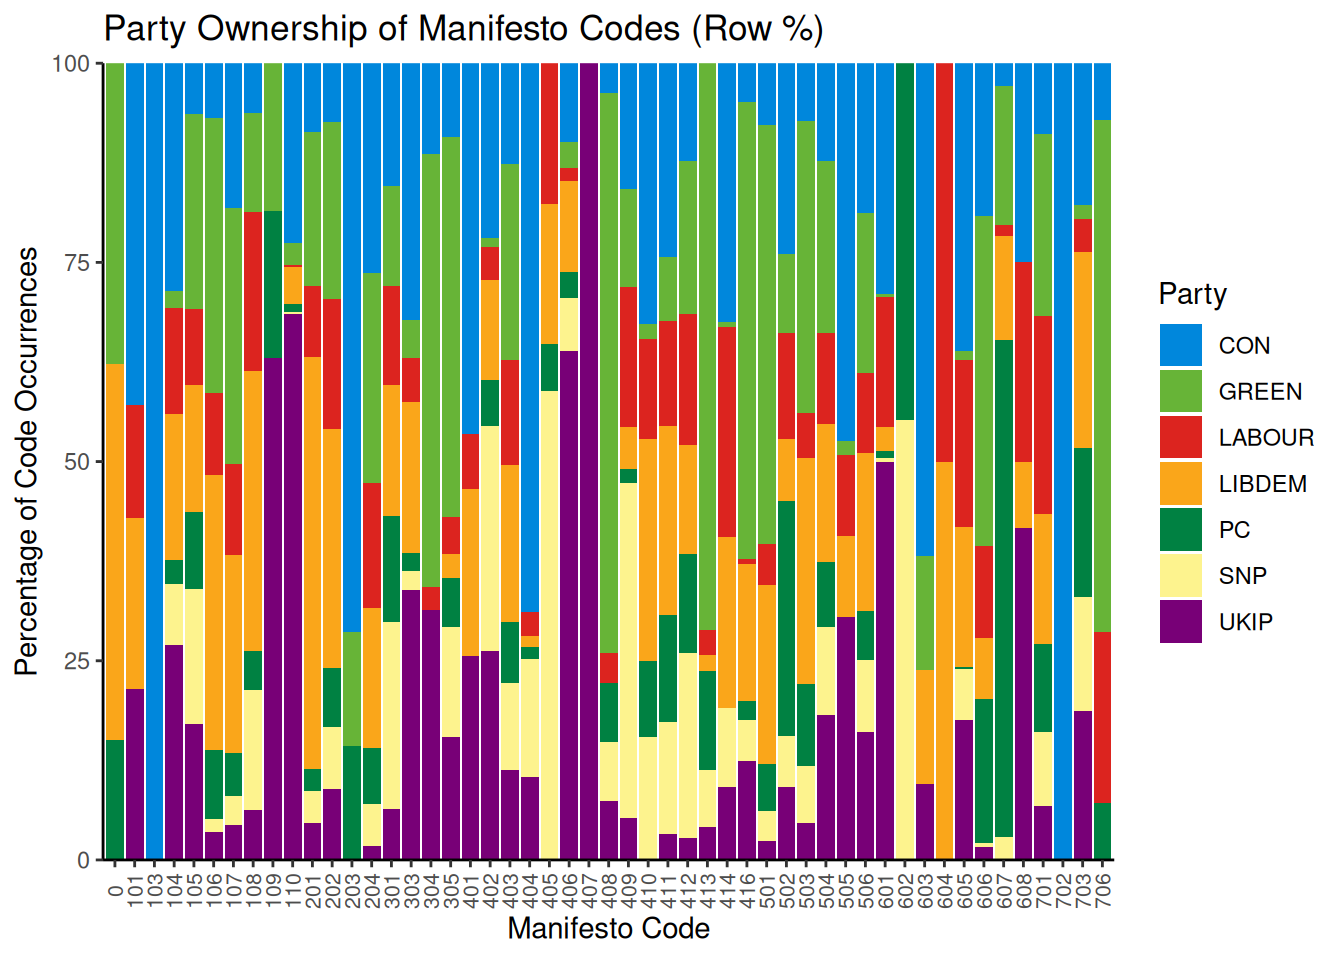
\includegraphics[keepaspectratio]{Introduction-to-Quantitative-Text-Analysis_files/figure-latex/ggplot-nb-codes-1.pdf}}

This chart shows that some parties dominate specific categories. For example, we can see that UKIP is the only one to use code 406 (Protectionism: Positive). Note that these are percentages; a high percentage might reflect dominance but could be based on a very small number of sentences. Other categories are more evenly distributed across parties. We can also analyze the thematic composition of each party's manifesto by calculating column percentages:

\begin{Shaded}
\begin{Highlighting}[]
\CommentTok{\# Calculate column percentages (percentage of party manifesto per code)}
\NormalTok{prop\_col }\OtherTok{\textless{}{-}} \FunctionTok{as.data.frame}\NormalTok{(}\FunctionTok{prop.table}\NormalTok{(}\FunctionTok{table}\NormalTok{(manifesto\_data}\SpecialCharTok{$}\NormalTok{cmp\_code, manifesto\_data}\SpecialCharTok{$}\NormalTok{party),}
    \AttributeTok{margin =} \DecValTok{2}\NormalTok{) }\SpecialCharTok{*} \DecValTok{100}\NormalTok{)}
\FunctionTok{names}\NormalTok{(prop\_col) }\OtherTok{\textless{}{-}} \FunctionTok{c}\NormalTok{(}\StringTok{"Code"}\NormalTok{, }\StringTok{"Party"}\NormalTok{, }\StringTok{"Percentage"}\NormalTok{)}

\CommentTok{\# Display head of column percentages}
\FunctionTok{head}\NormalTok{(prop\_col)}
\end{Highlighting}
\end{Shaded}

\begin{verbatim}
##   Code Party Percentage
## 1    0   CON  0.0000000
## 2  101   CON  0.3778338
## 3  103   CON  0.1259446
## 4  104   CON  4.2191436
## 5  105   CON  0.3778338
## 6  106   CON  0.2518892
\end{verbatim}

With 57 possible codes, grouping them into the 7 thematic domains defined by the Manifesto Project is more practical. We create a new \texttt{Domain} variable and assign each code to its corresponding domain.

\begin{Shaded}
\begin{Highlighting}[]
\CommentTok{\# Assign codes to their respective domains}
\NormalTok{prop\_col}\SpecialCharTok{$}\NormalTok{Code }\OtherTok{\textless{}{-}} \FunctionTok{as.numeric}\NormalTok{(}\FunctionTok{as.character}\NormalTok{(prop\_col}\SpecialCharTok{$}\NormalTok{Code))}
\NormalTok{prop\_col}\SpecialCharTok{$}\NormalTok{Domain }\OtherTok{\textless{}{-}} \FunctionTok{cut}\NormalTok{(prop\_col}\SpecialCharTok{$}\NormalTok{Code, }\AttributeTok{breaks =} \FunctionTok{c}\NormalTok{(}\SpecialCharTok{{-}}\DecValTok{1}\NormalTok{, }\DecValTok{0}\NormalTok{, }\DecValTok{110}\NormalTok{, }\DecValTok{204}\NormalTok{, }\DecValTok{305}\NormalTok{, }\DecValTok{416}\NormalTok{, }\DecValTok{507}\NormalTok{,}
    \DecValTok{608}\NormalTok{, }\DecValTok{706}\NormalTok{), }\AttributeTok{labels =} \FunctionTok{c}\NormalTok{(}\StringTok{"NA"}\NormalTok{, }\StringTok{"External Relations"}\NormalTok{, }\StringTok{"Freedom and Democracy"}\NormalTok{, }\StringTok{"Political System"}\NormalTok{,}
    \StringTok{"Economy"}\NormalTok{, }\StringTok{"Welfare and Quality of Life"}\NormalTok{, }\StringTok{"Fabric of Society"}\NormalTok{, }\StringTok{"Social Groups"}\NormalTok{))}

\CommentTok{\# Display head with Domain information}
\FunctionTok{head}\NormalTok{(prop\_col)}
\end{Highlighting}
\end{Shaded}

\begin{verbatim}
##   Code Party Percentage             Domain
## 1    0   CON  0.0000000                 NA
## 2  101   CON  0.3778338 External Relations
## 3  103   CON  0.1259446 External Relations
## 4  104   CON  4.2191436 External Relations
## 5  105   CON  0.3778338 External Relations
## 6  106   CON  0.2518892 External Relations
\end{verbatim}

We can now plot the distribution of these domains within each party's manifesto.

\begin{Shaded}
\begin{Highlighting}[]
\CommentTok{\# Plot the column percentages aggregated by domain}
\FunctionTok{ggplot}\NormalTok{(}\AttributeTok{data =}\NormalTok{ prop\_col, }\FunctionTok{aes}\NormalTok{(}\AttributeTok{x =}\NormalTok{ Party, }\AttributeTok{y =}\NormalTok{ Percentage, }\AttributeTok{fill =}\NormalTok{ Domain)) }\SpecialCharTok{+} \FunctionTok{geom\_bar}\NormalTok{(}\AttributeTok{stat =} \StringTok{"identity"}\NormalTok{,}
    \AttributeTok{position =} \StringTok{"stack"}\NormalTok{) }\SpecialCharTok{+} \FunctionTok{scale\_y\_continuous}\NormalTok{(}\AttributeTok{expand =} \FunctionTok{c}\NormalTok{(}\DecValTok{0}\NormalTok{, }\DecValTok{0}\NormalTok{)) }\SpecialCharTok{+} \FunctionTok{theme\_classic}\NormalTok{() }\SpecialCharTok{+}
    \FunctionTok{labs}\NormalTok{(}\AttributeTok{x =} \StringTok{"Party"}\NormalTok{, }\AttributeTok{y =} \StringTok{"Percentage of Manifesto Text"}\NormalTok{, }\AttributeTok{title =} \StringTok{"Thematic Composition of Party Manifestos (Col \%)"}\NormalTok{) }\SpecialCharTok{+}
    \FunctionTok{theme}\NormalTok{(}\AttributeTok{axis.text.x =} \FunctionTok{element\_text}\NormalTok{(}\AttributeTok{angle =} \DecValTok{45}\NormalTok{, }\AttributeTok{hjust =} \DecValTok{1}\NormalTok{))}
\end{Highlighting}
\end{Shaded}

\pandocbounded{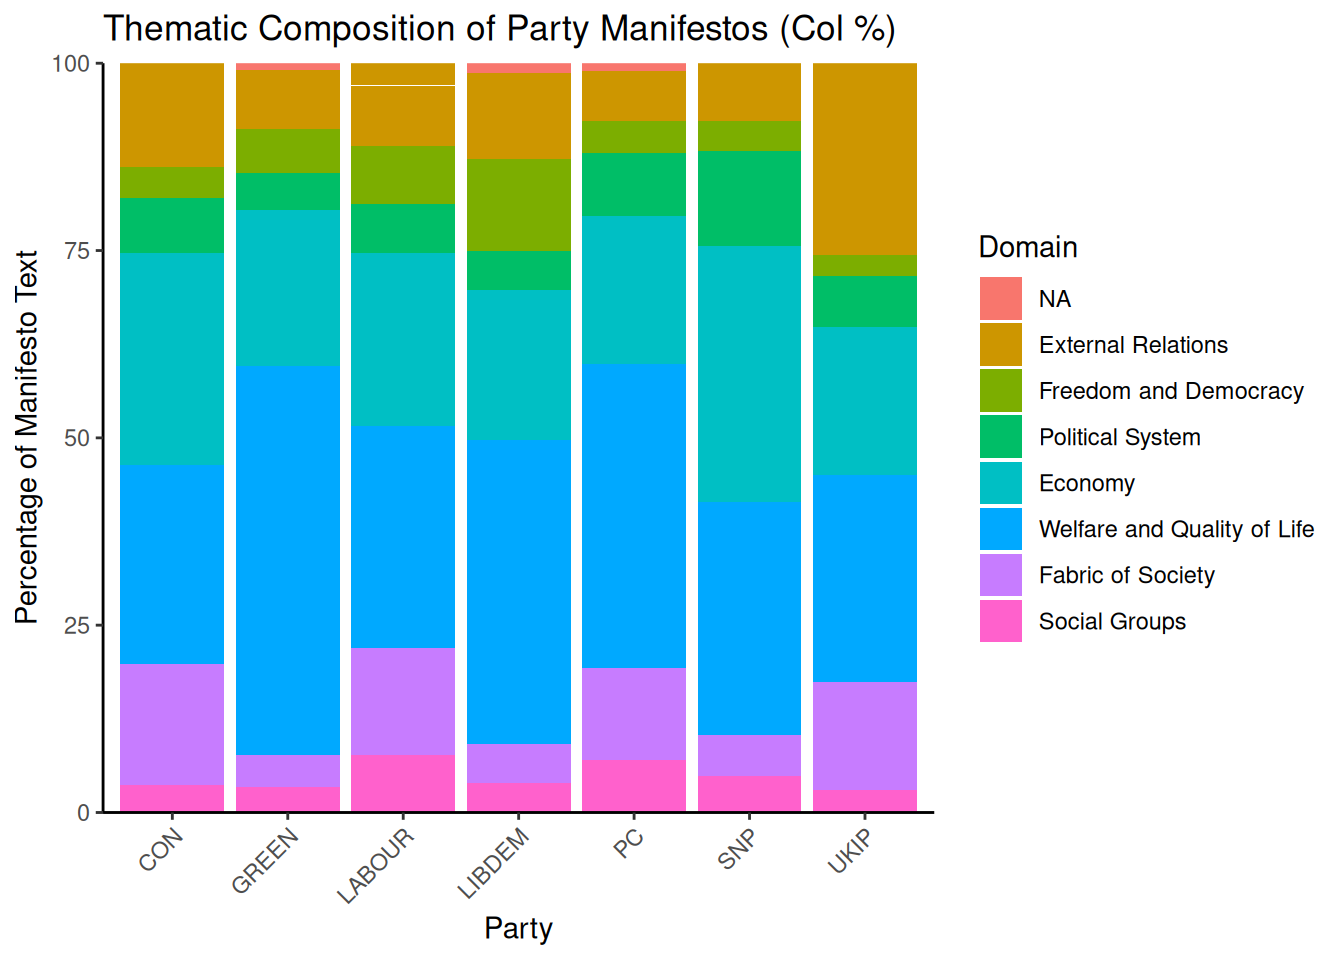
\includegraphics[keepaspectratio]{Introduction-to-Quantitative-Text-Analysis_files/figure-latex/ggplot-nb-domains-1.pdf}}

The plot shows that ``Welfare and Quality of Life'' and ``Economy'' are dominant themes across most parties. We can also see party-specific focuses, such as UKIP's emphasis on ``External Relations''.

Now, let us turn to the Naive Bayes. First, she place our data into a corpus object:

\begin{Shaded}
\begin{Highlighting}[]
\NormalTok{manifesto\_corpus }\OtherTok{\textless{}{-}} \FunctionTok{corpus}\NormalTok{(manifesto\_data, }\AttributeTok{text\_field =} \StringTok{"texts"}\NormalTok{)}
\FunctionTok{summary}\NormalTok{(manifesto\_corpus, }\DecValTok{10}\NormalTok{)}
\end{Highlighting}
\end{Shaded}

\begin{verbatim}
## Corpus consisting of 9763 documents, showing 10 documents:
## 
##             Text Types Tokens Sentences cmp_code  party
##   51320_201505.7    13     14         1      414 LABOUR
##   51320_201505.8    29     35         1      414 LABOUR
##  51320_201505.10     9      9         1      414 LABOUR
##  51320_201505.11     7      7         1      414 LABOUR
##  51320_201505.12    17     17         1      414 LABOUR
##  51320_201505.13    21     22         1      414 LABOUR
##  51320_201505.14    10     10         1      414 LABOUR
##  51320_201505.15    18     20         1      414 LABOUR
##  51320_201505.16    26     30         1      414 LABOUR
##  51320_201505.17    20     22         1      414 LABOUR
\end{verbatim}

To train and evaluate our model, we must split the data into training and test sets. We'll use 80\% for training and 20\% for testing. \texttt{set.seed} ensures that the random sampling is reproducible.

\begin{Shaded}
\begin{Highlighting}[]
\FunctionTok{set.seed}\NormalTok{(}\DecValTok{42}\NormalTok{)}

\CommentTok{\# Generate a random sample of document indices for the training set}
\NormalTok{id\_train }\OtherTok{\textless{}{-}} \FunctionTok{sample}\NormalTok{(}\DecValTok{1}\SpecialCharTok{:}\FunctionTok{ndoc}\NormalTok{(manifesto\_corpus), }\AttributeTok{size =} \FunctionTok{ndoc}\NormalTok{(manifesto\_corpus) }\SpecialCharTok{*} \FloatTok{0.8}\NormalTok{,}
    \AttributeTok{replace =} \ConstantTok{FALSE}\NormalTok{)}

\CommentTok{\# Create training and test sets by subsetting the corpus}
\NormalTok{train\_corpus }\OtherTok{\textless{}{-}} \FunctionTok{corpus\_subset}\NormalTok{(manifesto\_corpus, }\DecValTok{1}\SpecialCharTok{:}\FunctionTok{ndoc}\NormalTok{(manifesto\_corpus) }\SpecialCharTok{\%in\%}\NormalTok{ id\_train)}
\NormalTok{test\_corpus }\OtherTok{\textless{}{-}} \FunctionTok{corpus\_subset}\NormalTok{(manifesto\_corpus, }\SpecialCharTok{!}\DecValTok{1}\SpecialCharTok{:}\FunctionTok{ndoc}\NormalTok{(manifesto\_corpus) }\SpecialCharTok{\%in\%}\NormalTok{ id\_train)}
\end{Highlighting}
\end{Shaded}

Next, we create Document-Feature Matrices (DFMs) from our corpus subsets. A DFM is a table where rows represent documents, columns represent words (features), and cells contain word counts. We perform basic text cleaning during this step: removing punctuation, numbers, and symbols. We also trim the DFM to remove very infrequent terms, which helps reduce noise and improve model performance.

\begin{Shaded}
\begin{Highlighting}[]
\CommentTok{\# Create DFM for the training set}
\NormalTok{train\_dfm }\OtherTok{\textless{}{-}}\NormalTok{ train\_corpus }\SpecialCharTok{\%\textgreater{}\%}
    \FunctionTok{tokens}\NormalTok{(}\AttributeTok{remove\_punct =} \ConstantTok{TRUE}\NormalTok{, }\AttributeTok{remove\_numbers =} \ConstantTok{TRUE}\NormalTok{, }\AttributeTok{remove\_symbols =} \ConstantTok{TRUE}\NormalTok{) }\SpecialCharTok{\%\textgreater{}\%}
    \FunctionTok{dfm}\NormalTok{() }\SpecialCharTok{\%\textgreater{}\%}
    \FunctionTok{dfm\_trim}\NormalTok{(}\AttributeTok{min\_termfreq =} \DecValTok{5}\NormalTok{)}

\CommentTok{\# Create DFM for the test set We don\textquotesingle{}t trim the test set yet, as we will match}
\CommentTok{\# its features to the training set}
\NormalTok{test\_dfm }\OtherTok{\textless{}{-}}\NormalTok{ test\_corpus }\SpecialCharTok{\%\textgreater{}\%}
    \FunctionTok{tokens}\NormalTok{(}\AttributeTok{remove\_punct =} \ConstantTok{TRUE}\NormalTok{, }\AttributeTok{remove\_numbers =} \ConstantTok{TRUE}\NormalTok{, }\AttributeTok{remove\_symbols =} \ConstantTok{TRUE}\NormalTok{) }\SpecialCharTok{\%\textgreater{}\%}
    \FunctionTok{dfm}\NormalTok{()}
\end{Highlighting}
\end{Shaded}

We train the Naive Bayes model using the training DFM and the \texttt{cmp\_code} variable as the target label.

\begin{Shaded}
\begin{Highlighting}[]
\NormalTok{manifesto\_nb }\OtherTok{\textless{}{-}} \FunctionTok{textmodel\_nb}\NormalTok{(train\_dfm, }\AttributeTok{y =} \FunctionTok{docvars}\NormalTok{(train\_corpus, }\StringTok{"cmp\_code"}\NormalTok{))}
\FunctionTok{summary}\NormalTok{(manifesto\_nb)}
\end{Highlighting}
\end{Shaded}

The model summary provides estimated feature scores (the probability of a word given a class). We aim to evaluate the model's performance on unseen data from the test set. Keep in mind that the Naive Bayes model can only make predictions based on features it has seen during training. Therefore, we must align the feature set of the test DFM with the training DFM. The \texttt{dfm\_match()} function ensures that the test DFM has the same features as the training DFM.

\begin{Shaded}
\begin{Highlighting}[]
\NormalTok{matched\_test\_dfm }\OtherTok{\textless{}{-}} \FunctionTok{dfm\_match}\NormalTok{(test\_dfm, }\AttributeTok{features =} \FunctionTok{featnames}\NormalTok{(train\_dfm))}
\end{Highlighting}
\end{Shaded}

The number of features in the matched test DFM is now identical to the training DFM. We can now predict the classes for the test set.

\begin{Shaded}
\begin{Highlighting}[]
\CommentTok{\# Predict the classes for the matched test set}
\NormalTok{predicted\_class }\OtherTok{\textless{}{-}} \FunctionTok{predict}\NormalTok{(manifesto\_nb, }\AttributeTok{newdata =}\NormalTok{ matched\_test\_dfm)}

\CommentTok{\# Get the actual classes from the test corpus\textquotesingle{}s document variables}
\NormalTok{actual\_class }\OtherTok{\textless{}{-}} \FunctionTok{docvars}\NormalTok{(test\_corpus, }\StringTok{"cmp\_code"}\NormalTok{)}

\CommentTok{\# Create a confusion matrix (table of actual vs. predicted classes)}
\NormalTok{table\_class }\OtherTok{\textless{}{-}} \FunctionTok{table}\NormalTok{(}\AttributeTok{Actual =}\NormalTok{ actual\_class, }\AttributeTok{Predicted =}\NormalTok{ predicted\_class)}

\CommentTok{\# Display a subset of the confusion matrix due to its large size}
\NormalTok{table\_class[}\DecValTok{1}\SpecialCharTok{:}\DecValTok{10}\NormalTok{, }\DecValTok{1}\SpecialCharTok{:}\DecValTok{10}\NormalTok{]}
\end{Highlighting}
\end{Shaded}

\begin{verbatim}
##       Predicted
## Actual  0 101 103 104 105 106 107 108 109 110
##    0    0   0   0   0   0   0   1   0   0   1
##    101  0   0   0   1   0   0   1   0   0   0
##    104  1   0   0  16   0   0   0   0   0   4
##    105  0   0   0   2   5   1   1   0   0   1
##    106  0   0   0   0   0   1   2   1   0   0
##    107  0   0   0   3   0   0  24   0   0   3
##    108  0   0   0   1   0   0   0   6   0   8
##    109  0   0   0   0   0   0   0   0   0   2
##    110  0   0   0   0   0   0   0   2   0  42
##    201  0   1   0   0   0   0   1   0   0   0
\end{verbatim}

A confusion matrix table can be large and difficult to interpret. A heatmap offers a more intuitive visualization, highlighting where the model is accurate (strong diagonal) and where it makes errors (dark cells off the diagonal).

\begin{Shaded}
\begin{Highlighting}[]
\CommentTok{\# Convert the table to a data frame for plotting}
\NormalTok{table\_class\_df }\OtherTok{\textless{}{-}} \FunctionTok{as.data.frame}\NormalTok{(table\_class)}
\FunctionTok{names}\NormalTok{(table\_class\_df) }\OtherTok{\textless{}{-}} \FunctionTok{c}\NormalTok{(}\StringTok{"Actual"}\NormalTok{, }\StringTok{"Predicted"}\NormalTok{, }\StringTok{"Frequency"}\NormalTok{)}

\CommentTok{\# Plot the confusion matrix as a heatmap}
\FunctionTok{ggplot}\NormalTok{(}\AttributeTok{data =}\NormalTok{ table\_class\_df, }\FunctionTok{aes}\NormalTok{(}\AttributeTok{x =}\NormalTok{ Predicted, }\AttributeTok{y =}\NormalTok{ Actual)) }\SpecialCharTok{+} \FunctionTok{geom\_tile}\NormalTok{(}\FunctionTok{aes}\NormalTok{(}\AttributeTok{fill =}\NormalTok{ Frequency)) }\SpecialCharTok{+}
    \FunctionTok{scale\_fill\_gradient}\NormalTok{(}\AttributeTok{low =} \StringTok{"white"}\NormalTok{, }\AttributeTok{high =} \StringTok{"\#002366"}\NormalTok{, }\AttributeTok{name =} \StringTok{"Frequency"}\NormalTok{) }\SpecialCharTok{+} \FunctionTok{labs}\NormalTok{(}\AttributeTok{x =} \StringTok{"Predicted Class"}\NormalTok{,}
    \AttributeTok{y =} \StringTok{"Actual Class"}\NormalTok{, }\AttributeTok{title =} \StringTok{"Confusion Matrix: Actual vs. Predicted Manifesto Codes"}\NormalTok{) }\SpecialCharTok{+}
    \FunctionTok{theme\_classic}\NormalTok{() }\SpecialCharTok{+} \FunctionTok{theme}\NormalTok{(}\AttributeTok{axis.text.x =} \FunctionTok{element\_text}\NormalTok{(}\AttributeTok{angle =} \DecValTok{90}\NormalTok{, }\AttributeTok{vjust =} \FloatTok{0.5}\NormalTok{, }\AttributeTok{size =} \DecValTok{8}\NormalTok{),}
    \AttributeTok{axis.text.y =} \FunctionTok{element\_text}\NormalTok{(}\AttributeTok{size =} \DecValTok{8}\NormalTok{))}
\end{Highlighting}
\end{Shaded}

\pandocbounded{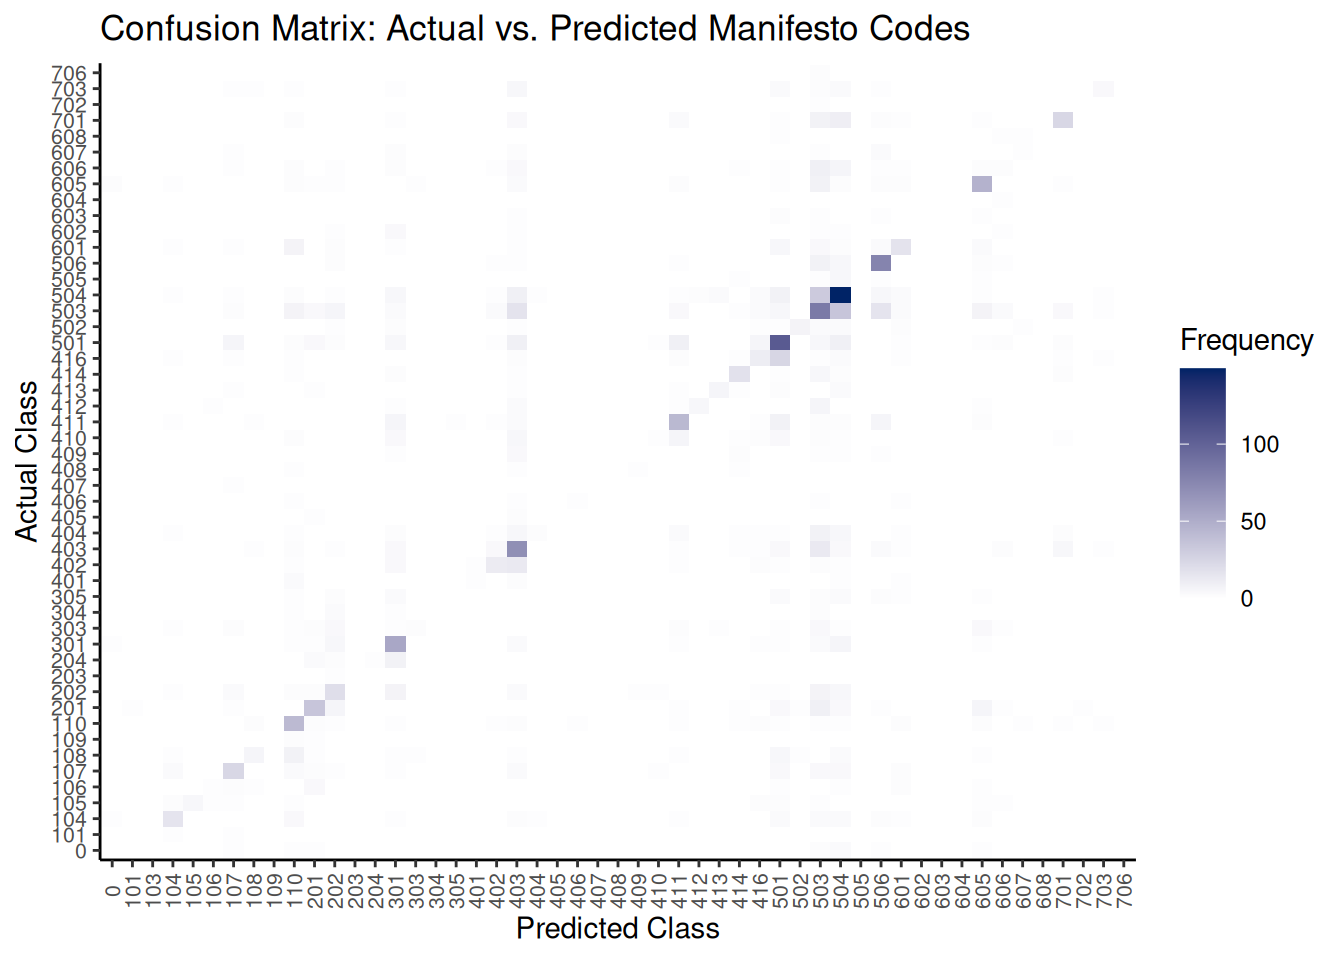
\includegraphics[keepaspectratio]{Introduction-to-Quantitative-Text-Analysis_files/figure-latex/ggplot-nb-heatmap-1.pdf}}

To further understand how well NB has done, we can calculate aggregate performance metrics like accuracy, precision, recall, and F1-score. The \texttt{caret} package's \texttt{confusionMatrix} function is ideal.

\begin{Shaded}
\begin{Highlighting}[]
\CommentTok{\# Ensure levels are consistent for the confusion matrix function}
\NormalTok{all\_levels }\OtherTok{\textless{}{-}} \FunctionTok{unique}\NormalTok{(}\FunctionTok{c}\NormalTok{(}\FunctionTok{as.character}\NormalTok{(actual\_class), }\FunctionTok{as.character}\NormalTok{(predicted\_class)))}
\NormalTok{actual\_class\_factor }\OtherTok{\textless{}{-}} \FunctionTok{factor}\NormalTok{(actual\_class, }\AttributeTok{levels =}\NormalTok{ all\_levels)}
\NormalTok{predicted\_class\_factor }\OtherTok{\textless{}{-}} \FunctionTok{factor}\NormalTok{(predicted\_class, }\AttributeTok{levels =}\NormalTok{ all\_levels)}

\CommentTok{\# Calculate various classification metrics using caret::confusionMatrix}
\NormalTok{classification\_metrics }\OtherTok{\textless{}{-}} \FunctionTok{confusionMatrix}\NormalTok{(predicted\_class\_factor, actual\_class\_factor)}

\CommentTok{\# Display macro{-}averaged F1{-}score (calculated manually from per{-}class stats)}
\NormalTok{macro\_f1 }\OtherTok{\textless{}{-}} \FunctionTok{mean}\NormalTok{(classification\_metrics}\SpecialCharTok{$}\NormalTok{byClass[, }\StringTok{"F1"}\NormalTok{], }\AttributeTok{na.rm =} \ConstantTok{TRUE}\NormalTok{)}
\FunctionTok{cat}\NormalTok{(}\StringTok{"Macro{-}Averaged F1{-}Score:"}\NormalTok{, macro\_f1, }\StringTok{"}\SpecialCharTok{\textbackslash{}n}\StringTok{"}\NormalTok{)}
\end{Highlighting}
\end{Shaded}

\begin{verbatim}
## Macro-Averaged F1-Score: 0.3686071
\end{verbatim}

In addition to this, comparing the frequency distribution of predicted classes against the actual classes can reveal if the model is biased towards or against specific categories.

\begin{Shaded}
\begin{Highlighting}[]
\CommentTok{\# Create data frames for actual and predicted class counts and combine them}
\NormalTok{actual\_counts\_df }\OtherTok{\textless{}{-}} \FunctionTok{as.data.frame}\NormalTok{(}\FunctionTok{table}\NormalTok{(actual\_class), }\AttributeTok{stringsAsFactors =} \ConstantTok{FALSE}\NormalTok{) }\SpecialCharTok{\%\textgreater{}\%}
    \FunctionTok{rename}\NormalTok{(}\AttributeTok{Code =}\NormalTok{ actual\_class, }\AttributeTok{Frequency =}\NormalTok{ Freq) }\SpecialCharTok{\%\textgreater{}\%}
    \FunctionTok{mutate}\NormalTok{(}\AttributeTok{Type =} \StringTok{"Actual"}\NormalTok{)}

\NormalTok{predicted\_counts\_df }\OtherTok{\textless{}{-}} \FunctionTok{as.data.frame}\NormalTok{(}\FunctionTok{table}\NormalTok{(predicted\_class), }\AttributeTok{stringsAsFactors =} \ConstantTok{FALSE}\NormalTok{) }\SpecialCharTok{\%\textgreater{}\%}
    \FunctionTok{rename}\NormalTok{(}\AttributeTok{Code =}\NormalTok{ predicted\_class, }\AttributeTok{Frequency =}\NormalTok{ Freq) }\SpecialCharTok{\%\textgreater{}\%}
    \FunctionTok{mutate}\NormalTok{(}\AttributeTok{Type =} \StringTok{"Predicted"}\NormalTok{)}

\NormalTok{class\_distribution\_df }\OtherTok{\textless{}{-}} \FunctionTok{bind\_rows}\NormalTok{(actual\_counts\_df, predicted\_counts\_df)}

\CommentTok{\# Plot the distribution}
\FunctionTok{ggplot}\NormalTok{(class\_distribution\_df, }\FunctionTok{aes}\NormalTok{(}\AttributeTok{x =}\NormalTok{ Code, }\AttributeTok{y =}\NormalTok{ Frequency, }\AttributeTok{fill =}\NormalTok{ Type)) }\SpecialCharTok{+} \FunctionTok{geom\_bar}\NormalTok{(}\AttributeTok{stat =} \StringTok{"identity"}\NormalTok{,}
    \AttributeTok{position =} \StringTok{"dodge"}\NormalTok{) }\SpecialCharTok{+} \FunctionTok{theme\_classic}\NormalTok{() }\SpecialCharTok{+} \FunctionTok{labs}\NormalTok{(}\AttributeTok{x =} \StringTok{"Manifesto Code"}\NormalTok{, }\AttributeTok{y =} \StringTok{"Number of Sentences"}\NormalTok{,}
    \AttributeTok{title =} \StringTok{"Distribution of Actual vs. Predicted Manifesto Codes"}\NormalTok{) }\SpecialCharTok{+} \FunctionTok{scale\_fill\_manual}\NormalTok{(}\AttributeTok{values =} \FunctionTok{c}\NormalTok{(}\AttributeTok{Actual =} \StringTok{"\#0087DC"}\NormalTok{,}
    \AttributeTok{Predicted =} \StringTok{"\#DC241F"}\NormalTok{)) }\SpecialCharTok{+} \FunctionTok{theme}\NormalTok{(}\AttributeTok{axis.text.x =} \FunctionTok{element\_text}\NormalTok{(}\AttributeTok{angle =} \DecValTok{90}\NormalTok{, }\AttributeTok{vjust =} \FloatTok{0.5}\NormalTok{,}
    \AttributeTok{size =} \DecValTok{8}\NormalTok{))}
\end{Highlighting}
\end{Shaded}

\pandocbounded{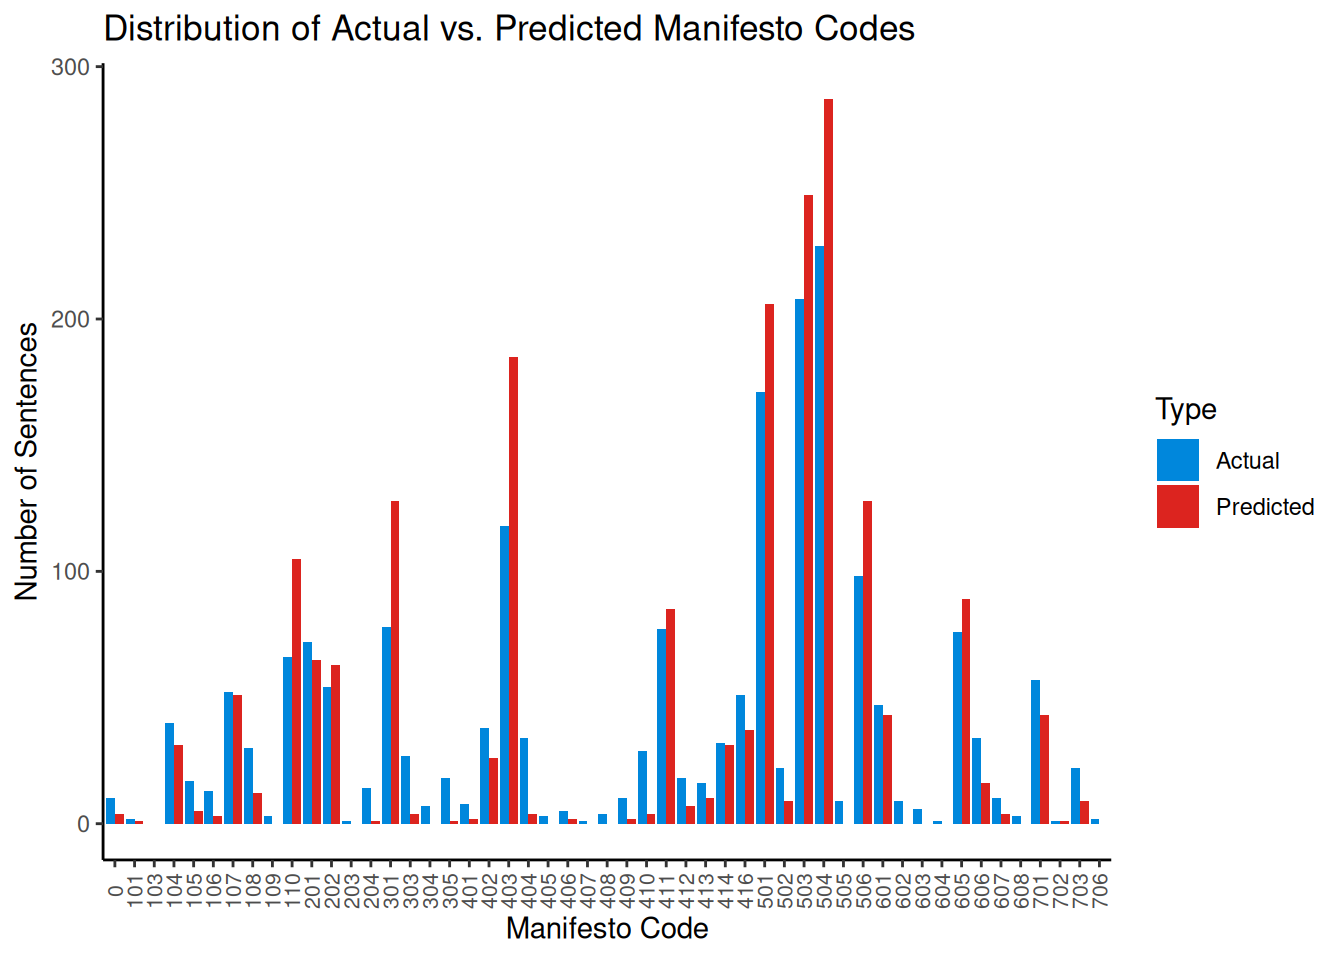
\includegraphics[keepaspectratio]{Introduction-to-Quantitative-Text-Analysis_files/figure-latex/ggplot-class-distribution-1.pdf}}

This plot helps visualize if the model over-predicts (red bar is taller) or under-predicts (blue bar is taller) specific codes compared to their true frequency in the test set.

Finally, we can use Krippendorff's \(\alpha\) again to measure the agreement between the model's predictions and the human-assigned codes, accounting for chance agreement.

\begin{Shaded}
\begin{Highlighting}[]
\NormalTok{reliability\_data }\OtherTok{\textless{}{-}} \FunctionTok{as.matrix}\NormalTok{(}\FunctionTok{rbind}\NormalTok{(}\FunctionTok{as.character}\NormalTok{(actual\_class), }\FunctionTok{as.character}\NormalTok{(predicted\_class)))}

\CommentTok{\# Calculate for nominal data}
\NormalTok{kripp\_alpha }\OtherTok{\textless{}{-}} \FunctionTok{KrippAlpha}\NormalTok{(reliability\_data, }\AttributeTok{method =} \StringTok{"nominal"}\NormalTok{)}
\NormalTok{kripp\_alpha}\SpecialCharTok{$}\NormalTok{value}
\end{Highlighting}
\end{Shaded}

\begin{verbatim}
## [1] 0.420661
\end{verbatim}

Interpreting the \(\alpha\) value requires context. Research by Mikhaylov et al. (\citeproc{ref-Mikhaylov2012a}{2012}) estimates the agreement \emph{among trained human coders} for the Manifesto Project to be between 0.350 and 0.400. Seen this way, our \(\alpha = 0.43\) from our simple automated model is therefore quite good!

\section{Exercises}\label{exercises-3}

\begin{enumerate}
\def\labelenumi{\arabic{enumi}.}
\item
  Modify the \texttt{caret} SVM example to use TF-IDF weighting for the DFM rather than raw term frequency. Does this affect the performance of the SVM model when evaluated using cross-validation?
\item
  Using the movie review sentiment data, train a logistic regression model with the \texttt{glmnet} method using the \texttt{caret::train()} function (ensure you have the \texttt{glmnet} package installed). Use cross-validation for training. Compare the performance of this model with that of the SVM model using a confusion matrix, an ROC-AUC plot, and a calibration plot.
\item
  Investigate the impact of various pre-processing steps (e.g.~removing numbers, stemming versus non-stemming and using bigrams) on the performance of the Naive Bayes model with the Manifesto Project data. Evaluate performance using cross-validation and compare confusion matrices.
\item
  Investigate how to deal with imbalanced classes in text classification. For a dataset with imbalanced classes, research a relevant technique (e.g.~the ROSE package or the sampling options in the \texttt{trainControl} function of the \texttt{caret} package) and apply it during cross-validated training. Does this improve the performance of the minority class compared to training without addressing the imbalance?
\item
  For either the SVM or Naive Bayes model, research how to tune hyperparameters using the \texttt{tuneGrid} argument in \texttt{caret::train()}. Implement a simple hyperparameter tuning process using cross-validation, then report on the performance of the best-tuned model.
\end{enumerate}

\chapter{Unsupervised Methods}\label{unsupervised-methods}

Unlike supervised methods, which require labelled data to train a model for classifying or predicting values for new text, unsupervised learning methods in text analysis aim to discover inherent patterns and structures within text data without relying on pre-assigned labels.
These methods are useful for exploring large unannotated corpora to identify recurring themes (topics), group similar documents (clustering) and reduce the dimensionality of the data.

Supervised models excel at well-defined classification tasks where labelled data is available, but unsupervised methods allow us to uncover latent structures that we may not have anticipated or would be prohibitively expensive to label.
This chapter focuses on probabilistic topic modelling, a popular suite of unsupervised methods for identifying abstract `topics' within a body of text.
Each document is treated as a mixture of these topics, with a word distribution characterising each.
We will cover Latent Dirichlet Allocation (LDA), seeded LDA, which incorporates prior knowledge, the Structural Topic Model (STM), which allows the inclusion of document metadata to model topic prevalence and content, and Latent Semantic Analysis (LSA) as a dimensionality reduction technique.

The original document provided a solid introduction to these methods.
I have expanded upon the explanations of each technique, particularly focusing on the rationale behind key steps and the interpretation of results.
I have also significantly extended the sections on model validation for LDA, STM, and LSA, as understanding how to evaluate these models is crucial for their practical application.

\section{Latent Dirichlet Allocation (LDA)}\label{latent-dirichlet-allocation-lda}

Latent Dirichlet Allocation (LDA) is a generative probabilistic model for collections of discrete data, such as text corpora.
The core idea is that each document contains various topics, and a word distribution characterises each topic.
The model assumes that the process of writing a document includes:

\begin{enumerate}
\def\labelenumi{\arabic{enumi}.}
\tightlist
\item
  Choosing the length of the document.
\item
  Choosing a mixture of topics for the document.
\item
  For each word in the document:

  \begin{itemize}
  \tightlist
  \item
    Choosing a topic from the mixture of topics in the document.
  \item
    Choosing a word from the word distribution of the selected topic.
  \end{itemize}
\end{enumerate}

LDA aims to infer these latent topic mixtures for each document and word distributions for each topic, given the observed word frequencies in the corpus.

We will primarily use the \texttt{topicmodels} package to run LDA in R.
This package works with a specific document-term matrix format, so we first need to convert our \texttt{quanteda} dfm into this format using the \texttt{convert()} function.
We will use the inaugural speeches corpus (\texttt{data\_inaugural\_dfm}) from previous chapters as our example data.

We begin by loading the necessary libraries.
\texttt{topicmodels} is the core package for LDA.
\texttt{quanteda} is needed for corpus and DFM manipulation.
\texttt{dplyr}, \texttt{tidytext}, and \texttt{ggplot2} are essential for subsequent data manipulation and visualisation of the model outputs in a tidy format.

\begin{Shaded}
\begin{Highlighting}[]
\CommentTok{\# Install topicmodels if you haven\textquotesingle{}t already: install.packages(\textquotesingle{}topicmodels\textquotesingle{})}
\FunctionTok{library}\NormalTok{(topicmodels)}
\FunctionTok{library}\NormalTok{(quanteda)  }\CommentTok{\# Ensure quanteda is loaded}
\FunctionTok{library}\NormalTok{(dplyr)  }\CommentTok{\# For data manipulation later}
\FunctionTok{library}\NormalTok{(tidytext)  }\CommentTok{\# For tidying model output later}
\FunctionTok{library}\NormalTok{(ggplot2)  }\CommentTok{\# For visualization later}


\FunctionTok{data}\NormalTok{(data\_corpus\_inaugural)}
\NormalTok{data\_inaugural\_tokens }\OtherTok{\textless{}{-}} \FunctionTok{tokens}\NormalTok{(data\_corpus\_inaugural, }\AttributeTok{remove\_punct =} \ConstantTok{TRUE}\NormalTok{, }\AttributeTok{remove\_symbols =} \ConstantTok{TRUE}\NormalTok{,}
    \AttributeTok{remove\_numbers =} \ConstantTok{TRUE}\NormalTok{, }\AttributeTok{remove\_url =} \ConstantTok{TRUE}\NormalTok{, }\AttributeTok{remove\_separators =} \ConstantTok{TRUE}\NormalTok{, }\AttributeTok{split\_hyphens =} \ConstantTok{FALSE}\NormalTok{)}
\NormalTok{data\_inaugural\_tokens }\OtherTok{\textless{}{-}} \FunctionTok{tokens\_tolower}\NormalTok{(data\_inaugural\_tokens)}
\NormalTok{data\_inaugural\_tokens }\OtherTok{\textless{}{-}} \FunctionTok{tokens\_select}\NormalTok{(data\_inaugural\_tokens, }\FunctionTok{stopwords}\NormalTok{(}\StringTok{"english"}\NormalTok{),}
    \AttributeTok{selection =} \StringTok{"remove"}\NormalTok{)}
\NormalTok{data\_inaugural\_dfm }\OtherTok{\textless{}{-}} \FunctionTok{dfm}\NormalTok{(data\_inaugural\_tokens)}
\NormalTok{data\_inaugural\_dfm }\OtherTok{\textless{}{-}} \FunctionTok{dfm\_compress}\NormalTok{(data\_inaugural\_dfm, }\AttributeTok{margin =} \StringTok{"features"}\NormalTok{)}

\NormalTok{inaugural\_dtm }\OtherTok{\textless{}{-}} \FunctionTok{convert}\NormalTok{(data\_inaugural\_dfm, }\AttributeTok{to =} \StringTok{"topicmodels"}\NormalTok{)}
\end{Highlighting}
\end{Shaded}

Once the libraries have been loaded and the data has been prepared in the required format, we will specify the parameters for the LDA model using Gibbs sampling.
These parameters control the inference process, including the number of iterations, burn-in period, thinning interval, random seeds for reproducibility, and independent chains to run.

When using Gibbs sampling, specific parameters need to be set: \emph{burnin} (the number of initial iterations to discard), \emph{iter} (the total number of iterations after the burn-in period), \emph{thin} (the thinning interval), \emph{seed} (the random seed or seeds for multiple runs), \emph{nstart} (the number of independent chains) and \emph{best} (whether to keep the model with the highest log-likelihood if nstart \textgreater{} 1).
Additionally, we must set the desired number of topics to extract.
This is a common challenge in topic modelling, as no definitive method exists.
It often involves a combination of statistical measures, such as likelihood or coherence scores, and qualitative evaluation of the topics to determine their meaning and interpretability.

Using Gibbs sampling, we can fit an LDA model with a chosen number of topics.
For example, k could be set to 10.
The explanation of the parameters and the choice of k has been expanded slightly for clarity.

\begin{Shaded}
\begin{Highlighting}[]
\CommentTok{\# Set parameters for Gibbs sampling}
\NormalTok{burnin }\OtherTok{\textless{}{-}} \DecValTok{2000}  \CommentTok{\# Number of initial iterations to discard.}
\NormalTok{iter }\OtherTok{\textless{}{-}} \DecValTok{1000}  \CommentTok{\# Number of iterations to keep after burnin.}
\NormalTok{thin }\OtherTok{\textless{}{-}} \DecValTok{200}  \CommentTok{\# Keep every 200th iteration.}
\NormalTok{seed }\OtherTok{\textless{}{-}} \FunctionTok{list}\NormalTok{(}\DecValTok{42}\NormalTok{, }\DecValTok{5}\NormalTok{, }\DecValTok{24}\NormalTok{, }\DecValTok{158}\NormalTok{, }\DecValTok{2500}\NormalTok{)  }\CommentTok{\# Seeds for multiple runs. }
\NormalTok{nstart }\OtherTok{\textless{}{-}} \DecValTok{5}  \CommentTok{\# Number of independent chains to run.}
\NormalTok{best }\OtherTok{\textless{}{-}} \ConstantTok{TRUE}  \CommentTok{\# Keep the best model from the multiple runs. }
\NormalTok{k\_lda }\OtherTok{\textless{}{-}} \DecValTok{10}  \CommentTok{\# Number of topics to find. }
\end{Highlighting}
\end{Shaded}

With the parameters defined, we fit the LDA model to the document-term matrix.
The \texttt{LDA()} function from the \texttt{topicmodels} package performs this fitting process using the specified method and control parameters.

\begin{Shaded}
\begin{Highlighting}[]
\CommentTok{\# Fit the LDA model using Gibbs sampling}
\NormalTok{inaugural\_lda10 }\OtherTok{\textless{}{-}} \FunctionTok{LDA}\NormalTok{(inaugural\_dtm, }\AttributeTok{k =}\NormalTok{ k\_lda, }\AttributeTok{method =} \StringTok{"Gibbs"}\NormalTok{, }\AttributeTok{control =} \FunctionTok{list}\NormalTok{(}\AttributeTok{burnin =}\NormalTok{ burnin,}
    \AttributeTok{iter =}\NormalTok{ iter, }\AttributeTok{thin =}\NormalTok{ thin, }\AttributeTok{seed =}\NormalTok{ seed, }\AttributeTok{nstart =}\NormalTok{ nstart, }\AttributeTok{best =}\NormalTok{ best))}

\CommentTok{\# Display the top words for each topic}
\FunctionTok{print}\NormalTok{(}\StringTok{"Top terms per topic:"}\NormalTok{)}
\end{Highlighting}
\end{Shaded}

\begin{verbatim}
## [1] "Top terms per topic:"
\end{verbatim}

\begin{Shaded}
\begin{Highlighting}[]
\FunctionTok{terms}\NormalTok{(inaugural\_lda10, }\DecValTok{10}\NormalTok{)  }\CommentTok{\# Show top 10 terms for each of the 10 topics. These terms are the words with the highest probability within each topic.}
\end{Highlighting}
\end{Shaded}

\begin{verbatim}
##       Topic 1    Topic 2    Topic 3    Topic 4   Topic 5        Topic 6       
##  [1,] "world"    "will"     "life"     "will"    "shall"        "union"       
##  [2,] "peace"    "must"     "spirit"   "us"      "states"       "constitution"
##  [3,] "nations"  "make"     "things"   "america" "now"          "can"         
##  [4,] "free"     "business" "nation"   "can"     "will"         "one"         
##  [5,] "must"     "american" "men"      "people"  "constitution" "states"      
##  [6,] "freedom"  "made"     "task"     "nation"  "congress"     "state"       
##  [7,] "can"      "trade"    "purpose"  "one"     "upon"         "free"        
##  [8,] "new"      "secure"   "problems" "new"     "great"        "among"       
##  [9,] "men"      "law"      "without"  "must"    "years"        "within"      
## [10,] "progress" "can"      "action"   "world"   "laws"         "blessings"   
##       Topic 7      Topic 8    Topic 9     Topic 10    
##  [1,] "freedom"    "war"      "great"     "government"
##  [2,] "let"        "just"     "may"       "people"    
##  [3,] "time"       "nations"  "power"     "will"      
##  [4,] "citizens"   "united"   "well"      "upon"      
##  [5,] "man"        "every"    "whole"     "country"   
##  [6,] "earth"      "powers"   "states"    "public"    
##  [7,] "generation" "duties"   "might"     "every"     
##  [8,] "human"      "commerce" "executive" "rights"    
##  [9,] "liberty"    "citizens" "time"      "national"  
## [10,] "courage"    "states"   "state"     "interests"
\end{verbatim}

The \texttt{terms()} function allows us to inspect the words with the highest probability of belonging to each topic.
These top words provide initial clues for interpreting the meaning of each discovered topic.
By examining the words associated with each topic, we can begin to understand the themes present in the corpus.

To further explore the topic-word distributions, known as \(\beta\), and prepare them for visualization, we use the \texttt{tidy()} function from the \texttt{tidytext} package.
\texttt{tidytext} facilitates working with text data and model outputs in a ``tidy'' format, which is compatible with \texttt{dplyr} and \texttt{ggplot2} for efficient data manipulation and visualization.

\begin{Shaded}
\begin{Highlighting}[]
\FunctionTok{library}\NormalTok{(tidytext)  }\CommentTok{\# Ensure tidytext is loaded}
\FunctionTok{library}\NormalTok{(dplyr)  }\CommentTok{\# Ensure dplyr is loaded}
\FunctionTok{library}\NormalTok{(ggplot2)  }\CommentTok{\# Ensure ggplot2 is loaded}

\CommentTok{\# Tidy the LDA model output to get the topic{-}word probabilities (beta) The}
\CommentTok{\# \textquotesingle{}beta\textquotesingle{} matrix represents the probability of a word belonging to a topic.}
\NormalTok{inaugural\_lda10\_topics }\OtherTok{\textless{}{-}} \FunctionTok{tidy}\NormalTok{(inaugural\_lda10, }\AttributeTok{matrix =} \StringTok{"beta"}\NormalTok{)}

\CommentTok{\# Display the structure of the tidied beta output}
\FunctionTok{print}\NormalTok{(inaugural\_lda10\_topics)}
\end{Highlighting}
\end{Shaded}

\begin{verbatim}
## # A tibble: 92,090 x 3
##    topic term                  beta
##    <int> <chr>                <dbl>
##  1     1 fellow-citizens 0.0000142 
##  2     2 fellow-citizens 0.000167  
##  3     3 fellow-citizens 0.0000233 
##  4     4 fellow-citizens 0.00000746
##  5     5 fellow-citizens 0.00124   
##  6     6 fellow-citizens 0.0000164 
##  7     7 fellow-citizens 0.0000181 
##  8     8 fellow-citizens 0.0000150 
##  9     9 fellow-citizens 0.00426   
## 10    10 fellow-citizens 0.00000728
## # i 92,080 more rows
\end{verbatim}

The resulting \texttt{inaugural\_lda10\_topics} data frame contains columns for the \texttt{topic}, the \texttt{term} (word), and \texttt{beta} (the probability of that word occurring in that topic).
To visualize the top words for each topic, we filter this data frame to retain only the top N words per topic based on their beta values, typically the top 10, before creating a bar chart.

We select the top terms for each topic based on their beta values, grouping the data by topic and then using \texttt{slice\_max} to select the top 10 terms within each group.
Finally, we arrange the results for better readability.

\begin{Shaded}
\begin{Highlighting}[]
\CommentTok{\# Select the top 10 terms for each topic based on beta values}
\NormalTok{inaugural\_lda10\_topterms }\OtherTok{\textless{}{-}}\NormalTok{ inaugural\_lda10\_topics }\SpecialCharTok{\%\textgreater{}\%}
  \FunctionTok{group\_by}\NormalTok{(topic) }\SpecialCharTok{\%\textgreater{}\%}          \CommentTok{\# Group the data by topic}
  \FunctionTok{slice\_max}\NormalTok{(beta, }\AttributeTok{n =} \DecValTok{10}\NormalTok{) }\SpecialCharTok{\%\textgreater{}\%} 
  \FunctionTok{ungroup}\NormalTok{() }\SpecialCharTok{\%\textgreater{}\%}                
  \FunctionTok{arrange}\NormalTok{(topic, }\SpecialCharTok{{-}}\NormalTok{beta)        }
\end{Highlighting}
\end{Shaded}

Using the filtered data, we create a faceted bar chart to visualize the top terms for each topic and their corresponding beta probabilities.
Reordering the terms within each facet based on their beta values makes the plot easier to interpret.
The explanation of the plot has been slightly expanded.

\begin{Shaded}
\begin{Highlighting}[]
\NormalTok{inaugural\_lda10\_topterms }\SpecialCharTok{\%\textgreater{}\%}
  \FunctionTok{mutate}\NormalTok{(}\AttributeTok{term =} \FunctionTok{reorder\_within}\NormalTok{(term, beta, topic)) }\SpecialCharTok{\%\textgreater{}\%} 
  \FunctionTok{ggplot}\NormalTok{(}\FunctionTok{aes}\NormalTok{(beta, term, }\AttributeTok{fill =} \FunctionTok{factor}\NormalTok{(topic))) }\SpecialCharTok{+}      \CommentTok{\# Plot beta on the x{-}axis, term on the y{-}axis.}
  \FunctionTok{geom\_col}\NormalTok{(}\AttributeTok{show.legend =} \ConstantTok{FALSE}\NormalTok{) }\SpecialCharTok{+}                      \CommentTok{\# Add bars, hide legend}
  \FunctionTok{facet\_wrap}\NormalTok{(}\SpecialCharTok{\textasciitilde{}}\NormalTok{ topic, }\AttributeTok{scales =} \StringTok{"free\_y"}\NormalTok{) }\SpecialCharTok{+}             \CommentTok{\# Create a separate plot (facet) for each topic. }
  \FunctionTok{scale\_y\_reordered}\NormalTok{() }\SpecialCharTok{+}      
  \FunctionTok{labs}\NormalTok{(}\AttributeTok{title =} \StringTok{"Top 10 Words per Topic (LDA Beta)"}\NormalTok{,     }
       \AttributeTok{x =} \StringTok{"Beta (Probability in Topic)"}\NormalTok{,}
       \AttributeTok{y =} \StringTok{"Term"}\NormalTok{) }\SpecialCharTok{+}
  \FunctionTok{theme\_minimal}\NormalTok{() }\CommentTok{\# Use a minimal theme for a clean appearance.}
\end{Highlighting}
\end{Shaded}

\pandocbounded{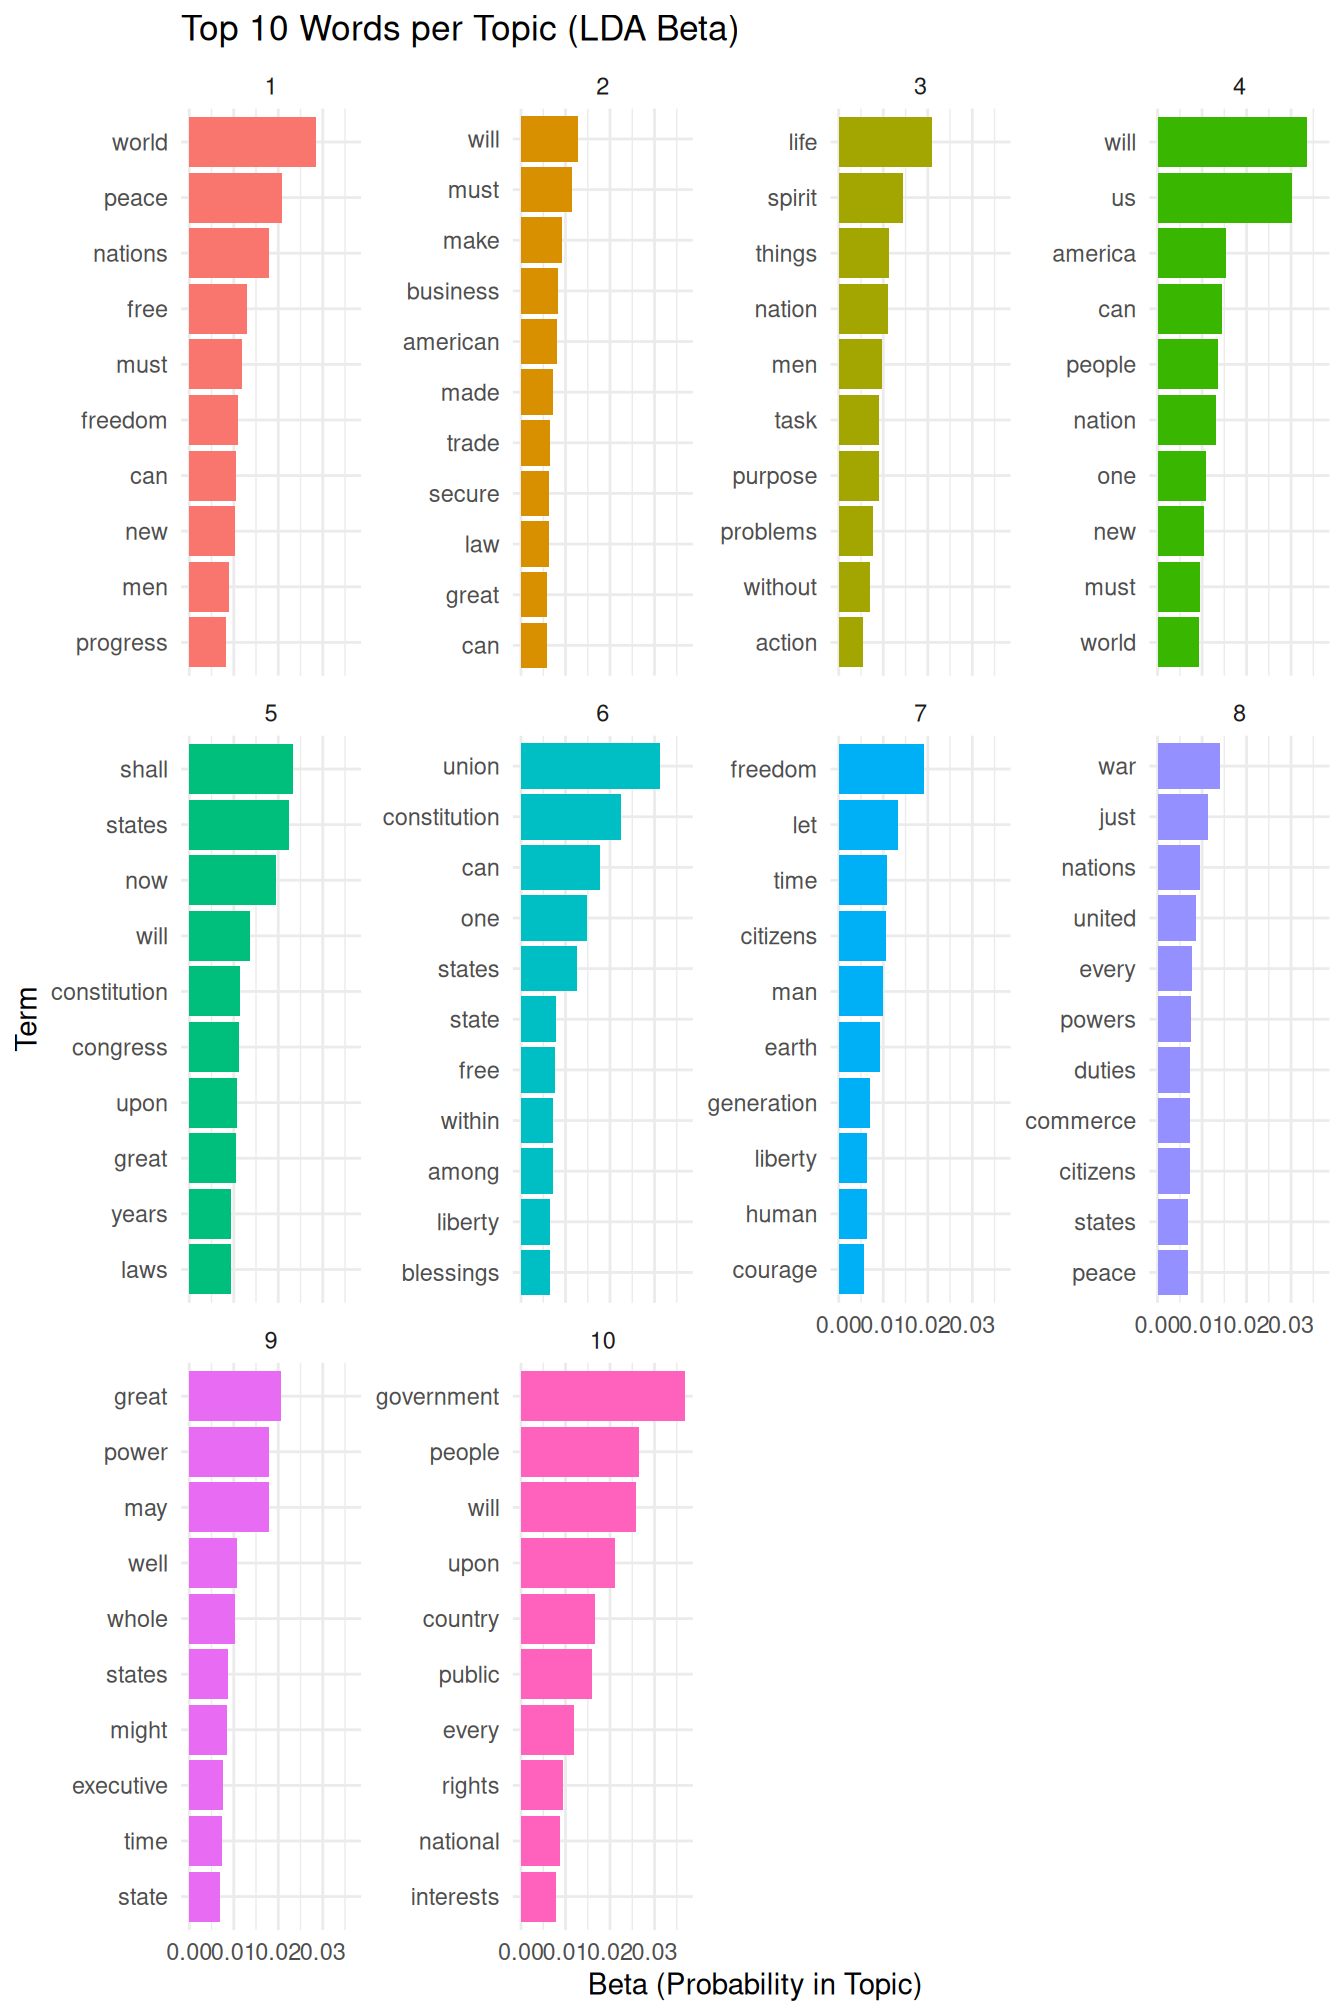
\includegraphics[keepaspectratio]{Introduction-to-Quantitative-Text-Analysis_files/figure-latex/lda-tidy-graph1-1.pdf}}

This plot provides a visual overview of the keywords that define each topic.
By examining these words, we can assign a meaningful label or interpretation to each discovered topic.
This step is crucial for understanding the thematic structure of the corpus.

Another important output of LDA is the document-topic distribution, known as \(\gamma\), which represents the proportion of each topic present in each document. This information allows us to identify which topics are most prominent in specific documents. We again use the \texttt{tidy()} function to extract this data in a convenient format.

\begin{Shaded}
\begin{Highlighting}[]
\CommentTok{\# Tidy the LDA model output to get the document{-}topic probabilities (gamma) The}
\CommentTok{\# \textquotesingle{}gamma\textquotesingle{} matrix represents the proportion of each topic in each document.}
\NormalTok{inaugural\_lda10\_documents }\OtherTok{\textless{}{-}} \FunctionTok{tidy}\NormalTok{(inaugural\_lda10, }\AttributeTok{matrix =} \StringTok{"gamma"}\NormalTok{)}

\CommentTok{\# Display the structure of the tidied gamma output}
\FunctionTok{print}\NormalTok{(inaugural\_lda10\_documents)}
\end{Highlighting}
\end{Shaded}

\begin{verbatim}
## # A tibble: 600 x 3
##    document        topic  gamma
##    <chr>           <int>  <dbl>
##  1 1789-Washington     1 0.0351
##  2 1793-Washington     1 0.0536
##  3 1797-Adams          1 0.0686
##  4 1801-Jefferson      1 0.0594
##  5 1805-Jefferson      1 0.0335
##  6 1809-Madison        1 0.0326
##  7 1813-Madison        1 0.0417
##  8 1817-Monroe         1 0.0159
##  9 1821-Monroe         1 0.0130
## 10 1825-Adams          1 0.0490
## # i 590 more rows
\end{verbatim}

The \texttt{inaugural\_lda10\_documents} data frame contains columns for the \texttt{document}, the \texttt{topic}, and \texttt{gamma} (the proportion of that topic in that document).
We can visualize the topic distribution across documents, for example, by looking at the top topics in a selection of documents or by visualizing the distribution of a specific topic across all documents.
Here, we will visualize the topic distribution for a few selected documents to illustrate how topics are mixed within documents.

We select a subset of documents to visualize their topic distributions.
This allows us to examine the topic proportions in individual documents and see how different topics contribute to the content of each document.

\begin{Shaded}
\begin{Highlighting}[]
\CommentTok{\# Select a few documents to visualise (e.g., the first few)}
\NormalTok{selected\_docs }\OtherTok{\textless{}{-}} \FunctionTok{unique}\NormalTok{(inaugural\_lda10\_documents}\SpecialCharTok{$}\NormalTok{document)[}\DecValTok{1}\SpecialCharTok{:}\DecValTok{5}\NormalTok{] }\CommentTok{\# Select the names of the first 5 unique documents.}

\CommentTok{\# Filter the gamma data for selected documents and arrange}
\NormalTok{inaugural\_lda10\_selected\_docs }\OtherTok{\textless{}{-}}\NormalTok{ inaugural\_lda10\_documents }\SpecialCharTok{\%\textgreater{}\%}
  \FunctionTok{filter}\NormalTok{(document }\SpecialCharTok{\%in\%}\NormalTok{ selected\_docs) }\SpecialCharTok{\%\textgreater{}\%} \CommentTok{\# Keep only the rows where the document name is in our selected\_docs list.}
  \FunctionTok{arrange}\NormalTok{(document, }\SpecialCharTok{{-}}\NormalTok{gamma) }\CommentTok{\# Arrange the data first by document name, then by gamma in descending order to easily see the most prominent topics per document.}

\CommentTok{\# Show the structure of the selected documents\textquotesingle{} gamma data}
\FunctionTok{print}\NormalTok{(inaugural\_lda10\_selected\_docs)}
\end{Highlighting}
\end{Shaded}

\begin{verbatim}
## # A tibble: 50 x 3
##    document        topic  gamma
##    <chr>           <int>  <dbl>
##  1 1789-Washington    10 0.267 
##  2 1789-Washington     8 0.176 
##  3 1789-Washington     9 0.140 
##  4 1789-Washington     6 0.132 
##  5 1789-Washington     5 0.0674
##  6 1789-Washington     2 0.0548
##  7 1789-Washington     4 0.0463
##  8 1789-Washington     3 0.0407
##  9 1789-Washington     7 0.0407
## 10 1789-Washington     1 0.0351
## # i 40 more rows
\end{verbatim}

With the data filtered for the selected documents, we can create a faceted bar plot. This plot shows the proportion of each topic within each of the selected documents, providing a visual representation of the document-topic mixtures.

\begin{Shaded}
\begin{Highlighting}[]
\NormalTok{inaugural\_lda10\_selected\_docs }\SpecialCharTok{\%\textgreater{}\%}
    \FunctionTok{mutate}\NormalTok{(}\AttributeTok{topic =} \FunctionTok{factor}\NormalTok{(topic)) }\SpecialCharTok{\%\textgreater{}\%}
    \FunctionTok{ggplot}\NormalTok{(}\FunctionTok{aes}\NormalTok{(gamma, topic, }\AttributeTok{fill =}\NormalTok{ topic)) }\SpecialCharTok{+} \FunctionTok{geom\_col}\NormalTok{(}\AttributeTok{show.legend =} \ConstantTok{FALSE}\NormalTok{) }\SpecialCharTok{+} \FunctionTok{facet\_wrap}\NormalTok{(}\SpecialCharTok{\textasciitilde{}}\NormalTok{document,}
    \AttributeTok{scales =} \StringTok{"free\_x"}\NormalTok{) }\SpecialCharTok{+} \FunctionTok{labs}\NormalTok{(}\AttributeTok{title =} \StringTok{"Topic Distribution per Document (LDA Gamma)"}\NormalTok{,}
    \AttributeTok{x =} \StringTok{"Gamma (Proportion in Document)"}\NormalTok{, }\AttributeTok{y =} \StringTok{"Topic"}\NormalTok{) }\SpecialCharTok{+} \FunctionTok{theme\_minimal}\NormalTok{()}
\end{Highlighting}
\end{Shaded}

\pandocbounded{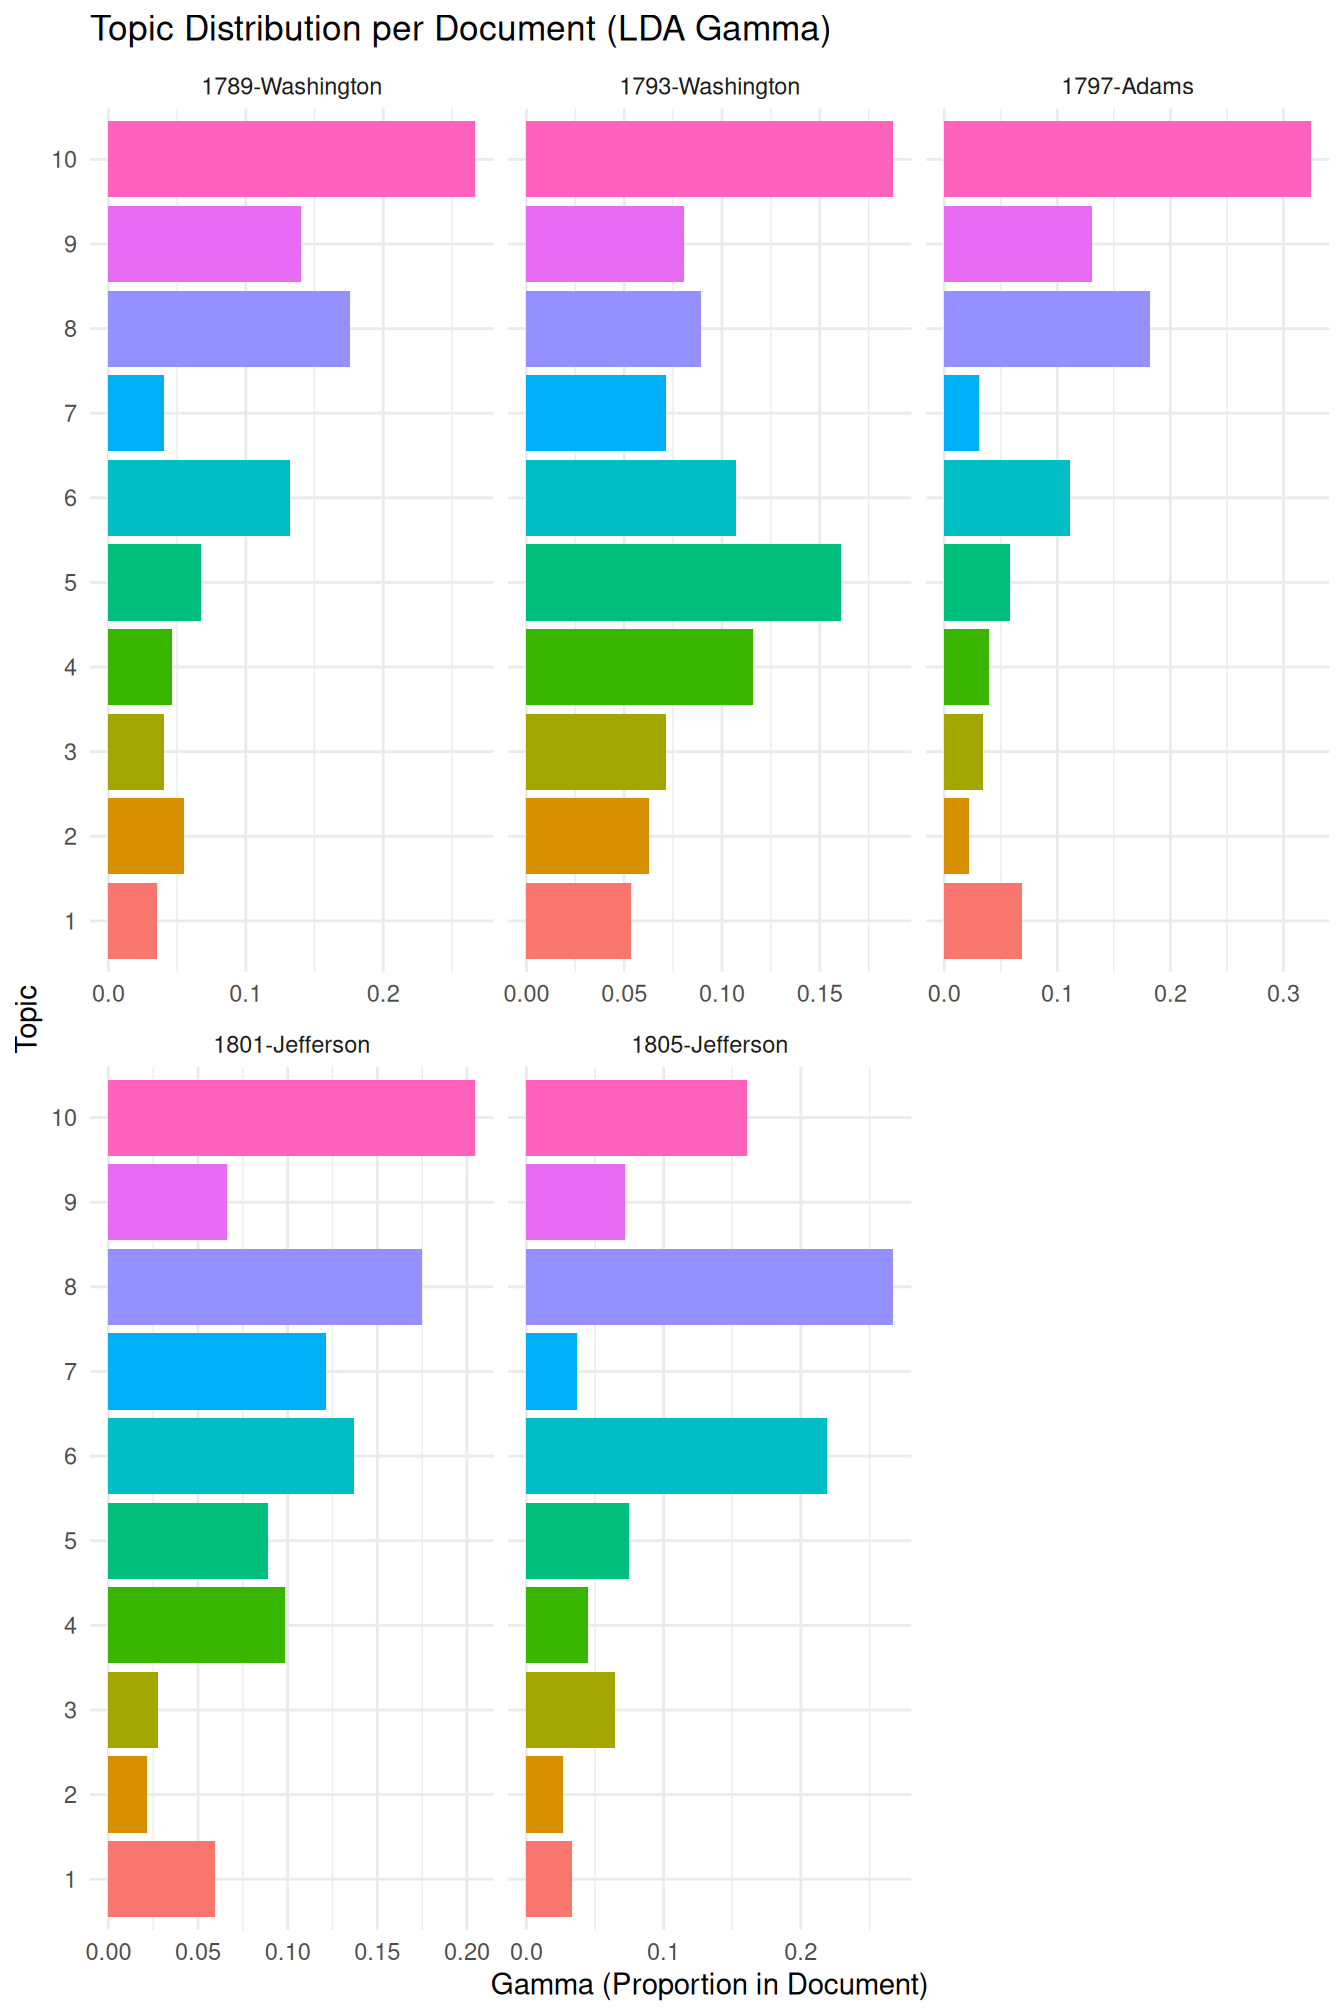
\includegraphics[keepaspectratio]{Introduction-to-Quantitative-Text-Analysis_files/figure-latex/lda-tidy-graph2-1.pdf}}

It might be a good idea at this point to refer back to the ``Validate, Validate,''Validate'' by Grimmer \& Stewart (\citeproc{ref-Grimmer2013a}{2013}), which we mentioned earlier. This is especially relevant here, as unsupervised methods literally ``find'' patterns, with the risk that --- given we tend to be very good at recognizing patterns -- we find non-sense patterns. Thus, we must ensure that the patterns or topics we find are meaningful and useful. The validation needed for this often involves a combination of quantitative metrics and qualitative interpretation.

On the quantitative side, we can use \textbf{topic coherence}, which assesses the semantic similarity between the high-scoring words in a topic. Topics with high coherence tend to be more human-interpretable. While the \texttt{topicmodels} package doesn't directly provide a built-in topic coherence measure, it can be computed using other packages like \texttt{ldatuning} or manual calculation based on word co-occurrence statistics in the corpus (we will return to this when discussing STM, where the package makes this significantly easier).

Another quantitative approach involves examining \textbf{perplexity}, a measure of how well the model predicts a held-out set of documents.
Lower perplexity generally indicates a better model fit. As the \texttt{topicmodels} package provides the log-likelihood of the model, we can derive the perplexity from it.

\begin{Shaded}
\begin{Highlighting}[]
\CommentTok{\# Get the log{-}likelihood of the fitted model}
\NormalTok{log\_likelihood }\OtherTok{\textless{}{-}} \FunctionTok{logLik}\NormalTok{(inaugural\_lda10)}
\NormalTok{N }\OtherTok{\textless{}{-}} \FunctionTok{sum}\NormalTok{(inaugural\_dtm)  }\CommentTok{\# Calculate the total words in the document{-}term matrix.}
\NormalTok{perplexity }\OtherTok{\textless{}{-}} \FunctionTok{exp}\NormalTok{(}\SpecialCharTok{{-}}\NormalTok{log\_likelihood}\SpecialCharTok{/}\NormalTok{N)  }\CommentTok{\# Calculate perplexity using the formula.}
\FunctionTok{print}\NormalTok{(}\FunctionTok{paste}\NormalTok{(}\StringTok{"Perplexity of the LDA model:"}\NormalTok{, perplexity))}
\end{Highlighting}
\end{Shaded}

\begin{verbatim}
## [1] "Perplexity of the LDA model: 1262.87536366491"
\end{verbatim}

Most importantly, beyond quantitative metrics, \textbf{qualitative evaluation} is essential. For LDA, this involves carefully inspecting the top terms for each topic (as shown in the beta visualization) and assessing whether they form a coherent theme. We also examine the document-topic distributions (gamma visualization) to see if documents with high proportions of a given topic are indeed about the interpreted theme. Comparing topic assignments to known characteristics of documents or human judgments (if available) can also provide valuable validation. Experimenting with different numbers of topics (\(k\)) and comparing the resulting topics qualitatively and quantitatively is a standard practice in LDA model validation.

Finally, the choice of the number of topics (\(k\)) is the most problematic aspect of validation as, while quantitative measures like coherence or perplexity can guide this choice, ultimately, the interpretability and utility of the topics for the research question are paramount. To compare models with different numbers of topics, one would typically train multiple LDA models (each with a different \(k\)) and then compare their log-likelihood/perplexity or topic coherence scores, visualizing these scores against \(k\).

\section{Seeded Latent Dirichlet Allocation (sLDA)}\label{seeded-latent-dirichlet-allocation-slda}

An alternative to the above approach is one known as seeded-LDA. This approach uses seed words to steer the LDA in the right direction. One origin of these seed words can be a dictionary that tells the algorithm which words belong together in various categories. To use it, we will first load the packages and set a seed:

\begin{Shaded}
\begin{Highlighting}[]
\FunctionTok{library}\NormalTok{(seededlda)}
\FunctionTok{library}\NormalTok{(quanteda.dictionaries)}

\FunctionTok{set.seed}\NormalTok{(}\DecValTok{42}\NormalTok{)}
\end{Highlighting}
\end{Shaded}

Next, we need to specify a selection of seed words in dictionary form. While we can construct a dictionary ourselves, we use the Laver and Garry dictionary we saw earlier. We then use this dictionary to run our seeded LDA:

\begin{Shaded}
\begin{Highlighting}[]
\NormalTok{dictionary\_LaverGarry }\OtherTok{\textless{}{-}} \FunctionTok{dictionary}\NormalTok{(data\_dictionary\_LaverGarry)}
\NormalTok{seededmodel }\OtherTok{\textless{}{-}} \FunctionTok{textmodel\_seededlda}\NormalTok{(data\_inaugural\_dfm, }\AttributeTok{dictionary =}\NormalTok{ dictionary\_LaverGarry)}
\end{Highlighting}
\end{Shaded}

Note that using the dictionary has ensured that we only use the categories in the dictionary. This means we can look at which topics are in each inaugural speech and which terms were most likely for each. Let us start with the topics first:

\begin{Shaded}
\begin{Highlighting}[]
\NormalTok{topics }\OtherTok{\textless{}{-}} \FunctionTok{topics}\NormalTok{(seededmodel)}
\NormalTok{topics\_table }\OtherTok{\textless{}{-}} \FunctionTok{ftable}\NormalTok{(topics)}
\NormalTok{topics\_prop\_table }\OtherTok{\textless{}{-}} \FunctionTok{as.data.frame}\NormalTok{(}\FunctionTok{prop.table}\NormalTok{(topics\_table))}

\FunctionTok{ggplot}\NormalTok{(}\AttributeTok{data =}\NormalTok{ topics\_prop\_table, }\FunctionTok{aes}\NormalTok{(}\AttributeTok{x =}\NormalTok{ topics, }\AttributeTok{y =}\NormalTok{ Freq)) }\SpecialCharTok{+} \FunctionTok{geom\_bar}\NormalTok{(}\AttributeTok{stat =} \StringTok{"identity"}\NormalTok{) }\SpecialCharTok{+}
    \FunctionTok{labs}\NormalTok{(}\AttributeTok{x =} \StringTok{"Topics"}\NormalTok{, }\AttributeTok{y =} \StringTok{"Topic Percentage"}\NormalTok{) }\SpecialCharTok{+} \FunctionTok{scale\_y\_continuous}\NormalTok{(}\AttributeTok{expand =} \FunctionTok{c}\NormalTok{(}\DecValTok{0}\NormalTok{,}
    \DecValTok{0}\NormalTok{)) }\SpecialCharTok{+} \FunctionTok{theme\_classic}\NormalTok{() }\SpecialCharTok{+} \FunctionTok{theme}\NormalTok{(}\AttributeTok{axis.text.x =} \FunctionTok{element\_text}\NormalTok{(}\AttributeTok{size =} \DecValTok{10}\NormalTok{, }\AttributeTok{angle =} \DecValTok{90}\NormalTok{,}
    \AttributeTok{hjust =} \DecValTok{1}\NormalTok{))}
\end{Highlighting}
\end{Shaded}

\pandocbounded{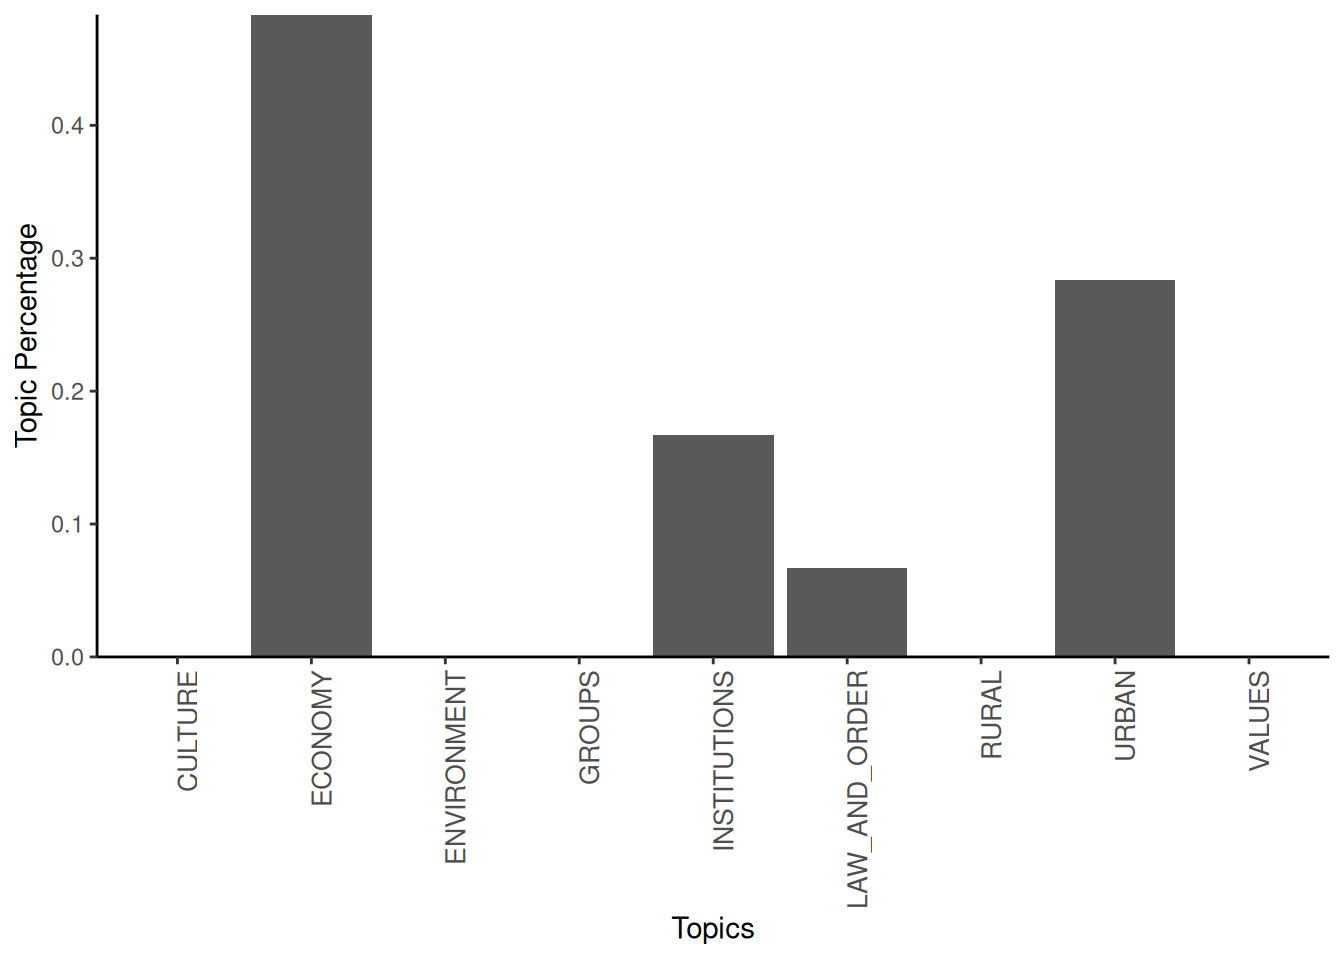
\includegraphics[keepaspectratio]{Introduction-to-Quantitative-Text-Analysis_files/figure-latex/ggplot-seededlda-1.pdf}}

Here, we find that Culture was the most favoured topic, followed by the Economy and Values. Finally, we can then have a look at the most likely terms for each topic, sorted by each of the categories in the dictionary:

\begin{Shaded}
\begin{Highlighting}[]
\NormalTok{terms }\OtherTok{\textless{}{-}} \FunctionTok{terms}\NormalTok{(seededmodel)}
\NormalTok{terms\_table }\OtherTok{\textless{}{-}} \FunctionTok{ftable}\NormalTok{(terms)}
\NormalTok{terms\_df }\OtherTok{\textless{}{-}} \FunctionTok{as.data.frame}\NormalTok{(terms\_table)}
\FunctionTok{head}\NormalTok{(terms\_df)}
\end{Highlighting}
\end{Shaded}

\begin{verbatim}
##   Var1    Var2      Freq
## 1    A CULTURE    people
## 2    B CULTURE   demands
## 3    C CULTURE operation
## 4    D CULTURE      idea
## 5    E CULTURE     lines
## 6    F CULTURE     price
\end{verbatim}

Here, we find that in the first cluster (denoted as `A'), the word `people' was most likely (from all words that belonged to Culture). Thus, within this cluster, talking about culture often references the people. In the same way, we can make similar observations for the other categories.

\section{Structural Topic Model (STM)}\label{structural-topic-model-stm}

The Structural Topic Model (STM) is another probabilistic topic modelling approach that extends traditional LDA by explicitly incorporating document metadata (such as publication date, author, source, or other document-level characteristics) into the model.
STM can model:

\begin{enumerate}
\def\labelenumi{\arabic{enumi}.}
\tightlist
\item
  \textbf{Topic prevalence:} How the proportion of topics in a document relates to metadata. For example, how does the prevalence of ``business'' topics change over time or differ between authors?
\item
  \textbf{Topic content:} How the words associated with a topic (the \(\beta\) distribution) vary according to metadata. For example, are the words used to discuss ``the environment'' different in documents from different political parties?
\end{enumerate}

One of the key advantages of STM is that it uses this metadata to estimate the topic-document (\(\theta\)) and topic-word (\(\beta\)) distributions, potentially leading to more coherent and meaningful topics and allowing researchers to directly test hypotheses about the relationship between metadata and language use. Also, Unlike standard LDA, where the hyperparameters (\(\alpha\) and \(\beta\)) are typically fixed, STM allows them to be influenced by covariates.

Figure \ref{fig:stm-diagram} provides a diagram illustrating the structure of the STM.

\hfill\break

\begin{figure}
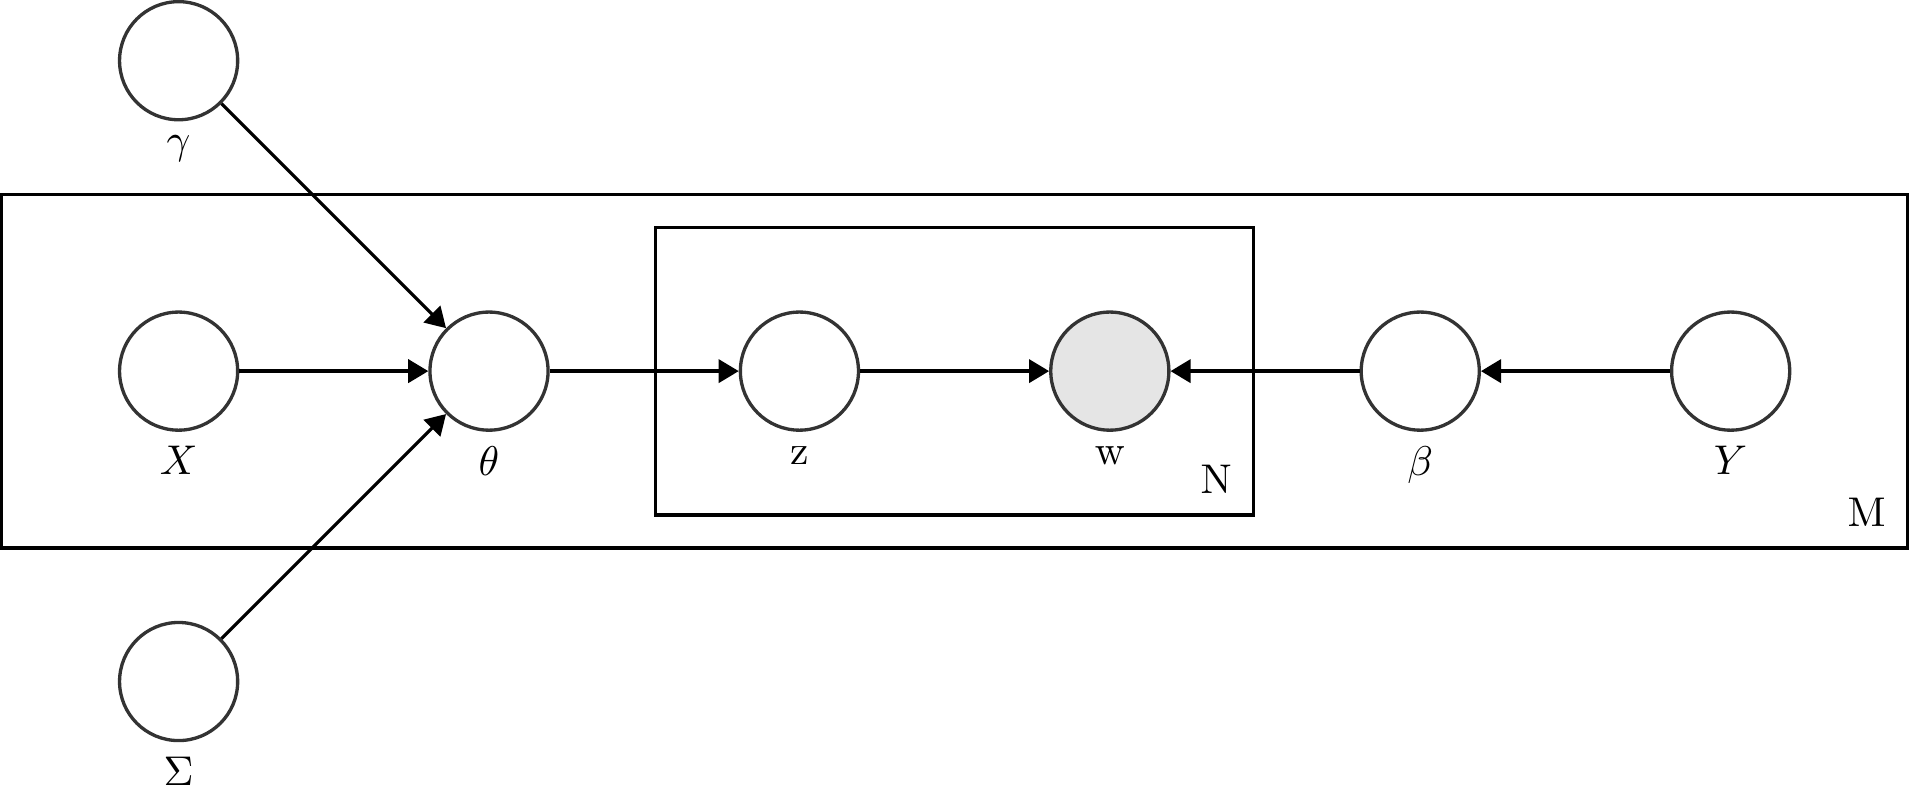
\includegraphics[width=0.9\linewidth]{Introduction-to-Quantitative-Text-Analysis_files/figure-latex/stm-diagram-1} \caption{Plate diagram for a Structucal Topic Model.}\label{fig:stm-diagram}
\end{figure}

\hfill\break

Figure \ref{fig:stm-diagram} shows stm in the form of a plate diagram. Here, \(X\) refers to the prevalence metadata; \(\gamma\), the metadata weights; \(\Sigma\), the topic covariances; \(\theta\), the document prevalence; \(z\), the per-word topic; \(w\), the observed word; \(Y\), the content metadata; \(\beta\), the topic content; \(N\), the number of words in a document; and \(M\), the number of documents in the corpus.

To run stm in R, we have to load the package, set a seed, convert our dfm to the stm format and place our documents, vocabulary (the tokens) and any other data in three separate objects (for later convenience):

\begin{Shaded}
\begin{Highlighting}[]
\FunctionTok{library}\NormalTok{(stm)}
\FunctionTok{library}\NormalTok{(quanteda)}

\FunctionTok{set.seed}\NormalTok{(}\DecValTok{42}\NormalTok{)}

\NormalTok{data\_inaugural\_stm }\OtherTok{\textless{}{-}} \FunctionTok{convert}\NormalTok{(data\_inaugural\_dfm, }\AttributeTok{to =} \StringTok{"stm"}\NormalTok{)}

\NormalTok{documents }\OtherTok{\textless{}{-}}\NormalTok{ data\_inaugural\_stm}\SpecialCharTok{$}\NormalTok{documents}
\NormalTok{vocabulary }\OtherTok{\textless{}{-}}\NormalTok{ data\_inaugural\_stm}\SpecialCharTok{$}\NormalTok{vocab}
\NormalTok{meta }\OtherTok{\textless{}{-}}\NormalTok{ data\_inaugural\_stm}\SpecialCharTok{$}\NormalTok{meta}
\end{Highlighting}
\end{Shaded}

The first thing we have to do is find the number of topics we need. In the \texttt{stm} package, we can do this by using a function called \texttt{searchK}. Here, we specify a range of values that could include the `correct' number of topics, which we then run and collect. Afterwards, we then look at several goodness-of-fit measures to assess which number of topics (which \emph{k}) has the best fit for the data. These measures include exclusivity, semantic coherence, held-out likelihood, bound, lbound, and residual dispersion. Here, we run this for 2 to 15 possible topics.

In our code, we specify our documents, our tokens (the vocabulary), and our meta-data. Moreover, as our prevalence, we include parameters for \texttt{Year} and \texttt{Party}, as we expect the content of the topics to differ between both the Republican and Democratic party, as well as over time:

\begin{Shaded}
\begin{Highlighting}[]
\NormalTok{k }\OtherTok{\textless{}{-}} \FunctionTok{c}\NormalTok{(}\DecValTok{3}\NormalTok{, }\DecValTok{4}\NormalTok{, }\DecValTok{5}\NormalTok{, }\DecValTok{6}\NormalTok{, }\DecValTok{7}\NormalTok{, }\DecValTok{8}\NormalTok{, }\DecValTok{9}\NormalTok{, }\DecValTok{10}\NormalTok{, }\DecValTok{11}\NormalTok{, }\DecValTok{12}\NormalTok{, }\DecValTok{13}\NormalTok{, }\DecValTok{14}\NormalTok{, }\DecValTok{15}\NormalTok{)}
\end{Highlighting}
\end{Shaded}

\begin{Shaded}
\begin{Highlighting}[]
\NormalTok{findingk }\OtherTok{\textless{}{-}} \FunctionTok{searchK}\NormalTok{(documents, vocabulary, k, }\AttributeTok{prevalence =} \SpecialCharTok{\textasciitilde{}}\NormalTok{Party }\SpecialCharTok{+} \FunctionTok{s}\NormalTok{(Year), }\AttributeTok{data =}\NormalTok{ meta,}
    \AttributeTok{verbose =} \ConstantTok{TRUE}\NormalTok{)}
\end{Highlighting}
\end{Shaded}

\begin{Shaded}
\begin{Highlighting}[]
\NormalTok{findingk\_results }\OtherTok{\textless{}{-}} \FunctionTok{as.data.frame}\NormalTok{(}\FunctionTok{matrix}\NormalTok{(}\FunctionTok{unlist}\NormalTok{(findingk}\SpecialCharTok{$}\NormalTok{results), }\AttributeTok{nrow =} \FunctionTok{length}\NormalTok{(}\FunctionTok{unlist}\NormalTok{(findingk}\SpecialCharTok{$}\NormalTok{results[}\DecValTok{1}\NormalTok{]))))}
\NormalTok{names }\OtherTok{\textless{}{-}} \FunctionTok{names}\NormalTok{(findingk}\SpecialCharTok{$}\NormalTok{results)}
\FunctionTok{names}\NormalTok{(findingk\_results) }\OtherTok{\textless{}{-}}\NormalTok{ names}
\end{Highlighting}
\end{Shaded}

Looking at \texttt{findingk\_results} we find various values. The first, exclusivity, refers to the occurrence that when words have a high probability under one topic, they have a low probability under others. Related to this is semantic coherence which happens when the most probable words in a topic should occur in the same document. Held-out (or held-out log-likelihood) is the likelihood of our model on data that was not used in the initial estimation (the lower the better), while residuals refer to the difference between a data point and the mean value that the model predicts for that data point (which we want to be 1, indicating a standard distribution). Finally, bound and lbound refer to a model's internal measure of fit. Here, we will be looking for the number of topics, that balance the exclusivity and the semantic coherence, have a residual around 1, and a low held-out. To make this simpler, we visualise our data. In the first graph we plot all the values, while in the second, we only look at the exclusivity and the semantic coherence (as they are the most important):

\begin{Shaded}
\begin{Highlighting}[]
\FunctionTok{library}\NormalTok{(reshape2)}

\NormalTok{findingk\_melt }\OtherTok{\textless{}{-}} \FunctionTok{melt}\NormalTok{(findingk\_results, }\AttributeTok{id =} \StringTok{"K"}\NormalTok{)}
\NormalTok{findingk\_melt}\SpecialCharTok{$}\NormalTok{variable }\OtherTok{\textless{}{-}} \FunctionTok{as.character}\NormalTok{(findingk\_melt}\SpecialCharTok{$}\NormalTok{variable)}
\NormalTok{findingk}\SpecialCharTok{$}\NormalTok{K }\OtherTok{\textless{}{-}} \FunctionTok{as.factor}\NormalTok{(findingk\_results}\SpecialCharTok{$}\NormalTok{K)}

\FunctionTok{ggplot}\NormalTok{(findingk\_melt, }\FunctionTok{aes}\NormalTok{(K, value)) }\SpecialCharTok{+} \FunctionTok{geom\_point}\NormalTok{() }\SpecialCharTok{+} \FunctionTok{geom\_line}\NormalTok{() }\SpecialCharTok{+} \FunctionTok{facet\_wrap}\NormalTok{(}\SpecialCharTok{\textasciitilde{}}\NormalTok{variable,}
    \AttributeTok{scales =} \StringTok{"free"}\NormalTok{) }\SpecialCharTok{+} \FunctionTok{theme\_classic}\NormalTok{()}
\end{Highlighting}
\end{Shaded}

\pandocbounded{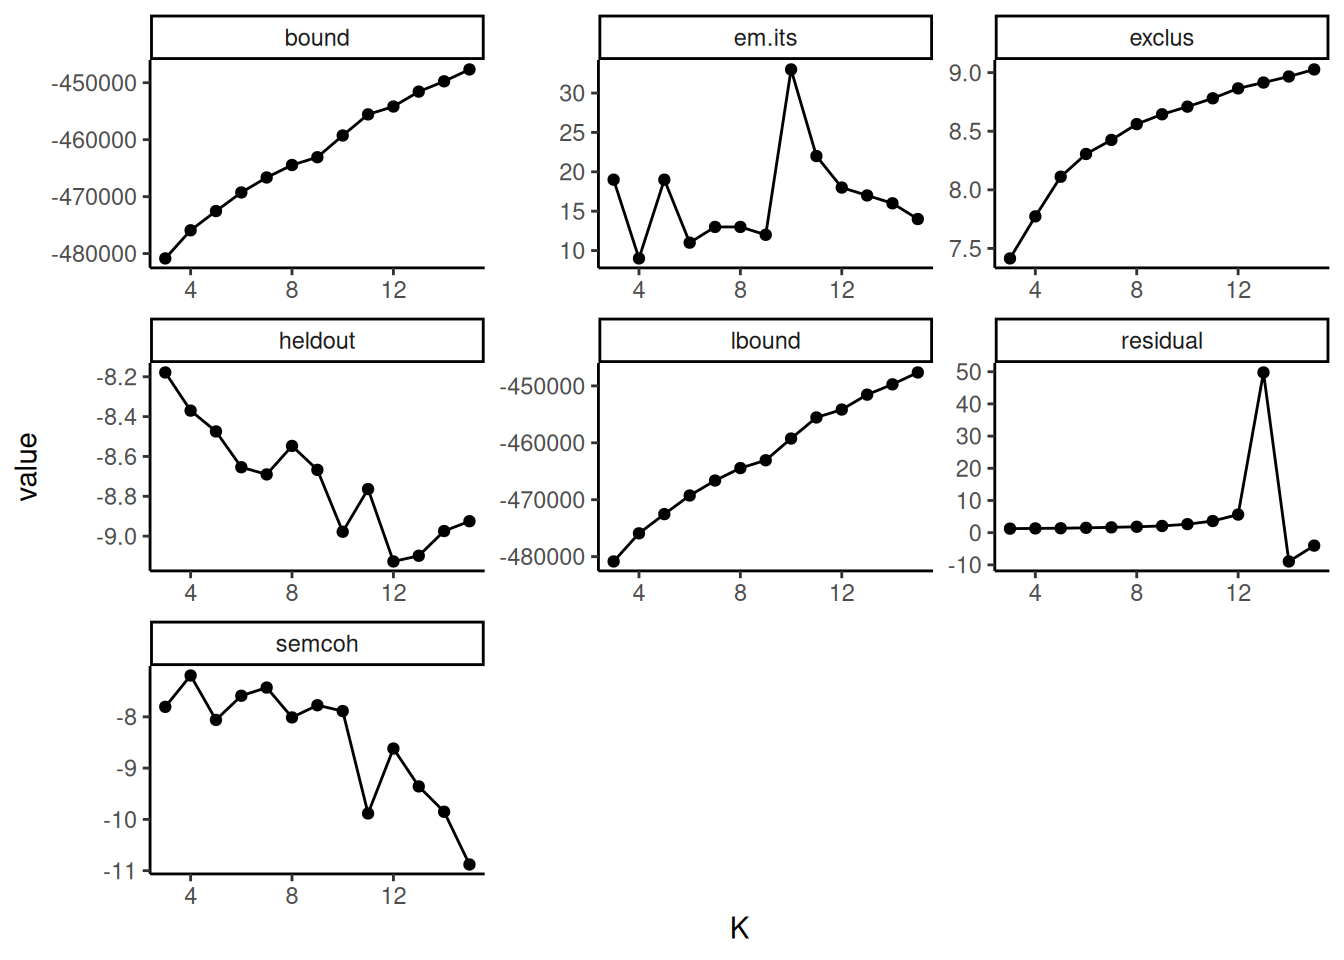
\includegraphics[keepaspectratio]{Introduction-to-Quantitative-Text-Analysis_files/figure-latex/ggplot-stm-findk-1.pdf}}

\begin{Shaded}
\begin{Highlighting}[]
\FunctionTok{ggplot}\NormalTok{(findingk\_results, }\FunctionTok{aes}\NormalTok{(semcoh, exclus)) }\SpecialCharTok{+} \FunctionTok{geom\_point}\NormalTok{() }\SpecialCharTok{+} \FunctionTok{geom\_text}\NormalTok{(}\AttributeTok{data =}\NormalTok{ findingk\_results,}
    \AttributeTok{label =}\NormalTok{ findingk}\SpecialCharTok{$}\NormalTok{K, }\AttributeTok{nudge\_x =} \FloatTok{0.15}\NormalTok{) }\SpecialCharTok{+} \FunctionTok{scale\_x\_continuous}\NormalTok{(}\StringTok{"Semantic Coherence"}\NormalTok{) }\SpecialCharTok{+}
    \FunctionTok{scale\_y\_continuous}\NormalTok{(}\StringTok{"Exclusivity"}\NormalTok{) }\SpecialCharTok{+} \FunctionTok{theme\_classic}\NormalTok{()}
\end{Highlighting}
\end{Shaded}

\pandocbounded{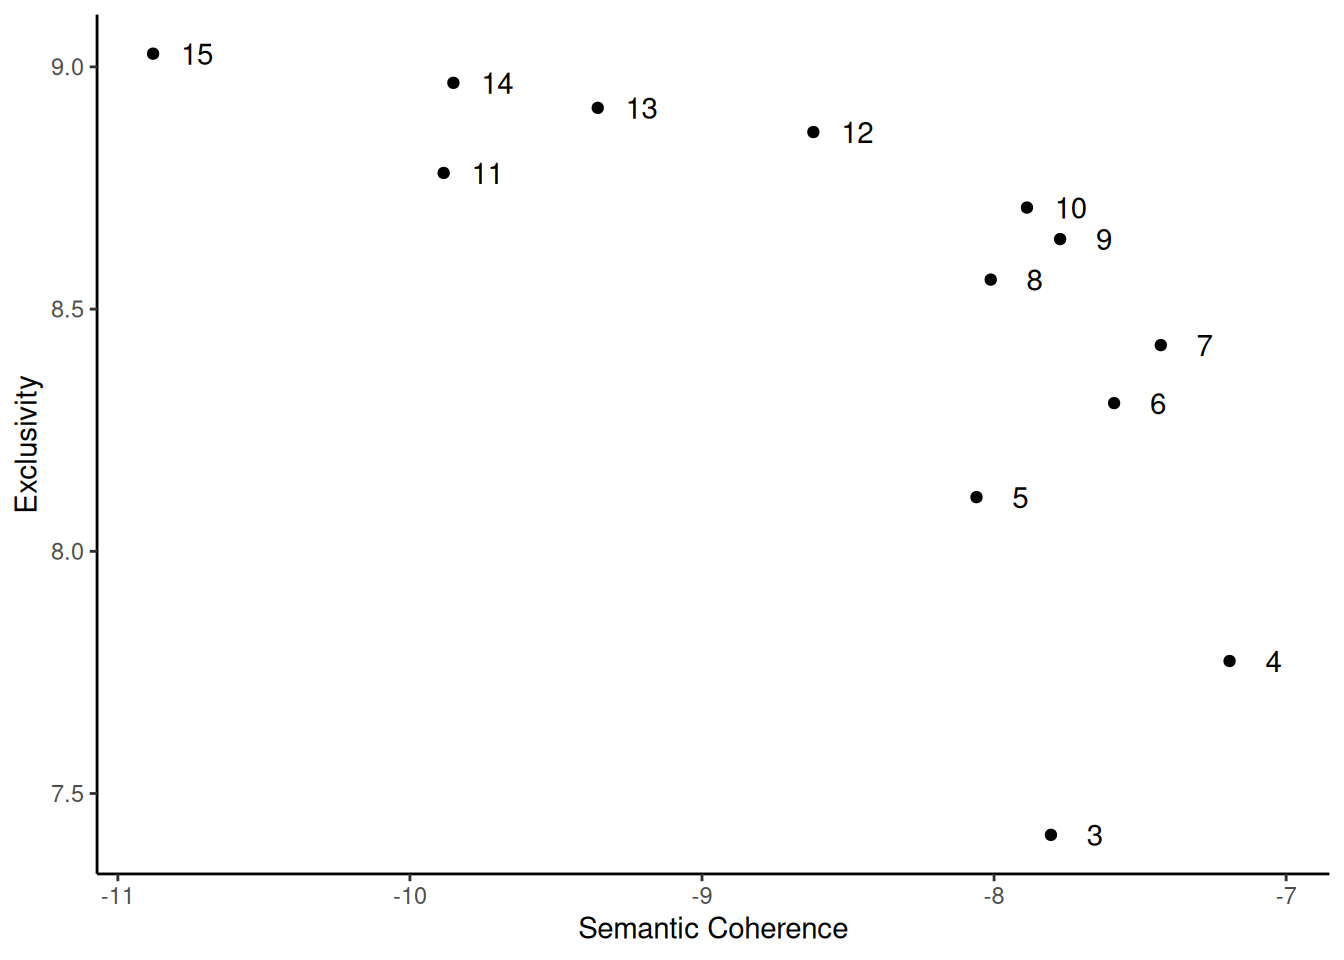
\includegraphics[keepaspectratio]{Introduction-to-Quantitative-Text-Analysis_files/figure-latex/ggplot-stm-findk-2.pdf}}

Based on these graphs, we decide upon 10 topics. The main reason for this is that for this number of topics, there is a high semantic coherence given the exclusivity. We can now run our stm model, using spectral initialization and a topical prevalence including both the Party and the Year of the inauguration. Also, we have a look at the topics, and the words with the highest probability attached to them:

\begin{Shaded}
\begin{Highlighting}[]
\NormalTok{n\_topics }\OtherTok{\textless{}{-}} \DecValTok{10}
\NormalTok{output\_stm }\OtherTok{\textless{}{-}} \FunctionTok{stm}\NormalTok{(documents, vocabulary, }\AttributeTok{K =}\NormalTok{ n\_topics, }\AttributeTok{prevalence =} \SpecialCharTok{\textasciitilde{}}\NormalTok{Party }\SpecialCharTok{+} \FunctionTok{s}\NormalTok{(Year),}
    \AttributeTok{data =}\NormalTok{ meta, }\AttributeTok{init.type =} \StringTok{"Spectral"}\NormalTok{, }\AttributeTok{verbose =} \ConstantTok{TRUE}\NormalTok{)}
\FunctionTok{labelTopics}\NormalTok{(output\_stm)}
\end{Highlighting}
\end{Shaded}

Here, we see that the word \texttt{us} is dominant in most topics, making it a candidate for removal as a stop word in a future analysis. Looking closer, we find that the first topic refers to peace, the second, third and seventh to the world, the fourth and sixth to America, and the eighth to the government.

Finally, we can see whether there is any relation between these topics and any of the parameters we included. Here, let us look at any existing differences between the two parties:

\begin{Shaded}
\begin{Highlighting}[]
\NormalTok{est\_assoc\_effect }\OtherTok{\textless{}{-}} \FunctionTok{estimateEffect}\NormalTok{(}\SpecialCharTok{\textasciitilde{}}\NormalTok{Party, output\_stm, }\AttributeTok{metadata =}\NormalTok{ meta, }\AttributeTok{prior =} \FloatTok{1e{-}05}\NormalTok{)}
\end{Highlighting}
\end{Shaded}

While we can visualise this with the \texttt{plot.estimateEffect} option, the visualisation is far from ideal. Thus, let us use some data-wrangling and make the plot ourselves:

\begin{Shaded}
\begin{Highlighting}[]
\NormalTok{estimate\_data }\OtherTok{\textless{}{-}} \FunctionTok{plot.estimateEffect}\NormalTok{(est\_assoc\_effect, }\StringTok{"Party"}\NormalTok{, }\AttributeTok{method =} \StringTok{"pointestimate"}\NormalTok{,}
    \AttributeTok{model =}\NormalTok{ output\_stm, }\AttributeTok{omit.plot =} \ConstantTok{TRUE}\NormalTok{)}
\NormalTok{estimate\_graph\_means }\OtherTok{\textless{}{-}}\NormalTok{ estimate\_data}\SpecialCharTok{$}\NormalTok{means}
\NormalTok{estimate\_graph\_means }\OtherTok{\textless{}{-}} \FunctionTok{data.frame}\NormalTok{(}\FunctionTok{matrix}\NormalTok{(}\FunctionTok{unlist}\NormalTok{(estimate\_graph\_means), }\AttributeTok{nrow =} \FunctionTok{length}\NormalTok{(estimate\_graph\_means),}
    \AttributeTok{byrow =} \ConstantTok{TRUE}\NormalTok{))}
\NormalTok{estimate\_graph\_means }\OtherTok{\textless{}{-}} \FunctionTok{data.frame}\NormalTok{(}\FunctionTok{c}\NormalTok{(}\FunctionTok{rep}\NormalTok{(}\StringTok{"Republicans"}\NormalTok{, }\DecValTok{10}\NormalTok{), }\FunctionTok{rep}\NormalTok{(}\StringTok{"Democrats"}\NormalTok{, }\DecValTok{10}\NormalTok{)),}
    \FunctionTok{c}\NormalTok{(estimate\_graph\_means}\SpecialCharTok{$}\NormalTok{X1, estimate\_graph\_means}\SpecialCharTok{$}\NormalTok{X2))}

\NormalTok{estimate\_graph\_cis }\OtherTok{\textless{}{-}}\NormalTok{ estimate\_data}\SpecialCharTok{$}\NormalTok{cis}
\NormalTok{estimate\_graph\_cis }\OtherTok{\textless{}{-}} \FunctionTok{data.frame}\NormalTok{(}\FunctionTok{matrix}\NormalTok{(}\FunctionTok{unlist}\NormalTok{(estimate\_graph\_cis), }\AttributeTok{nrow =} \FunctionTok{length}\NormalTok{(estimate\_graph\_cis),}
    \AttributeTok{byrow =} \ConstantTok{TRUE}\NormalTok{))}
\NormalTok{estimate\_graph\_cis }\OtherTok{\textless{}{-}} \FunctionTok{data.frame}\NormalTok{(}\FunctionTok{c}\NormalTok{(estimate\_graph\_cis}\SpecialCharTok{$}\NormalTok{X1, estimate\_graph\_cis}\SpecialCharTok{$}\NormalTok{X3),}
    \FunctionTok{c}\NormalTok{(estimate\_graph\_cis}\SpecialCharTok{$}\NormalTok{X2, estimate\_graph\_cis}\SpecialCharTok{$}\NormalTok{X4))}

\NormalTok{Topic }\OtherTok{\textless{}{-}} \FunctionTok{c}\NormalTok{(}\StringTok{"Topic 1"}\NormalTok{, }\StringTok{"Topic 2"}\NormalTok{, }\StringTok{"Topic 3"}\NormalTok{, }\StringTok{"Topic 4"}\NormalTok{, }\StringTok{"Topic 5"}\NormalTok{, }\StringTok{"Topic 6"}\NormalTok{, }\StringTok{"Topic 7"}\NormalTok{,}
    \StringTok{"Topic 8"}\NormalTok{, }\StringTok{"Topic 9"}\NormalTok{, }\StringTok{"Topic 10"}\NormalTok{, }\StringTok{"Topic 1"}\NormalTok{, }\StringTok{"Topic 2"}\NormalTok{, }\StringTok{"Topic 3"}\NormalTok{, }\StringTok{"Topic 4"}\NormalTok{,}
    \StringTok{"Topic 5"}\NormalTok{, }\StringTok{"Topic 6"}\NormalTok{, }\StringTok{"Topic 7"}\NormalTok{, }\StringTok{"Topic 8"}\NormalTok{, }\StringTok{"Topic 9"}\NormalTok{, }\StringTok{"Topic 10"}\NormalTok{)}

\NormalTok{estimate\_graph }\OtherTok{\textless{}{-}} \FunctionTok{cbind}\NormalTok{(Topic, estimate\_graph\_means, estimate\_graph\_cis)}
\FunctionTok{names}\NormalTok{(estimate\_graph) }\OtherTok{\textless{}{-}} \FunctionTok{c}\NormalTok{(}\StringTok{"Topic"}\NormalTok{, }\StringTok{"Party"}\NormalTok{, }\StringTok{"Mean"}\NormalTok{, }\StringTok{"min"}\NormalTok{, }\StringTok{"max"}\NormalTok{)}
\NormalTok{estimate\_graph}\SpecialCharTok{$}\NormalTok{Party }\OtherTok{\textless{}{-}} \FunctionTok{as.factor}\NormalTok{(estimate\_graph}\SpecialCharTok{$}\NormalTok{Party)}
\NormalTok{estimate\_graph}\SpecialCharTok{$}\NormalTok{Topic }\OtherTok{\textless{}{-}} \FunctionTok{as.factor}\NormalTok{(estimate\_graph}\SpecialCharTok{$}\NormalTok{Topic)}
\NormalTok{estimate\_graph}\SpecialCharTok{$}\NormalTok{Topic }\OtherTok{\textless{}{-}} \FunctionTok{factor}\NormalTok{(estimate\_graph}\SpecialCharTok{$}\NormalTok{Topic, }\AttributeTok{levels =} \FunctionTok{rev}\NormalTok{(}\FunctionTok{levels}\NormalTok{(estimate\_graph}\SpecialCharTok{$}\NormalTok{Topic)))}
\end{Highlighting}
\end{Shaded}

Now, let us plot our intervals:

\begin{Shaded}
\begin{Highlighting}[]
\FunctionTok{ggplot}\NormalTok{(estimate\_graph, }\FunctionTok{aes}\NormalTok{(Mean, Topic)) }\SpecialCharTok{+} \FunctionTok{geom\_pointrange}\NormalTok{(}\FunctionTok{aes}\NormalTok{(}\AttributeTok{xmin =}\NormalTok{ min, }\AttributeTok{xmax =}\NormalTok{ max,}
    \AttributeTok{color =}\NormalTok{ Party), }\AttributeTok{position =} \FunctionTok{position\_dodge}\NormalTok{(}\FloatTok{0.3}\NormalTok{)) }\SpecialCharTok{+} \FunctionTok{geom\_vline}\NormalTok{(}\AttributeTok{xintercept =} \DecValTok{0}\NormalTok{,}
    \AttributeTok{linetype =} \StringTok{"dashed"}\NormalTok{, }\AttributeTok{size =} \FloatTok{0.5}\NormalTok{) }\SpecialCharTok{+} \FunctionTok{scale\_color\_manual}\NormalTok{(}\AttributeTok{values =} \FunctionTok{c}\NormalTok{(}\StringTok{"\#0015BC"}\NormalTok{, }\StringTok{"\#E9141D"}\NormalTok{)) }\SpecialCharTok{+}
    \FunctionTok{theme\_classic}\NormalTok{()}
\end{Highlighting}
\end{Shaded}

\begin{verbatim}
## Warning: Using `size` aesthetic for lines was deprecated in ggplot2 3.4.0.
## i Please use `linewidth` instead.
## This warning is displayed once every 8 hours.
## Call `lifecycle::last_lifecycle_warnings()` to see where this warning
## was generated.
\end{verbatim}

\pandocbounded{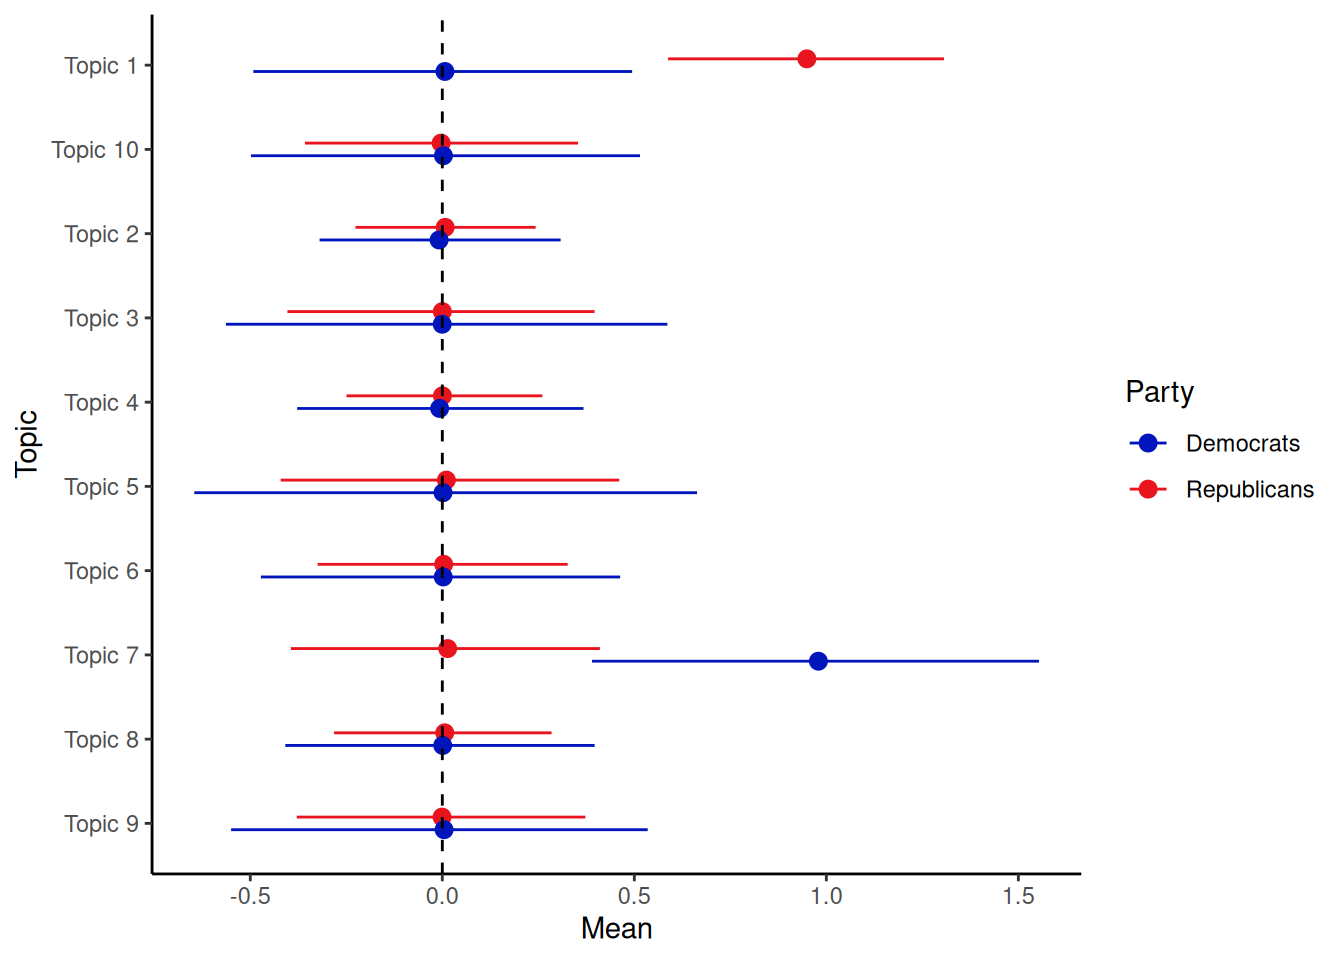
\includegraphics[keepaspectratio]{Introduction-to-Quantitative-Text-Analysis_files/figure-latex/ggplot-stm-intervals-1.pdf}}

Here, we find that while the averages for the topic do seem to differ a little between both of the parties, all the intervals are overlapping, indicating that they are not that different.

\section{Latent Semantic Analysis (LSA)}\label{latent-semantic-analysis-lsa}

Finally, we will look at Latent Semantic Analysis (LSA), a matrix factorization technique that uses Singular Value Decomposition (SVD) on a term-document matrix to uncover latent semantic structures. Unlike probabilistic models like LDA or STM, LSA is algebraic and assumes that semantically similar terms appear in similar documents.

We'll use the \texttt{textmodel\_lsa()} function from the \texttt{quanteda.textmodels} package to perform LSA on the U.S. Presidential Inaugural Corpus.

Before applying LSA, we need to load the necessary R libraries and prepare the text data:

\begin{Shaded}
\begin{Highlighting}[]
\FunctionTok{library}\NormalTok{(quanteda)}
\FunctionTok{library}\NormalTok{(quanteda.textmodels)}
\FunctionTok{library}\NormalTok{(dplyr)}
\FunctionTok{library}\NormalTok{(tidyr)}
\FunctionTok{library}\NormalTok{(ggplot2)}

\FunctionTok{data}\NormalTok{(}\StringTok{"data\_corpus\_inaugural"}\NormalTok{)}

\NormalTok{inaugural\_tokens }\OtherTok{\textless{}{-}} \FunctionTok{tokens}\NormalTok{(data\_corpus\_inaugural, }\AttributeTok{remove\_punct =} \ConstantTok{TRUE}\NormalTok{, }\AttributeTok{remove\_symbols =} \ConstantTok{TRUE}\NormalTok{,}
    \AttributeTok{remove\_numbers =} \ConstantTok{TRUE}\NormalTok{) }\SpecialCharTok{\%\textgreater{}\%}
    \FunctionTok{tokens\_tolower}\NormalTok{() }\SpecialCharTok{\%\textgreater{}\%}
    \FunctionTok{tokens\_remove}\NormalTok{(}\FunctionTok{stopwords}\NormalTok{(}\StringTok{"en"}\NormalTok{))}

\NormalTok{inaugural\_dfm }\OtherTok{\textless{}{-}} \FunctionTok{dfm}\NormalTok{(inaugural\_tokens)}
\end{Highlighting}
\end{Shaded}

With the data preprocessed and organized into a document-feature matrix, we are ready to fit the LSA model. We use the \texttt{textmodel\_lsa()} function, specifying the document-feature matrix and the desired number of latent dimensions (\texttt{nd}). Again, choosing the optimal number of dimensions often requires experimentation and evaluation, which we will look at in the validation section. Setting a random seed ensures that the results are reproducible.

\begin{Shaded}
\begin{Highlighting}[]
\FunctionTok{set.seed}\NormalTok{(}\DecValTok{42}\NormalTok{)}

\CommentTok{\# Fit LSA with 10 dimensions. The number of dimensions (nd) determines the size}
\CommentTok{\# of the reduced semantic space.}
\NormalTok{n\_dims }\OtherTok{\textless{}{-}} \DecValTok{10}
\NormalTok{lsa\_model }\OtherTok{\textless{}{-}} \FunctionTok{textmodel\_lsa}\NormalTok{(inaugural\_dfm, }\AttributeTok{nd =}\NormalTok{ n\_dims)}

\NormalTok{lsa\_model}
\end{Highlighting}
\end{Shaded}

\begin{verbatim}
##   [[ suppressing 33 column names 'fellow-citizens', 'senate', 'house' ... ]]
\end{verbatim}

After fitting the LSA model, we can explore the term loadings. Term loadings indicate the association of each term (word) with each of the discovered latent dimensions. High positive or negative loadings suggest that a term is strongly associated with a particular dimension. By examining the terms with the highest absolute loadings for each dimension, we can begin to interpret the semantic meaning captured by that dimension. We extract the term loadings from the model, convert them into a tidy data frame, and then identify the top terms for each dimension based on the absolute value of their loadings. Visualizing the top terms for a dimension, as shown in the optional plot, can aid in this interpretation.

\begin{Shaded}
\begin{Highlighting}[]
\NormalTok{term\_matrix }\OtherTok{\textless{}{-}} \FunctionTok{as.data.frame}\NormalTok{(lsa\_model}\SpecialCharTok{$}\NormalTok{features)}
\FunctionTok{colnames}\NormalTok{(term\_matrix) }\OtherTok{\textless{}{-}} \FunctionTok{paste0}\NormalTok{(}\StringTok{"Dim"}\NormalTok{, }\DecValTok{1}\SpecialCharTok{:}\NormalTok{n\_dims) }\CommentTok{\# Rename columns}
\NormalTok{term\_matrix}\SpecialCharTok{$}\NormalTok{term }\OtherTok{\textless{}{-}} \FunctionTok{rownames}\NormalTok{(term\_matrix) }\CommentTok{\# Add the actual terms as a column}

\NormalTok{term\_long }\OtherTok{\textless{}{-}}\NormalTok{ term\_matrix }\SpecialCharTok{\%\textgreater{}\%}
  \FunctionTok{pivot\_longer}\NormalTok{(}\AttributeTok{cols =} \FunctionTok{starts\_with}\NormalTok{(}\StringTok{"Dim"}\NormalTok{), }\AttributeTok{names\_to =} \StringTok{"Dimension"}\NormalTok{, }\AttributeTok{values\_to =} \StringTok{"Loading"}\NormalTok{)}

\NormalTok{top\_terms }\OtherTok{\textless{}{-}}\NormalTok{ term\_long }\SpecialCharTok{\%\textgreater{}\%}
  \FunctionTok{group\_by}\NormalTok{(Dimension) }\SpecialCharTok{\%\textgreater{}\%}
  \FunctionTok{slice\_max}\NormalTok{(}\FunctionTok{abs}\NormalTok{(Loading), }\AttributeTok{n =} \DecValTok{10}\NormalTok{, }\AttributeTok{with\_ties =} \ConstantTok{FALSE}\NormalTok{) }\SpecialCharTok{\%\textgreater{}\%} 
  \FunctionTok{arrange}\NormalTok{(Dimension, }\SpecialCharTok{{-}}\FunctionTok{abs}\NormalTok{(Loading))}

\FunctionTok{ggplot}\NormalTok{(}\FunctionTok{filter}\NormalTok{(top\_terms, Dimension }\SpecialCharTok{==} \StringTok{"Dim1"}\NormalTok{), }\FunctionTok{aes}\NormalTok{(}\AttributeTok{x =} \FunctionTok{reorder}\NormalTok{(term, Loading), }\AttributeTok{y =}\NormalTok{ Loading)) }\SpecialCharTok{+}
  \FunctionTok{geom\_col}\NormalTok{(}\AttributeTok{fill =} \StringTok{"steelblue"}\NormalTok{) }\SpecialCharTok{+} \CommentTok{\# Create a bar chart with the loading on the x{-}axis and term on the y{-}axis.}
  \FunctionTok{coord\_flip}\NormalTok{() }\SpecialCharTok{+} \CommentTok{\# Flip the coordinate axes to make term labels easier to read.}
  \FunctionTok{labs}\NormalTok{(}\AttributeTok{title =} \StringTok{"Top Terms for LSA Dimension 1"}\NormalTok{, }\AttributeTok{x =} \StringTok{"Term"}\NormalTok{, }\AttributeTok{y =} \StringTok{"Loading"}\NormalTok{) }\SpecialCharTok{+} \CommentTok{\# Add plot title and axis labels.}
  \FunctionTok{theme\_minimal}\NormalTok{() }\CommentTok{\# Use a minimal theme for a clean plot.}
\end{Highlighting}
\end{Shaded}

\pandocbounded{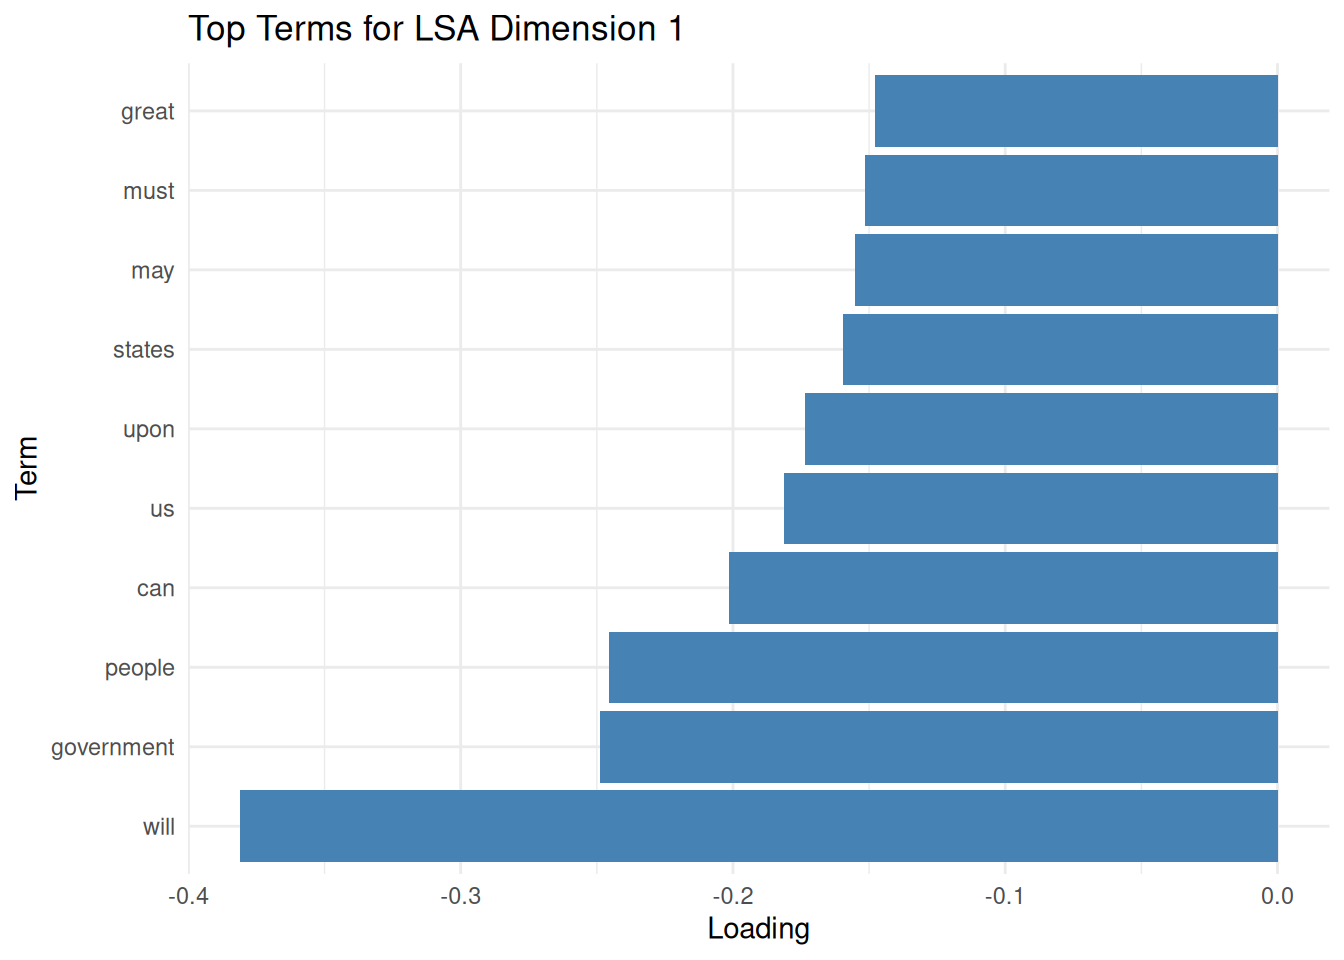
\includegraphics[keepaspectratio]{Introduction-to-Quantitative-Text-Analysis_files/figure-latex/lsa-terms-1.pdf}}

Similar to term loadings, we can explore document loadings. Document loadings represent the association of each document with each latent dimension. Documents with high positive or negative loadings on a particular dimension are estimated to be strongly related to the semantic concept captured by that dimension. By examining the documents with the highest loadings for each dimension, we can see which texts most represent the themes identified by LSA. We extract the document loadings and identify the top documents for each dimension based on their positive loadings.

\begin{Shaded}
\begin{Highlighting}[]
\NormalTok{doc\_matrix }\OtherTok{\textless{}{-}} \FunctionTok{as.data.frame}\NormalTok{(lsa\_model}\SpecialCharTok{$}\NormalTok{docs)}
\FunctionTok{colnames}\NormalTok{(doc\_matrix) }\OtherTok{\textless{}{-}} \FunctionTok{paste0}\NormalTok{(}\StringTok{"Dim"}\NormalTok{, }\DecValTok{1}\SpecialCharTok{:}\NormalTok{n\_dims) }
\NormalTok{doc\_matrix}\SpecialCharTok{$}\NormalTok{document }\OtherTok{\textless{}{-}} \FunctionTok{docnames}\NormalTok{(inaugural\_dfm) }

\NormalTok{doc\_long }\OtherTok{\textless{}{-}}\NormalTok{ doc\_matrix }\SpecialCharTok{\%\textgreater{}\%}
  \FunctionTok{pivot\_longer}\NormalTok{(}\AttributeTok{cols =} \FunctionTok{starts\_with}\NormalTok{(}\StringTok{"Dim"}\NormalTok{), }\AttributeTok{names\_to =} \StringTok{"Dimension"}\NormalTok{, }\AttributeTok{values\_to =} \StringTok{"Loading"}\NormalTok{)}

\NormalTok{top\_docs }\OtherTok{\textless{}{-}}\NormalTok{ doc\_long }\SpecialCharTok{\%\textgreater{}\%}
  \FunctionTok{group\_by}\NormalTok{(Dimension) }\SpecialCharTok{\%\textgreater{}\%} \CommentTok{\# Group by dimension to find top documents within each dimension.}
  \FunctionTok{slice\_max}\NormalTok{(Loading, }\AttributeTok{n =} \DecValTok{5}\NormalTok{, }\AttributeTok{with\_ties =} \ConstantTok{FALSE}\NormalTok{) }\SpecialCharTok{\%\textgreater{}\%} \CommentTok{\# Select the top 5 documents based on positive loading.}
  \FunctionTok{arrange}\NormalTok{(Dimension, }\SpecialCharTok{{-}}\NormalTok{Loading) }\CommentTok{\# Arrange the results for better readability.}
\end{Highlighting}
\end{Shaded}

By examining the most positively and negatively associated terms and documents per dimension, we can interpret the latent semantic ``concepts'' discovered by LSA. Overall, LSA is useful for:

\begin{itemize}
\tightlist
\item
  \textbf{Similarity:} Comparing documents based on their LSA vectors.
\item
  \textbf{Keywords:} Finding terms similar to a query term in the LSA space.
\item
  \textbf{Summarization:} Identifying key sentences representing the document's main dimensions.
\item
  \textbf{Reducing dimensionality:} Using the LSA dimensions as features for subsequent supervised learning tasks.
\end{itemize}

So, how do we validate an LSA? As with LDA, our validation assesses how well the reduced-dimensionality space captures the original data structure and semantic relationships. To begin with, we can look at how much variance each dimension explains. This helps determine how many dimensions to keep by looking for an ``elbow'' point, where additional dimensions offer diminishing returns. The explained variance for each dimension is proportional to the square of its corresponding singular value from the SVD.

\begin{Shaded}
\begin{Highlighting}[]
\CommentTok{\# Extract singular values from the LSA model.}
\NormalTok{singular\_values }\OtherTok{\textless{}{-}}\NormalTok{ lsa\_model}\SpecialCharTok{$}\NormalTok{sk}

\CommentTok{\# Compute the proportion of variance explained by each dimension}
\NormalTok{explained\_variance }\OtherTok{\textless{}{-}}\NormalTok{ singular\_values}\SpecialCharTok{\^{}}\DecValTok{2} \SpecialCharTok{/} \FunctionTok{sum}\NormalTok{(singular\_values}\SpecialCharTok{\^{}}\DecValTok{2}\NormalTok{) }

\CommentTok{\# Compute the cumulative variance. }
\NormalTok{cumulative\_variance }\OtherTok{\textless{}{-}} \FunctionTok{cumsum}\NormalTok{(explained\_variance)}

\NormalTok{variance\_df }\OtherTok{\textless{}{-}} \FunctionTok{data.frame}\NormalTok{(}
  \AttributeTok{Dimension =} \FunctionTok{seq\_along}\NormalTok{(explained\_variance), }\CommentTok{\# Dimension number.}
  \AttributeTok{Explained =}\NormalTok{ explained\_variance, }\CommentTok{\# Proportion of variance explained by each dimension.}
  \AttributeTok{Cumulative =}\NormalTok{ cumulative\_variance }\CommentTok{\# Cumulative proportion of variance explained.}
\NormalTok{)}
\end{Highlighting}
\end{Shaded}

We can easily visualize the individual and cumulative variance explained to identify a good cutoff point for dimensionality. This helps select the number of dimensions (\texttt{nd}) to use, balancing dimensionality reduction with retaining sufficient information.

\begin{Shaded}
\begin{Highlighting}[]
\FunctionTok{library}\NormalTok{(ggplot2)}
\FunctionTok{library}\NormalTok{(gridExtra) }
\end{Highlighting}
\end{Shaded}

\begin{verbatim}
## 
## Caricamento pacchetto: 'gridExtra'
\end{verbatim}

\begin{verbatim}
## Il seguente oggetto è mascherato da 'package:dplyr':
## 
##     combine
\end{verbatim}

\begin{Shaded}
\begin{Highlighting}[]
\NormalTok{p1 }\OtherTok{\textless{}{-}} \FunctionTok{ggplot}\NormalTok{(variance\_df, }\FunctionTok{aes}\NormalTok{(}\AttributeTok{x =}\NormalTok{ Dimension, }\AttributeTok{y =}\NormalTok{ Explained)) }\SpecialCharTok{+}
  \FunctionTok{geom\_line}\NormalTok{() }\SpecialCharTok{+} \FunctionTok{geom\_point}\NormalTok{() }\SpecialCharTok{+} \CommentTok{\# Add lines and points.}
  \FunctionTok{labs}\NormalTok{(}\AttributeTok{title =} \StringTok{"Explained Variance by LSA Dimension"}\NormalTok{, }\CommentTok{\# Add title and labels.}
       \AttributeTok{x =} \StringTok{"Dimension"}\NormalTok{, }\AttributeTok{y =} \StringTok{"Proportion of Variance"}\NormalTok{) }\SpecialCharTok{+}
  \FunctionTok{theme\_minimal}\NormalTok{()}

\NormalTok{p2 }\OtherTok{\textless{}{-}} \FunctionTok{ggplot}\NormalTok{(variance\_df, }\FunctionTok{aes}\NormalTok{(}\AttributeTok{x =}\NormalTok{ Dimension, }\AttributeTok{y =}\NormalTok{ Cumulative)) }\SpecialCharTok{+}
  \FunctionTok{geom\_line}\NormalTok{() }\SpecialCharTok{+} \FunctionTok{geom\_point}\NormalTok{() }\SpecialCharTok{+} \CommentTok{\# Add lines and points.}
  \FunctionTok{labs}\NormalTok{(}\AttributeTok{title =} \StringTok{"Cumulative Explained Variance"}\NormalTok{, }\CommentTok{\# Add title and labels.}
       \AttributeTok{x =} \StringTok{"Dimension"}\NormalTok{, }\AttributeTok{y =} \StringTok{"Cumulative Proportion"}\NormalTok{) }\SpecialCharTok{+}
  \FunctionTok{ylim}\NormalTok{(}\DecValTok{0}\NormalTok{, }\DecValTok{1}\NormalTok{) }\SpecialCharTok{+} \CommentTok{\# Set y{-}axis limits from 0 to 1.}
  \FunctionTok{theme\_minimal}\NormalTok{() }

\CommentTok{\# Arrange the plots vertically.}
\FunctionTok{grid.arrange}\NormalTok{(p1, p2, }\AttributeTok{ncol =} \DecValTok{1}\NormalTok{)}
\end{Highlighting}
\end{Shaded}

\pandocbounded{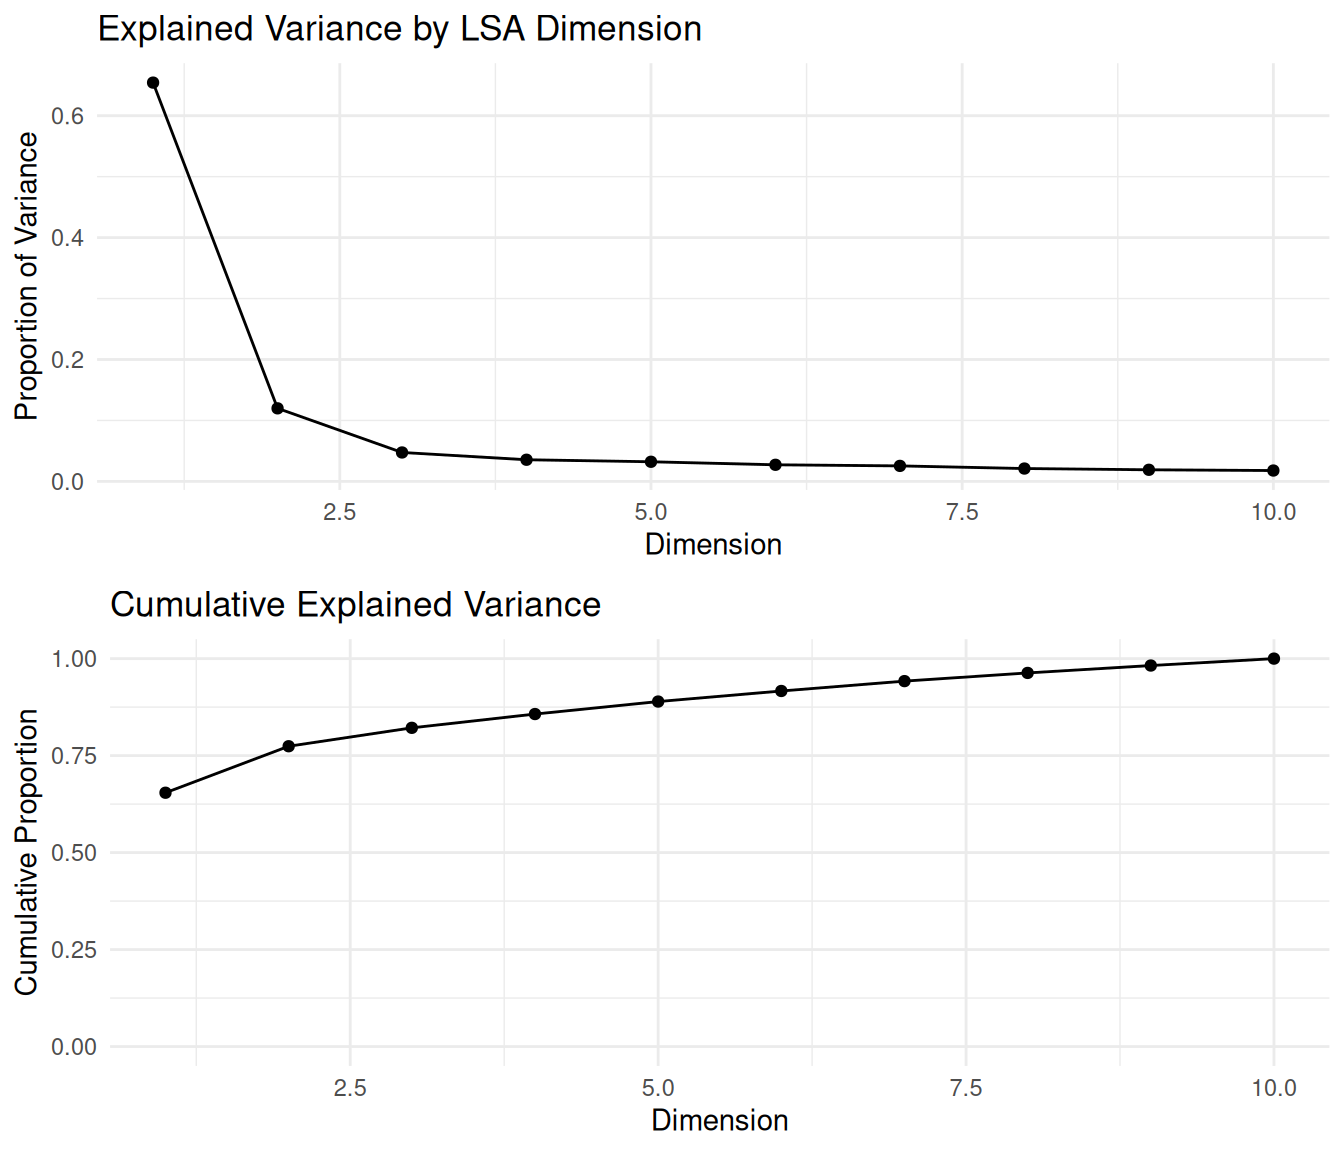
\includegraphics[keepaspectratio]{Introduction-to-Quantitative-Text-Analysis_files/figure-latex/lsa-explained-variance-plots-1.pdf}}

These plots help us determine the ideal number of dimensions to retain by identifying where the cumulative curve levels off---a common strategy known as the ``elbow method.'' Choosing the dimensionality is a trade-off between reducing noise and computational complexity versus preserving semantic information.

Another way to validate LSA is to examine whether semantically similar words are close together in the latent space. We compute the cosine similarity between LSA-generated vectors for selected terms. Terms used in similar contexts should have high cosine similarity in the LSA space.

\begin{Shaded}
\begin{Highlighting}[]
\FunctionTok{library}\NormalTok{(coop)  }\CommentTok{\# Need to install: install.packages(\textquotesingle{}coop\textquotesingle{})}
\end{Highlighting}
\end{Shaded}

\begin{verbatim}
## 
## Caricamento pacchetto: 'coop'
\end{verbatim}

\begin{verbatim}
## Il seguente oggetto è mascherato da 'package:quanteda':
## 
##     sparsity
\end{verbatim}

\begin{Shaded}
\begin{Highlighting}[]
\NormalTok{term\_vectors }\OtherTok{\textless{}{-}}\NormalTok{ lsa\_model}\SpecialCharTok{$}\NormalTok{features}

\CommentTok{\# Choose a set of semantically related terms for validation.}
\NormalTok{selected\_terms }\OtherTok{\textless{}{-}} \FunctionTok{c}\NormalTok{(}\StringTok{"america"}\NormalTok{, }\StringTok{"united"}\NormalTok{, }\StringTok{"states"}\NormalTok{, }\StringTok{"freedom"}\NormalTok{, }\StringTok{"liberty"}\NormalTok{, }\StringTok{"war"}\NormalTok{, }\StringTok{"peace"}\NormalTok{)}

\NormalTok{selected\_term\_vectors }\OtherTok{\textless{}{-}}\NormalTok{ term\_vectors[selected\_terms, , drop }\OtherTok{=} \ConstantTok{FALSE}\NormalTok{]}
\NormalTok{term\_similarity }\OtherTok{\textless{}{-}} \FunctionTok{cosine}\NormalTok{(}\FunctionTok{t}\NormalTok{(selected\_term\_vectors))}
\end{Highlighting}
\end{Shaded}

We expect related terms (e.g., ``freedom'' and ``liberty'') to have high cosine similarity. This indicates that LSA captures semantic relationships effectively. Unrelated terms should have lower cosine similarity.

Similarly, we can validate whether semantically similar documents are close in the latent space. Again, we use cosine similarity on the LSA vectors of selected presidential speeches. Documents that discuss identical themes or are from similar historical periods might be expected to have a higher similarity.

\begin{Shaded}
\begin{Highlighting}[]
\NormalTok{doc\_vectors }\OtherTok{\textless{}{-}}\NormalTok{ lsa\_model}\SpecialCharTok{$}\NormalTok{docs}
\NormalTok{docnames\_all }\OtherTok{\textless{}{-}} \FunctionTok{docnames}\NormalTok{(inaugural\_dfm)  }\CommentTok{\# Get all document names.}

\CommentTok{\# Select documents of interest by their names for validation.}
\NormalTok{selected\_docs }\OtherTok{\textless{}{-}} \FunctionTok{c}\NormalTok{(}\StringTok{"1789{-}Washington"}\NormalTok{, }\StringTok{"1861{-}Lincoln"}\NormalTok{, }\StringTok{"2001{-}G.W.Bush"}\NormalTok{, }\StringTok{"2009{-}Obama"}\NormalTok{)}
\NormalTok{selected\_doc\_vectors }\OtherTok{\textless{}{-}}\NormalTok{ doc\_vectors[docnames\_all }\SpecialCharTok{\%in\%}\NormalTok{ selected\_docs, , drop }\OtherTok{=} \ConstantTok{FALSE}\NormalTok{]}

\CommentTok{\# Compute cosine similarity between selected document vectors.}
\NormalTok{doc\_similarity }\OtherTok{\textless{}{-}} \FunctionTok{cosine}\NormalTok{(}\FunctionTok{t}\NormalTok{(selected\_doc\_vectors))}
\end{Highlighting}
\end{Shaded}

By interpreting this matrix, we can observe whether documents from similar eras or with similar themes cluster together---an indicator that LSA is capturing meaningful structures. For instance, one might expect speeches from presidents in closer periods or from the same political party to exhibit higher similarity than those from vastly different eras or parties.

\section{Exercises}\label{exercises-4}

\begin{enumerate}
\def\labelenumi{\arabic{enumi}.}
\item
  Apply standard LDA to a different corpus (e.g.~UK party manifestos or movie reviews). Experiment with varying numbers of topics (k) and evaluate the topics qualitatively based on the most frequent words and quantitatively using semantic coherence and perplexity if these are available in the package used. Select an appropriate k and interpret the main topics found.
\item
  For the LDA model fitted in Exercise 1, visualise the document-topic distributions for a few selected documents. Which documents have the highest proportions of the most interesting topics? Validate your interpretation by examining the content of these documents. As part of your validation process, calculate and compare the log-likelihood or perplexity for models with different numbers of topics.
\item
  Create a custom dictionary with seed words relevant to a research question, then apply seeded LDA to a suitable corpus. Interpret the seeded topics and examine the dominant topic assignments per document. If available, compare the resulting top terms and document assignments to those from a standard LDA model on the same corpus as a form of validation.
\item
  Apply STM to a corpus with rich metadata (e.g.~a dataset of news articles containing the date and source or a corpus of speeches containing speaker attributes). Select a set of topics using searchK, carefully evaluating the diagnostic plots. Fit the STM model to the prevalence formula, including relevant metadata. Use estimateEffect() to analyse how the metadata affects the prevalence of specific topics, visualising the results and interpreting the significance of the effects as part of the validation process. Examine the `labelTopics()' output for qualitative validation of the topics.
\item
  Apply LSA to a corpus using the textmodel\_lsa function. Experiment with different numbers of dimensions (nd). Examine the term and document loadings for a selected number of dimensions, then try to interpret the latent concepts discovered by LSA. Calculate and visualise the cumulative explained variance by the dimensions to help select nd.
\item
  For your LSA model from Exercise 5, calculate and examine the cosine similarity between a few pairs of selected documents or terms that you expect to be similar or dissimilar based on your knowledge of the corpus. Assess whether the LSA similarity scores align with your expectations to validate the results.
\item
  Research and implement a method to compute topic coherence (e.g.~pointwise mutual information between top words) for an LDA or STM model, in cases where either \texttt{searchK} or \texttt{labelTopics} do not provide sufficient detail, or where another package is being used. Use this to quantitatively validate your chosen topic models and compare models with different k.
\end{enumerate}

\phantomsection\label{refs}
\begin{CSLReferences}{1}{2}
\bibitem[\citeproctext]{ref-Albaugh2013a}
Albaugh, Q., Sevenans, J., Soroka, S., \& Loewen, P. J. (2013). {The Automated Coding of Policy Agendas: A Dictionary-based Approach}. \emph{6th Annual Comparative Agendas Conference, Antwerp, Belgium}.

\bibitem[\citeproctext]{ref-Bakker2012a}
Bakker, R., Vries, C. de, Edwards, E., Hooghe, L., Jolly, S., Marks, G., Polk, J., Rovny, J., Steenbergen, M. R., \& Vachudova, M. A. (2012). Measuring party positions in europe: The chapel hill expert survey trend file, 1999-2010. \emph{Party Politics}, \emph{21}(1), 1--15. \url{https://doi.org/10.1177/1354068812462931}

\bibitem[\citeproctext]{ref-Benoit2009a}
Benoit, K., Laver, M., \& Mikhaylov, S. (2009). Treating words as data with error: Uncertainty in text statements of policy positions. \emph{American Journal of Political Science}, \emph{53}(2), 495--513. \url{https://doi.org/10.1111/j.1540-5907.2009.00383.x}

\bibitem[\citeproctext]{ref-Benoit2018a}
Benoit, K., Watanabe, K., Wang, H., Nulty, P., Obeng, A., Müller, S., \& Matsuo, A. (2018). Quanteda: An r package for the quantitative analysis of textual data. \emph{Journal of Open Source Software}, \emph{3}(30), 774. \url{https://doi.org/10.21105/joss.00774}

\bibitem[\citeproctext]{ref-Bruinsma2019a}
Bruinsma, B., \& Gemenis, K. (2019). {Validating Wordscores: The Promises and Pitfalls of Computational Text Scaling}. \emph{Communication Methods and Measures}, \emph{13}(3), 212--227. \url{https://doi.org/10.1080/19312458.2019.1594741}

\bibitem[\citeproctext]{ref-Carmines1979a}
Carmines, E. G., \& Zeller, R. A. (1979). \emph{Reliability and validity assessment}. Sage. \url{https://doi.org/10.4135/9781412985642}

\bibitem[\citeproctext]{ref-Clarke2019a}
Clarke, I., \& Grieve, J. (2019). Stylistic variation on the donald trump twitter account: A linguistic analysis of tweets posted between 2009 and 2018. \emph{PLOS ONE}, \emph{14}(9), 1--27. \url{https://doi.org/10.1371/journal.pone.0222062}

\bibitem[\citeproctext]{ref-Denny2018a}
Denny, M. J., \& Spirling, A. (2018). Text preprocessing for unsupervised learning: Why it matters, when it misleads, and what to do about it. \emph{Political Analysis}, \emph{26}(2), 168--189. \url{https://doi.org/10.1017/pan.2017.44}

\bibitem[\citeproctext]{ref-Grimmer2022a}
Grimmer, J., Roberts, M. E., \& Stewart, B. M. (2022). \emph{{Text as Data: A New Framework for Machine Learning and the Social Sciences}}. Princeton University Press.

\bibitem[\citeproctext]{ref-Grimmer2013a}
Grimmer, J., \& Stewart, B. M. (2013). Text as data: The promise and pitfals of automatic content analysis methods for political texts. \emph{Political Analysis}, \emph{21}(3), 267--297. \url{https://doi.org/10.1093/pan/mps028}

\bibitem[\citeproctext]{ref-Haselmayer2017a}
Haselmayer, M., \& Jenny, M. (2017). Sentiment analysis of political communication: Combining a dictionary approach with crowdcoding. \emph{Quality \& Quantity}, \emph{51}(6), 2623--2646. \url{https://doi.org/10.1007/s11135-016-0412-4}

\bibitem[\citeproctext]{ref-Hutto2014a}
Hutto, C., \& Gilbert, E. (2014). VADER: A parsimonious rule-based model for sentiment analysis of social media text. \emph{Proceedings of the International AAAI Conference on Web and Social Media}, \emph{8}(1), 216--225. \url{https://doi.org/10.1609/icwsm.v8i1.14550}

\bibitem[\citeproctext]{ref-Krippendorff2019a}
Krippendorff, K. (2019). \emph{{Content Analysis - An Introduction to Its Methodology}} (4th ed.). Sage. \url{https://doi.org/10.4135/9781071878781}

\bibitem[\citeproctext]{ref-Laver2003a}
Laver, M., Benoit, K., \& Garry, J. (2003). Extracting policy positions from political texts using words as data. \emph{The American Political Science Review}, \emph{97}(2), 311--331. \url{https://doi.org/10.1017/S0003055403000698}

\bibitem[\citeproctext]{ref-Laver2000a}
Laver, M., \& Garry, J. (2000). Estimating policy positions from political texts. \emph{American Journal of Political Science}, \emph{44}(3), 619--634. \url{https://doi.org/10.2307/2669268}

\bibitem[\citeproctext]{ref-Le2008a}
Lê, S., Josse, J., \& Husson, F. (2008). Factominer: An r package for multivariate analysis. \emph{Journal of Statistical Software}, \emph{25}(1). \url{https://doi.org/10.18637/jss.v025.i01}

\bibitem[\citeproctext]{ref-Lin1989a}
Lin, L. (1989). A concordance correlation coefficient to evaluate reproducibility. \emph{Biometrics}, \emph{45}, 255--268. \url{https://doi.org/10.2307/2532051}

\bibitem[\citeproctext]{ref-Lind2019a}
Lind, F., Eberl, J.-M., Heidenreich, T., \& Boomgaarden, H. G. (2019). When the journey is as important as the goal: A roadmap to multilingual dictionary construction. \emph{International Journal of Communication}, \emph{13}, 4000--4020.

\bibitem[\citeproctext]{ref-Lowe2011a}
Lowe, W., \& Benoit, K. (2011). Estimating uncertainty in quantitative text analysis. \emph{Annual Meeting of the Midwest Political Science Association}.

\bibitem[\citeproctext]{ref-Martin2008a}
Martin, L. W., \& Vanberg, G. (2008). Reply to benoit and laver. \emph{Political Analysis}, \emph{16}(1), 112--114. \url{https://doi.org/10.1093/pan/mpm018}

\bibitem[\citeproctext]{ref-Mikhaylov2012a}
Mikhaylov, S., Laver, M., \& Benoit, K. (2012). Coder reliability and misclassification in the human coding of party manifestos. \emph{Political Analysis}, \emph{20}(1), 78--91. \url{https://doi.org/10.1093/pan/mpr047}

\bibitem[\citeproctext]{ref-Neuendorf2017a}
Neuendorf, K. A. (2016). \emph{{The Content Analysis Guidebook}} (2nd ed.). Sage. \url{https://doi.org/10.4135/9781071802878}

\bibitem[\citeproctext]{ref-Slapin2008a}
Slapin, J. B., \& Proksch, S.-O. (2008). A scaling model for estimating time-series party positions from texts. \emph{American Journal of Political Science}, \emph{52}(3), 705--722. \url{https://doi.org/10.1111/j.1540-5907.2008.00338.x}

\bibitem[\citeproctext]{ref-Wickham2023a}
Wickham, H., Çetinkaya-Rundel, M., \& Grolemund, G. (2023). \emph{{R for Data Science}} (2nd ed.). \url{https://r4ds.hadley.nz/}

\bibitem[\citeproctext]{ref-Young2012a}
Young, L., \& Soroka, S. (2012). \emph{Lexicoder sentiment dictionary}. \url{http://www.snsoroka.com/data-lexicoder/}

\end{CSLReferences}

\end{document}
